% Options for packages loaded elsewhere
% Options for packages loaded elsewhere
\PassOptionsToPackage{unicode}{hyperref}
\PassOptionsToPackage{hyphens}{url}
\PassOptionsToPackage{dvipsnames,svgnames,x11names}{xcolor}
%
\documentclass[
  french,
  a4paper,
  DIV=11,
  numbers=noendperiod,
  oneside]{scrreprt}
\usepackage{xcolor}
\usepackage[left=1in,marginparwidth=2.0in,textwidth=4.0in,marginparsep=0.3in]{geometry}
\usepackage{amsmath,amssymb}
\setcounter{secnumdepth}{5}
\usepackage{iftex}
\ifPDFTeX
  \usepackage[T1]{fontenc}
  \usepackage[utf8]{inputenc}
  \usepackage{textcomp} % provide euro and other symbols
\else % if luatex or xetex
  \usepackage{unicode-math} % this also loads fontspec
  \defaultfontfeatures{Scale=MatchLowercase}
  \defaultfontfeatures[\rmfamily]{Ligatures=TeX,Scale=1}
\fi
\usepackage{lmodern}
\ifPDFTeX\else
  % xetex/luatex font selection
\fi
% Use upquote if available, for straight quotes in verbatim environments
\IfFileExists{upquote.sty}{\usepackage{upquote}}{}
\IfFileExists{microtype.sty}{% use microtype if available
  \usepackage[]{microtype}
  \UseMicrotypeSet[protrusion]{basicmath} % disable protrusion for tt fonts
}{}
\makeatletter
\@ifundefined{KOMAClassName}{% if non-KOMA class
  \IfFileExists{parskip.sty}{%
    \usepackage{parskip}
  }{% else
    \setlength{\parindent}{0pt}
    \setlength{\parskip}{6pt plus 2pt minus 1pt}}
}{% if KOMA class
  \KOMAoptions{parskip=half}}
\makeatother
% Make \paragraph and \subparagraph free-standing
\makeatletter
\ifx\paragraph\undefined\else
  \let\oldparagraph\paragraph
  \renewcommand{\paragraph}{
    \@ifstar
      \xxxParagraphStar
      \xxxParagraphNoStar
  }
  \newcommand{\xxxParagraphStar}[1]{\oldparagraph*{#1}\mbox{}}
  \newcommand{\xxxParagraphNoStar}[1]{\oldparagraph{#1}\mbox{}}
\fi
\ifx\subparagraph\undefined\else
  \let\oldsubparagraph\subparagraph
  \renewcommand{\subparagraph}{
    \@ifstar
      \xxxSubParagraphStar
      \xxxSubParagraphNoStar
  }
  \newcommand{\xxxSubParagraphStar}[1]{\oldsubparagraph*{#1}\mbox{}}
  \newcommand{\xxxSubParagraphNoStar}[1]{\oldsubparagraph{#1}\mbox{}}
\fi
\makeatother

\usepackage{color}
\usepackage{fancyvrb}
\newcommand{\VerbBar}{|}
\newcommand{\VERB}{\Verb[commandchars=\\\{\}]}
\DefineVerbatimEnvironment{Highlighting}{Verbatim}{commandchars=\\\{\}}
% Add ',fontsize=\small' for more characters per line
\newenvironment{Shaded}{}{}
\newcommand{\AlertTok}[1]{\textcolor[rgb]{1.00,0.33,0.33}{\textbf{#1}}}
\newcommand{\AnnotationTok}[1]{\textcolor[rgb]{0.42,0.45,0.49}{#1}}
\newcommand{\AttributeTok}[1]{\textcolor[rgb]{0.84,0.23,0.29}{#1}}
\newcommand{\BaseNTok}[1]{\textcolor[rgb]{0.00,0.36,0.77}{#1}}
\newcommand{\BuiltInTok}[1]{\textcolor[rgb]{0.84,0.23,0.29}{#1}}
\newcommand{\CharTok}[1]{\textcolor[rgb]{0.01,0.18,0.38}{#1}}
\newcommand{\CommentTok}[1]{\textcolor[rgb]{0.42,0.45,0.49}{#1}}
\newcommand{\CommentVarTok}[1]{\textcolor[rgb]{0.42,0.45,0.49}{#1}}
\newcommand{\ConstantTok}[1]{\textcolor[rgb]{0.00,0.36,0.77}{#1}}
\newcommand{\ControlFlowTok}[1]{\textcolor[rgb]{0.84,0.23,0.29}{#1}}
\newcommand{\DataTypeTok}[1]{\textcolor[rgb]{0.84,0.23,0.29}{#1}}
\newcommand{\DecValTok}[1]{\textcolor[rgb]{0.00,0.36,0.77}{#1}}
\newcommand{\DocumentationTok}[1]{\textcolor[rgb]{0.42,0.45,0.49}{#1}}
\newcommand{\ErrorTok}[1]{\textcolor[rgb]{1.00,0.33,0.33}{\underline{#1}}}
\newcommand{\ExtensionTok}[1]{\textcolor[rgb]{0.84,0.23,0.29}{\textbf{#1}}}
\newcommand{\FloatTok}[1]{\textcolor[rgb]{0.00,0.36,0.77}{#1}}
\newcommand{\FunctionTok}[1]{\textcolor[rgb]{0.44,0.26,0.76}{#1}}
\newcommand{\ImportTok}[1]{\textcolor[rgb]{0.01,0.18,0.38}{#1}}
\newcommand{\InformationTok}[1]{\textcolor[rgb]{0.42,0.45,0.49}{#1}}
\newcommand{\KeywordTok}[1]{\textcolor[rgb]{0.84,0.23,0.29}{#1}}
\newcommand{\NormalTok}[1]{\textcolor[rgb]{0.14,0.16,0.18}{#1}}
\newcommand{\OperatorTok}[1]{\textcolor[rgb]{0.14,0.16,0.18}{#1}}
\newcommand{\OtherTok}[1]{\textcolor[rgb]{0.44,0.26,0.76}{#1}}
\newcommand{\PreprocessorTok}[1]{\textcolor[rgb]{0.84,0.23,0.29}{#1}}
\newcommand{\RegionMarkerTok}[1]{\textcolor[rgb]{0.42,0.45,0.49}{#1}}
\newcommand{\SpecialCharTok}[1]{\textcolor[rgb]{0.00,0.36,0.77}{#1}}
\newcommand{\SpecialStringTok}[1]{\textcolor[rgb]{0.01,0.18,0.38}{#1}}
\newcommand{\StringTok}[1]{\textcolor[rgb]{0.01,0.18,0.38}{#1}}
\newcommand{\VariableTok}[1]{\textcolor[rgb]{0.89,0.38,0.04}{#1}}
\newcommand{\VerbatimStringTok}[1]{\textcolor[rgb]{0.01,0.18,0.38}{#1}}
\newcommand{\WarningTok}[1]{\textcolor[rgb]{1.00,0.33,0.33}{#1}}

\usepackage{longtable,booktabs,array}
\newcounter{none} % for unnumbered tables
\usepackage{calc} % for calculating minipage widths
% Correct order of tables after \paragraph or \subparagraph
\usepackage{etoolbox}
\makeatletter
\patchcmd\longtable{\par}{\if@noskipsec\mbox{}\fi\par}{}{}
\makeatother
% Allow footnotes in longtable head/foot
\IfFileExists{footnotehyper.sty}{\usepackage{footnotehyper}}{\usepackage{footnote}}
\makesavenoteenv{longtable}
\usepackage{graphicx}
\makeatletter
\newsavebox\pandoc@box
\newcommand*\pandocbounded[1]{% scales image to fit in text height/width
  \sbox\pandoc@box{#1}%
  \Gscale@div\@tempa{\textheight}{\dimexpr\ht\pandoc@box+\dp\pandoc@box\relax}%
  \Gscale@div\@tempb{\linewidth}{\wd\pandoc@box}%
  \ifdim\@tempb\p@<\@tempa\p@\let\@tempa\@tempb\fi% select the smaller of both
  \ifdim\@tempa\p@<\p@\scalebox{\@tempa}{\usebox\pandoc@box}%
  \else\usebox{\pandoc@box}%
  \fi%
}
% Set default figure placement to htbp
\def\fps@figure{htbp}
\makeatother


% definitions for citeproc citations
\NewDocumentCommand\citeproctext{}{}
\NewDocumentCommand\citeproc{mm}{%
  \begingroup\def\citeproctext{#2}\cite{#1}\endgroup}
\makeatletter
 % allow citations to break across lines
 \let\@cite@ofmt\@firstofone
 % avoid brackets around text for \cite:
 \def\@biblabel#1{}
 \def\@cite#1#2{{#1\if@tempswa , #2\fi}}
\makeatother
\newlength{\cslhangindent}
\setlength{\cslhangindent}{1.5em}
\newlength{\csllabelwidth}
\setlength{\csllabelwidth}{3em}
\newenvironment{CSLReferences}[2] % #1 hanging-indent, #2 entry-spacing
 {\begin{list}{}{%
  \setlength{\itemindent}{0pt}
  \setlength{\leftmargin}{0pt}
  \setlength{\parsep}{0pt}
  % turn on hanging indent if param 1 is 1
  \ifodd #1
   \setlength{\leftmargin}{\cslhangindent}
   \setlength{\itemindent}{-1\cslhangindent}
  \fi
  % set entry spacing
  \setlength{\itemsep}{#2\baselineskip}}}
 {\end{list}}
\usepackage{calc}
\newcommand{\CSLBlock}[1]{\hfill\break\parbox[t]{\linewidth}{\strut\ignorespaces#1\strut}}
\newcommand{\CSLLeftMargin}[1]{\parbox[t]{\csllabelwidth}{\strut#1\strut}}
\newcommand{\CSLRightInline}[1]{\parbox[t]{\linewidth - \csllabelwidth}{\strut#1\strut}}
\newcommand{\CSLIndent}[1]{\hspace{\cslhangindent}#1}

\ifLuaTeX
\usepackage[bidi=basic,shorthands=off]{babel}
\else
\usepackage[bidi=default,shorthands=off]{babel}
\fi
\ifLuaTeX
  \usepackage{selnolig} % disable illegal ligatures
\fi


\setlength{\emergencystretch}{3em} % prevent overfull lines

\providecommand{\tightlist}{%
  \setlength{\itemsep}{0pt}\setlength{\parskip}{0pt}}



 


\usepackage{booktabs}
\usepackage{longtable}
\usepackage{array}
\usepackage{multirow}
\usepackage{wrapfig}
\usepackage{float}
\usepackage{colortbl}
\usepackage{pdflscape}
\usepackage{tabularx}
\usepackage{xltabular}
\usepackage{threeparttable}
\usepackage{threeparttablex}
\usepackage[normalem]{ulem}
\usepackage{makecell}
\usepackage{xcolor}
\KOMAoption{captions}{tableheading}
\makeatletter
\@ifpackageloaded{tcolorbox}{}{\usepackage[skins,breakable]{tcolorbox}}
\@ifpackageloaded{fontawesome5}{}{\usepackage{fontawesome5}}
\definecolor{quarto-callout-color}{HTML}{909090}
\definecolor{quarto-callout-note-color}{HTML}{0758E5}
\definecolor{quarto-callout-important-color}{HTML}{CC1914}
\definecolor{quarto-callout-warning-color}{HTML}{EB9113}
\definecolor{quarto-callout-tip-color}{HTML}{00A047}
\definecolor{quarto-callout-caution-color}{HTML}{FC5300}
\definecolor{quarto-callout-color-frame}{HTML}{acacac}
\definecolor{quarto-callout-note-color-frame}{HTML}{4582ec}
\definecolor{quarto-callout-important-color-frame}{HTML}{d9534f}
\definecolor{quarto-callout-warning-color-frame}{HTML}{f0ad4e}
\definecolor{quarto-callout-tip-color-frame}{HTML}{02b875}
\definecolor{quarto-callout-caution-color-frame}{HTML}{fd7e14}
\makeatother
\makeatletter
\@ifpackageloaded{bookmark}{}{\usepackage{bookmark}}
\makeatother
\makeatletter
\@ifpackageloaded{caption}{}{\usepackage{caption}}
\AtBeginDocument{%
\ifdefined\contentsname
  \renewcommand*\contentsname{Table des matières}
\else
  \newcommand\contentsname{Table des matières}
\fi
\ifdefined\listfigurename
  \renewcommand*\listfigurename{Liste des Figures}
\else
  \newcommand\listfigurename{Liste des Figures}
\fi
\ifdefined\listtablename
  \renewcommand*\listtablename{Liste des Tables}
\else
  \newcommand\listtablename{Liste des Tables}
\fi
\ifdefined\figurename
  \renewcommand*\figurename{Figure}
\else
  \newcommand\figurename{Figure}
\fi
\ifdefined\tablename
  \renewcommand*\tablename{Table}
\else
  \newcommand\tablename{Table}
\fi
}
\@ifpackageloaded{float}{}{\usepackage{float}}
\floatstyle{ruled}
\@ifundefined{c@chapter}{\newfloat{codelisting}{h}{lop}}{\newfloat{codelisting}{h}{lop}[chapter]}
\floatname{codelisting}{Listing}
\newcommand*\listoflistings{\listof{codelisting}{Liste des Listings}}
\makeatother
\makeatletter
\makeatother
\makeatletter
\@ifpackageloaded{caption}{}{\usepackage{caption}}
\@ifpackageloaded{subcaption}{}{\usepackage{subcaption}}
\makeatother
\makeatletter
\@ifpackageloaded{tcolorbox}{}{\usepackage[skins,breakable]{tcolorbox}}
\makeatother
\makeatletter
\@ifundefined{shadecolor}{\definecolor{shadecolor}{HTML}{31BAE9}}{}
\makeatother
\makeatletter
\makeatother
\makeatletter
\ifdefined\Shaded\renewenvironment{Shaded}{\begin{tcolorbox}[borderline west={3pt}{0pt}{shadecolor}, boxrule=0pt, breakable, enhanced, frame hidden, interior hidden, sharp corners]}{\end{tcolorbox}}\fi
\makeatother
\makeatletter
\@ifpackageloaded{sidenotes}{}{\usepackage{sidenotes}}
\@ifpackageloaded{marginnote}{}{\usepackage{marginnote}}
\makeatother
\makeatletter
\@ifpackageloaded{fontawesome5}{}{\usepackage{fontawesome5}}
\makeatother
\usepackage{bookmark}
\IfFileExists{xurl.sty}{\usepackage{xurl}}{} % add URL line breaks if available
\urlstyle{same}
% fallback for those not using the hyperref driver hyperxmp:
\makeatletter
\@ifundefined{xmpquote}{\newcommand{\xmpquote}[1]{#1}}{}
\makeatother
\hypersetup{
  pdftitle={TP de Biométrie  Semestre 5 },
  pdfauthor={Benoît Simon-Bouhet},
  pdflang={fr},
  colorlinks=true,
  linkcolor={blue},
  filecolor={Maroon},
  citecolor={Blue},
  urlcolor={Blue},
  pdfcreator={LaTeX via pandoc}}


\title{TP de Biométrie Semestre 5}
\author{Benoît Simon-Bouhet}
\date{vendredi 4 septembre 2026}
\begin{document}
\maketitle

\renewcommand*\contentsname{Table des matières}
{
\setcounter{tocdepth}{2}
\tableofcontents
}

\bookmarksetup{startatroot}

\chapter*{Introduction}\label{introduction}
\addcontentsline{toc}{chapter}{Introduction}

\markboth{Introduction}{Introduction}

\section*{Objectifs}\label{objectifs}
\addcontentsline{toc}{section}{Objectifs}

\markright{Objectifs}

Ce livre contient l'ensemble du matériel (contenus, exemples,
exercices\ldots) nécessaire à la réalisation des travaux pratiques de
\textbf{Biométrie} de l'EC \emph{Outils pour l'étude et la compréhension
du vivant 4} du semestre 5 de la licence Sciences de la Vie de La
Rochelle Université.

À la fin du semestre, vous devriez être capables de faire les choses
suivantes dans \texttt{RStudio} :

\begin{itemize}
\tightlist
\item
  Mettre en forme des tableaux de données : renommer des variables, en
  créer de nouvelles, modifier des variables existantes, filtrer des
  lignes, sélectionner des colonnes, etc. (vu au semestre 3)
\item
  Explorer des jeux de données en produisant des graphiques appropriés
  selon la nature des variables disponibles, leur nombre et l'objectif
  recherché (vu au semestre 3)
\item
  Explorer des jeux de données en produisant des résumés statistiques de
  variables de différentes nature (numériques continues ou
  catégorielles) et pour différentes modalités de facteurs d'intérêt (vu
  au semestre 4)
\item
  Calculer des indices de position (moyennes, médianes\ldots), de
  dispersion (écart-types, variances, IQR\ldots) et d'incertitude
  (erreurs standard, intervalles de confiance\ldots) pour plusieurs
  sous-groupes de vos jeux de données, et les représenter sur des
  graphiques adaptés (vu au semestre 4)
\item
  Choisir et formuler des hypothèses adaptées à la question scientifique
  posée (hypothèses bilatérales ou unilatérales)
\item
  Choisir les tests statistiques permettant de répondre à une question
  scientifique précise selon la nature de la question posée et la nature
  des variables à disposition
\item
  Réaliser les tests usuels de comparaison de moyennes (\(t\) de Student
  à 1 ou 2 échantillons, appariés ou indépendants\ldots)
\item
  Vérifier les conditions d'application des tests (graphiquement et avec
  des tests appropriés tels que les test de Shapiro-Wilk et de Levene),
  et le cas échéant, réaliser des tests non paramétriques équivalents
  (test de Welch, de Wilcoxon\ldots)
\item
  Interpréter correctement les résultats des tests pour répondre aux
  questions scientifiques posées
\item
  Identifier des cohortes dans une population et en étudier les
  caractéristiques et l'évolution temporelle
\item
  Simuler le comportement de populations théoriques simples suivant des
  modèles démographiques précis (mortalité exponentielle, croissance
  exponentielle, croissance logistique, système prédateur-proies de
  Lotka et Volterra, et systèmes de compétition à 2 ou 3 espèces\ldots)
\item
  Simuler, par chaînes de Markov, les successions écologiques dans un
  écosystème théorique
\end{itemize}

\section*{Pré-requis}\label{pruxe9-requis}
\addcontentsline{toc}{section}{Pré-requis}

\markright{Pré-requis}

Pour atteindre les objectifs fixés ici, et compte tenu du volume horaire
restreint qui est consacré aux TP et TEA de Biométrie au S5, je suppose
que vous possédez un certain nombre de pré-requis. En particulier, vous
devriez avoir à ce stade une bonne connaissance de l'interface du
logiciel \texttt{RStudio}, et vous devriez être capables :

\begin{enumerate}
\def\labelenumi{\arabic{enumi}.}
\tightlist
\item
  de créer un \texttt{Rproject} et un script d'analyse dans
  \texttt{RStudio}
\item
  d'importer des jeux de données issus de tableurs dans \texttt{RStudio}
\item
  d'effectuer des manipulations de données simples (sélectionner des
  variables, trier des colonnes, filtrer des lignes, créer de nouvelles
  variables, etc.)
\item
  de produire des graphiques de qualité, adaptés à la fois aux variables
  dont vous disposez et aux questions auxquelles vous souhaitez répondre
\item
  de réaliser une exploration statistique de vos données en calculant
  des indices de position, de dispersion et d'incertitude pour plusieurs
  sous-groupes de vos données
\end{enumerate}

\begin{tcolorbox}[enhanced jigsaw, arc=.35mm, bottomrule=.15mm, bottomtitle=1mm, breakable, colback=white, colbacktitle=quarto-callout-warning-color!10!white, colframe=quarto-callout-warning-color-frame, coltitle=black, left=2mm, leftrule=.75mm, opacityback=0, opacitybacktitle=0.6, rightrule=.15mm, title=\textcolor{quarto-callout-warning-color}{\faExclamationTriangle}\hspace{0.5em}{Si ces pré-requis ne sont pas maîtrisés}, titlerule=0mm, toprule=.15mm, toptitle=1mm]

Mettez-vous à niveau de toute urgence en lisant attentivement :

\begin{itemize}
\tightlist
\item
  \href{https://besibo.github.io/BiometrieS3/}{le livre en ligne de
  Biométrie du semestre 3}
\item
  \href{https://besibo.github.io/BiometrieS4/}{le livre en ligne de
  Biométrie du semestre 4}
\end{itemize}

Vous aurez de toutes façons besoin de vous référer à ces 2 documents
régulièrement au cours de ces TP. Donc gardez-les à portée de main et
apprenez à naviguez rapidement dans leurs chapitres et sous-chapitres
pour retrouver facilement les informations dont vous avez besoin.

\end{tcolorbox}

\section*{Organisation}\label{organisation}
\addcontentsline{toc}{section}{Organisation}

\markright{Organisation}

\subsection*{Volume de travail}\label{volume-de-travail}
\addcontentsline{toc}{subsection}{Volume de travail}

Les travaux pratiques et TEA de biométrie auront lieu entre le 29
septembre et le 21 novembre 2025. Durant cette période, un créneau
d'1h30 de TP (pour chaque groupe) et un créneau d'1h30 de TEA (pour la
promotion entière) sont prévus chaque semaine, sauf pendant les vacances
de la Toussaint. Attention, certains TP sont prévus jusqu'à 18h15
heures, et les TEA ont souvent lieu le samedi matin.

\textbf{Les séances de TP ont lieu soit en salle MSI 217, soit dans les
salles du Pôle Communication Multimédia Réseau (PCMR). Tous les TEA sont
à distance.}

Au total, chaque groupe aura donc 7 séances de TP et 7 séances de TEA,
soit un total de 21 heures prévues dans vos emplois du temps. C'est peu
pour atteindre les objectifs fixés et il y aura donc évidemment du
travail personnel à fournir en dehors de ces séances. J'estime que vous
devrez fournir à peu près une vingtaine d'heures de travail personnel en
plus des séances prévues dans votre emploi du temps. Attention donc :
pensez bien à prévoir du temps dans vos plannings car le travail
personnel est essentiel pour progresser dans cette matière. J'insiste
sur l'importance de faire l'effort dès maintenant : vous allez en effet
avoir des enseignements qui reposent sur l'utilisation de ces logiciels
jusqu'à la fin du S6 (y compris pendant vos stage et, très
vraisemblablement, dans vos futurs masters également). C'est donc
maintenant qu'il faut acquérir des automatismes, cela vous fera gagner
énormément de temps ensuite. Prévoyez donc de consacrer environ 6h00 par
semaine à cette matière (3h prévues dans vos emplois du temps, et 3h de
travail personnel).

\subsection*{Modalités d'enseignement}\label{modalituxe9s-denseignement}
\addcontentsline{toc}{subsection}{Modalités d'enseignement}

Pour suivre cet enseignement vous pourrez utiliser les ordinateurs de
l'université, mais je ne peux que vous encourager à utiliser vos propres
ordinateurs, sous Windows, Linux ou MacOS. Lors de vos futurs stages et
pour rédiger vos comptes-rendus de TP, vous utiliserez le plus souvent
vos propres ordinateurs, autant prendre dès maintenant de bonnes
habitudes en installant les logiciels dont vous aurez besoin tout au
long de votre licence. Si vous n'avez pas suivi les cours de biométrie
de L2 et que les logiciels \texttt{R} et \texttt{RStudio} ne sont pas
encore installés sur vos ordinateurs, suivez
\href{https://besibo.github.io/BiometrieS3/01-R-basics.html\#sec-install}{la
procédure décrite ici}. Si vous ne possédez pas d'ordinateur, manifestez
vous rapidement auprès de moi car des solutions existent (prêt par
l'université, travail sur tablette ou chromebook via
\href{https://posit.cloud}{Posit cloud}\ldots).

\begin{tcolorbox}[enhanced jigsaw, arc=.35mm, bottomrule=.15mm, bottomtitle=1mm, breakable, colback=white, colbacktitle=quarto-callout-important-color!10!white, colframe=quarto-callout-important-color-frame, coltitle=black, left=2mm, leftrule=.75mm, opacityback=0, opacitybacktitle=0.6, rightrule=.15mm, title=\textcolor{quarto-callout-important-color}{\faExclamation}\hspace{0.5em}{Important}, titlerule=0mm, toprule=.15mm, toptitle=1mm]

L'essentiel du contenu de cet enseignement peut être abordé en
autonomie, à distance, grâce à ce livre en ligne, aux ressources mises à
disposition sur Moodle et à votre ordinateur personnel. Cela signifie
que \textbf{la présence physique lors desTP n'est pas obligatoire pour
toutes les séances}.

\end{tcolorbox}

Plus que des séances de TP classiques, considérez plutôt qu'il s'agit de
\textbf{permanences non-obligatoires} : si vous pensez avoir besoin
d'aide, si vous avez des points de blocage ou des questions sur le
contenu de ce document ou sur les exercices demandés, alors venez poser
vos questions lors des séances de TP. Vous ne serez d'ailleurs pas tenus
de rester pendant 1h30 : si vous obtenez une réponse en 10 minutes et
que vous préférez travailler ailleurs, vous serez libres de repartir !

De même, si vous n'avez pas de difficulté de compréhension, que vous
n'avez pas de problème avec les exercices de ce livre en ligne ni avec
les quizz Moodle, votre présence n'est pas requise. Si vous souhaitez
malgré tout venir en salle de TP, pas de problème, vous y serez toujours
les bienvenus.

Ce fonctionnement très souple a de nombreux avantages :

\begin{itemize}
\tightlist
\item
  vous vous organisez comme vous le souhaitez
\item
  vous ne venez que lorsque vous en avez vraiment besoin
\item
  celles et ceux qui se déplacent reçoivent une aide personnalisée
\item
  vous travaillez sur vos ordinateurs
\item
  les effectifs étant réduits, c'est aussi plus confortable pour moi !
\end{itemize}

Toutefois, pour que cette organisation fonctionne, cela demande de la
rigueur de votre part, en particulier sur la régularité du travail que
vous devez fournir. Si la présence en salle de TP n'est pas requise,
\textbf{le travail demandé est bel et bien obligatoire} ! Si vous venez
en salle de TP sans avoir travaillé en amont, votre venue sera
totalement inutile puisque vous n'aurez pas de question à poser et que
vous passerez votre séance à lire et suivre ce livre en ligne, choses
que vous pouvez très bien faire chez vous. Vous perdrez donc votre
temps, celui de vos collègues, et le mien. De même, si vous attendez la
4e semaine pour vous y mettre, vous irez droit dans le mur. Je le
répète, outre les heures de TP/TEA prévus dans vos emplois du temps,
vous devez prévoir au moins 20 heures de travail personnel
supplémentaire.

Je vous laisse donc une grande liberté d'organisation. À vous d'en tirer
le maximum et de faire preuve du sérieux nécessaire. Le rythme auquel
vous devriez avancer est présenté dans la partie suivante intitulée
``Progression conseillée''.

\begin{tcolorbox}[enhanced jigsaw, arc=.35mm, bottomrule=.15mm, bottomtitle=1mm, breakable, colback=white, colbacktitle=quarto-callout-important-color!10!white, colframe=quarto-callout-important-color-frame, coltitle=black, left=2mm, leftrule=.75mm, opacityback=0, opacitybacktitle=0.6, rightrule=.15mm, title=\textcolor{quarto-callout-important-color}{\faExclamation}\hspace{0.5em}{Important}, titlerule=0mm, toprule=.15mm, toptitle=1mm]

Attention !

Le mode ``permanance non obligatoire'' n'est valable que pour les 4
premières séances de TP, qui portent sur les tests de comparaison de
moyennes. Pour les 3 dernières séances, qui portent sur le cours de
fonctionnement des écosystèmes, qui seront assurées par Florian Orgeret,
et qui sont plus éloignées de ce que vous avez déjà vu dans vos
précédents enseignements de biométrie, votre présence en salle de TP
sera \textbf{obligatoire}, comme pour un TP classique.

\end{tcolorbox}

\subsection*{Utilisation de Slack}\label{utilisation-de-slack}
\addcontentsline{toc}{subsection}{Utilisation de Slack}

Outre les séances de permanence non-obligatoires, nous échangerons aussi
sur \href{https://slack.com/intl/fr-fr/}{l'application Slack}, qui
fonctionne un peu comme un ``twitter privé''. Slack facilite la
communication des équipes et permet de travailler ensemble. Créez-vous
un compte en ligne et installez le logiciel sur votre ordinateur (il
existe aussi des versions pour tablettes et smartphones). Lorsque vous
aurez installé le logiciel,
\href{https://join.slack.com/t/l3sv25-26/shared_invite/zt-3e5w5venb-ksvbjpQfhF9h~yBUFKBlBg}{cliquez
sur ce lien} pour vous connecter à notre espace de travail commun
intitulé \texttt{L3\ SV\ 25-26} (ce lien expire régulièrement : faites
moi signe s'il n'est plus valide).

Vous verrez que 3 ``chaînes'' sont disponibles :

\begin{itemize}
\tightlist
\item
  \#général : c'est là que les questions liées à l'organisation générale
  du cours, des TP et TEA, des évaluations, etc. doivent être posées. Si
  vous ne savez pas si une séance de permanence a lieu, posez la
  question ici.
\item
  \#questions-rstudio : c'est ici que toutes les questions pratiques
  liées à l'utilisation de \texttt{R} et \texttt{RStudio} devront êtres
  posées. Problèmes de syntaxe, problèmes liés à l'interface, à
  l'installation des packages ou à l'utilisation des fonctions, à la
  création des graphiques, à la manipulation des tableaux\ldots{} Tout
  ce qui concerne directement les logiciels sera traité ici. Vous êtes
  libres de poser des questions, de poster des captures d'écran, des
  morceaux de code, des messages d'erreur. Et \textbf{vous êtes bien
  entendus vivement encouragés à vous entraider et à répondre aux
  questions de vos collègues.} Je n'interviendrai ici que pour répondre
  aux questions laissées sans réponse ou si les réponses apportées sont
  inexactes. Le fonctionnement est celui d'un forum de discussion
  instantané. Vous en tirerez le plus grand bénéfice en participant et
  en n'ayant pas peur de poser des questions, même si elles vous
  paraissent idiotes. Rappelez-vous toujours que si vous vous posez une
  question, d'autres se la posent aussi probablement.
\item
  \#questions-stats : C'est ici que vous pourrez poser vos questions
  liées aux méthodes statistiques ou aux choix des modèles de dynamique
  des populations. Tout ce qui ne concerne pas directement l'utilisation
  du logiciel (comme par exemple le choix d'un test ou des hypothèses
  nulles et alternatives, la démarche d'analyse, la signification de tel
  paramètre ou estimateur, le principe de telle ou telle méthode\ldots)
  peut être discuté ici. Comme pour le canal \#questions-rstudio,
  \textbf{vous êtes encouragés à vous entraider et à répondre aux
  questions de vos collègues}.
\end{itemize}

Ainsi, quand vous travaillerez à vos TP ou TEA, que vous soyez installés
chez vous ou en salle de TP, prenez l'habitude de garder Slack ouvert
sur votre ordinateur. Même si vous n'avez pas de question à poser, votre
participation active pour répondre à vos collègues est souhaitable et
souhaitée. Je vous incite donc fortement à vous \textbf{entraider} :
c'est très formateur pour celui qui explique, et celui qui rencontre une
difficulté a plus de chances de comprendre si c'est quelqu'un d'autre
qui lui explique plutôt que la personne qui a rédigé les instructions
mal comprises.

Ce document est fait pour vous permettre d'avancer en autonomie et vous
ne devriez normalement pas avoir beaucoup besoin de moi si votre lecture
est attentive. L'expérience montre en effet que la plupart du temps, il
suffit de lire correctement les paragraphes précédents et/ou suivants
pour obtenir la réponse à ses questions. J'essaie néanmoins de rester
disponible sur Slack pendant les séances de TP et de TEA de tous les
groupes. Cela veut donc dire que \textbf{même si votre groupe n'est pas
en TP, vos questions ont des chances d'être lues et de recevoir des
réponses dès que d'autres groupes sont en TP ou TEA}. Vous êtes
d'ailleurs encouragés à échanger sur Slack aussi pendant vos phases de
travail personnel.

\section*{Progression conseillée}\label{progression-conseilluxe9e}
\addcontentsline{toc}{section}{Progression conseillée}

\markright{Progression conseillée}

Si vous avez suivi le document de prise en main de \texttt{R} et
\texttt{RStudio} lors de l'EC de biométrie du semestre 3 de la licence
SV de La Rochelle, vous savez que pour apprendre à utiliser ces
logiciels, il faut faire les choses soi-même, ne pas avoir peur des
messages d'erreurs (il faut d'ailleurs apprendre à les déchiffrer pour
comprendre d'où viennent les problèmes), essayer maintes fois, se
tromper beaucoup, recommencer, et surtout, ne pas se décourager.
J'utilise ce logiciel presque quotidiennement depuis plus de 15 ans et à
chaque session de travail, je rencontre des messages d'erreur. Avec
suffisamment d'habitude, on apprend à les déchiffrer et on corrige les
problèmes en quelques secondes. Ce livre est conçu pour vous faciliter
la tâche, mais ne vous y trompez pas, vous rencontrerez des difficultés,
et c'est normal. C'est le prix à payer pour profiter de la puissance du
meilleur logiciel permettant d'analyser des données, de produire des
graphiques de qualité et de réaliser toutes les statistiques dont vous
aurez besoin d'ici la fin de vos études et au-delà.

Pour que cet apprentissage soit le moins problématique possible, il
convient de prendre les choses dans l'ordre. C'est la raison pour
laquelle les chapitres de ce livre doivent être lus dans l'ordre, et les
exercices d'application faits au fur et à mesure de la lecture.

Idéalement, voilà les étapes que vous devriez avoir franchi chaque
semaine :

\begin{enumerate}
\def\labelenumi{\arabic{enumi}.}
\item
  Les deux premières séances sont consacrées à la comparaison de la
  moyenne d'une population à une valeur théorique
  (Chapitre~\ref{sec-moy1}). Si vous êtes déjà capable d'importer et
  manipuler des données dans \texttt{R}, ainsi que de les explorer
  graphiquement et par le calcul d'indices de statistiques descriptives
  (indices de position, de dispersion et d'incertitude), les fonctions
  nouvelles seront peu nombreuses. Mais ce chapitre est l'occasion
  d'aborder des notions complexes (test paramétrique ou non, hypothèses
  nulles et alternatives, \(p-\)value, décision, erreurs, puissance,
  etc.) qui demanderont une lecture très attentive. C'est également la
  première fois que vous serez confronté à toutes les étapes d'une
  analyse de données : de l'importation des données dans
  \texttt{RStudio} jusqu'à la réalisation des tests statistiques et leur
  interprétation, en passant par le calcul des statistiques descriptives
  appropriées, la réalisation de graphiques exploratoires pertinents, et
  la vérification des conditions d'application du test. La maîtrise du
  logiciel n'est donc ici qu'une petite partie de ce qui est demandé :
  maîtriser les notions et concepts, comprendre la démarche d'analyse,
  être capable de l'expliquer et de la reproduire, est ici crucial.
  Évidemment, si vous ne disposez pas des bases essentielles à la
  compréhension des commandes de ce chapitre, vous devrez trouver le
  temps de (re)lire les livres en ligne
  \href{https://besibo.github.io/BiometrieS3/}{du semestre 3} et
  \href{https://besibo.github.io/BiometrieS4/}{du semestre 4}. Avant
  votre troisième séance de TP, vous devriez ainsi avoir atteint la fin
  du chapitre 1, et vous devriez avoir terminé l'exercice d'application
  de la section Section~\ref{sec-exo1}.
\item
  Les deux séances suivantes sont consacrées à la comparaison de la
  moyenne de 2 populations, dans deux situations : lorsque les données
  des deux groupes sont appariées (Chapitre~\ref{sec-moy2}) et quand
  elles sont indépendantes (Chapitre~\ref{sec-moy3}). Ces chapitres
  seront également l'occasion d'aborder la notion de test unilatéral et
  bilatéral et d'apprendre comment coder des hypothèses alternatives
  spécifiques dans \texttt{RStudio}. Comme pour les semaines
  précédentes, vous aurez l'occasion de mettre en œuvre la totalité de
  la démarche d'analyse statistique, et dans chaque chapitre, un ou de
  exercices d'application vous sont également proposés.
\end{enumerate}

Avant votre cinquième séance de TP, vous devriez donc être capable de
choisir la procédure adaptée afin de comparer la moyenne d'une
population à une valeur théorique, ou de comparer la moyenne de 2
populations, dans le cas où vous disposez d'échantillons appariés et
dans le cas où les échantillons sont indépendants. Dans toutes ces
situations, vous devrez être capable de vérifier les conditions
d'application des tests paramétriques, et de choisir des tests
non-paramétriques équivalents si les conditions d'application ne sont
pas vérifiées. Vous devrez évidemment aussi être capables d'interpréter
les résultats de ces tests. Et bien sûr, avant de faire chaque type de
test, vous devrez aussi toujours penser au préalable à examiner les
données graphiquement (à l'aide de graphiques adaptés), et par le biais
des statistiques descriptives décrites au semestre 4 et rappelées plus
haut (indices de position, de dispersion et d'incertitude).

C'est moi (Benoit Simon-Bouhet) qui assurerai ces 4 séances de TP. Les 3
séances suivantes, assurées par Florian Orgeret, sont consacrées à la
mise en pratique des notions vues dans le cours magistral de Population
Dynamics (EC ``Fonctionnement des Écosystèmes).

\begin{enumerate}
\def\labelenumi{\arabic{enumi}.}
\setcounter{enumi}{2}
\item
  La cinquième séance est consacrée à l'analyse de cohortes
  (Chapitre~\ref{sec-cohortes}). Avant votre sixième séance de TP, vous
  devriez être en mesure de réaliser l'analyse de cohorte d'une
  population étudiée pendant plusieurs années afin de produire les
  courbes de croissance, de survie et d'Allen d'une cohorte d'intérêt.
  Vous devrez en particulier importer et mettre en forme des données
  issues d'un suivi de terrain, produire les structures démographiques
  instantanées à chaque date d'échantillonnage, faire les décompositions
  polymodales afin de récupérer les informations utiles au sujet de la
  cohorte dont on souhaite assurer le suivi et enfin, produire, pour
  cette cohorte, les courbes de croissance, de mortalité et d'Allen.
\item
  La sixième séance est consacrée à l'étude des systèmes dynamiques
  (Chapitre~\ref{sec-dynam}). Vous devrez coder différents modèles
  d'évolution d'une populations (mortalité exponentielle, croissance
  exponentielle, croissance logistique) ou de plusieurs populations ou
  espèces (modèle prédateurs-proies, modèle de compétition). Ces modèles
  généreront des données que vous devrez représenter graphiquement. Vous
  devrez enfin modifier la valeur de certains paramètres de ces modèles
  pour comprendre leur influence sur le comportement des systèmes
  dynamiques étudiés. Pour la première fois, vous utiliserez donc
  \texttt{RStudio} pour produire des données qui suivent un modèle que
  vous spécifierez, au lieu d'importer des données déjà disponibles.
  L'objectif est ici de vous montrer comment utiliser le logiciel pour
  étudier le comportement de modèles théoriques de dynamique des
  populations, et de vous permettre d'évaluer l'importance et la
  sensibilité des conditions initiales et des valeurs des paramètres des
  modèles.
\item
  La septième et dernière séance est consacrée à l'utilisation des
  chaînes de Markov dans un contexte d'écologie des communautés
  (Chapitre~\ref{sec-markov}). Vous verrez comment utiliser
  \texttt{RStudio} pour coder une chaîne de Markov permettant d'étudier
  les successions écologiques et l'atteinte de l'état d'équilibre d'un
  écosystème abritant plusieurs communautés végétales. Comme pour la
  semaine précédente, vous devrez coder le système, représenter
  graphiquement les résultats de simulation, et examiner les
  conséquences de changements des conditions initiales ou des
  probabilités de transitions entre communautés. Comme toujours,
  l'objectif est donc double : vous permettre de découvrir de nouvelles
  possibilités d'analyses réalisables avec \texttt{R} et
  \texttt{RStudio}, et vous permettre de mieux comprendre les notions
  fondamentales abordées dans les cours magistraux.
\end{enumerate}

\section*{Quelques mots sur les IA
génératives}\label{quelques-mots-sur-les-ia-guxe9nuxe9ratives}
\addcontentsline{toc}{section}{Quelques mots sur les IA génératives}

\markright{Quelques mots sur les IA génératives}

J'attire votre attention sur l'utilisation des IA génératives. La
plupart des modèles conversationnels (Large Language Models, LLMs) tels
que ChatGPT, Gemini, Claude\ldots{} sont très bons pour générer du code.
Je vous mets néanmoins en garde : si vous ne comprenez pas ce qui est
expliqué dans ces pages, vous ne pourrez pas juger de la pertinence du
code que les IA pourraient vous fournir. Vous pouvez donc vous faire
aider par l'IA pour corriger votre code par exemple, ou pour obtenir des
suggestions, mais \textbf{il est de votre responsabilité de comprendre
ce que vous faites et ce que l'IA fait pour vous} ! Non seulement c'est
ce qui vous fera gagner du temps à terme (acceptez de passer du temps
maintenant, pour comprendre les notions et concepts, afin de gagner
beaucoup de temps plus tard), mais surtout, c'est ce qui vous évitera de
faire beaucoup d'erreurs ! Encore cette année, la plupart de nos
étudiants de M1 ont utilisé l'IA pour calculer un indice statistique un
peu exotique. Presque aucun ne s'est rendu compte que le code produit
par l'IA ne faisait pas ce qui était demandé. Par conséquent, toute une
partie de leur compte-rendu de TP n'avait aucun sens et ils ont donc été
lourdement pénalisés à cause de leur confiance aveugle en l'IA. Produire
soi-même un code, et demander l'aide de l'IA pour corriger un bug ou
demander des améliorations précises, c'est très différents de ne
produire aucun code et de demander à l'IA de tout faire. Dans un cas, on
fait travailler son cerveau, et l'IA joue le rôle d'un partenaire qui
fournit des suggestions souvent pertinentes. Dans l'autre, le cerveau
reste au repos, on n'apprend rien, et donc, on perd son temps\ldots{}

Vous devez donc faire preuve d'esprit critique vis-à-vis de ces outils,
qui peuvent êtres très utiles, mais qui demandent la plus grande
vigilence et qui se trompent régulièrement. Or, pour faire preuve
d'esprit critique, vous devez être en mesure de comprendre le code
fourni par ces IA. Si ça n'est pas le cas, reprennez les explications de
ce livre en ligne : tout ce dont vous avez besoin s'y trouve noir sur
blanc.

Par ailleurs, \textbf{si vous utilisez l'IA pour générer du code, vous
devez l'indiquer clairement}, et ça doit rester relativement rare.
Quelle(s) partie(s) de vos scripts sont réellement de vous, et quelles
parties ont été générées par une IA ? À votre niveau, je vous assure
qu'il m'est très facile de savoir si du code a été produit par une IA ou
par vous. Si vous n'indiquez pas que du code que vous intégrez à vos
scripts n'est pas de vous, c'est de la fraude qui peut faire l'objet de
sanctions importantes (passage devant le conseil de discipline de
l'établissement par exemple). Donc encore une fois, vous pouvez utiliser
ces outils, mais à la double condition que (i) ça soit fait à bon
escient (assurez-vous que ce qui est produit par l'IA est pertinent, que
ça a du sens, et que ça reste rare), et (ii), vous indiquiez clairement
dans vos scripts quelles lignes ont été produite à l'aide d'une IA (et
laquelle).

Enfin, je me permets une dernière mise en garde. De plus en plus
d'études démontrent un effet négatif de l'utilisation excessive des LLMs
sur la qualité des apprentissages chez les étudiant·es. Par exemple,
\href{https://www.sciencedirect.com/science/article/pii/S0747563224002541}{cet
article (Stadler et al.~2024)} montre que

\begin{quote}
Bien que les LLM puissent réduire la charge cognitive associée à la
collecte d'informations au cours d'une tâche d'apprentissage, ils ne
favorisent pas un engagement profond avec le contenu étudié, pourtant
nécessaire à un apprentissage durable et de qualité.
\end{quote}

De même, \href{https://arxiv.org/abs/2506.08872}{Kosmyna et al.~(2025)}
ont étudié, par électro-encéphalogramme, les performances cognitives de
3 groupes de participants lors d'exercices de productions écrites
(rédaction de synthèses scientifiques). Un groupe avait le droit
d'utiliser les AI, un groupe était limité à l'utilisation de Google, un
autre groupe n'avait aucun accès à ces outils numériques. Globalement,
les participants du groupe LLM sont de loin ceux qui obtiennent les
moins bons résultats, qui comprennent et retiennent le moins bien ce
qu'ils ont fait. Ceux qui n'avaient droit à aucun outils sont ceux qui
ont le plus appris car ils ont dû s'investir pleinement dans l'exercice.
En particulier, les auteurs soulignent ceci :

\begin{quote}
Les utilisateur d'un LLM ont eu du mal à citer correctement leurs
propres travaux. Si les LLM offrent une facilité immédiate, nos
résultats mettent en évidence des coûts cognitifs potentiels. Sur une
période de quatre mois, les utilisateurs d'un LLM ont systématiquement
enregistré des résultats inférieurs aux niveaux neuronal, linguistique
et comportemental.
\end{quote}

Bref, ces outils sont puissants, ils sont parfois très utiles (et ils
vont continuer de s'améliorer), mais ils doivent être utilisés
intelligemment pour éviter des conséquences très contre-productives pour
vos apprentissages. Là encore, c'est à vous de faire preuve de maturité
pour en tirer le meilleur !

\section*{Évaluation(s)}\label{uxe9valuations}
\addcontentsline{toc}{section}{Évaluation(s)}

\markright{Évaluation(s)}

L'évaluation de la partie ``Biométrie'' de l'EC ``Outils pour l'étude et
la compréhension du vivant'' aura lieu dans le cadre du travail de
stratégie d'échantillonnage que vous mettez en œuvre avec Pierrick
Bocher. Une évaluation \textbf{formative} servira à évaluer 3 choses :

\begin{itemize}
\tightlist
\item
  les grands principes de stratégie d'échantillonnage abordés par
  Pierrick Bocher
\item
  la mise en œuvre de méthodes statistiques adaptées pour répondre aux
  questions scientifiques posées, telles que nous les traitons en
  Biométrie
\item
  la maîtrise du logiciel \texttt{RStudio} pour réaliser les analyses de
  données pertinentes (de l'importation des données et leur mise en
  forme dans le logiciel, à la réalisation et l'interprétation correcte
  des tests statistiques appropriés, en passant par l'exploration des
  statistiques descriptives et la création de graphiques informatifs).
  Pour ce dernier volet, vous devrez rendre, en plus de votre
  compte-rendu, votre script d'analyse. C'est ce script qui me permettra
  d'évaluer votre niveau de compétence et de maîtrise de l'outil, tant
  sur la forme du script (lisibilité, structure, reproductibilité, etc.)
  que sur le fond (pertinence des analyses réalisées).
\end{itemize}

Pour vous aider à comprendre ce qui est attendu, je vous fournis
ci-dessous la grille critériée dont je me servirai pour évaluer votre
travail. C'est cette même grille qui sera utilisée au semestre 6 dans le
cadre de l'évaluation sommative pour la biométrie. Je ne peux donc que
vous encourager à lire attentivement les critères d'évaluation
ci-dessous et à tenter de vous les approprier. Les séances de TP et de
TEA qui viennent doivent vous permettre de vous entraîner à produire des
scripts de qualité, et à y intégrer des analyses pertinentes et
correctement interprétées.

\pandocbounded{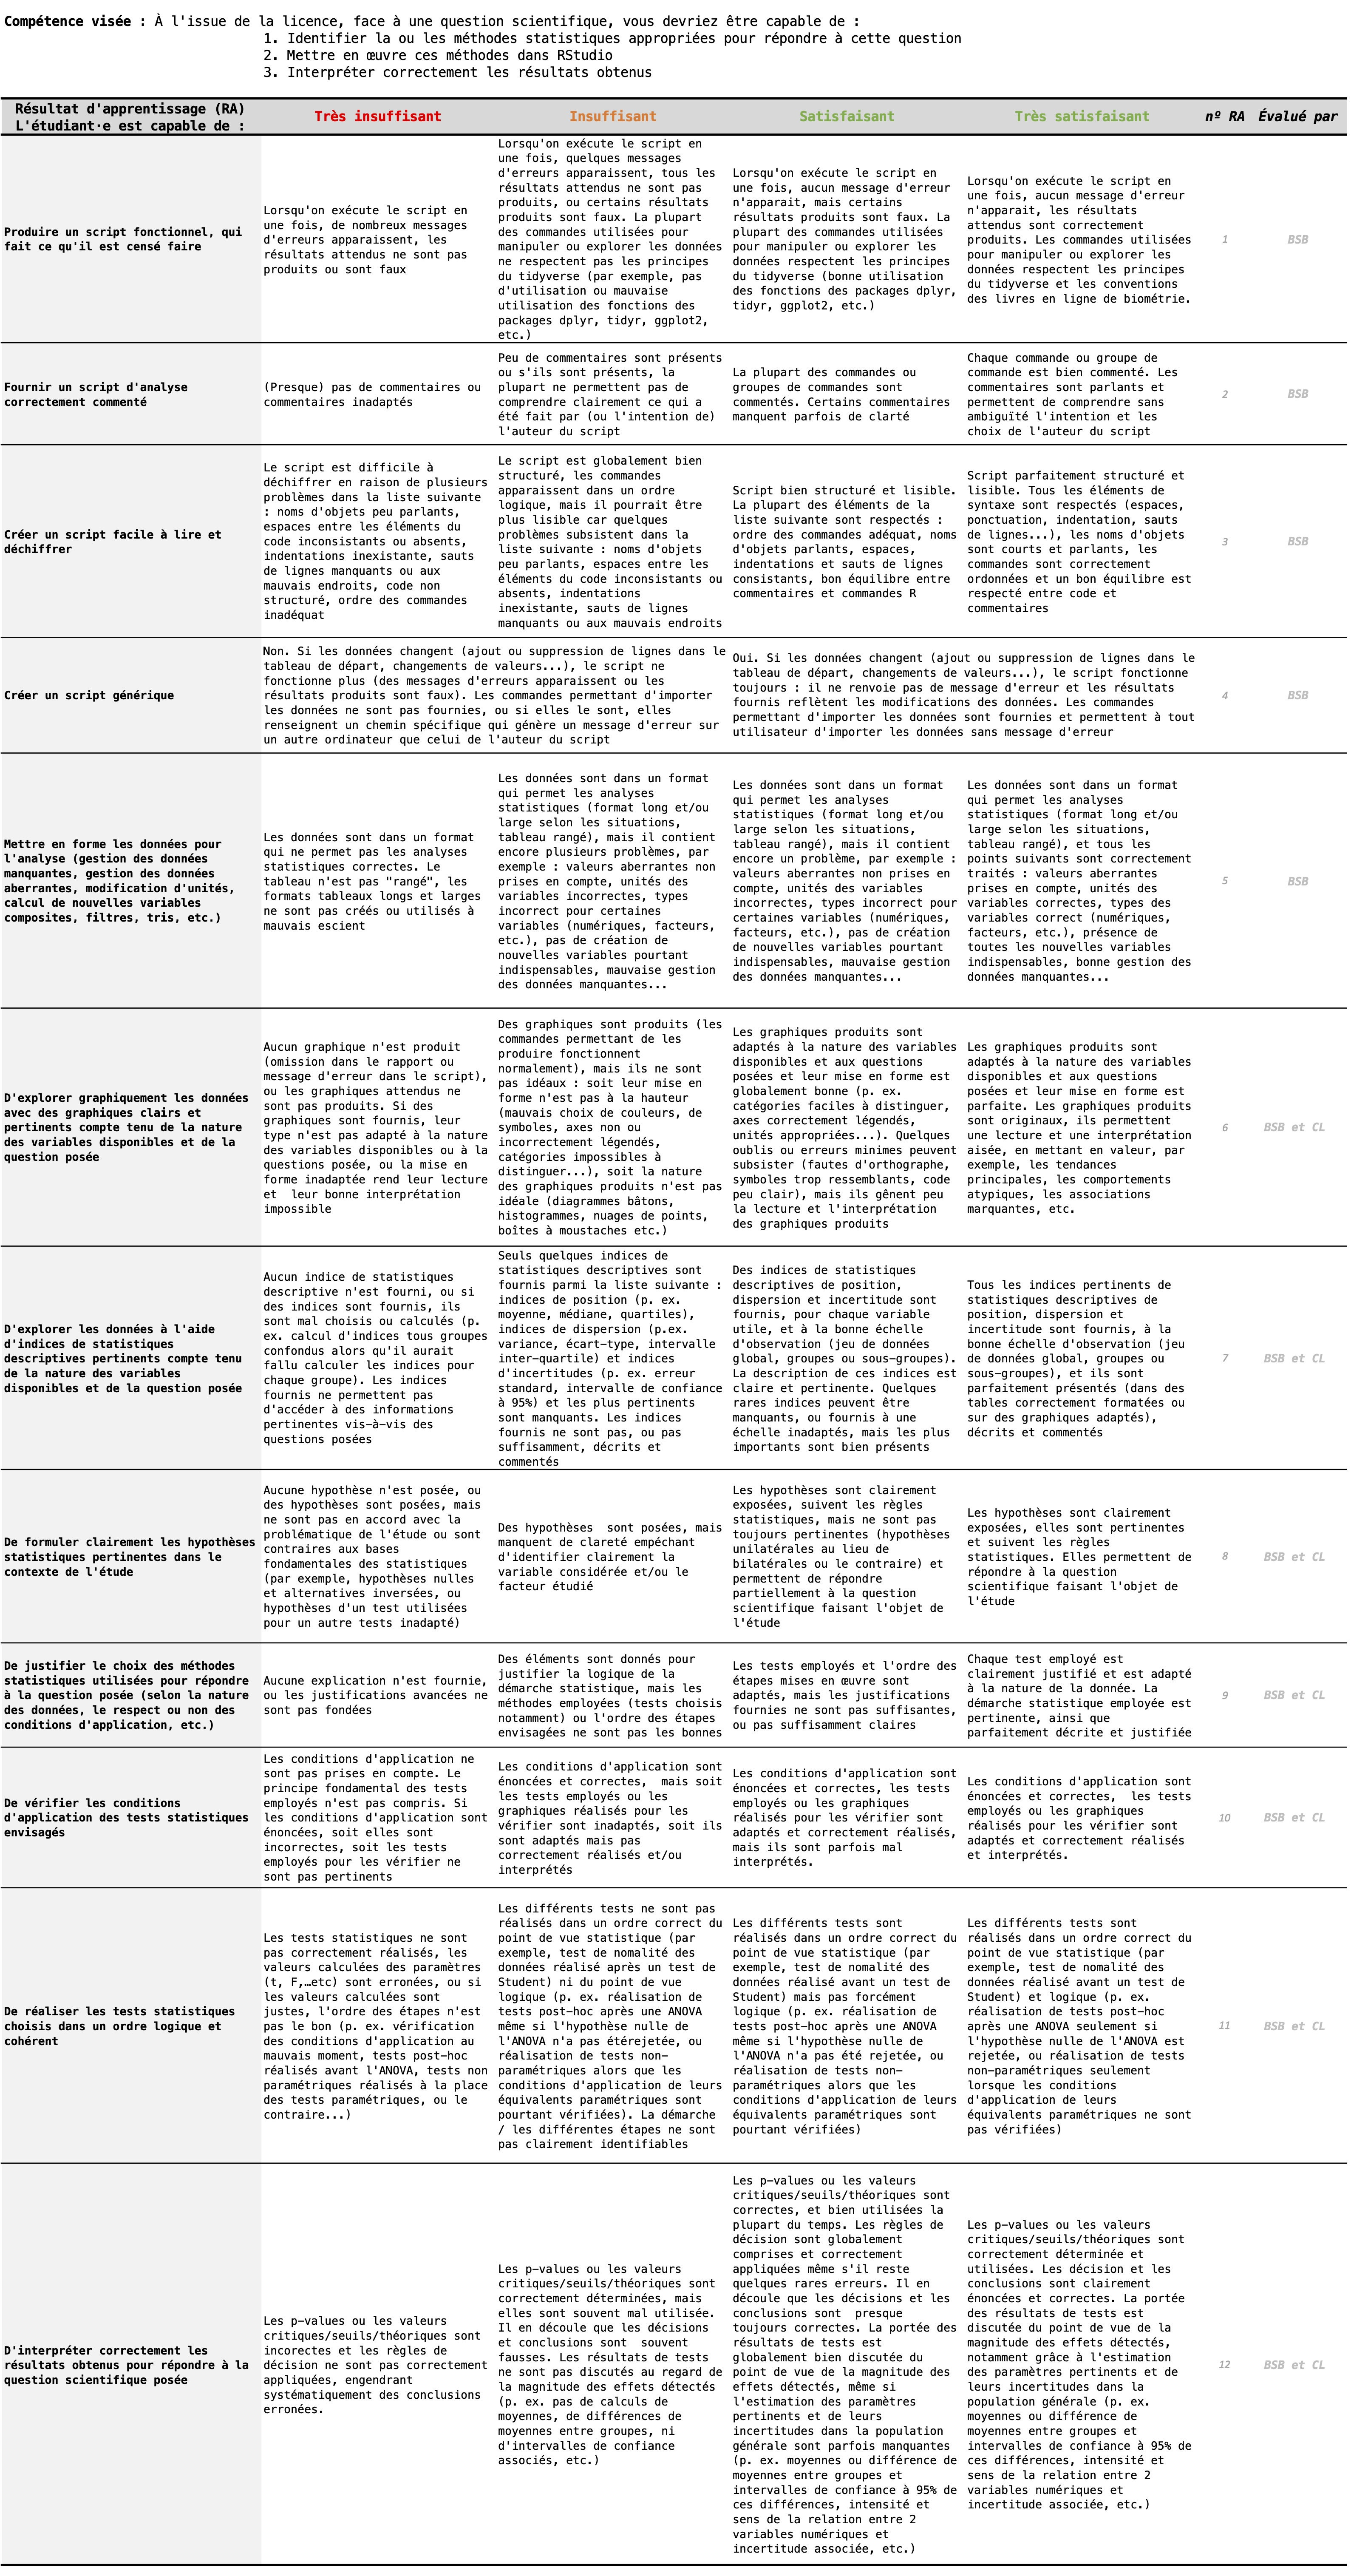
\includegraphics[keepaspectratio]{images/Grille.jpg}}

\section*{Licence}\label{licence}
\addcontentsline{toc}{section}{Licence}

\markright{Licence}

Ce livre est ligne est sous licence Creative Commons
(\href{https://creativecommons.org/licenses/by-nc-nd/4.0/deed.fr}{CC
BY-NC-ND 4.0})

\href{https://creativecommons.org/licenses/by-nc-nd/4.0/deed.fr}{\begin{center}
\pandocbounded{
\includegraphics[keepaspectratio]{images/cc_licence.png}}
\end{center}
}

Vous êtes autorisé à partager, copier, distribuer et communiquer ce
matériel par tous moyens et sous tous formats, tant que les conditions
suivantes sont respectées :

{\faIcon{creative-commons-by}} \textbf{Attribution} : vous devez
créditer ce travail (donc citer son auteur), fournir un lien vers ce
livre en ligne, intégrer un lien vers la licence Creative Commons et
indiquer si des modifications du contenu original ont été effectuées.
Vous devez indiquer ces informations par tous les moyens raisonnables,
sans toutefois suggérer que l'auteur vous soutient ou soutient la façon
dont vous avez utilisé son travail.

{\faIcon{creative-commons-nc-eu}} \textbf{Pas d'Utilisation Commerciale}
: vous n'êtes pas autorisé à faire un usage commercial de cet ouvrage,
ni de tout ou partie du matériel le composant. Cela comprend évidemment
la diffusion sur des plateformes de partage telles que studocu.com qui
tirent profit d'œuvres dont elles ne sont pas propriétaires, souvent à
l'insu des auteurs.

{\faIcon{creative-commons-nd}} \textbf{Pas de modifications} : dans le
cas où vous effectuez un remix, que vous transformez, ou créez à partir
du matériel composant l'ouvrage original, vous n'êtes pas autorisé à
distribuer ou mettre à disposition l'ouvrage modifié.

{\faIcon{unlock-alt}} \textbf{Pas de restrictions complémentaires} :
vous n'êtes pas autorisé à appliquer des conditions légales ou des
mesures techniques qui restreindraient légalement autrui à utiliser cet
ouvrage dans les conditions décrites par la licence.

\bookmarksetup{startatroot}

\chapter{Comparaison de la moyenne d'une population à une valeur
théorique}\label{sec-moy1}

\section{Pré-requis}\label{sec-packages}

Pour travailler dans de bonnes conditions, créez un nouveau dossier sur
votre ordinateur, créez un \texttt{Rproject} et un script dans ce
dossier, et travaillez systématiquement \textbf{dans votre script}, et
surtout pas directement dans la console. Consultez
\href{https://besibo.github.io/BiometrieS3/01-R-basics.html\#sec-code}{le
livre en ligne du semestre 3} si vous ne savez plus comment faire.

Dans ce chapitre, vous aurez besoin d'utiliser des packages spécifiques
et d'importer des données depuis des fichiers externes téléchargeables
directement depuis ce document. Les packages dont vous aurez besoin ici
et que vous devez donc charger en mémoire, sont :

\begin{itemize}
\tightlist
\item
  le \texttt{tidyverse} (Wickham 2023), qui comprend notamment le
  package \texttt{readr} (Wickham et al. 2024), pour importer facilement
  des fichiers \texttt{.csv} au format \texttt{tibble}, le package
  \texttt{dplyr} (Wickham et al. 2023), pour manipuler des tableaux, et
  le package \texttt{ggplot2} ({Wickham, Chang, et al.} 2025) pour les
  représentations graphiques.
\item
  \texttt{skimr} (Waring et al. 2022), qui permet de calculer des
  résumés de données très informatifs.
\end{itemize}

\begin{Shaded}
\begin{Highlighting}[]
\FunctionTok{library}\NormalTok{(tidyverse)}
\FunctionTok{library}\NormalTok{(skimr)}
\end{Highlighting}
\end{Shaded}

\begin{tcolorbox}[enhanced jigsaw, arc=.35mm, bottomrule=.15mm, bottomtitle=1mm, breakable, colback=white, colbacktitle=quarto-callout-warning-color!10!white, colframe=quarto-callout-warning-color-frame, coltitle=black, left=2mm, leftrule=.75mm, opacityback=0, opacitybacktitle=0.6, rightrule=.15mm, title=\textcolor{quarto-callout-warning-color}{\faExclamationTriangle}\hspace{0.5em}{Important}, titlerule=0mm, toprule=.15mm, toptitle=1mm]

Même si vous avez déjà installé le \texttt{tidyverse} ou \texttt{dplyr}
au semestre précédent, ré-installez \texttt{dplyr} avec
\texttt{install.packages("dplyr")}. Ce package a en effet été mis à jour
récemment, et nous aurons d'une version récente (\textgreater{} v1.1.0).
Chargez-le ensuite en mémoire avec \texttt{library(dplyr)}.

\end{tcolorbox}

\begin{tcolorbox}[enhanced jigsaw, arc=.35mm, bottomrule=.15mm, bottomtitle=1mm, breakable, colback=white, colbacktitle=quarto-callout-important-color!10!white, colframe=quarto-callout-important-color-frame, coltitle=black, left=2mm, leftrule=.75mm, opacityback=0, opacitybacktitle=0.6, rightrule=.15mm, title=\textcolor{quarto-callout-important-color}{\faExclamation}\hspace{0.5em}{Attention}, titlerule=0mm, toprule=.15mm, toptitle=1mm]

Pensez à installer tous les packages listés ci-dessous avant de les
charger en mémoire si vous ne l'avez pas déjà fait. Si vous ne savez
plus comment faire, consultez d'urgence
\href{https://besibo.github.io/BiometrieS3/01-R-basics.html\#sec-packages}{la
section dédiée aux packages dans le livre en ligne de Biométrie du
semestre 3}.

\end{tcolorbox}

Vous aurez également besoin des jeux de données suivants :

\begin{itemize}
\tightlist
\item
  \href{data/Temperature.csv}{\texttt{Temperature.csv}}
\item
  \href{data/Temperature2.csv}{\texttt{Temperature2.csv}}
\end{itemize}

Enfin, je spécifie ici une fois pour toutes le thème que j'utiliserai
pour tous les graphiques de ce chapitre. Libre à vous de choisir un
thème différent ou de vous contenter du thème proposé par défaut :

\begin{Shaded}
\begin{Highlighting}[]
\FunctionTok{theme\_set}\NormalTok{(}\FunctionTok{theme\_bw}\NormalTok{())}
\end{Highlighting}
\end{Shaded}

\section{Contexte}\label{contexte}

On s'intéresse ici à la température corporelle des adultes en bonne
santé. On souhaite examiner la croyance populaire qui veut que cette
température vaut en moyenne 37ºC. Pour le vérifier, on dispose d'un
échantillon de 25 adultes en bonne santé choisis au hasard parmi la
population américaine et dont on a mesuré la température. Comme pour
toute étude statistique, les étapes que nous allons devoir suivre sont
les suivantes (dans l'ordre) :

\begin{enumerate}
\def\labelenumi{\arabic{enumi}.}
\tightlist
\item
  Importer les données dans \texttt{RStudio}, les examiner et
  éventuellement les (re)mettre en forme si besoin.
\item
  Faire une première exploration des données, grâce au calcul d'indices
  de statistiques descriptives d'une part, et de représentations
  graphiques d'autre part.
\item
  Réaliser un test d'hypothèses en respectant la procédure adéquate (en
  particulier, la vérification des conditions d'application).
\end{enumerate}

C'est donc ce que nous allons faire dans les sections suivantes.

\begin{tcolorbox}[enhanced jigsaw, arc=.35mm, bottomrule=.15mm, bottomtitle=1mm, breakable, colback=white, colbacktitle=quarto-callout-important-color!10!white, colframe=quarto-callout-important-color-frame, coltitle=black, left=2mm, leftrule=.75mm, opacityback=0, opacitybacktitle=0.6, rightrule=.15mm, title=\textcolor{quarto-callout-important-color}{\faExclamation}\hspace{0.5em}{À retenir !}, titlerule=0mm, toprule=.15mm, toptitle=1mm]

Avant de se lancer dans les tests d'hypothèses, il est \textbf{toujours
indispensable} d'examiner les données dont on dispose à l'aide, d'une
part de statistiques descriptives numériques, et d'autres part, de
graphiques exploratoires.

Nous avons vu au cours des semestres précédents quels indices
statistiques il peut être utile de calculer
(\href{https://besibo.github.io/BiometrieS4/01-dispersion.html}{dans le
livre en ligne du semestre 4}) et quelles représentations graphiques il
peut être utile de réaliser
(\href{https://besibo.github.io/BiometrieS3/03-visualization.html}{dans
le livre en ligne du semestre 3}) afin de pouvoir se lancer dans des
tests d'hypothèses sans risquer de grossières erreurs. N'hésitez pas à
cliquer sur ces liens pour vous rafraîchir la mémoire !

\end{tcolorbox}

\section{Importation et mise en forme des
données}\label{importation-et-mise-en-forme-des-donnuxe9es}

Nous allons travailler ici sur les données contenues dans le fichier
\href{data/Temperature.csv}{\texttt{Temperature.csv}}. Téléchargez ces
données dans votre répertoire de travail (attention : ne les ouvrez pas
avec Excel !), puis importez les données dans \texttt{RStudio} grâce à
l'assistant d'importation. Si vous ne savez plus comment faire,
consultez
\href{https://besibo.github.io/BiometrieS3/04-DataWrangling.html\#plaintext}{la
section dédiée à l'importation des données dans le livre en ligne de
Biométrie du semestre 3}

Vous stockerez les données dans un objet que vous nommerez
\texttt{Temperature}. Après l'importation, tapez son nom dans la console
de \texttt{RStudio} et vérifiez que vous obtenez bien exactement ce
résultat :

\begin{Shaded}
\begin{Highlighting}[]
\NormalTok{Temperature}
\end{Highlighting}
\end{Shaded}

\begin{verbatim}
# A tibble: 25 x 2
   individual temperature
        <dbl>       <dbl>
 1          1        98.4
 2          2        98.6
 3          3        97.8
 4          4        98.8
 5          5        97.9
 6          6        99  
 7          7        98.2
 8          8        98.8
 9          9        98.8
10         10        99  
# i 15 more rows
\end{verbatim}

La première chose à faire quand on travaille avec des données inconnues,
c'est d'examiner les données brutes. Ici, les données sont importées au
format \texttt{tibble}, donc seules les premières lignes sont visibles.
Pour visualiser l'ensemble du tableau, utilisez la fonction
\texttt{View()} (avec un \texttt{V} majuscule) ou, si vous avez mis en
mémoire le \texttt{tidyverse}, la fonction \texttt{view()} (sans
majuscule) :

\begin{Shaded}
\begin{Highlighting}[]
\FunctionTok{View}\NormalTok{(Temperature)}
\end{Highlighting}
\end{Shaded}

Cette commande ouvre un nouvel onglet présentant les données dans un
tableur simplifié, en lecture seule. On constate ici 2 choses que nous
allons modifier :

\begin{enumerate}
\def\labelenumi{\arabic{enumi}.}
\tightlist
\item
  la première colonne, intitulée \texttt{individual}, n'est pas
  véritablement une variable. Cette colonne ne contient qu'un
  identifiant sans intérêt pour notre étude et est en fait identique au
  numéro de ligne. Nous allons donc supprimer cette colonne.
\item
  les températures sont exprimées en degrés Fahrenheit, ce qui rend leur
  lecture difficile pour nous qui sommes habitués à utiliser le système
  métrique et les degrés Celsius. Nous allons donc convertir les
  températures en degrés Celsius grâce à la formule suivante :
\end{enumerate}

\[ºC = \frac{ºF - 32}{1.8}\]

\begin{Shaded}
\begin{Highlighting}[]
\NormalTok{Temp\_clean }\OtherTok{\textless{}{-}}\NormalTok{ Temperature }\SpecialCharTok{|\textgreater{}}
  \FunctionTok{select}\NormalTok{(}\SpecialCharTok{{-}}\NormalTok{individual) }\SpecialCharTok{|\textgreater{}}      \CommentTok{\# Suppression de la colonne \textasciigrave{}individual\textasciigrave{}}
  \FunctionTok{mutate}\NormalTok{(                      }\CommentTok{\# Transformation des températures en ºCelsius}
    \AttributeTok{temperature =}\NormalTok{ (temperature }\SpecialCharTok{{-}} \DecValTok{32}\NormalTok{) }\SpecialCharTok{/} \FloatTok{1.8}
\NormalTok{    )}

\NormalTok{Temp\_clean}
\end{Highlighting}
\end{Shaded}

\begin{verbatim}
# A tibble: 25 x 1
   temperature
         <dbl>
 1        36.9
 2        37  
 3        36.6
 4        37.1
 5        36.6
 6        37.2
 7        36.8
 8        37.1
 9        37.1
10        37.2
# i 15 more rows
\end{verbatim}

Il nous est maintenant possible d'examiner à nouveau les données avec la
fonction \texttt{View()}. Avec des valeurs de températures comprises
entre 36.3ºC et 37.8ºC, il n'y a visiblement pas de données aberrantes.

Examiner les données brutes est donc la première chose que vous devriez
prendre l'habitude de faire, et ce de façon systématique, car cela
permet de repérer :

\begin{itemize}
\tightlist
\item
  La nature des variables présentes.
\item
  Les variables inutiles qui pourront être supprimées ou négligées.
\item
  Les unités des variables utiles, afin de pouvoir les convertir si
  nécessaire.
\item
  Les valeurs manquantes, atypiques ou aberrantes qui demanderont
  toujours une attention particulière.
\end{itemize}

Maintenant que l'examen préliminaire des données est réalisé, on peut
passer au calcul des statistiques descriptives.

\section{Exploration statistique des données}\label{sec-eda}

\subsection{Position et dispersion}\label{position-et-dispersion}

On s'intéresse ici au calcul de grandeurs statistiques nous apportant
des renseignements sur la \textbf{position} et la \textbf{dispersion}
des valeurs de l'échantillon. Les questions auxquelles on tente de
répondre à ce stade sont les suivantes :

\begin{itemize}
\tightlist
\item
  Quelle est la tendance centrale (moyenne ou médiane) ?
\item
  Quelle est la dispersion des valeurs autour de la tendance centrale
  (écart-type, variance, intervalle interquartile\ldots) ?
\end{itemize}

Pour répondre à ces questions, on peut faire appel à de multiples
fonctions déjà présentées
\href{https://besibo.github.io/BiometrieS4/01-dispersion.html}{dans le
livre en ligne du semestre 4}. Par exemple la fonction
\texttt{summarise()}, en conjonction avec les fonctions \texttt{mean()},
\texttt{median()}, \texttt{sd()}, \texttt{var()}, \texttt{min()},
\texttt{max()} ou \texttt{quantile()}, ou les fonctions
\texttt{summary()} ou \texttt{skim()} (du package \texttt{skimr}).

Je prends ici un exemple simple, mais n'hésitez pas à expérimenter avec
les méthodes décrites dans le livre en ligne du semestre 4.

\begin{Shaded}
\begin{Highlighting}[]
\FunctionTok{summary}\NormalTok{(Temp\_clean)}
\end{Highlighting}
\end{Shaded}

\begin{verbatim}
  temperature   
 Min.   :36.33  
 1st Qu.:36.67  
 Median :37.00  
 Mean   :36.96  
 3rd Qu.:37.22  
 Max.   :37.78  
\end{verbatim}

On constate ici que la moyenne et la médiane sont très proches. La
distribution des températures doit donc être à peut près symétrique,
avec à peu près autant de valeurs au-dessus que de valeurs en dessous de
la moyenne. Les premier et troisième quartiles sont à peu près aussi
éloignés de la médiane l'un que l'autre, ce qui confirme l'apparente
symétrie du jeu de données de part et d'autre de la tendance centrale.

La moyenne observée dans l'échantillon vaut 36.96ºC, ce qui est très
proche de la moyenne théorique de 37ºC.

Une autre fonction utile est la fonction \texttt{IQR()}, qui renvoie
l'étendue de l'intervalle interquartile (la valeur du troisième quartile
moins la valeur de premier quartile) :

\begin{Shaded}
\begin{Highlighting}[]
\NormalTok{Temp\_clean }\SpecialCharTok{|\textgreater{}}
  \FunctionTok{summarise}\NormalTok{(}\AttributeTok{IQ\_range =} \FunctionTok{IQR}\NormalTok{(temperature))}
\end{Highlighting}
\end{Shaded}

\begin{verbatim}
# A tibble: 1 x 1
  IQ_range
     <dbl>
1    0.556
\end{verbatim}

On constate ici que l'intervalle interquartile a une largeur de 0.56ºC.
Cela signifie que les 50\% des températures les plus centrales de
l'échantillon sont situées dans un intervalle d'environ un demi-degré
Celsius autour de la médiane.

Enfin, pour obtenir des informations complémentaires, on peut utiliser
la fonction \texttt{skim()} du package \texttt{skimr} :

\begin{Shaded}
\begin{Highlighting}[]
\FunctionTok{skim}\NormalTok{(Temp\_clean)}
\end{Highlighting}
\end{Shaded}

\begin{verbatim}
-- Data Summary ------------------------
                           Values    
Name                       Temp_clean
Number of rows             25        
Number of columns          1         
_______________________              
Column type frequency:               
  numeric                  1         
________________________             
Group variables            None      

-- Variable type: numeric ------------------------------------------------------
  skim_variable n_missing complete_rate mean    sd   p0  p25 p50  p75 p100 hist 
1 temperature           0             1 37.0 0.377 36.3 36.7  37 37.2 37.8 ▇▇▇▇▂
\end{verbatim}

Tout comme \texttt{summary()}, la fonction \texttt{skim()} renvoie les
valeurs minimales et maximales, les premiers et troisièmes quartiles
ainsi que la moyenne et la médiane. Elle nous indique en outre la valeur
de l'écart-type de l'échantillon, ainsi que le nombre d'observations et
le nombre de données manquantes. Enfin, elle fournit un histogramme très
simplifié et sans échelle. Cet histogramme nous permet de nous faire une
première idée de la distribution des données et est particulièrement
utile pour comparer rapidement un grand nombre de distributions quand il
y a plusieurs catégories dans les données (ce qui n'est pas le cas ici).

Outre ces 3 fonctions (\texttt{summary()}, \texttt{IQR()}, et
\texttt{skim()}), il est bien sûr possible de calculer toutes ces
valeurs manuellement si besoin :

\begin{itemize}
\tightlist
\item
  \texttt{mean()} permet de calculer la moyenne.
\item
  \texttt{median()} permet de calculer la médiane.
\item
  \texttt{min()} et \texttt{max()} permettent de calculer les valeurs
  minimales et maximales respectivement.
\item
  \texttt{quantile()} permet de calculer les quartiles.
\item
  \texttt{sd()} permet de calculer l'écart-type.
\item
  \texttt{var()} permet de calculer la variance.
\item
  \texttt{n()} permet de compter le nombre d'observations.
\end{itemize}

Toutes ces fonctions prennent seulement un vecteur en guise d'argument.
Il faut donc procéder comme avec \texttt{IQR()} pour les utiliser, en
les intégrant à l'intérieur de la fonction \texttt{summarise()}. Par
exemple, pour calculer la variance, on peut taper :

\begin{Shaded}
\begin{Highlighting}[]
\NormalTok{Temp\_clean }\SpecialCharTok{|\textgreater{}} 
  \FunctionTok{summarise}\NormalTok{(}\AttributeTok{variance =} \FunctionTok{var}\NormalTok{(temperature))}
\end{Highlighting}
\end{Shaded}

\begin{verbatim}
# A tibble: 1 x 1
  variance
     <dbl>
1    0.142
\end{verbatim}

ou :

\begin{Shaded}
\begin{Highlighting}[]
\NormalTok{Temp\_clean }\SpecialCharTok{|\textgreater{}}
  \FunctionTok{pull}\NormalTok{(temperature) }\SpecialCharTok{|\textgreater{}}
  \FunctionTok{var}\NormalTok{()}
\end{Highlighting}
\end{Shaded}

\begin{verbatim}
[1] 0.1417901
\end{verbatim}

ou encore :

\begin{Shaded}
\begin{Highlighting}[]
\FunctionTok{var}\NormalTok{(Temp\_clean}\SpecialCharTok{$}\NormalTok{temperature)}
\end{Highlighting}
\end{Shaded}

\begin{verbatim}
[1] 0.1417901
\end{verbatim}

À vous d'utiliser la syntaxe qui vous semble la plus simple.

\subsection{Incertitude}\label{sec-ic95}

Outre les informations de position et de dispersion, nous avons vu
\href{https://besibo.github.io/BiometrieS4/02-incertitude.html\#la-notion-dincertitude}{au
semestre 4} qu'il était également important d'avoir une idée de
l'\textbf{incertitude} associée aux estimations de tendance centrale
(erreur standard ou intervalle de confiance de la moyenne ou médiane).
Ici, nous allons donc calculer l'intervalle de confiance à 95\% de la
moyenne. Si vous ne savez plus comment faire, ou que vous ne comprenez
pas le code ci-dessous, consultez
\href{https://besibo.github.io/BiometrieS4/02-incertitude.html\#sec-confint}{le
livre en ligne du semestre 4} :

\begin{Shaded}
\begin{Highlighting}[]
\NormalTok{Temp\_clean }\SpecialCharTok{|\textgreater{}} 
  \FunctionTok{reframe}\NormalTok{(}\FunctionTok{mean\_cl\_normal}\NormalTok{(temperature))}
\end{Highlighting}
\end{Shaded}

\begin{verbatim}
# A tibble: 1 x 3
      y  ymin  ymax
  <dbl> <dbl> <dbl>
1  37.0  36.8  37.1
\end{verbatim}

On constate ici que les bornes inférieure (36.8ºC) et supérieure
(37.1ºC) de l'intervalle de confiance à 95\% de la moyenne sont proches
de la valeur de moyenne de l'échantillon. Dans la population générale,
la moyenne de la température corporelle chez les adultes en bonne santé
a de bonnes chances de se trouver quelque part entre 36.8ºC et 37.1ºC.
Autrement dit, si la température corporelle des adultes en bonne santé
n'est pas exactement de 37ºC, l'écart à cette valeur théorique ne doit
pas être très important.

\section{Exploration graphique des données}\label{sec-edagraph}

Ici, puisque nous ne disposons que d'une unique variable numérique et
que nous n'avons donc qu'un unique groupe, les représentations
graphiques que nous allons réaliser doivent nous permettre d'examiner la
\textbf{distribution des données}. Pour cela, nous pouvons réaliser soit
un histogramme, soit un diagramme de densité.

\subsection{Histogramme}\label{histogramme}

Voilà comment produire un histogramme de qualité pour les données de
températures :

\begin{Shaded}
\begin{Highlighting}[]
\NormalTok{Temp\_clean }\SpecialCharTok{|\textgreater{}}
  \FunctionTok{ggplot}\NormalTok{(}\FunctionTok{aes}\NormalTok{(}\AttributeTok{x =}\NormalTok{ temperature)) }\SpecialCharTok{+}
  \FunctionTok{geom\_histogram}\NormalTok{(}\AttributeTok{bins =} \DecValTok{10}\NormalTok{, }\AttributeTok{fill =} \StringTok{"firebrick2"}\NormalTok{, }\AttributeTok{color =} \StringTok{"grey20"}\NormalTok{, }
                 \AttributeTok{alpha =} \FloatTok{0.5}\NormalTok{) }\SpecialCharTok{+}
  \FunctionTok{geom\_rug}\NormalTok{() }\SpecialCharTok{+}
  \FunctionTok{labs}\NormalTok{(}\AttributeTok{x =} \StringTok{"Température (ºC)"}\NormalTok{,}
       \AttributeTok{y =} \StringTok{"Fréquence"}\NormalTok{,}
       \AttributeTok{title =} \StringTok{"Distribution des températures corporelles"}\NormalTok{,}
       \AttributeTok{subtitle =} \StringTok{"n = 25 adultes en bonne santé"}\NormalTok{)}
\end{Highlighting}
\end{Shaded}

\pandocbounded{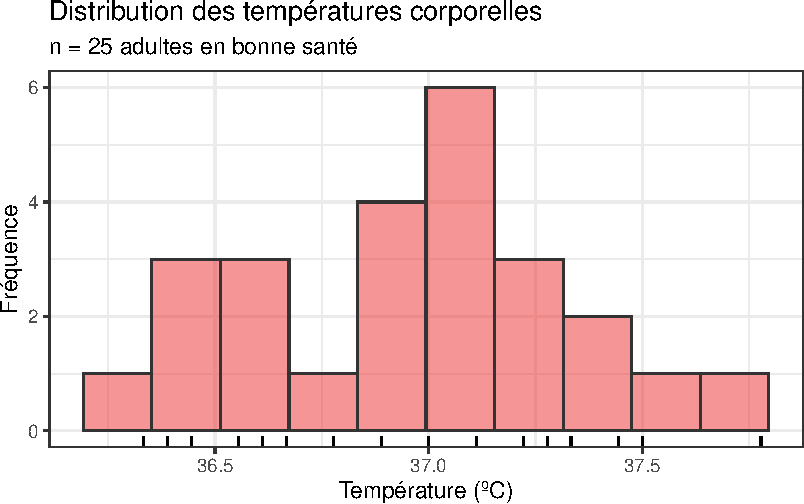
\includegraphics[keepaspectratio]{01-OneSampleTests_files/figure-pdf/unnamed-chunk-14-1.pdf}}

Si vous ne vous rappelez-plus ce qu'est un histogramme ou comment le
faire, ou la signification de l'argument \texttt{bins}, relisez
\href{https://besibo.github.io/DA/viz.html\#histogram}{la section
consacrée aux histogrammes} du livre en ligne de Biométrie du semestre
3. Notez que j'ai ajouté une couleur de remplissage et de la
transparence pour rendre le graphique plus facile à lire. J'ai également
spécifié des titres pour les axes (en précisant l'unité de la variable
numérique dont on représente la distribution) ainsi que le titre (et
sous-titre) du graphique, qui précise ce qu'on a sous les yeux et la
taille de l'échantillon. Il n'est pas toujours nécessaire de spécifier
le titre (et le sous-titre) de cette façon : lorsque vous intégrez des
graphiques dans un compte-rendu ou un rapport, le titre est en général
précisé sous la figure, au début d'une légende qui la décrit. Enfin,
j'ai ajouté \texttt{geom\_rug()} pour faire apparaître sous le
graphique, le long de l'axe des \texttt{x}, la position des données
observées. Cela permet de visualiser les données brutes, et peut donc
permettre de mieux comprendre pourquoi un histogramme présente telle ou
telle forme.

Ici, la forme de ce l'histogramme est assez proche de celle présentée
plus tôt par l'histogramme très simplifié produit par la fonction
\texttt{skim()}. Cet histogramme nous apprend qu'en dehors d'un ``trou''
autour de la température 36.75ºC, la distribution des données est proche
d'une courbe en cloche. Il y a fort à parier qu'un test de normalité
conclurait à la normalité des données de cet échantillon. C'est ce que
nous verrons dans la Section~\ref{sec-norm}.

\subsection{Diagramme de densité}\label{diagramme-de-densituxe9}

Une autre façon de visualiser la distribution d'une variable numérique
est de produire un graphique de densité. Il a l'avantage d'éviter à
l'utilisateur d'avoir à choisir une valeur pour l'argument \texttt{bin}
de la fonction \texttt{geom\_histogram()}, mais il a l'inconvénient de
présenter une échelle plus difficile à comprendre pour l'axe des
ordonnées :

\begin{Shaded}
\begin{Highlighting}[]
\NormalTok{Temp\_clean }\SpecialCharTok{|\textgreater{}}
  \FunctionTok{ggplot}\NormalTok{(}\FunctionTok{aes}\NormalTok{(}\AttributeTok{x =}\NormalTok{ temperature)) }\SpecialCharTok{+}
  \FunctionTok{geom\_density}\NormalTok{(}\AttributeTok{fill =} \StringTok{"firebrick2"}\NormalTok{, }\AttributeTok{alpha =} \FloatTok{0.5}\NormalTok{) }\SpecialCharTok{+}
  \FunctionTok{geom\_rug}\NormalTok{() }\SpecialCharTok{+}
  \FunctionTok{labs}\NormalTok{(}\AttributeTok{x =} \StringTok{"Température (ºC)"}\NormalTok{,}
       \AttributeTok{y =} \StringTok{"Densité"}\NormalTok{,}
       \AttributeTok{title =} \StringTok{"Distribution des températures corporelles"}\NormalTok{,}
       \AttributeTok{subtitle =} \StringTok{"n = 25 adultes en bonne santé"}\NormalTok{)}
\end{Highlighting}
\end{Shaded}

\pandocbounded{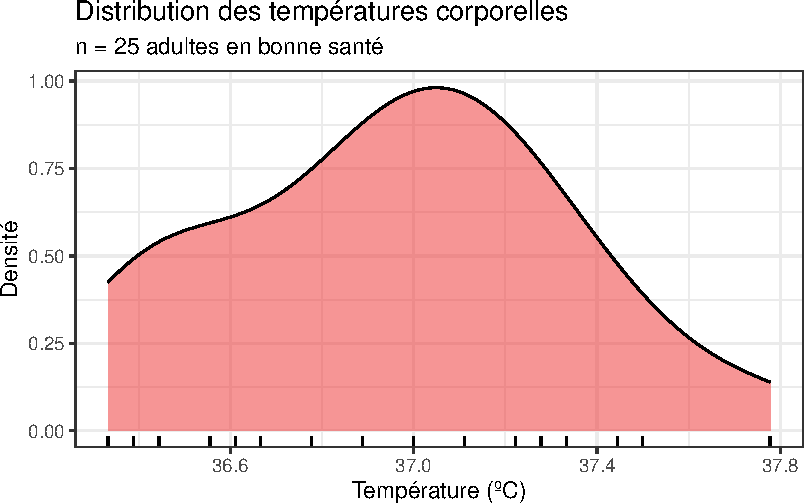
\includegraphics[keepaspectratio]{01-OneSampleTests_files/figure-pdf/unnamed-chunk-15-1.pdf}}

Les informations apportées par ce graphique sont cohérentes avec celle
de l'histogramme :

\begin{itemize}
\tightlist
\item
  les températures les plus fréquemment observées dans notre échantillon
  de 25 adultes en bonne santé se situent légèrement au dessus de 37ºC.
  Il s'agit d'une information concernant la \textbf{position} des
  données (c'est-à-dire où se trouve le pic de la distribution sur l'axe
  des \texttt{x})
\item
  les températures observées ont une distribution qui ressemble à peu
  près à une courbe en cloche, avec des valeurs comprises entre 36.4ºC
  et 37.8ºC environ. La symétrie de part et d'autre du pic n'est pas
  parfaite, mais elle reste bonne. Il s'agit d'informations concernant
  la forme de la distribution et la \textbf{dispersion} des données.
\end{itemize}

\begin{tcolorbox}[enhanced jigsaw, arc=.35mm, bottomrule=.15mm, bottomtitle=1mm, breakable, colback=white, colbacktitle=quarto-callout-note-color!10!white, colframe=quarto-callout-note-color-frame, coltitle=black, left=2mm, leftrule=.75mm, opacityback=0, opacitybacktitle=0.6, rightrule=.15mm, title=\textcolor{quarto-callout-note-color}{\faInfo}\hspace{0.5em}{Bilan des analyses préliminaires}, titlerule=0mm, toprule=.15mm, toptitle=1mm]

Suite à l'exploration statistique et graphique des données de
températures, voilà ce qu'on retient :

\begin{enumerate}
\def\labelenumi{\arabic{enumi}.}
\tightlist
\item
  Il n'y a visiblement pas de données aberrantes.
\item
  La distribution des données semble suivre à peu près la loi Normale.
\item
  La médiane et la moyenne sont très proches de 37ºC. Un test devrait
  donc arriver à la conclusion que la température corporelle des adultes
  n'est pas significativement différente de 37ºC.
\item
  La largeur de l'intervalle de confiance à 95\% semble faible, ce qui
  indique une incertitude relativement faible. Si la température réelle
  des adultes en bonne santé n'est pas exactement de 37ºC, elle ne
  devrait pas en être très éloignée (quelques dixièmes de degrés Celsuis
  au plus).
\end{enumerate}

\end{tcolorbox}

\section{Le test paramétrique}\label{le-test-paramuxe9trique}

Le test permettant de comparer la moyenne \(\mu\) d'une population à une
valeur théorique, fixée par l'utilisateur, est le \textbf{test de
Student à un échantillon}. Il permet de répondre à la question suivante
:

\begin{quote}
Les données observés dans l'échantillon dont je dispose sont-elles
compatibles avec l'hypothèse que la moyenne \(\mu\) de la population
dont est issu mon échantillon vaut \texttt{XXX} ?
\end{quote}

avec \texttt{XXX}, une valeur d'intérêt spécifiée par l'utilisateur. Il
s'agit d'un test paramétrique très puissant. Comme tous les tests
paramétriques, certaines conditions d'application doivent être vérifiées
avant de pouvoir l'appliquer.

\begin{tcolorbox}[enhanced jigsaw, arc=.35mm, bottomrule=.15mm, bottomtitle=1mm, breakable, colback=white, colbacktitle=quarto-callout-important-color!10!white, colframe=quarto-callout-important-color-frame, coltitle=black, left=2mm, leftrule=.75mm, opacityback=0, opacitybacktitle=0.6, rightrule=.15mm, title=\textcolor{quarto-callout-important-color}{\faExclamation}\hspace{0.5em}{Important}, titlerule=0mm, toprule=.15mm, toptitle=1mm]

Comme pour tous les tests statistiques que nous allons réaliser lors de
ces séances de TP et TEA, nous devrons commencer par \textbf{spécifier
les hypothèses} nulles et alternatives de chaque test, ainsi que la
\textbf{valeur du seuil} \(\alpha\) que nous allons utiliser. À moins
d'avoir une bonne raison de faire autrement, on utilise presque toujours
le seuil \(\alpha = 0.05\) dans le domaine des sciences du vivant. C'est
donc ce seuil que nous utiliserons dans ce livre en ligne.

\end{tcolorbox}

\subsection{Conditions d'application}\label{sec-norm}

Les conditions d'application du test de Student à un échantillon sont
les suivantes :

\begin{enumerate}
\def\labelenumi{\arabic{enumi}.}
\tightlist
\item
  Les données de l'échantillon sont issues d'un \textbf{échantillonnage
  aléatoire} au sein de la population générale. Cette condition est
  partagée par toutes les méthodes que nous verrons dans ces TP. En
  l'absence d'informations sur la façon dont l'échantillonnage a été
  réalisé, on considère que cette condition est remplie. Il n'y a pas de
  moyen statistique de le vérifier, cela fait uniquement référence à la
  stratégie d'échantillonnage déployée et à la rigueur de la procédure
  mise en œuvre lors de l'acquisition des données.
\item
  La variable étudiée doit suivre une \textbf{distribution Normale} dans
  la population générale. Nous allons vérifier cette condition
  d'application avec un \textbf{test de normalité de Shapiro-Wilk}.
\end{enumerate}

Pour un test de normalité, les hypothèses seront toujours les suivantes
:

\begin{itemize}
\tightlist
\item
  H\(_0\) : la variable étudiée suit une distribution Normale dans la
  population générale.
\item
  H\(_1\) : la variable étudiée ne suit pas une distribution Normale
  dans la population générale.
\end{itemize}

Le test de Shapiro-Wilk se réalise de la façon suivante :

\begin{Shaded}
\begin{Highlighting}[]
\FunctionTok{shapiro.test}\NormalTok{(Temp\_clean}\SpecialCharTok{$}\NormalTok{temperature)}
\end{Highlighting}
\end{Shaded}

ou

\begin{Shaded}
\begin{Highlighting}[]
\NormalTok{Temp\_clean }\SpecialCharTok{|\textgreater{}}
  \FunctionTok{pull}\NormalTok{(temperature) }\SpecialCharTok{|\textgreater{}}
  \FunctionTok{shapiro.test}\NormalTok{()}
\end{Highlighting}
\end{Shaded}

\begin{verbatim}

    Shapiro-Wilk normality test

data:  pull(Temp_clean, temperature)
W = 0.97216, p-value = 0.7001
\end{verbatim}

la fonction \texttt{pull()} permet d'extraire une colonne (ici
\texttt{temperature}) d'un tibble (ici \texttt{Temp\_clean}) et de la
transformer en vecteur.

\texttt{W} est la statistique du test. Elle permet à RStudio de calculer
la \emph{p}-value. Ici, \(p > \alpha\). On ne peut donc pas rejeter
l'hypothèse nulle de normalité : on ne peut pas exclure que dans la
population générale, la température suive bel et bien une distribution
Normale. Les conditions d'application du test de Student sont bien
vérifiées.

\begin{tcolorbox}[enhanced jigsaw, arc=.35mm, bottomrule=.15mm, bottomtitle=1mm, breakable, colback=white, colbacktitle=quarto-callout-warning-color!10!white, colframe=quarto-callout-warning-color-frame, coltitle=black, left=2mm, leftrule=.75mm, opacityback=0, opacitybacktitle=0.6, rightrule=.15mm, title=\textcolor{quarto-callout-warning-color}{\faExclamationTriangle}\hspace{0.5em}{Tests et décision : rappel de cours}, titlerule=0mm, toprule=.15mm, toptitle=1mm]

À l'issue d'un tests statistique, la décision finale est toujours prise
par rapport à l'hypothèse nulle (\(H_0\)) :

\begin{itemize}
\tightlist
\item
  Si la \(p-\)value du test est supérieure ou égale à \(\alpha\), on dit
  qu'on ne peut pas rejeter l'hypothèse nulle \(H_0\). Attention, on ne
  dit jamais que ``\(H_0\) est vraie'', car il est impossible de le
  vérifier avec une certitude absolue. Toutefois, les données observées
  (celles de notre échantillon), sont compatibles avec l'hypothèse nulle
  que nous avons formulée, jusqu'à preuve du contraire.
\item
  Si la \(p-\)value du test est inférieure à \(\alpha\), on dit qu'on
  rejette l'hypothèse nulle au seuil \(\alpha\). Autrement dit, les
  données observées ne sont pas compatibles avec l'hypothèse nulle. On
  accepte alors l'hypothèse alternative (\(H_A\)).
\end{itemize}

L'hypothèse nulle est toujours l'hypothèse la moins ``intéressante'',
celle pour laquelle ``il ne se passe rien de notable'' (par exemple :
``les données suivent la distribution Normale'', ou ``les moyennes sont
égales'').

\end{tcolorbox}

\subsection{\texorpdfstring{Signification de la
\(p-\)value}{Signification de la p-value}}\label{signification-de-la-p-value}

La \(p-\)value est une grandeur centrale en statistiques et elle est
souvent mal comprise et donc mal interprétée. Je prends donc le temps
ici d'expliquer ce qu'est la \(p-\)value et comment il faut la
comprendre.

\begin{tcolorbox}[enhanced jigsaw, arc=.35mm, bottomrule=.15mm, bottomtitle=1mm, breakable, colback=white, colbacktitle=quarto-callout-tip-color!10!white, colframe=quarto-callout-tip-color-frame, coltitle=black, left=2mm, leftrule=.75mm, opacityback=0, opacitybacktitle=0.6, rightrule=.15mm, title=\textcolor{quarto-callout-tip-color}{\faLightbulb}\hspace{0.5em}{Définition : la \(p-\)value}, titlerule=0mm, toprule=.15mm, toptitle=1mm]

La \(p-\)value d'un test statistique, c'est la probabilité, si \(H_0\)
est vraie, d'obtenir un effet au moins aussi extrême que celui qu'on a
observé dans l'échantillon, sous le seul effet du hasard.

\end{tcolorbox}

Ici, la \(p-\)value de notre test de Normalité de Shapiro-Wilk vaut
0.7101. Cela signifie que si les données suivent réellement la loi
Normale dans la population générale (donc si \(H_0\) est vraie), l'écart
à la Normalité que nous avons observé (ou un écart encore plus
important), peut être observé dans 70.1\% des cas. Autrement dit, si on
prélève un grand nombre d'échantillons de 25 adultes dans la population
générale et qu'on regarde à quoi ressemble la distribution des
températures dans chacun de ces échantillons, pour 70.1\% d'entre eux,
la distribution obtenue sera au moins aussi éloignée de la distribution
Normale que celle que nous avons observée ici.

Dans notre cas, l'écart entre la loi Normale et les données de notre
échantillon peut être visualisé de la façon suivante :

\pandocbounded{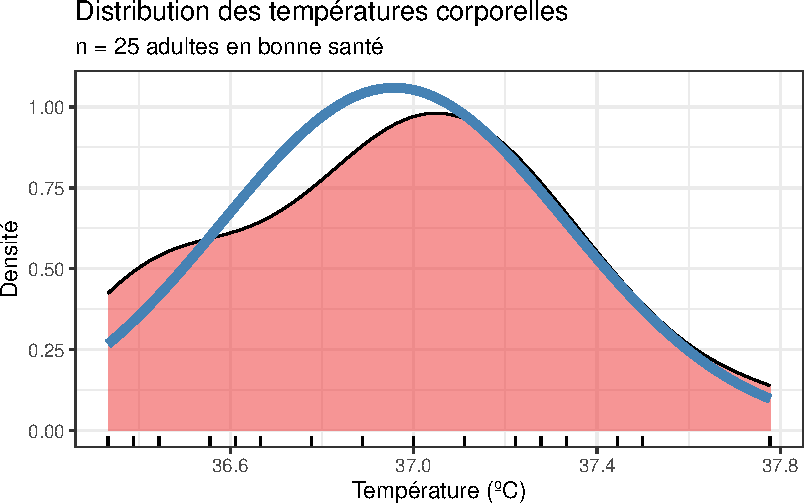
\includegraphics[keepaspectratio]{01-OneSampleTests_files/figure-pdf/unnamed-chunk-18-1.pdf}}

La courbe de densité des données observées est en rouge, et la
distribution Normale théorique correspond à la courbe en bleu. Il y a
donc un écart entre la courbe en cloche parfaite de la loi Normale et
les données observées. La \(p-\)value du test de Shapiro-Wilk nous dit
que si la température des adultes en bonne santé suit réellement la loi
Normale dans la population générale, alors, l'écart que nous avons
observé, ou un écart encore plus important, peut être observé simplement
par hasard dans 70.1\% des cas. Autrement dit, c'est très probable, et
on peut donc considérer que l'écart à la loi Normale que nous avons
observé est le fruit du hasard et que notre variable suit donc bien la
Loi Normale.

Pour bien comprendre cette notion importante, je simule ci-dessous 36
échantillons de 25 adultes dont les températures suivent parfaitement la
loi Normale dans la population générale. Je me place donc dans la
situation ou je sais que \(H_0\) est vraie, pour illustrer la notion de
\emph{fluctuation d'échantillonnage}. En raison du seul hasard de
l'échantillonnage, et alors même que les échantillons que je génère sont
issus d'une population qui suit parfaitement la Normale, la distribution
dans chaque échantillon s'écarte parfois fortement de la courbe en
cloche théorique :

\pandocbounded{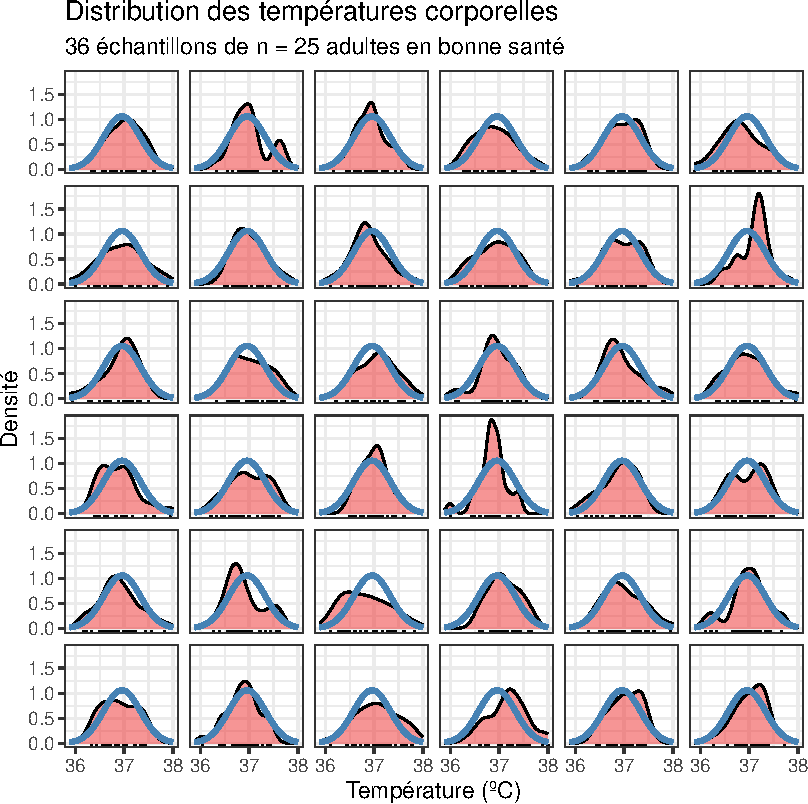
\includegraphics[keepaspectratio]{01-OneSampleTests_files/figure-pdf/unnamed-chunk-19-1.pdf}}

On voit bien ici que certains échantillons s'écartent fortement de la
distribution théorique alors même que tous les échantillons sont issus
d'une population Normale. Et plus l'échantillon sera de taille réduite,
plus les écarts à la courbe en cloche parfaite seront grands. La preuve
ci-dessous avec des échantillons de n = 15 adultes au lieu de 25 :

\pandocbounded{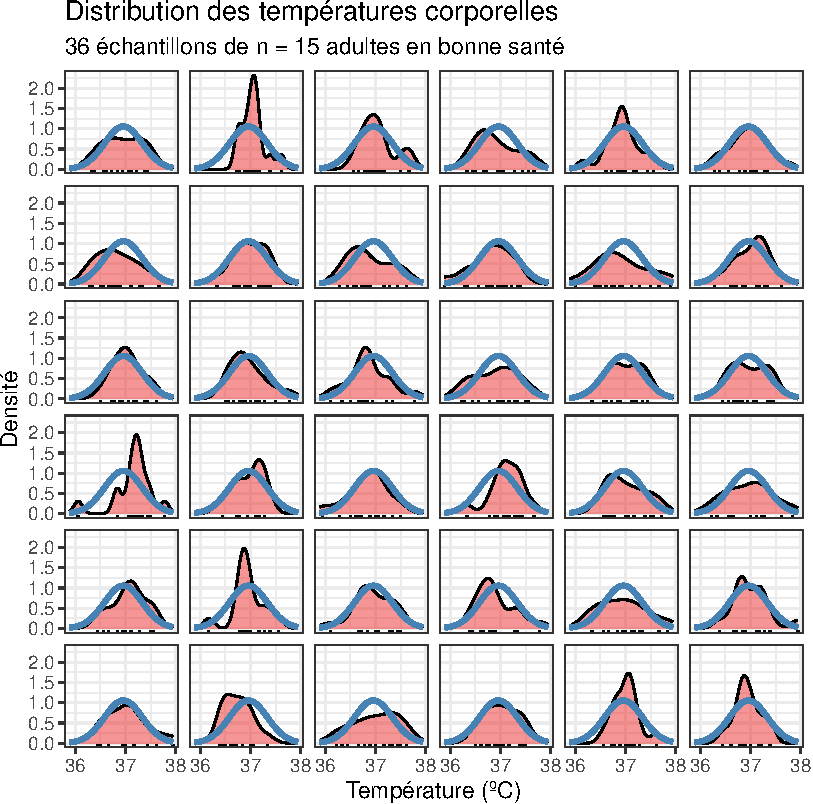
\includegraphics[keepaspectratio]{01-OneSampleTests_files/figure-pdf/unnamed-chunk-20-1.pdf}}

Au final, la \(p-\)value de 0.701 de notre test de Shapiro-Wilk nous
indique que l'hypothèse de la Normalité n'est pas incompatible avec les
données que nous avons observées.

Imaginons qu'à l'inverse, nous ayons obtenu une \(p-\)value très faible,
égale à 0.01 par exemple (donc inférieure à notre seuil \(\alpha\) de
0.05). Nous aurions alors rejeté l'hypothèse nulle. En effet, obtenir
une \(p-\)value de 0.01, signifie que si \(H_0\) est vraie, obtenir un
écart à la courbe en cloche théorique aussi important que celui que nous
observons est très peu probable (une chance sur 100). Puisqu'il est très
improbable d'observer un tel écart si \(H_0\) est vraie, on en conclu
que \(H_0\) n'est pas vraie : les données sont incompatibles avec
l'hypothèse nulle et on la rejette donc logiquement.

Cette logique sera valable pour tous les autres tests statistiques que
nous aborderons dans cet ouvrage. Pour un test de Normalité, on regarde
l'écart entre la distribution Normale et les données observées. Pour un
test de comparaison de moyennes, on regarde l'écart entre la moyenne
théorique et la moyenne observée, ou entre les 2 moyennes qu'on essaie
de comparer. Mais la philosophie reste la même.

\subsection{Réalisation du test de Student et
interprétation}\label{ruxe9alisation-du-test-de-student-et-interpruxe9tation}

Puisque les conditions d'application du test de Student à un échantillon
sont vérifiées, nous avons le droit de faire ce test, et nous devons
donc maintenant spécifier les hypothèses nulles et alternatives que nous
allons utiliser pour le réaliser :

\begin{itemize}
\tightlist
\item
  H\(_0\) : dans la population générale, la température corporelle
  moyenne des adultes en bonne santé vaut 37ºC (\(\mu = 37\)).
\item
  H\(_1\) : dans la population générale, la température corporelle
  moyenne des adultes en bonne santé est différente de 37ºC
  (\(\mu \neq 37\)).
\end{itemize}

\begin{tcolorbox}[enhanced jigsaw, arc=.35mm, bottomrule=.15mm, bottomtitle=1mm, breakable, colback=white, colbacktitle=quarto-callout-warning-color!10!white, colframe=quarto-callout-warning-color-frame, coltitle=black, left=2mm, leftrule=.75mm, opacityback=0, opacitybacktitle=0.6, rightrule=.15mm, title=\textcolor{quarto-callout-warning-color}{\faExclamationTriangle}\hspace{0.5em}{Hypothèses et paramètres}, titlerule=0mm, toprule=.15mm, toptitle=1mm]

Notez que les hypothèses des tests statistiques concernent toujours la
valeur d'un paramètre de la population générale, et non la valeur des
estimateurs calculés dans un échantillon.

\end{tcolorbox}

On réalise ensuite le test de la façon suivante :

\begin{Shaded}
\begin{Highlighting}[]
\FunctionTok{t.test}\NormalTok{(Temp\_clean}\SpecialCharTok{$}\NormalTok{temperature, }\AttributeTok{mu =} \DecValTok{37}\NormalTok{)}
\end{Highlighting}
\end{Shaded}

ou

\begin{Shaded}
\begin{Highlighting}[]
\FunctionTok{t.test}\NormalTok{(temperature }\SpecialCharTok{\textasciitilde{}} \DecValTok{1}\NormalTok{, }\AttributeTok{mu =} \DecValTok{37}\NormalTok{, }\AttributeTok{data =}\NormalTok{ Temp\_clean)}
\end{Highlighting}
\end{Shaded}

ou encore,

\begin{Shaded}
\begin{Highlighting}[]
\NormalTok{Temp\_clean }\SpecialCharTok{|\textgreater{}}
  \FunctionTok{pull}\NormalTok{(temperature) }\SpecialCharTok{|\textgreater{}}
  \FunctionTok{t.test}\NormalTok{(}\AttributeTok{mu =} \DecValTok{37}\NormalTok{)}
\end{Highlighting}
\end{Shaded}

\begin{verbatim}

    One Sample t-test

data:  pull(Temp_clean, temperature)
t = -0.56065, df = 24, p-value = 0.5802
alternative hypothesis: true mean is not equal to 37
95 percent confidence interval:
 36.80235 37.11321
sample estimates:
mean of x 
 36.95778 
\end{verbatim}

Les résultats fournis ont une forme particulière qui est utilisée par de
nombreuses fonctions de tests statistiques dans \texttt{R}. Ils méritent
donc qu'on s'y attarde un peu.\\
Sur la première ligne, \texttt{R} nous confirme que nous avons bien
réalisé un test de Student à un échantillon. La première ligne de
résultats fournit la valeur du \(t\) calculé (ici, -0.56), le nombre de
degrés de libertés (ici, \texttt{df} = 24), et la \(p-\)value (ici,
0.58, soit une valeur supérieure à \(\alpha\)). Cette première ligne
contient donc tous les résultats du test qu'il conviendrait de rappeler
dans un rapport. On devrait ainsi dire :

\begin{quote}
Au seuil \(\alpha\) de 5\%, le test de Student ne permet pas rejeter
l'hypothèse nulle \(\mu = 37\) (\(t = -0.56\), ddl = 24, \(p = 0.58\)).
Les données observées sont donc compatibles avec l'hypothèse selon
laquelle la température corporelle moyenne des adultes en bonne santé
vaut 37ºC.
\end{quote}

C'est de cette manière que vous devriez rapporter les résultats de ce
test dans un compte-rendu ou un rapport à partir de maintenant.

Dans les résultats du test, la ligne suivante
(\texttt{alternative\ hypothesis:\ ...}) \textbf{ne donne pas la
conclusion du test}. Il s'agit simplement d'un rappel concernant
l'hypothèse alternative qui a été utilisée pour réaliser le test. Ici,
l'hypothèse alternative utilisée est une hypothèse bilatérale
(\(\mu \neq 37\)). Nous verrons plus tard comment spécifier des
hypothèses alternatives uni-latérales, même si la plupart du temps,
mieux vaut s'abstenir de réaliser de tels tests (à moins bien sûr
d'avoir une bonne raison de le faire).

Les résultats fournis ensuite concernent, non plus le test statistique à
proprement parler, mais l'estimation. Ici, la moyenne de l'échantillon
est fournie. Il s'agit de la meilleure estimation possible de la moyenne
de la population : \(\bar{x} = \hat{\mu} = 36.96\). Comme pour toutes
les estimations, cette valeur est entachée d'incertitude liée à la
fluctuation d'échantillonnage. L'intervalle de confiance à 95\% de cette
estimation de moyenne est donc également fourni : \([36.80 ; 37.11]\).
Vous notez qu'il s'agit des mêmes valeurs que celles que nous avions
calculées dans la Section~\ref{sec-ic95}. Autrement dit, cet intervalle
contient les valeurs les plus vraisemblables pour la véritable valeur de
moyenne dans la population générale. Cela confirme bien que nous n'avons
pas prouvé au sens strict que la moyenne de la population vaut 37ºC.
Nous avons en réalité montré que nous ne pouvions pas exclure que la
moyenne de la population générale soit de 37ºC. Puisque cette valeur est
comprise dans l'intervalle de confiance, on ne peut donc pas l'exclure :
nos données sont compatibles avec cette hypothèse. Mais beaucoup
d'autres valeurs figurent aussi dans cet intervalle. Il est donc tout à
fait possible que la moyenne soit en réalité différente de 37ºC (par
exemple, 36.9ºC). Pour en être sûr, il faudrait probablement un
échantillon de plus grande taille afin de limiter l'incertitude,
d'augmenter la puissance statistique de notre test, et ainsi d'être en
mesure de détecter des différences subtiles.

\section{L'alternative non
paramétrique}\label{lalternative-non-paramuxe9trique}

Si jamais les conditions d'application du test de Student à un
échantillon n'étaient pas remplies, il faudrait alors réaliser son
équivalent non paramétrique : le \textbf{test de Wilcoxon des rangs
signés}. Ce test est moins puissant que son homologue paramétrique. On
ne l'effectue donc que lorsque l'on n'a pas le choix :

\begin{Shaded}
\begin{Highlighting}[]
\FunctionTok{wilcox.test}\NormalTok{(Temp\_clean}\SpecialCharTok{$}\NormalTok{temperature, }\AttributeTok{mu =} \DecValTok{37}\NormalTok{, }\AttributeTok{conf.int =} \ConstantTok{TRUE}\NormalTok{)}
\end{Highlighting}
\end{Shaded}

ou

\begin{Shaded}
\begin{Highlighting}[]
\FunctionTok{wilcox.test}\NormalTok{(temperature }\SpecialCharTok{\textasciitilde{}} \DecValTok{1}\NormalTok{, }\AttributeTok{mu =} \DecValTok{37}\NormalTok{, }\AttributeTok{conf.int =} \ConstantTok{TRUE}\NormalTok{, }\AttributeTok{data =}\NormalTok{ Temp\_clean)}
\end{Highlighting}
\end{Shaded}

ou encore

\begin{Shaded}
\begin{Highlighting}[]
\NormalTok{Temp\_clean }\SpecialCharTok{|\textgreater{}}
  \FunctionTok{pull}\NormalTok{(temperature) }\SpecialCharTok{|\textgreater{}}
  \FunctionTok{wilcox.test}\NormalTok{(}\AttributeTok{mu =} \DecValTok{37}\NormalTok{, }\AttributeTok{conf.int =} \ConstantTok{TRUE}\NormalTok{)}
\end{Highlighting}
\end{Shaded}

\begin{verbatim}
Warning in wilcox.test.default(pull(Temp_clean, temperature), mu = 37, conf.int
= TRUE): cannot compute exact p-value with ties
\end{verbatim}

\begin{verbatim}
Warning in wilcox.test.default(pull(Temp_clean, temperature), mu = 37, conf.int
= TRUE): cannot compute exact confidence interval with ties
\end{verbatim}

\begin{verbatim}

    Wilcoxon signed rank test with continuity correction

data:  pull(Temp_clean, temperature)
V = 143, p-value = 0.6077
alternative hypothesis: true location is not equal to 37
95 percent confidence interval:
 36.77780 37.11114
sample estimates:
(pseudo)median 
      36.94446 
\end{verbatim}

La syntaxe est identique à celle du test de Student à un échantillon à
une exception près : l'ajout de l'argument \texttt{conf.int\ =\ TRUE}
qui permet d'afficher la (pseudo)médiane de l'échantillon et son
intervalle de confiance à 95\%.

Les hypothèses nulles et alternatives de ce test sont les mêmes que
celles du test de Student à un échantillon. En toute rigueur, on compare
la médiane à une valeur théorique, et non la moyenne. Mais dans la
pratique, la grande majorité des utilisateurs de ce test font l'amalgame
entre moyenne et médiane. Ici, la conclusion correcte devrait donc être
:

\begin{quote}
Au seuil \(\alpha\) de 5\%, on ne peut pas rejeter l'hypothèse nulle
(test de Wilcoxon des rangs signés, \(V\) = 143, \(p\) = 0.6077). La
médiane de la population (\(\widehat{med}\) = 36.94) n'est pas
significativement différente de 37ºC (IC 95\% : \([36.78 ; 37.11]\)).
\end{quote}

Si les données ne suivent pas la loi Normale, la médiane est bien la
métrique la plus intéressante puisque c'est elle qui nous renseigne sur
la tendance centrale des données.

Enfin, les tests de Wilcoxon renvoient souvent des messages
d'avertissement. Il ne s'agit que de ça : des avertissements. Tant que
la \(p\)-value d'un test est éloignée de la valeur seuil \(\alpha\),
cela n'a pas d'importance. Quand en revanche la \(p\)-value est très
proche de \(\alpha\), les messages d'avertissement doivent vous alerter
: il faut être très prudent face aux conclusions du test qui peuvent
alors être assez ``fragiles''.

\section{Les notions d'erreur et de puissance
statistique}\label{sec-puiss}

Pour avoir le droit de réaliser un test paramétrique, il faut au
préalable vérifier qu'un certain nombre de conditions sont vérifiées. Si
ce n'est pas le cas, on réalise un équivalent non paramétrique. On peut
alors se demander pourquoi ne pas se contenter de faire des tests non
paramétrique systématiquement, sans s'embêter à faire des tests
supplémentaires ou des tests paramétriques.

La raison est simple et elle est liée aux notions d'erreur et de
puissance statistique.

\begin{tcolorbox}[enhanced jigsaw, arc=.35mm, bottomrule=.15mm, bottomtitle=1mm, breakable, colback=white, colbacktitle=quarto-callout-tip-color!10!white, colframe=quarto-callout-tip-color-frame, coltitle=black, left=2mm, leftrule=.75mm, opacityback=0, opacitybacktitle=0.6, rightrule=.15mm, title=\textcolor{quarto-callout-tip-color}{\faLightbulb}\hspace{0.5em}{Définitions}, titlerule=0mm, toprule=.15mm, toptitle=1mm]

\begin{itemize}
\item
  \textbf{Erreur de type I} : notée \(\alpha\), c'est la probabilité de
  rejeter à tort l'hypothèse nulle. C'est donc la probabilité de rejeter
  \(H_0\) alors qu'elle est vraie.
\item
  \textbf{Erreur de type II} : notée \(\beta\), c'est la probabilité
  d'accepter à tort l'hypothèse nulle. C'est donc la probabilité
  d'accepter \(H_0\) alors qu'elle est fausse.
\item
  \textbf{Puissance statistique} : notée 1 - \(\beta\)), c'est la
  probabilité de rejeter l'hypothèse nulle à raison. C'est donc la
  probabilité de rejeter \(H_0\) quand elle est réellement fausse.
\end{itemize}

\end{tcolorbox}

À chaque fois que l'on réalise un test statistique, on commet
nécessairement les 2 types d'erreurs \(\alpha\) et \(\beta\). On
souhaite évidemment minimiser les erreurs, mais on ne peut
malheureusement pas faire baisser les 2 en même temps. Faire baisser
\(\alpha\) (pour diminuer les faux positifs) conduit toujours à
augmenter \(\beta\) (les faux négatifs). Faire baisser \(\alpha\)
revient en effet à accepter plus souvent l'hypothèse nulle quand elle
est vraie. Cela conduit inévitablement accepter aussi plus souvent
l'hypothèse nulle quand elle est fausse (et donc, à augmenter les faux
négatifs).

Pour bien comprendre l'enjeu associé à ces erreurs, prenons l'exemple de
notre système judiciaire. Lorsqu'un accusé est jugé, il est présumé
innocent jusqu'à preuve du contraire. Le procès est l'équivalent d'un
test statistique, avec :

\begin{itemize}
\tightlist
\item
  \(H_0\) : l'accusé est innocent
\item
  \(H_1\) : l'accusé est coupable
\end{itemize}

Commettre une erreur de type I revient à condamner à tort l'accusé (on
rejette à tort \(H_0\)), donc on condamne un innocent. À l'inverse,
commettre une erreur de type II revient à libérer un coupable (accepter
à tort \(H_0\)). Un système de justice plus strict condamnera un plus
grand nombre d'accusés, qu'ils soient coupables ou non. Un système plus
strict fera donc augmenter l'erreur de type I et baisser l'erreur de
type II. À vous de voir ce que vous préférez : libérer plus de
coupables, ou condamner plus d'innocents ?

En statistiques, la question est tranchée puisqu'on préfère maintenir
l'erreur de type I à un niveau assez faible (à 5\% ou moins), quitte à
laisser augmenter l'erreur de type II (qui est considérée comme
acceptable jusqu'à 20\% environ). Toutefois, seule l'erreur de type I
est sous notre contrôle. En effet, c'est nous qui la choisissons lorsque
l'on fixe le seuil \(\alpha\) de nos tests statistiques.

\begin{tcolorbox}[enhanced jigsaw, arc=.35mm, bottomrule=.15mm, bottomtitle=1mm, breakable, colback=white, colbacktitle=quarto-callout-important-color!10!white, colframe=quarto-callout-important-color-frame, coltitle=black, left=2mm, leftrule=.75mm, opacityback=0, opacitybacktitle=0.6, rightrule=.15mm, title=\textcolor{quarto-callout-important-color}{\faExclamation}\hspace{0.5em}{À retenir}, titlerule=0mm, toprule=.15mm, toptitle=1mm]

C'est vous qui fixez l'erreur de type I lorsque vous faites un test
statistique. L'erreur de type I est le seuil \(\alpha\) du test, que
l'on fixe en général à 0,05 (soit 5\%) dans le domaine des sciences du
vivant.

\end{tcolorbox}

Une fois que le seuil \(\alpha\) est fixé, l'erreur \(\beta\) l'est
aussi dans une certaine mesure. Mais on ne peut la connaitre avec
précision car elle dépend de beaucoup de choses, notamment la taille des
échantillons dont on dispose, la variabilité des données, le type de
test réalisé, etc. En général, \textbf{plus la taille de l'échantillon
sera grande, plus l'erreur \(\beta\) sera faible, et donc plus la
puissance sera élevée}. De même, par rapport aux tests non
paramétriques, les tests paramétriques permettent de minimiser l'erreur
\(\beta\) et donc d'augmenter la puissance.

Puisque la puissance statistique vaut \(1 - \beta\), cela revient à dire
que les tests paramétriques sont plus puissants que les tests non
paramétriques (parfois, beaucoup plus). Au contraire des erreurs de type
I et II, la puissance est une grandeur que l'on souhaite maximiser. On
aimerait en effet être capables de systématiquement rejeter \(H_0\)
quand elle est fausse. Nous avons vu plus haut que c'est hélas
impossible. Mais choisir le bon test et la bonne procédure statistique
permettent néanmoins d'augmenter la puissance, jusqu'à un certain point.
C'est la raison pour laquelle on réalisera toujours un test paramétrique
si les données dont on dispose le permettent (donc si les conditions
d'application des tests paramétriques sont respectées). Et ce n'est
qu'en dernier recours qu'on se tournera vers les tests non
paramétriques, toujours moins puissants.

\begin{tcolorbox}[enhanced jigsaw, arc=.35mm, bottomrule=.15mm, bottomtitle=1mm, breakable, colback=white, colbacktitle=quarto-callout-important-color!10!white, colframe=quarto-callout-important-color-frame, coltitle=black, left=2mm, leftrule=.75mm, opacityback=0, opacitybacktitle=0.6, rightrule=.15mm, title=\textcolor{quarto-callout-important-color}{\faExclamation}\hspace{0.5em}{Important}, titlerule=0mm, toprule=.15mm, toptitle=1mm]

Un test paramétrique est toujours plus puissant que ses homologues non
paramétriques. Avec un test paramétrique, il est donc plus probable de
rejeter \(H_0\) à raison qu'avec un test non paramétrique.

\end{tcolorbox}

\section{Bilan}\label{bilan}

Nous avons vu dans ce chapitre quelle est la procédure à suivre pour
réaliser un test de comparaison de la moyenne d'une population à une
valeur théorique :

\begin{enumerate}
\def\labelenumi{\arabic{enumi}.}
\tightlist
\item
  examen préliminaire des données
\item
  calcul de statistiques descriptives
\item
  création de graphiques exploratoires
\item
  vérification des conditions d'application du test paramétrique
\item
  réalisation du test paramétrique ou non paramétrique selon l'issue de
  l'étape 4
\end{enumerate}

Mais nous avons aussi abordé des notions statistiques essentielles pour
la suite :

\begin{enumerate}
\def\labelenumi{\arabic{enumi}.}
\tightlist
\item
  Les ingrédients indispensables pour réaliser un test statistique (les
  hypothèses nulle et alternative, la statistique du test et le seuil
  \(\alpha\)).
\item
  La \(p-\)value et la décision du test.
\item
  Les erreurs de type I (\(\alpha\)) et II (\(\beta\)).
\item
  La puissance statistique (1 - \(\beta\)) qui n'a rien à voir avec la
  notion de précision.
\item
  La notion de test paramétrique ou non paramétrique.
\end{enumerate}

Assurez-vous d'avoir les idées claires sur toutes ces notion car elles
sont absolument centrales pour ne pas faire/dire de bêtises lorsque l'on
analyse des données.

\section{Exercice d'application}\label{sec-exo1}

\href{data/Temperature2.csv}{Le fichier \texttt{Temperature2.csv}}
contient les données brutes d'une seconde étude similaire, réalisée à
plus grande échelle. Importez ces données et analysez-les afin de
vérifier si la température corporelle moyenne des adultes en bonne santé
vaut bien 37ºC. Comme toujours, avant de vous lancer dans la réalisation
des tests statistiques, prenez le temps d'examiner vos données comme
nous l'avons décrit dans la Section~\ref{sec-eda} et la
Section~\ref{sec-edagraph}, afin de savoir où vous allez, et de repérer
les éventuelles données manquantes ou aberrantes. Enfin, interprétez les
résultats à la lumière des notions que nous avons abordées ici (en
particulier la notion de puissance statistique).

\bookmarksetup{startatroot}

\chapter{Comparaison de moyennes : deux échantillons
appariés}\label{sec-moy2}

\section{Pré-requis}\label{sec-packages2}

Pour ce nouveau chapitre, je vous conseille de travailler dans un
nouveau script que vous placerez dans votre répertoire de travail, et
dans une nouvelle session de travail (Menu
\texttt{Session\ \textgreater{}\ Restart\ R}). Inutile en revanche de
créer un nouveau \texttt{Rproject} : vous pouvez tout à fait avoir
plusieurs script dans le même répertoire de travail et pour un même
\texttt{Rproject}. Comme toujours, consultez
\href{https://besibo.github.io/BiometrieS3/01-R-basics.html\#sec-code}{le
livre en ligne du semestre 3} si vous ne savez plus comment faire.

Si vous êtes dans une nouvelle session de travail (ou que vous avez
quitté puis relancé \texttt{RStudio}), vous devrez penser à recharger en
mémoire les packages utiles. Dans ce chapitre, vous aurez besoin
d'utiliser les mêmes packages que précédemment :

\begin{itemize}
\tightlist
\item
  le \texttt{tidyverse} (Wickham 2023), qui comprend notamment le
  package \texttt{readr} (Wickham et al. 2024), pour importer facilement
  des fichiers \texttt{.csv} au format \texttt{tibble}, le package
  \texttt{dplyr} (Wickham et al. 2023), pour manipuler des tableaux, et
  le package \texttt{ggplot2} ({Wickham, Chang, et al.} 2025) pour les
  représentations graphiques.
\item
  \texttt{skimr} (Waring et al. 2022), qui permet de calculer des
  résumés de données très informatifs.
\end{itemize}

\begin{Shaded}
\begin{Highlighting}[]
\FunctionTok{library}\NormalTok{(tidyverse)}
\FunctionTok{library}\NormalTok{(skimr)}
\end{Highlighting}
\end{Shaded}

Vous aurez également besoin des jeux de données suivants que vous pouvez
dès maintenant télécharger dans votre répertoire de travail :

\begin{itemize}
\tightlist
\item
  \href{data/Autruches.csv}{\texttt{Autruches.csv}}
\item
  \href{data/Testosterone.csv}{\texttt{Testosterone.csv}}
\end{itemize}

Enfin, je spécifie ici une fois pour toutes le thème que j'utiliserai
pour tous les graphiques de ce chapitre. Libre à vous de choisir un
thème différent ou de vous contenter du thème proposé par défaut :

\begin{Shaded}
\begin{Highlighting}[]
\FunctionTok{theme\_set}\NormalTok{(}\FunctionTok{theme\_bw}\NormalTok{())}
\end{Highlighting}
\end{Shaded}

\section{Contexte}\label{contexte-1}

On s'intéresse ici à la comparaison de 2 séries de données dont les
observations sont liées 2 à 2. C'est par exemple le cas lorsque l'on
fait subir un traitement à différents sujets et que l'on souhaite
comparer les mesures obtenues avant et après le traitement.

Autrement dit, dans les plans d'expériences appariés, \textbf{les deux
traitements} ou modalités \textbf{sont appliqués à chaque unité
d'échantillonnage} : chaque sujet ou unité d'échantillonnage fournit
plusieurs valeurs. Ça n'était pas le cas du chapitre précédent
(Chapitre~\ref{sec-moy1}) où chaque adulte n'avait fourni qu'une unique
valeur de température.

Voici quelques exemples de situations qui devraient être traitées avec
des tests sur données appariées :

\begin{itemize}
\tightlist
\item
  Comparaison de la masse de patients avant et après une
  hospitalisation.
\item
  Comparaison de la diversité de peuplements de poissons dans des lacs
  avant et après contamination par des métaux lourds.
\item
  Test des effets d'une crème solaire appliquée sur un bras de chaque
  volontaire alors que l'autre bras ne reçoit qu'un placébo.
\item
  Test des effets du tabagisme dans un échantillon de fumeurs, dont
  chaque membre est comparé à un non fumeur choisi pour qu'il lui
  ressemble le plus possible en terme d'âge, de masse, d'origine
  ethnique et sociale, etc.
\item
  Test des effets que les conditions socio-économiques ont sur les
  préférences alimentaires en comparant des vrais jumeaux élevés dans
  des familles adoptives séparées qui diffèrent en termes de conditions
  socio-économiques.
\end{itemize}

Les 2 derniers exemples montrent que même des individus séparés peuvent
constituer une ``paire statistique'' s'ils partagent un certain nombre
de caractéristiques (physiques, environnementales, génétiques,
comportementales, etc.) pertinentes pour l'étude.

Ici, nous allons nous intéresser au lien qui pourrait exister entre la
production de testostérone et l'immunité chez une espèce d'oiseau vivant
en Amérique du Nord,
\href{https://fr.wikipedia.org/wiki/Carouge_à_épaulettes}{le carouge à
épaulettes}.

\begin{figure}[H]

{\centering 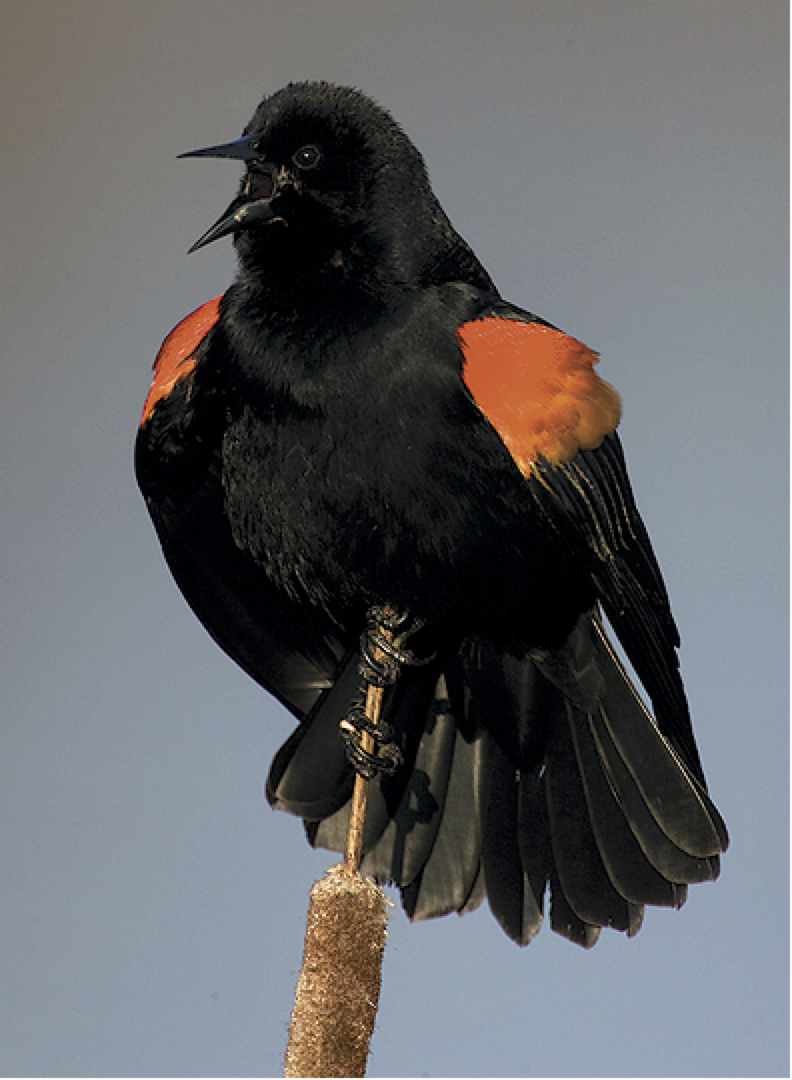
\includegraphics[width=0.5\linewidth,height=\textheight,keepaspectratio]{images/Blackbirds.png}

}

\caption{Le carouge à épaulettes}

\end{figure}%

Chez de nombreuses espèces, les mâles ont plus de chances d'attirer des
femelles s'ils produisent des niveaux de testostérone élevés. Est-ce que
la forte production de testostérone de certains mâles a un coût,
notamment en terme d'immunocompétence ? Autrement dit, est-ce que
produire beaucoup de testostérone au moment de la reproduction (ce qui
fournit un avantage sélectif) se traduit par une immunité plus faible
par la suite, et donc une plus forte susceptibilité de contracter des
maladies (ce qui constitue donc un désavantage sélectif) ? Ce type de
question est central pour comprendre comment l'allocation des ressources
affecte à la fois la survie et la fécondité des individus.

Pour étudier cette question, une équipe de chercheurs (Hasselquist et
al. 1999) a mis en place le dispositif expérimental suivant. Les niveaux
de testostérone de 13 carouges à épaulettes mâles ont été
artificiellement augmentés par l'implantation chirurgicale d'un
microtube perméable contenant de la testostérone. L'immunocompétence a
été mesurée pour chaque oiseau avant et après l'opération chirurgicale.
La variable mesurée est la production d'anticorps suite à l'exposition
des oiseaux avec un antigène non pathogène mais censé déclencher une
réponse immunitaire. Les taux de production d'anticorps sont exprimés en
logarithmes de densité optique par minute
\(\left(\ln\frac{mOD}{min}\right)\). Si la production de testostérone
influence l'immunocompétence, on s'attend à observer des différence de
production d'anticorps avant et après l'intervention chirurgicale.

\section{Importation et mise en forme des
données}\label{importation-et-mise-en-forme-des-donnuxe9es-1}

Les données se trouvent dans le fichier
\href{data/Testosterone.csv}{\texttt{Testosterone.csv}}. Importez ces
données dans un objet nommé \texttt{Testo} et affichez son contenu.

\begin{Shaded}
\begin{Highlighting}[]
\NormalTok{Testo}
\end{Highlighting}
\end{Shaded}

\begin{verbatim}
# A tibble: 13 x 5
   blackbird beforeImplant afterImplant logBeforeImplant logAfterImplant
       <dbl>         <dbl>        <dbl>            <dbl>           <dbl>
 1         1           105           85             4.65            4.44
 2         2            50           74             3.91            4.3 
 3         3           136          145             4.91            4.98
 4         4            90           86             4.5             4.45
 5         5           122          148             4.8             5   
 6         6           132          148             4.88            5   
 7         7           131          150             4.88            5.01
 8         8           119          142             4.78            4.96
 9         9           145          151             4.98            5.02
10        10           130          113             4.87            4.73
11        11           116          118             4.75            4.77
12        12           110           99             4.7             4.6 
13        13           138          150             4.93            5.01
\end{verbatim}

Visiblement, il n'y a pas de données manquantes mais certaines variables
sont inutiles. En effet, nous aurons besoin des variables transformées
en logarithmes, mais pas des 2 colonnes \texttt{beforeImplant} et
\texttt{afterImplant}. Nous allons donc les retirer avec la fonction
\texttt{select()}. Par ailleurs, la variable \texttt{blackbird} est
importante puisque chaque individu a fourni 2 valeurs de production
d'anticorps : 1 avant et 1 après l'opération chirurgicale. Il sera donc
important de conserver cet identifiant individuel. Toutefois, il
apparaît ici sous la forme d'une variable numérique alors qu'il s'agit
d'un identifiant, d'un code. Il faut donc le transformer en facteur car
cela n'aurait pas de sens calculer une moyenne des identifiants par
exemple. Pour cela, nous utiliserons la fonction \texttt{factor()} à
l'intérieur de \texttt{mutate()}. Enfin, nous renommerons les colonnes
avec \texttt{rename()} pour avoir des noms plus courts et plus faciles à
utiliser. Si vous ne vous rappelez plus comment utilisez ces fonctions,
consulter ces chapitres du livre en ligne de biométrie du semestre 3 :
\href{https://besibo.github.io/BiometrieS3/04-DataWrangling.html\#sélectionner-des-variables-avec-select}{\texttt{select()}
et \texttt{rename()}},
\href{https://besibo.github.io/BiometrieS3/04-DataWrangling.html\#mutate}{\texttt{mutate()}
et \texttt{factor()}}. Enfin, nous donnerons le nom
\texttt{Testo\_large} au tableau modifié :

\begin{Shaded}
\begin{Highlighting}[]
\NormalTok{Testo\_large }\OtherTok{\textless{}{-}}\NormalTok{ Testo }\SpecialCharTok{|\textgreater{}} 
  \FunctionTok{select}\NormalTok{(}\SpecialCharTok{{-}}\NormalTok{beforeImplant, }\SpecialCharTok{{-}}\NormalTok{afterImplant) }\SpecialCharTok{|\textgreater{}}  \CommentTok{\# Suppression des colonnes inutiles}
  \FunctionTok{mutate}\NormalTok{(}\AttributeTok{blackbird =} \FunctionTok{factor}\NormalTok{(blackbird)) }\SpecialCharTok{|\textgreater{}}  \CommentTok{\# Transformation en facteur }
  \FunctionTok{rename}\NormalTok{(}\AttributeTok{ID =}\NormalTok{ blackbird,                     }\CommentTok{\# Changement des noms de variables}
         \AttributeTok{Before =}\NormalTok{ logBeforeImplant,}
         \AttributeTok{After =}\NormalTok{ logAfterImplant)}

\NormalTok{Testo\_large}
\end{Highlighting}
\end{Shaded}

\begin{verbatim}
# A tibble: 13 x 3
   ID    Before After
   <fct>  <dbl> <dbl>
 1 1       4.65  4.44
 2 2       3.91  4.3 
 3 3       4.91  4.98
 4 4       4.5   4.45
 5 5       4.8   5   
 6 6       4.88  5   
 7 7       4.88  5.01
 8 8       4.78  4.96
 9 9       4.98  5.02
10 10      4.87  4.73
11 11      4.75  4.77
12 12      4.7   4.6 
13 13      4.93  5.01
\end{verbatim}

Le tableau \texttt{Testo\_large} dont nous disposons maintenant n'est
pas dans un format qui nous permettra de réaliser toutes les opérations
dont nous aurons besoin. En réalité, il ne s'agit pas d'un ``tableau
rangé'' au sens du tidyverse. Un tableau rangé est un tableau dans
lequel chaque ligne correspond à une unique observation et chaque
colonne correspond à une unique variable. Ici, nous devrions avoir les 3
variables suivantes :

\begin{enumerate}
\def\labelenumi{\arabic{enumi}.}
\tightlist
\item
  L'identifiant des individus. La colonne \texttt{ID} correspond à cette
  variable.
\item
  Le moment auquel chaque mesure a été effectuée, avant ou après
  l'opération chirurgicale. Cette information est pour l'instant stockée
  dans l'en-tête des colonnes 2 et 3 du tableau \texttt{Testo\_large}
\item
  La mesure de réponse immunitaire (en logarithme de la densité optique
  par minute). Cette information est pour l'instant stockée sous forme
  de valeurs numériques dans les colonnes 2 et 3 du tableau
  \texttt{Testo\_large}
\end{enumerate}

Pour obtenir un tableau rangé, il nous faut donc réorganiser les
colonnes 2 et 3 du tableau \texttt{Testo\_large} :

\begin{itemize}
\tightlist
\item
  l'entête de ces 2 colonnes devrait constituer une nouvelle variable
  que nous nommerons \texttt{Moment}
\item
  le contenu de ces 2 colonnes (les valeurs numériques) devrait
  constituer une nouvelle variable que nous nommerons \texttt{DO} (pour
  densité optique).
\end{itemize}

Pour effectuer cette transformation, nous utiliserons la fonction
\texttt{pivot\_longer()} du package \texttt{tidyr} (il est déjà chargé
en mémoire si vous avez chargé le \texttt{tidyverse}). Comme son nom
l'indique, cette fonction produira un tableau plus ``long'' (qui aura
plus de lignes) que le tableau de départ. Nous l'appellerons donc
\texttt{Testo\_long} :

\begin{Shaded}
\begin{Highlighting}[]
\NormalTok{Testo\_long }\OtherTok{\textless{}{-}}\NormalTok{ Testo\_large }\SpecialCharTok{|\textgreater{}}
  \FunctionTok{pivot\_longer}\NormalTok{(}\AttributeTok{cols =} \FunctionTok{c}\NormalTok{(Before, After),   }\CommentTok{\# Les colonnes qu\textquotesingle{}on veut réorganiser}
               \AttributeTok{names\_to =} \StringTok{"Moment"}\NormalTok{,   }\CommentTok{\# Quel nom donner à la variable qui contiendra les noms des anciennes colonnes}
               \AttributeTok{values\_to =} \StringTok{"DO"}\NormalTok{) }\SpecialCharTok{|\textgreater{}}      \CommentTok{\# Quel nom donner à la variable qui contiendra le contenu des anciennes colonnes}
  \FunctionTok{mutate}\NormalTok{(}\AttributeTok{Moment =} \FunctionTok{factor}\NormalTok{(Moment, }\AttributeTok{levels =} \FunctionTok{c}\NormalTok{(}\StringTok{"Before"}\NormalTok{, }\StringTok{"After"}\NormalTok{)))}

\NormalTok{Testo\_long}
\end{Highlighting}
\end{Shaded}

\begin{verbatim}
# A tibble: 26 x 3
   ID    Moment    DO
   <fct> <fct>  <dbl>
 1 1     Before  4.65
 2 1     After   4.44
 3 2     Before  3.91
 4 2     After   4.3 
 5 3     Before  4.91
 6 3     After   4.98
 7 4     Before  4.5 
 8 4     After   4.45
 9 5     Before  4.8 
10 5     After   5   
# i 16 more rows
\end{verbatim}

Ce nouvel objet contient les mêmes données que précédemment, mais sous
un format différent (il contient maintenant 26 lignes et non plus 13) :
il s'agit d'un tableau rangé.

La plupart du temps, on a besoin de ces 2 formats de tableaux quand nous
traitons des données. Le tableau au format long est à privilégier pour
les représentations graphiques et les tests statistiques, et le format
court sert souvent à présenter des résultats sous une forme synthétique.
Mais parfois (et c'est justement le cas quand on dispose de données
appariées comme pour notre exemple de lien entre testostérone et
immunocompétence), le tableau au format large permettra de faire
certains graphiques, certains tests ou certaines manipulations plus
facilement que le tableau rangé au format long.\\
Si on ne dispose que d'un tableau au format large, on peut passer au
format long, comme nous venons de le faire, grâce à la fonction
\texttt{pivot\_longer()}. Et si on ne dispose que d'un tableau au format
long, on peut passer au format large grâce à la fonction
\texttt{pivot\_wider()}. Nous avons déjà évoqué cette fonction dans le
livre en ligne de biométrie du semestre 4 pour mettre en forme des
résultats obtenus avec \texttt{summarise()}
(\href{https://besibo.github.io/BiometrieS4/01-dispersion.html\#grouper-par-plus-dune-variable}{par
exemple ici}) ou \texttt{reframe()}
(\href{https://besibo.github.io/BiometrieS4/01-dispersion.html\#créer-des-résumés-avec-la-fonction-reframe}{ou
là}), et je vous encourage à y jeter un œil à nouveau pour vous
remémorer la syntaxe. Car il est important que vous maîtrisiez ces 2
fonctions dont vous aurez très souvent besoin.

Maintenant que nous disposons de ces 2 tableaux, \texttt{Testo\_large}
et \texttt{Testo\_long}, nous pouvons commencer à décrire nos données.

\section{Exploration statistique des
données}\label{exploration-statistique-des-donnuxe9es}

Pour décrire simplement les données, nous nous en tiendront ici à
l'utilisation des fonctions \texttt{summary()} et \texttt{skim()}.

Pour la fonction \texttt{summary()}, le plus simple est toujours
d'utiliser le tableau au format large :

\begin{Shaded}
\begin{Highlighting}[]
\FunctionTok{summary}\NormalTok{(Testo\_large)}
\end{Highlighting}
\end{Shaded}

\begin{verbatim}
       ID        Before          After     
 1      :1   Min.   :3.910   Min.   :4.30  
 2      :1   1st Qu.:4.700   1st Qu.:4.60  
 3      :1   Median :4.800   Median :4.96  
 4      :1   Mean   :4.734   Mean   :4.79  
 5      :1   3rd Qu.:4.880   3rd Qu.:5.00  
 6      :1   Max.   :4.980   Max.   :5.02  
 (Other):7                                 
\end{verbatim}

On constate ici que pour les 2 traitements, les valeurs des différents
indices sont très proches entre les 2 séries de données, avec des
valeurs de densité optiques (DO) légèrement supérieures après
l'opération chirurgicale (sauf pour le premier quartile).

Pour la fonction \texttt{skim()} le plus simple est là aussi d'utiliser
le tableau large :

\begin{Shaded}
\begin{Highlighting}[]
\FunctionTok{skim}\NormalTok{(Testo\_large)}
\end{Highlighting}
\end{Shaded}

\begin{verbatim}
-- Data Summary ------------------------
                           Values     
Name                       Testo_large
Number of rows             13         
Number of columns          3          
_______________________               
Column type frequency:                
  factor                   1          
  numeric                  2          
________________________              
Group variables            None       

-- Variable type: factor -------------------------------------------------------
  skim_variable n_missing complete_rate ordered n_unique top_counts            
1 ID                    0             1 FALSE         13 1: 1, 2: 1, 3: 1, 4: 1

-- Variable type: numeric ------------------------------------------------------
  skim_variable n_missing complete_rate mean    sd   p0 p25  p50  p75 p100 hist 
1 Before                0             1 4.73 0.280 3.91 4.7 4.8  4.88 4.98 ▁▁▁▃▇
2 After                 0             1 4.79 0.262 4.3  4.6 4.96 5    5.02 ▂▁▂▁▇
\end{verbatim}

On arrive toutefois aux mêmes résultats avec le tableau long, à
condition de grouper les données par traitement (variable
\texttt{Traitement}) avec \texttt{group\_by()} :

\begin{Shaded}
\begin{Highlighting}[]
\NormalTok{Testo\_long }\SpecialCharTok{|\textgreater{}}
  \FunctionTok{group\_by}\NormalTok{(Moment) }\SpecialCharTok{|\textgreater{}}
  \FunctionTok{skim}\NormalTok{(DO)}
\end{Highlighting}
\end{Shaded}

\begin{verbatim}
-- Data Summary ------------------------
                           Values                      
Name                       group_by(Testo_long, Mome...
Number of rows             26                          
Number of columns          3                           
_______________________                                
Column type frequency:                                 
  numeric                  1                           
________________________                               
Group variables            Moment                      

-- Variable type: numeric ------------------------------------------------------
  skim_variable Moment n_missing complete_rate mean    sd   p0 p25  p50  p75
1 DO            Before         0             1 4.73 0.280 3.91 4.7 4.8  4.88
2 DO            After          0             1 4.79 0.262 4.3  4.6 4.96 5   
  p100 hist 
1 4.98 ▁▁▁▃▇
2 5.02 ▂▁▂▁▇
\end{verbatim}

Cela revient à demander à la fonction \texttt{skim()} de produire un
résumé des données de densité optique (variable \texttt{DO}), pour
chaque catégorie de la variable \texttt{Moment}, soit un résumé pour la
catégorie \texttt{Before} (avant l'intervention chirurgicale), et un
résumé pour la catégorie \texttt{After} (après l'intervention
chirurgicale).

Par rapport aux résultats fournis par la fonction \texttt{summary()}, la
fonction \texttt{skim()} nous permet de confirmer que les valeurs de DO
sont très légèrement supérieures après l'opération (sauf pour le premier
quartile). Elle nous permet également de constater que l'écart-type est
du même ordre de grandeur pour les 2 catégories, bien qu'il soit
légèrement plus faible après l'opération. Enfin, les petits histogrammes
laissent entrevoir une distribution très asymétrique des données dans
chacun des 2 groupes de mesures.

\section{Exploration graphique des
données}\label{exploration-graphique-des-donnuxe9es}

Ici, c'est le tableau rangé au format long qui sera le plus adapté.
Lorsque nous avions une unique série de données, nous avons utilisé 2
types de représentations graphiques très similaires pour visualiser les
données (les histogrammes et les graphiques de densités). Ici, nous
allons utiliser ces mêmes types de graphiques mais ``facettés''. Les
graphiques facettés ont été abordés dans
\href{https://besibo.github.io/BiometrieS3/03-visualization.html\#diagrammes-bâtons-facettés}{le
livre en ligne de biométrie du semestre 3}. Ils permettent de faire des
sous-graphiques pour chaque catégorie d'un facteur. Ici, le facteur
\texttt{Moment} contient 2 catégories. Les facets nous permettrons donc
de comparer les 2 distributions de densités optiques.

Outre ces graphiques, nous utiliserons aussi les stripcharts et les
boites à moustaches pour comparer les 2 catégories. Ces 2 types de
graphiques sont particulièrement adaptés pour ce genre de tâche, et
seront aussi très utiles pour l'ANOVA lorsque nous aurons plus de 2
catégories à comparer.

D'une façon générale, nous disposons :

\begin{itemize}
\tightlist
\item
  d'une variable numérique, \texttt{DO} : la mesure de densité optique
  qui rend compte de l'immunocompétence des carouges à épaulettes
\item
  d'une variable catégorielle, le facteur \texttt{Moment} : indique si
  les valeurs d'immunocompétences ont été mesurées avant ou après
  l'opération chirurgicale d'implantation de la capsule de testostérone.
\end{itemize}

Tous les graphiques présentés dans
\href{https://besibo.github.io/BiometrieS3/03-visualization.html\#une-variable-de-chaque-type}{le
chapitre consacré à cette situation précise} dans le livre en ligne de
biométrie du semestre 3, peuvent être réalisés. N'hésitez pas à le
relire, en particulier la section expliquant comment faire apparaître et
interpréter les encoches d'incertitudes sur des boiites à moustaches.

\subsection{Avec un stripchart}\label{avec-un-stripchart}

\begin{Shaded}
\begin{Highlighting}[]
\NormalTok{Testo\_long }\SpecialCharTok{|\textgreater{}}
  \FunctionTok{ggplot}\NormalTok{(}\FunctionTok{aes}\NormalTok{(}\AttributeTok{x =}\NormalTok{ Moment, }\AttributeTok{y =}\NormalTok{ DO)) }\SpecialCharTok{+}
  \FunctionTok{geom\_jitter}\NormalTok{(}\AttributeTok{height =} \DecValTok{0}\NormalTok{, }\AttributeTok{width =} \FloatTok{0.25}\NormalTok{) }\SpecialCharTok{+}
  \FunctionTok{labs}\NormalTok{(}\AttributeTok{y =} \StringTok{"immunocompétence (log DO / minute)"}\NormalTok{,}
       \AttributeTok{title =} \StringTok{"immunocompétence}\SpecialCharTok{\textbackslash{}n}\StringTok{avant et après l\textquotesingle{}opération"}\NormalTok{,}
       \AttributeTok{subtitle =} \StringTok{"n = 13 carouges à épaulettes"}\NormalTok{)}
\end{Highlighting}
\end{Shaded}

\begin{center}

\includegraphics[width=0.5\linewidth,height=\textheight,keepaspectratio]{02-TwoSamplePairedTests_files/figure-pdf/unnamed-chunk-10-1.pdf}
\end{center}

\subsection{Avec des histogrammes
facettés}\label{avec-des-histogrammes-facettuxe9s}

Nous allons faire un histogramme pour chaque série de données en
utilisant des facettes :

\begin{Shaded}
\begin{Highlighting}[]
\NormalTok{Testo\_long }\SpecialCharTok{|\textgreater{}}
  \FunctionTok{ggplot}\NormalTok{(}\FunctionTok{aes}\NormalTok{(}\AttributeTok{x =}\NormalTok{ DO)) }\SpecialCharTok{+}
  \FunctionTok{geom\_histogram}\NormalTok{(}\AttributeTok{bins =} \DecValTok{10}\NormalTok{, }\AttributeTok{fill =} \StringTok{"firebrick2"}\NormalTok{, }\AttributeTok{color =} \StringTok{"grey20"}\NormalTok{, }\AttributeTok{alpha =} \FloatTok{0.5}\NormalTok{)}\SpecialCharTok{+}
  \FunctionTok{geom\_rug}\NormalTok{() }\SpecialCharTok{+}
  \FunctionTok{facet\_wrap}\NormalTok{(}\SpecialCharTok{\textasciitilde{}}\NormalTok{Moment, }\AttributeTok{ncol =} \DecValTok{1}\NormalTok{) }\SpecialCharTok{+}
  \FunctionTok{labs}\NormalTok{(}\AttributeTok{x =} \StringTok{"immunocompétence (log DO / minute)"}\NormalTok{,}
       \AttributeTok{y =} \StringTok{"Fréquence"}\NormalTok{,}
       \AttributeTok{title =} \StringTok{"Comparaison de l\textquotesingle{}immunocompétence avant et après l\textquotesingle{}opération chirurgicale"}\NormalTok{,}
       \AttributeTok{subtitle =} \StringTok{"n = 13 carouges à épaulettes"}\NormalTok{)}
\end{Highlighting}
\end{Shaded}

\pandocbounded{
\includegraphics[keepaspectratio]{02-TwoSamplePairedTests_files/figure-pdf/unnamed-chunk-11-1.pdf}}

\subsection{Avec des diagrammes de densité
facettés}\label{avec-des-diagrammes-de-densituxe9-facettuxe9s}

\begin{Shaded}
\begin{Highlighting}[]
\NormalTok{Testo\_long }\SpecialCharTok{|\textgreater{}}
  \FunctionTok{ggplot}\NormalTok{(}\FunctionTok{aes}\NormalTok{(}\AttributeTok{x =}\NormalTok{ DO)) }\SpecialCharTok{+}
  \FunctionTok{geom\_density}\NormalTok{(}\AttributeTok{fill =} \StringTok{"firebrick2"}\NormalTok{, }\AttributeTok{alpha =} \FloatTok{0.5}\NormalTok{) }\SpecialCharTok{+}
  \FunctionTok{geom\_rug}\NormalTok{() }\SpecialCharTok{+}
  \FunctionTok{facet\_wrap}\NormalTok{(}\SpecialCharTok{\textasciitilde{}}\NormalTok{Moment, }\AttributeTok{ncol =} \DecValTok{1}\NormalTok{) }\SpecialCharTok{+}
  \FunctionTok{labs}\NormalTok{(}\AttributeTok{x =} \StringTok{"immunocompétence (log DO / minute)"}\NormalTok{,}
       \AttributeTok{y =} \StringTok{"Densité"}\NormalTok{,}
       \AttributeTok{title =} \StringTok{"Comparaison de l\textquotesingle{}immunocompétence avant et après l\textquotesingle{}opération chirurgicale"}\NormalTok{,}
       \AttributeTok{subtitle =} \StringTok{"n = 13 carouges à épaulettes"}\NormalTok{)}
\end{Highlighting}
\end{Shaded}

\pandocbounded{
\includegraphics[keepaspectratio]{02-TwoSamplePairedTests_files/figure-pdf/unnamed-chunk-12-1.pdf}}

\subsection{Avec des boîtes à
moustaches}\label{avec-des-bouxeetes-uxe0-moustaches}

\begin{Shaded}
\begin{Highlighting}[]
\NormalTok{Testo\_long }\SpecialCharTok{|\textgreater{}}
  \FunctionTok{ggplot}\NormalTok{(}\FunctionTok{aes}\NormalTok{(}\AttributeTok{x =}\NormalTok{ Moment, }\AttributeTok{y =}\NormalTok{ DO)) }\SpecialCharTok{+}
  \FunctionTok{geom\_boxplot}\NormalTok{(}\AttributeTok{notch =} \ConstantTok{TRUE}\NormalTok{) }\SpecialCharTok{+}
  \FunctionTok{expand\_limits}\NormalTok{(}\AttributeTok{y =} \FloatTok{5.2}\NormalTok{) }\SpecialCharTok{+}
  \FunctionTok{labs}\NormalTok{(}\AttributeTok{y =} \StringTok{"immunocompétence (log DO / minute)"}\NormalTok{,}
       \AttributeTok{title =} \StringTok{"Comparaison de l\textquotesingle{}immunocompétence avant et après opération chirurgicale"}\NormalTok{,}
       \AttributeTok{subtitle =} \StringTok{"n = 13 carouges à épaulettes"}\NormalTok{)}
\end{Highlighting}
\end{Shaded}

\begin{verbatim}
Notch went outside hinges
i Do you want `notch = FALSE`?
\end{verbatim}

\begin{center}

\includegraphics[width=0.5\linewidth,height=\textheight,keepaspectratio]{02-TwoSamplePairedTests_files/figure-pdf/unnamed-chunk-13-1.pdf}
\end{center}

Du point de vue de la \textbf{position} des données, ces différents
graphiques montrent tous que la seconde série de données (catégorie
\texttt{After} : après l'opération chirurgicale) présente en moyenne des
valeurs très légèrement plus élevées que la première (catégorie
\texttt{Before} avant l'opération). En terme de \textbf{dispersion}, si
l'on met de côté la valeur minimale de la série \texttt{Before} qui
semble atypique (un individu outlier qui présente une immunocompétence
très faible avant l'opération), la dispersion des données autour de la
tendance centrale semble globalement plus importante pour la série
\texttt{After}. Enfin, pour ce qui concerne l'\textbf{incertitude}, les
intervalles de confiance à 95\% des médianes (qui apparaissent sous la
forme d'encoches sur les boîtes à moustaches) se chevauche assez
largement, ce qui nous permet d'anticiper les résultats des tests que
nous ferons ensuite : puisque les encoches se chevauchent, il y a fort à
parier que le test de comparaison de moyenne ne montrera aucune
différence significative. On note également que l'encoche de la série
\texttt{After} est particulièrement large : la limite supérieure de
l'intervalle de confiance à 95\% de la médiane est supérieure à la
valeur maximale observée dans l'échantillon. Cela traduit le fait que
compte de la grande variabilité des données dans cette série, un
échantillon de taille n = 13 n'est probablement pas suffisant pour avoir
une estimation précise de la médiane.

\subsection{Avec un nuage de points
appariés}\label{avec-un-nuage-de-points-appariuxe9s}

Toutes ces représentations graphiques sont certes utiles, mais elles
masquent un élément crucial : ce sont les mêmes individus qui sont
étudiés avant et après l'opération. Il s'agit de données appariées ! Les
graphiques que nous avons faits jusque là ne permettent pas de
visualiser ce lien entre les deux séries de données. Pour avoir une
bonne vision de ce qui se passe, il nous faut faire apparaître ce lien
entre les 2 séries de données :

\begin{Shaded}
\begin{Highlighting}[]
\NormalTok{Testo\_long }\SpecialCharTok{|\textgreater{}}
  \FunctionTok{ggplot}\NormalTok{(}\FunctionTok{aes}\NormalTok{(}\AttributeTok{x =}\NormalTok{ Moment, }\AttributeTok{y =}\NormalTok{ DO, }\AttributeTok{group =}\NormalTok{ ID, }\AttributeTok{color =}\NormalTok{ ID)) }\SpecialCharTok{+}
  \FunctionTok{geom\_line}\NormalTok{() }\SpecialCharTok{+}
  \FunctionTok{geom\_point}\NormalTok{() }\SpecialCharTok{+}
  \FunctionTok{labs}\NormalTok{(}\AttributeTok{y =} \StringTok{"immunocompétence (log DO / minute)"}\NormalTok{,}
       \AttributeTok{title =} \StringTok{"Comparaison de l\textquotesingle{}immunocompétence avant et après opération chirurgicale"}\NormalTok{,}
       \AttributeTok{subtitle =} \StringTok{"n = 13 carouges à épaulettes"}\NormalTok{, }
       \AttributeTok{color =} \StringTok{"Individu"}\NormalTok{)}
\end{Highlighting}
\end{Shaded}

\begin{center}

\includegraphics[width=0.5\linewidth,height=\textheight,keepaspectratio]{02-TwoSamplePairedTests_files/figure-pdf/unnamed-chunk-14-1.pdf}
\end{center}

Ce graphique nous donne une image très différente de la réalité des
données. On constate ici que l'immunocompétence de certains individus
augmente après l'opération (parfois fortement), alors que pour d'autres,
elle diminue.

Une façon d'estimer si les changements d'immunocompétence sont
majoritairement orientés dans un sens ou non est de calculer
l'intervalle de confiance à 95\% de la différence d'immunocompétence
entre avant et après l'opération. Pour cela, on peut calculer, grâce au
tableau large \texttt{Testo\_large}, les différences d'immunocompétences
(DO après opération moins DO avant opération), pour chacun des 13
individus. puis, grâce à la fonction \texttt{mean\_cl\_normal()} déjà
utilisée à plusieurs reprises, on calcul l'intervalle de confiance à
95\% de la moyenne de cette différence :

\begin{Shaded}
\begin{Highlighting}[]
\CommentTok{\# Calcul de la différence de DO (After {-} Before)}
\NormalTok{Testo\_large }\OtherTok{\textless{}{-}}\NormalTok{ Testo\_large }\SpecialCharTok{|\textgreater{}} 
  \FunctionTok{mutate}\NormalTok{(}\AttributeTok{Difference =}\NormalTok{ After }\SpecialCharTok{{-}}\NormalTok{ Before)}

\CommentTok{\# Affichage du tableau}
\NormalTok{Testo\_large}
\end{Highlighting}
\end{Shaded}

\begin{verbatim}
# A tibble: 13 x 4
   ID    Before After Difference
   <fct>  <dbl> <dbl>      <dbl>
 1 1       4.65  4.44    -0.21  
 2 2       3.91  4.3      0.390 
 3 3       4.91  4.98     0.0700
 4 4       4.5   4.45    -0.0500
 5 5       4.8   5        0.200 
 6 6       4.88  5        0.120 
 7 7       4.88  5.01     0.130 
 8 8       4.78  4.96     0.180 
 9 9       4.98  5.02     0.0400
10 10      4.87  4.73    -0.140 
11 11      4.75  4.77     0.0200
12 12      4.7   4.6     -0.100 
13 13      4.93  5.01     0.0800
\end{verbatim}

\begin{Shaded}
\begin{Highlighting}[]
\CommentTok{\# Calcul de la moyenne des différences et de son IC95\%}
\NormalTok{Testo\_large }\SpecialCharTok{|\textgreater{}} 
  \FunctionTok{reframe}\NormalTok{(}\FunctionTok{mean\_cl\_normal}\NormalTok{(Difference))}
\end{Highlighting}
\end{Shaded}

\begin{verbatim}
# A tibble: 1 x 3
       y    ymin  ymax
   <dbl>   <dbl> <dbl>
1 0.0562 -0.0401 0.152
\end{verbatim}

On constate ici que la moyenne des différences de densité optique vaut
0.06, soit une valeur positive, qui montre que l'immunocompétence
augmente après l'opération (ce qui semble aller à l'opposé de
l'hypothèse des chercheurs). Cette moyenne reste néanmoins très proche
de 0. D'ailleurs, l'intervalle de confiance de cette moyenne comprend
les valeurs situées entre -0.04 et +0.15. La valeur 0 est donc comprise
dans cet intervalle. Le zéro fait donc partie des valeurs les plus
probables pour la moyenne de ces différences dans la populations
générale. C'est là encore un résultat qui nous permet d'anticiper sur
les résultats du tests statistique que nous ferons ensuite.

\section{Le test paramétrique}\label{le-test-paramuxe9trique-1}

\subsection{Procédure}\label{procuxe9dure}

Le test paramétrique permettant de comparer la moyenne sur des séries
appariées est là encore un test de Student : le \textbf{test de Student
sur données appariées} (étonnant non ?\ldots). En réalité, ce test de
Student n'est pas un test de comparaison de moyennes entre 2 séries de
données. La procédure est la suivante :

\begin{enumerate}
\def\labelenumi{\arabic{enumi}.}
\tightlist
\item
  Pour chaque individu, calculer la différence d'immunocompétence entre
  les deux temps de l'expérience (DO après - DO avant opération). C'est
  ce que nous avons fait plus haut en ajoutant la colonne
  \texttt{Difference} au tableau \texttt{Testo\_large}.
\item
  Puisque nous avons 13 individus, nous aurons 13 valeurs de
  différences. La moyenne de cette différence sera comparée à la valeur
  théorique 0. Autrement dit, si cette moyenne vaut 0,
  l'immunocompétence sera la même avant et après l'opération. Si la
  moyenne des différence n'est pas égale 0, alors nous aurons prouvé
  qu'il existe une différence d'immunocompétence entre les 2 groupes,
  nous aurons prouvé que la procédure chirurgicale d'implantation de la
  capsule de testostérone a un impact sur l'immunocompétence des
  carouges à épaulettes
\end{enumerate}

\begin{tcolorbox}[enhanced jigsaw, arc=.35mm, bottomrule=.15mm, bottomtitle=1mm, breakable, colback=white, colbacktitle=quarto-callout-warning-color!10!white, colframe=quarto-callout-warning-color-frame, coltitle=black, left=2mm, leftrule=.75mm, opacityback=0, opacitybacktitle=0.6, rightrule=.15mm, title=\textcolor{quarto-callout-warning-color}{\faExclamationTriangle}\hspace{0.5em}{Attention}, titlerule=0mm, toprule=.15mm, toptitle=1mm]

Dans un test sur données appariées, on s'intéresse à \textbf{la moyenne
des différences} entre les données des 2 séries. Cette moyenne est alors
comparée à la valeur théorique \(\mu\) = 0. Ce test est donc équivalent
au test vu dans le Chapitre~\ref{sec-moy1} sur la comparaison de la
moyenne d'une population à une valeur théorique.

Notez également que \textbf{la moyenne des différences} n'est pas
équivalente à \textbf{la différence des moyennes}. La différence des
moyennes est une grandeur qui nous sera utile dans le chapitre suivant
(Chapitre~\ref{sec-moy3}) sur la comparaison de la moyenne de deux
populations lorsque les données sont indépendantes.

\end{tcolorbox}

\subsection{Conditions d'application}\label{conditions-dapplication}

Les conditions d'application de ce test paramétrique sont presque les
mêmes que pour le test de Student à un échantillon :

\begin{enumerate}
\def\labelenumi{\arabic{enumi}.}
\tightlist
\item
  Les individus sur lesquels portent la comparaison doivent être issus
  d'un échantillonnage aléatoire. Comme toujours, en l'absence
  d'indication contraire, on considère que cette condition est vérifiée.
\item
  Les différences par paires entre les 2 modalités du traitement doivent
  suivre une distribution Normale. Attention, ce n'est donc pas les
  données brutes de chaque série qui doivent suivre une loi Normale,
  mais bien la différence ``après'' - ``avant'' calculée pour chaque
  individu. Nous avons déjà calculé ces différences plus haut :
\end{enumerate}

\begin{Shaded}
\begin{Highlighting}[]
\CommentTok{\# On s\textquotesingle{}intéresse aux 13 différences calculées sur les 13 individus}
\NormalTok{Testo\_large }
\end{Highlighting}
\end{Shaded}

\begin{verbatim}
# A tibble: 13 x 4
   ID    Before After Difference
   <fct>  <dbl> <dbl>      <dbl>
 1 1       4.65  4.44    -0.21  
 2 2       3.91  4.3      0.390 
 3 3       4.91  4.98     0.0700
 4 4       4.5   4.45    -0.0500
 5 5       4.8   5        0.200 
 6 6       4.88  5        0.120 
 7 7       4.88  5.01     0.130 
 8 8       4.78  4.96     0.180 
 9 9       4.98  5.02     0.0400
10 10      4.87  4.73    -0.140 
11 11      4.75  4.77     0.0200
12 12      4.7   4.6     -0.100 
13 13      4.93  5.01     0.0800
\end{verbatim}

Il nous faut donc tester la Normalité de la nouvelle variable
\texttt{Difference}. Commençons par en faire un graphique :

\begin{Shaded}
\begin{Highlighting}[]
\NormalTok{Testo\_large }\SpecialCharTok{|\textgreater{}}
  \FunctionTok{ggplot}\NormalTok{(}\FunctionTok{aes}\NormalTok{(}\AttributeTok{x =}\NormalTok{ Difference)) }\SpecialCharTok{+}
  \FunctionTok{geom\_density}\NormalTok{(}\AttributeTok{fill =} \StringTok{"firebrick2"}\NormalTok{, }\AttributeTok{alpha =} \FloatTok{0.5}\NormalTok{) }\SpecialCharTok{+}
  \FunctionTok{geom\_rug}\NormalTok{() }\SpecialCharTok{+}
  \FunctionTok{labs}\NormalTok{(}\AttributeTok{x =} \StringTok{"Différence d\textquotesingle{}immunocompétence \textquotesingle{}Après {-} Avant\textquotesingle{} l\textquotesingle{}opération (log DO / minute)"}\NormalTok{,}
       \AttributeTok{y =} \StringTok{"Densité"}\NormalTok{,}
       \AttributeTok{title =} \StringTok{"Distribution de la différence d\textquotesingle{}immunocompétence entre après et avant l\textquotesingle{}opération chirurgicale"}\NormalTok{,}
       \AttributeTok{subtitle =} \StringTok{"n = 13 carouges à épaulettes"}\NormalTok{)}
\end{Highlighting}
\end{Shaded}

\pandocbounded{
\includegraphics[keepaspectratio]{02-TwoSamplePairedTests_files/figure-pdf/unnamed-chunk-17-1.pdf}}

Compte tenu du faible nombre d'individus (n = 13), la forme de cette
courbe de densité n'est pas si éloignée que ça d'une courbe en cloche
(notez que ce n'était pas du tout le cas pour les données brutes de
chaque série de départ qui ont toutes les deux des distributions très
éloignées de la distribution Normale). On le vérifie avec un test de
normalité de Shapiro-Wilk :

\begin{itemize}
\tightlist
\item
  H\(_0\) : la différence d'immunocompétence des individus suit une
  distribution Normale.
\item
  H\(_1\) : la différence d'immunocompétence des individus ne suit pas
  une distribution Normale.
\end{itemize}

\begin{Shaded}
\begin{Highlighting}[]
\NormalTok{Testo\_large }\SpecialCharTok{|\textgreater{}}
  \FunctionTok{pull}\NormalTok{(Difference) }\SpecialCharTok{|\textgreater{}}
  \FunctionTok{shapiro.test}\NormalTok{()}
\end{Highlighting}
\end{Shaded}

\begin{verbatim}

    Shapiro-Wilk normality test

data:  pull(Testo_large, Difference)
W = 0.97949, p-value = 0.977
\end{verbatim}

\begin{quote}
Au seuil \(\alpha = 0.05\), on ne peut pas rejeter l'hypothèse nulle de
normalité pour la différence d'immunocompétence entre après et avant
l'intervention chirurgicale (test de Shapiro-Wilk, \(W = 0.98\),
\(p = 0.977\)).
\end{quote}

Les conditions d'application du test paramétrique sont donc réunies.

\begin{tcolorbox}[enhanced jigsaw, arc=.35mm, bottomrule=.15mm, bottomtitle=1mm, breakable, colback=white, colbacktitle=quarto-callout-warning-color!10!white, colframe=quarto-callout-warning-color-frame, coltitle=black, left=2mm, leftrule=.75mm, opacityback=0, opacitybacktitle=0.6, rightrule=.15mm, title=\textcolor{quarto-callout-warning-color}{\faExclamationTriangle}\hspace{0.5em}{Attention !}, titlerule=0mm, toprule=.15mm, toptitle=1mm]

Pour ce test, la Normalité doit bien être vérifiée sur la différence
entre les 2 groupes de valeurs, et non sur chaque groupe de valeur pris
séparément. C'est une source d'erreur fréquente. Ici, les données de
départ (DO avant et DO après) ne suivaient pas du tout une distribution
Normale. Pourtant, la différence de DO suit bel et bien la distribution
Normale, nous permettant de faire le test paramétrique.

\end{tcolorbox}

\subsection{Réalisation du test et
interprétation}\label{ruxe9alisation-du-test-et-interpruxe9tation}

Le test de Student sur données appariées peut se faire de 2 façons
distinctes. Les 2 méthodes fournissent exactement les mêmes résultats,
seule la syntaxe utilisée change. Quelle que soit la méthode utilisée,
les hypothèses nulles et alternatives sont toujours les mêmes :

\begin{itemize}
\tightlist
\item
  H\(_0\) : le changement moyen de production d'anticorps après la pose
  chirurgicale de l'implant de testostérone est nul
  (\(\mu_{Diff} = 0\)). La procédure chirurgicale n'a pas d'effet sur
  l'immunocompétence. Les variations observées ne sont que le fruit du
  hasard de l'échantillonnage.
\item
  H\(_1\) : le changement moyen de production d'anticorps après la pose
  chirurgicale de l'implant de testostérone n'est pas nul
  (\(\mu_{Diff} \neq 0\)). La procédure chirurgicale a effet
  significatif sur l'immunocompétence. Les variations observées ne sont
  pas uniquement dues à la fluctuation d'échantillonnage.
\end{itemize}

\subsubsection{Première syntaxe}\label{premiuxe8re-syntaxe}

\begin{Shaded}
\begin{Highlighting}[]
\CommentTok{\# Méthode nº2 : avec les 2 séries de données et le tableau au format large}
\FunctionTok{t.test}\NormalTok{(Testo\_large}\SpecialCharTok{$}\NormalTok{Before, Testo\_large}\SpecialCharTok{$}\NormalTok{After, }\AttributeTok{paired =} \ConstantTok{TRUE}\NormalTok{)}
\end{Highlighting}
\end{Shaded}

\begin{verbatim}

    Paired t-test

data:  Testo_large$Before and Testo_large$After
t = -1.2714, df = 12, p-value = 0.2277
alternative hypothesis: true mean difference is not equal to 0
95 percent confidence interval:
 -0.15238464  0.04007695
sample estimates:
mean difference 
    -0.05615385 
\end{verbatim}

Avec cette première syntaxe, on indique le nom des 2 colonnes du tableau
\texttt{Testo\_large} qui contiennent les 2 séries de données. Il nous
faut taper spécifiquement ``\texttt{Testo\_large\$Before}'' et
``\texttt{Testo\_large\$After}'', et non pas simplement
``\texttt{Before}'' et ``\texttt{After}'' car la fonction
\texttt{t.test} n'a aucun moyen de savoir que ``\texttt{Before}'' et
``\texttt{After}'' sont des colonnes du tableau \texttt{Testo-large}.
Nous devons donc être explicites. Il est en outre indispensable
d'indiquer ``\texttt{paired\ =\ TRUE}'' pour faire un test de Student
sur données appariées. Omettre cet argument reviendrait à faire un test
de Student sur données indépendantes, qui est moins puissant que le test
sur données appariées. Ça n'est donc pas souhaitable avec les données
dont nous disposons et ça pourrait même conduire à des conclusions
fausses.

Ici, voilà la conclusion de ce test :

\begin{quote}
Le test de Student sur données appariées ne permet pas de montrer de
changement d'immunocompétence suite à l'intégration de l'implant
chirurgical de testostérone. On ne peut pas rejeter l'hypothèse nulle au
seuil \(\alpha = 0.05\) (\(t = -1.27\), \(ddl = 12\), \(p = 0.223\)). La
moyenne des différences de densités optiques observées entre avant et
après l'intervention chirurgicale vaut -0.056 (intervalle de confiance à
95\% de cette différence : {[}-0.152 ; 0.040{]})
\end{quote}

Donc visiblement, une forte production de testostérone n'est pas
significativement associée à une baisse de l'immunocompétence.

Notez bien que les résultats et leurs interprétation dépendent de
l'ordre dans lequel les 2 séries de données sont indiquées dans la
fonction \texttt{t.test()}. Pour vous en convaincre, regardez ce que
donne cette commande :

\begin{Shaded}
\begin{Highlighting}[]
\FunctionTok{t.test}\NormalTok{(Testo\_large}\SpecialCharTok{$}\NormalTok{After, Testo\_large}\SpecialCharTok{$}\NormalTok{Before, }\AttributeTok{paired =} \ConstantTok{TRUE}\NormalTok{)}
\end{Highlighting}
\end{Shaded}

Qu'est-ce qui change ? Et qu'est-ce qui reste inchangé ?

\subsubsection{Deuxième syntaxe}\label{deuxiuxe8me-syntaxe}

\begin{Shaded}
\begin{Highlighting}[]
\CommentTok{\# Méthode nº3 : avec la variable Diff, mu = 0, et le tableau au format large}
\FunctionTok{t.test}\NormalTok{(Testo\_large}\SpecialCharTok{$}\NormalTok{Difference, }\AttributeTok{mu =} \DecValTok{0}\NormalTok{)}
\end{Highlighting}
\end{Shaded}

\begin{verbatim}

    One Sample t-test

data:  Testo_large$Difference
t = 1.2714, df = 12, p-value = 0.2277
alternative hypothesis: true mean is not equal to 0
95 percent confidence interval:
 -0.04007695  0.15238464
sample estimates:
 mean of x 
0.05615385 
\end{verbatim}

Comme expliqué plus haut, le test de Student sur données appariées est
strictement équivalent à un test de Student à un échantillon pour lequel
on compare la moyenne des différences individuelles à 0. Là encore, les
résultats produits et leur interprétation sont identiques aux deux tests
précédents. La seule différence concerne les signes puisque le premier
test regardait la différence ``Before - After'' alors que ce test
regarde la différence ``After - Before'' (que nous avons calculée
manuellement).

À vous donc de choisir la syntaxe qui vous paraît la plus parlante ou
celle que vous avez le plus de facilité à retenir et à interpréter.

\section{L'alternative non
paramétrique}\label{lalternative-non-paramuxe9trique-1}

Comme pour le test de Student à un échantillon, lorsque les conditions
d'application du test de Student sur données appariées ne sont pas
vérifiées (c'est à dire lorsque la différence entre les données
appariées des deux séries ne suit pas une loi Normale), il faut utiliser
un test non paramétrique équivalent.

Il s'agit là encore du \textbf{test de Wilcoxon des rangs signés} qui
s'intéresse aux médianes. Les hypothèses nulles et alternatives sont les
suivantes :

\begin{itemize}
\tightlist
\item
  H\(_0\) : le changement \textbf{médian} de production d'anticorps
  après la pose chirurgicale de l'implant de testostérone est nul
  (\(med_{Diff} = 0\)).
\item
  H\(_1\) : le changement \textbf{médian} de production d'anticorps
  après la pose chirurgicale de l'implant de testostérone n'est pas nul
  (\(med_{Diff} \neq 0\)).
\end{itemize}

Comme pour le test de Student, 2 syntaxes sont possibles et strictement
équivalentes. Il est important de ne pas oublier l'argument
\texttt{paired\ =\ TRUE} afin de s'assurer que l'on réalise bien un test
sur données appariées. Enfin, l'argument \texttt{conf.int\ =\ TRUE} doit
être ajouté afin que la (pseudo-) médiane et son intervalle de confiance
à 95\% soient calculés et affichés.

\begin{Shaded}
\begin{Highlighting}[]
\FunctionTok{wilcox.test}\NormalTok{(Testo\_large}\SpecialCharTok{$}\NormalTok{Before, Testo\_large}\SpecialCharTok{$}\NormalTok{After, }\AttributeTok{paired =} \ConstantTok{TRUE}\NormalTok{,}
            \AttributeTok{conf.int =} \ConstantTok{TRUE}\NormalTok{)}
\end{Highlighting}
\end{Shaded}

\begin{verbatim}

    Wilcoxon signed rank exact test

data:  Testo_large$Before and Testo_large$After
V = 30, p-value = 0.3054
alternative hypothesis: true location shift is not equal to 0
95 percent confidence interval:
 -0.145  0.040
sample estimates:
(pseudo)median 
        -0.055 
\end{verbatim}

\begin{Shaded}
\begin{Highlighting}[]
\FunctionTok{wilcox.test}\NormalTok{(Testo\_large}\SpecialCharTok{$}\NormalTok{Difference, }\AttributeTok{mu =} \DecValTok{0}\NormalTok{, }\AttributeTok{conf.int =} \ConstantTok{TRUE}\NormalTok{)}
\end{Highlighting}
\end{Shaded}

\begin{verbatim}

    Wilcoxon signed rank exact test

data:  Testo_large$Difference
V = 61, p-value = 0.3054
alternative hypothesis: true location is not equal to 0
95 percent confidence interval:
 -0.040  0.145
sample estimates:
(pseudo)median 
         0.055 
\end{verbatim}

Ici, la conclusion de ce test est :

\begin{quote}
Le test de Wilcoxon des rangs signés n'a pas permis de montrer de
changement d'immunocompétence suite à l'intégration de l'implant
chirurgical de testostérone. On ne peut pas rejeter l'hypothèse nulle au
seuil \(\alpha = 0.05\) (\(V = 61\), \(p = 0.305\)). La médiane des
différences de densités optiques observées entre après et avant
l'intervention chirurgicale vaut 0.055 (intervalle de confiance à 95\%
de cette différence : {[}-0.040 ; 0.145{]}).
\end{quote}

\section{Exercice d'application}\label{exercice-dapplication}

Les autruches vivent dans des environnements chauds et elles sont donc
fréquemment exposées au soleil durant de longues périodes. Dans des
environnements similaires, les mammifères ont des mécanismes
physiologiques leur permettant de réduire la température de leur cerveau
par rapport à celle de leur corps. Une équipe de chercheurs (Fuller et
al. 2003) a testé si les autruches pouvaient faire de même. La
température du corps et du cerveau de 37 autruches a été enregistrée par
une journée chaude typique. Les résultats, exprimés en degrés Celsius,
figurent dans \href{data/Autruches.csv}{le fichier
\texttt{Autruches.csv}}.

Importez ces données et faites-en l'analyse pour savoir s'il existe une
différence de température moyenne entre le corps et le cerveau des
autruches. Vos observations chez les autruches sont-elles conformes à ce
qui est observé chez les mammifères dans un environnement similaire ?
Comme toujours, vous commencerez par faire une analyse descriptive des
données, sous forme numérique et graphique, avant de vous lancer dans
les tests d'hypothèses.

\bookmarksetup{startatroot}

\chapter{Comparaison de moyennes : deux échantillons
indépendants}\label{sec-moy3}

\section{Pré-requis}\label{sec-packages3}

Comme pour chaque nouveau chapitre, je vous conseille de travailler dans
un nouveau script que vous placerez dans votre répertoire de travail, et
dans une nouvelle session de travail (Menu
\texttt{Session\ \textgreater{}\ Restart\ R}). Inutile en revanche de
créer un nouveau \texttt{Rproject} : vos pouvez tout à fait avoir
plusieurs script dans le même répertoire de travail et pour un même
\texttt{Rproject}. Comme toujours, consultez
\href{https://besibo.github.io/BiometrieS3/01-R-basics.html\#sec-code}{le
livre en ligne du semestre 3} si vous ne savez plus comment faire.

Si vous êtes dans une nouvelle session de travail (ou que vous avez
quitté puis relancé \texttt{RStudio}), vous devrez penser à recharger en
mémoire les packages utiles. Dans ce chapitre, vous aurez besoin
d'utiliser :

\begin{itemize}
\tightlist
\item
  le \texttt{tidyverse} (Wickham 2023), qui comprend notamment le
  package \texttt{readr} (Wickham et al. 2024), pour importer facilement
  des fichiers \texttt{.csv} au format \texttt{tibble}, le package
  \texttt{dplyr} (Wickham et al. 2023), pour manipuler des tableaux, et
  le package \texttt{ggplot2} ({Wickham, Chang, et al.} 2025) pour les
  représentations graphiques.
\item
  \texttt{readxl} (Wickham et Bryan 2025), pour importer facilement des
  fichiers Excel au format \texttt{tibble}.
\item
  \texttt{skimr} (Waring et al. 2022), qui permet de calculer des
  résumés de données très informatifs.
\item
  \texttt{car} (Fox et al. 2024), qui permet d'effectuer le test de
  comparaison des variances de Levene.
\item
  le package \texttt{palmerpenguins} (Horst et al. 2022) pour accéder au
  jeu de données \texttt{penguins} que nous utiliserons pour les
  exercices d'application.
\end{itemize}

\begin{Shaded}
\begin{Highlighting}[]
\FunctionTok{library}\NormalTok{(tidyverse)}
\FunctionTok{library}\NormalTok{(readxl)}
\FunctionTok{library}\NormalTok{(skimr)}
\FunctionTok{library}\NormalTok{(car)}
\FunctionTok{library}\NormalTok{(palmerpenguins)}
\end{Highlighting}
\end{Shaded}

Vous aurez également besoin des jeux de données suivants que vous pouvez
dès maintenant télécharger dans votre répertoire de travail :

\begin{itemize}
\tightlist
\item
  \href{data/HommesFemmes.xls}{\texttt{HommesFemmes.xls}}
\item
  \href{data/HornedLizards.csv}{\texttt{HornedLizards.csv}}
\end{itemize}

Enfin, je spécifie ici une fois pour toutes le thème que j'utiliserai
pour tous les graphiques de ce chapitre. Libre à vous de choisir un
thème différent ou de vous contenter du thème proposé par défaut :

\begin{Shaded}
\begin{Highlighting}[]
\FunctionTok{theme\_set}\NormalTok{(}\FunctionTok{theme\_bw}\NormalTok{())}
\end{Highlighting}
\end{Shaded}

\section{Contexte}\label{contexte-2}

On s'intéresse maintenant aux méthodes permettant de comparer la moyenne
de deux groupes ou de deux traitements dans la cas d'échantillons
indépendants. Au contraire de la situation décrite dans le
Chapitre~\ref{sec-moy2}, dans ce type de design expérimentaux, les deux
traitements sont appliqués à des échantillons indépendants issus de 2
groupes ou populations distincts. Chaque individu collecté, ou chaque
unité expérimentale observée, ne fournit qu'une seule valeur,
indépendante de toutes les autres.

Cette situation est extrêmement classique dans le domaine de l'écologie
au sens large. Ainsi, par exemple, lorsque l'on souhaite comparer 2
sites, on réalise des prélèvements dans chacun des 2 sites. Chaque
prélèvement ne fournit qu'une valeur pour l'un des 2 sites.

Ici, nous allons examiner une espèce intéressante,
\href{https://fr.wikipedia.org/wiki/Phrynosoma_mcallii}{le lézard cornu}
\emph{Phrynosoma mcallii}, qui possède une frange de piquants autour de
la tête. Une équipe d'herpétologues (Young et al. 2004) a étudié la
question suivante : des piquants plus longs autour de la tête
protègent-ils le lézard cornu de son prédateur naturel,
\href{https://fr.wikipedia.org/wiki/Pie-grièche_migratrice}{la pie
grièche migratrice} \emph{Lanius ludovicianus} ? Ce prédateur a en effet
une particularité : il accroche ses proies mortes à des barbelés ou des
branches pour les consommer plus tard. Les chercheurs ont donc mesuré la
longueur des cornes de 30 lézards retrouvés morts et accrochés dans des
arbres par la pie grièche migratrice. Et en parallèle, ils ont mesuré
les cornes de 154 individus vivants et en bonne santé choisis au hasard
dans la population.

\begin{figure}

\begin{minipage}[t]{0.33\linewidth}

\centering{

\pandocbounded{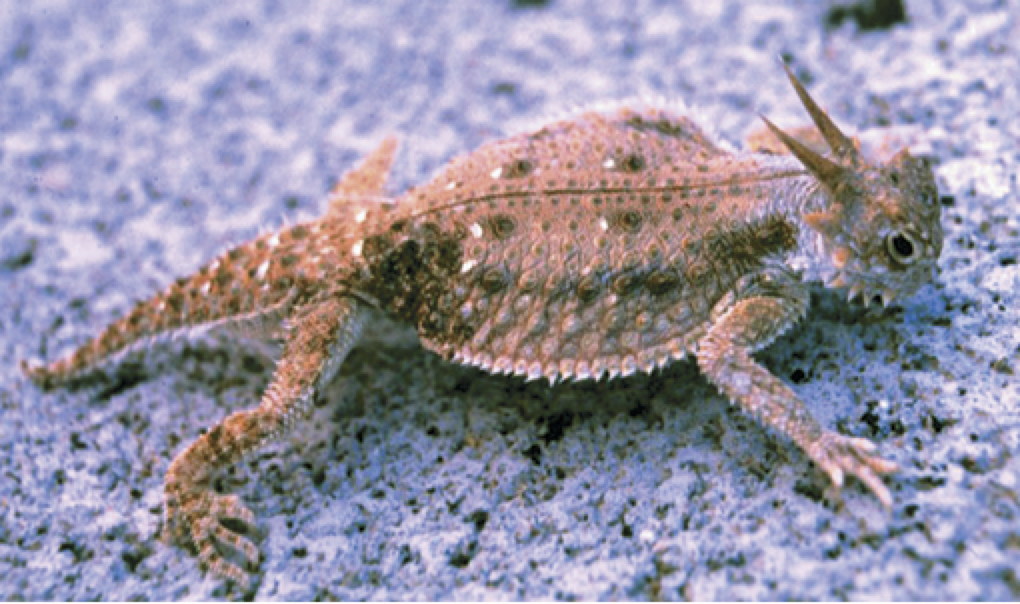
\includegraphics[keepaspectratio]{images/HornAlive.png}}

}

\subcaption{\label{fig-alive}Lézard cornu vivant}

\end{minipage}%
%
\begin{minipage}[t]{0.33\linewidth}

\centering{

\pandocbounded{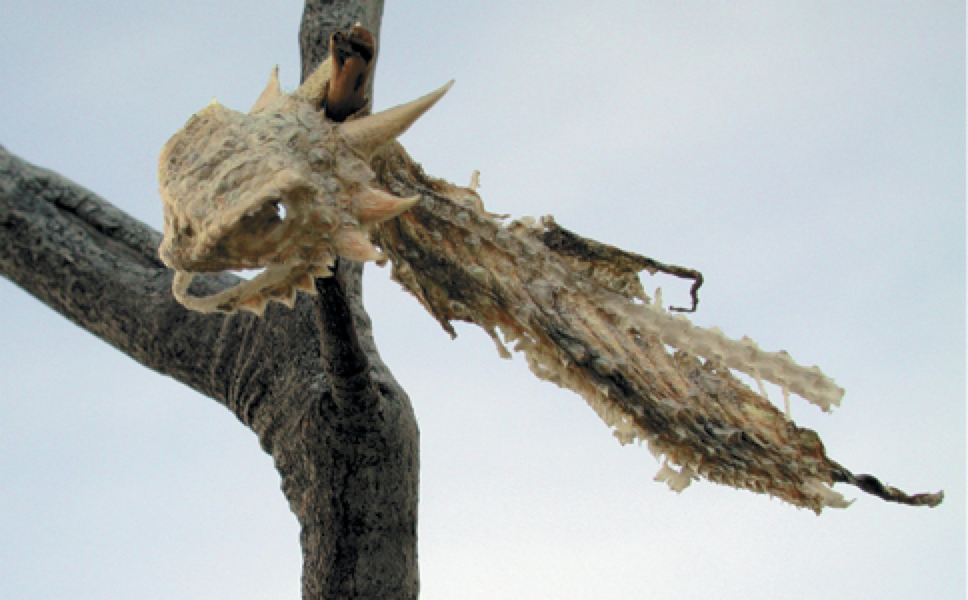
\includegraphics[keepaspectratio]{images/HornDead.png}}

}

\subcaption{\label{fig-dead}Lézard cornu mort}

\end{minipage}%
%
\begin{minipage}[t]{0.33\linewidth}

\centering{

\pandocbounded{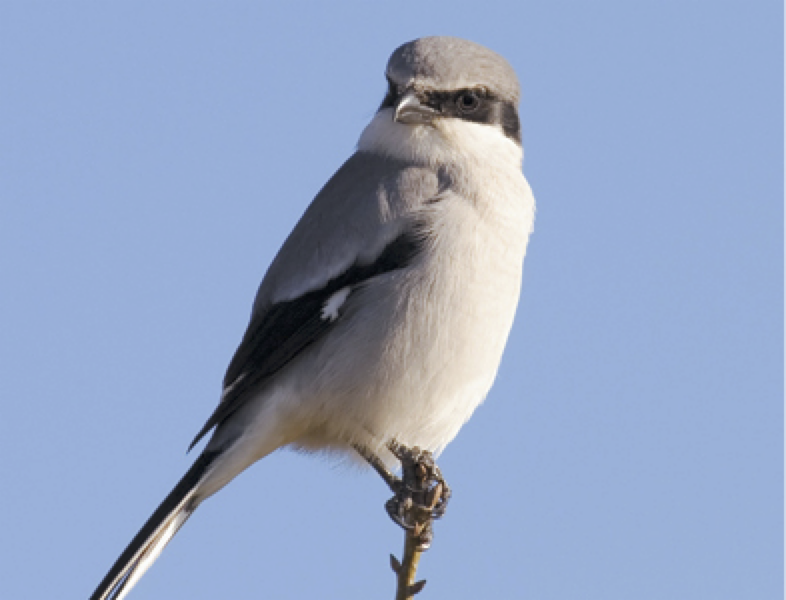
\includegraphics[keepaspectratio]{images/HornPredator.png}}

}

\subcaption{\label{fig-predator}Pie grièche}

\end{minipage}%

\caption{\label{fig-HornedLizards}Le lézard cornu et son prédateur}

\end{figure}%

Nous disposons donc de 2 groupes indépendants : chaque lézard n'a fourni
qu'une valeur de longueur de cornes, et chaque lézard n'appartient qu'à
un groupe, vivant ou mort. Nous sommes donc dans la situation typique de
la comparaison de moyennes de 2 populations avec des données
indépendantes. Avant de procéder aux tests, et comme toujours, nous
allons commencer par importer et mettre en forme les données (si
besoin), puis nous devrons explorer les données, à l'aide d'une part
d'indices statistiques de position, de dispersion et d'incertitude et
d'autre part de représentations graphiques pertinentes. Enfin, nous
vérifierons les conditions d'application du test paramétrique de Student
avant de réaliser ce test si les conditions d'application sont remplies,
ou son équivalent non paramétrique si elles ne le sont pas.

\section{Importation et mise en forme des
données}\label{importation-et-mise-en-forme-des-donnuxe9es-2}

Les données de cette étude sont stockées dans
\href{data/HornedLizards.csv}{le fichier \texttt{HornedLizards.csv}}.
Importez ces données dans un objet nommé \texttt{Lizard\_raw} et
examinez le tableau obtenu.

\begin{Shaded}
\begin{Highlighting}[]
\NormalTok{Lizard\_raw}
\end{Highlighting}
\end{Shaded}

\begin{verbatim}
# A tibble: 185 x 2
   squamosalHornLength Survival
                 <dbl> <chr>   
 1                25.2 living  
 2                26.9 living  
 3                26.6 living  
 4                25.6 living  
 5                25.7 living  
 6                25.9 living  
 7                27.3 living  
 8                25.1 living  
 9                30.3 living  
10                25.6 living  
# i 175 more rows
\end{verbatim}

\begin{Shaded}
\begin{Highlighting}[]
\FunctionTok{View}\NormalTok{(Lizard\_raw)}
\end{Highlighting}
\end{Shaded}

On constate ici 3 choses :

\begin{enumerate}
\def\labelenumi{\arabic{enumi}.}
\tightlist
\item
  la variable \texttt{Survival} devrait être un facteur.
\item
  le nom de la première colonne (\texttt{squamosalHornLength}), qui
  contient les mesures des longueurs de cornes, est bien trop long.
\item
  pour l'un des lézards vivants, la mesure de longueur des cornes est
  manquante. Nous allons donc retirer cet individu pour éviter les
  messages d'erreurs par la suite.
\end{enumerate}

Nous pouvons facilement réaliser les 3 modifications d'un coup, et
stokcer le résultat dans un nouveau tableau \texttt{Lizard} :

\begin{Shaded}
\begin{Highlighting}[]
\NormalTok{Lizard }\OtherTok{\textless{}{-}}\NormalTok{ Lizard\_raw }\SpecialCharTok{|\textgreater{}}
  \FunctionTok{mutate}\NormalTok{(}\AttributeTok{Survival =} \FunctionTok{factor}\NormalTok{(Survival)) }\SpecialCharTok{|\textgreater{}}
  \FunctionTok{rename}\NormalTok{(}\AttributeTok{Horn\_len =}\NormalTok{ squamosalHornLength) }\SpecialCharTok{|\textgreater{}}
  \FunctionTok{filter}\NormalTok{(}\SpecialCharTok{!}\FunctionTok{is.na}\NormalTok{(Horn\_len))}

\NormalTok{Lizard}
\end{Highlighting}
\end{Shaded}

\begin{verbatim}
# A tibble: 184 x 2
   Horn_len Survival
      <dbl> <fct>   
 1     25.2 living  
 2     26.9 living  
 3     26.6 living  
 4     25.6 living  
 5     25.7 living  
 6     25.9 living  
 7     27.3 living  
 8     25.1 living  
 9     30.3 living  
10     25.6 living  
# i 174 more rows
\end{verbatim}

Ce tableau est bien un tableau rangé, au format long : chaque colonne
contient une unique variable (\texttt{Horn\_len} : longueur des cornes,
\texttt{Survival} : groupe de l'individu mesuré, vivant ou mort), et
chaque ligne contient les informations d'un unique individu.

Ici, il ne serait pas correct de présenter les données au format large.
il nous faudrait en effet une colonne pour chaque groupe, lézard vivant
et lézard mort, mais puisque les données de ces 2 groupes sont
indépendantes, nous aurions 2 problèmes :

\begin{enumerate}
\def\labelenumi{\arabic{enumi}.}
\tightlist
\item
  si le nombre d'individu n'est pas le même dans les 2 groupes, les deux
  colonnes n'auraient pas la même longueur. C'est impossible dans
  \texttt{RStudio}, et le logiciel remplierait donc la colonne la plus
  courte de NAs pour y remédier.
\item
  les lignes de cet hypothétique tableau large ne correspondraient plus
  à des observations uniques. Chaque ligne renseignerait en effet sur
  les mesures de 2 individus distincts, un vivant et un mort.
\end{enumerate}

Lorsque vous disposez de données appartenant à des groupes indépendants,
il faut donc toujours travailler avec un tableau rangé, nécessairement
au format long.

\section{Exploration statistique des
données}\label{exploration-statistique-des-donnuxe9es-1}

Comme dans le Chapitre~\ref{sec-moy2} sur les données appariées, les
statistiques descriptives doivent ici être réalisées pour chaque groupe
d'individus, et non tous groupes confondus. Ici, le plus simple est
d'utiliser la fonction \texttt{skim()} sur les données groupées par
niveau du facteur \texttt{Survival} (avec la fonction
\texttt{group\_by()}) :

\begin{Shaded}
\begin{Highlighting}[]
\NormalTok{Lizard }\SpecialCharTok{|\textgreater{}}
  \FunctionTok{group\_by}\NormalTok{(Survival) }\SpecialCharTok{|\textgreater{}}
  \FunctionTok{skim}\NormalTok{()}
\end{Highlighting}
\end{Shaded}

\begin{verbatim}
-- Data Summary ------------------------
                           Values                      
Name                       group_by(Lizard, Survival...
Number of rows             184                         
Number of columns          2                           
_______________________                                
Column type frequency:                                 
  numeric                  1                           
________________________                               
Group variables            Survival                    

-- Variable type: numeric ------------------------------------------------------
  skim_variable Survival n_missing complete_rate mean   sd   p0  p25  p50  p75
1 Horn_len      killed           0             1 22.0 2.71 15.2 21.1 22.2 23.8
2 Horn_len      living           0             1 24.3 2.63 13.1 23   24.6 26  
  p100 hist 
1 26.7 ▂▂▇▇▃
2 30.3 ▁▁▅▇▂
\end{verbatim}

On constate ici qu'il n'y a pas de données manquantes
(\texttt{n\_missing} = 0 dans les deux groupes). La moyenne des
longueurs de cornes est plus grande chez les lézards vivants
(\(\bar{x}_{living} = 24.3\) mm) que chez les lézards retrouvés morts
(\(\bar{x}_{killed} = 22.0\)), de plus de 2 millimètres. On retrouve
cette tendance pour les médianes, ainsi que pour les premiers et
troisièmes quartiles. En revanche, les écarts-types des 2 groupes sont
proches, et celui du groupe \texttt{living} est très légèrement plus
faible (0.08 mm) que celui du groupe \texttt{killed}.

Enfin, les histogrammes très simplifiés fournis laissent penser que les
données de chaque groupe ne s'écartent pas trop fortement d'une courbe
en cloche.

Outre ces informations sur les ordres de grandeurs observés dans chaque
groupe de lézards pour les indices de \textbf{position} (moyennes,
médianes et quartiles), et de \textbf{dispersion} (écarts-types et
histogrammes), la fonction \texttt{skim()} ne fournit pas les effectifs
observés dans chaque groupe. On sait qu'il y a en tout 184 individus,
mais on ne sait pas comment ils se répartissent dans les 2 groupes de
lézards. Pour le déterminer, on peut utiliser une fonction décrite plus
tôt, la fonction \texttt{count()} :

\begin{Shaded}
\begin{Highlighting}[]
\NormalTok{Lizard }\SpecialCharTok{|\textgreater{}}
  \FunctionTok{count}\NormalTok{(Survival)}
\end{Highlighting}
\end{Shaded}

\begin{verbatim}
# A tibble: 2 x 2
  Survival     n
  <fct>    <int>
1 killed      30
2 living     154
\end{verbatim}

On peut obtenir la même information avec la fonction
\texttt{summarise()} et son argument \texttt{.by}, et la fonction
\texttt{n()} :

\begin{Shaded}
\begin{Highlighting}[]
\NormalTok{Lizard }\SpecialCharTok{|\textgreater{}} 
  \FunctionTok{summarize}\NormalTok{(}\AttributeTok{Effectif =} \FunctionTok{n}\NormalTok{(), }\AttributeTok{.by =}\NormalTok{ Survival)}
\end{Highlighting}
\end{Shaded}

\begin{verbatim}
# A tibble: 2 x 2
  Survival Effectif
  <fct>       <int>
1 living        154
2 killed         30
\end{verbatim}

On constate ici que les tailles d'échantillons sont très différentes.
C'est normal compte tenu de la difficulté de repérer des individus morts
dans la nature, et ce n'est pas gênant pour nos analyses puisque la
taille des deux échantillons reste élevée.

Enfin, on peut calculer des indices d'incertitude. C'est d'autant plus
important qu'il est difficile de se faire une idée de la signification
d'une différence moyenne de longueur de cornes de 2 millimètres. Est-ce
important ou négligeable ? Est-ce que ces estimations sont précises ou
non ? Comme dans les chapitres précédents, nous allons calculer les
intervalles de confiance à 95\% de la moyenne de chaque groupe :

\begin{Shaded}
\begin{Highlighting}[]
\NormalTok{Lizard }\SpecialCharTok{|\textgreater{}} 
  \FunctionTok{reframe}\NormalTok{(}\FunctionTok{mean\_cl\_normal}\NormalTok{(Horn\_len), }\AttributeTok{.by =}\NormalTok{ Survival)}
\end{Highlighting}
\end{Shaded}

\begin{verbatim}
# A tibble: 2 x 4
  Survival     y  ymin  ymax
  <fct>    <dbl> <dbl> <dbl>
1 living    24.3  23.9  24.7
2 killed    22.0  21.0  23.0
\end{verbatim}

La colonne \texttt{y} nous présente à nouveau la moyenne de chaque
groupe, la colonne \texttt{ymin} contient les bornes inférieures des
intervalles de confiance à 95\%, et la colonne \texttt{ymax} les bornes
supérieures. On constate ici que les intervalles de confiance à 95\% des
longueurs de cornes des 2 groupes ne se chevauchent pas du tout : la
borne inférieure du groupe \texttt{living} est au-dessus de la borne
supérieure du groupe \texttt{killed}. Autrement dit, dans la population
générale, la longueur moyenne des cornes chez les lézards vivants a de
bonnes chances de se trouver dans l'intervalle {[}23.9 ; 24.7{]}
millimètres, alors qu'elle a de bonnes chances de se trouver dans
l'intervalle {[}21 ; 23{]} millimètres chez les lézards morts. La
différence de moyennes entre ces 2 groupes vaut donc probablement entre
0.9 millimètres au moins, et 3.7 millimètres au plus. Le test
statistique que nous ferons ensuite devrait donc confirmer que ces
différences sont significatives, autrement dit, qu'elles ne sont pas
liées au simple hasard de l'échantillonnage.

\section{Exploration graphique des
données}\label{exploration-graphique-des-donnuxe9es-1}

Comme toujours, nous pouvons réaliser plusieurs types de graphiques pour
en apprendre plus sur \textbf{la distribution des données} dans les deux
groupes. Si nous faisons un nuage de points, il est évidemment
impossible ici de relier les points deux à deux. Non seulement cela
n'aurait aucun sens puisque les échantillons sont indépendants, mais en
outre, nous ne disposons pas du même nombre d'individus dans les 2
échantillons. Nous nous contenterons donc da faire un stripchart.

\subsection{Avec un stripchart}\label{avec-un-stripchart-1}

\begin{Shaded}
\begin{Highlighting}[]
\NormalTok{Lizard }\SpecialCharTok{|\textgreater{}}
  \FunctionTok{ggplot}\NormalTok{(}\FunctionTok{aes}\NormalTok{(}\AttributeTok{x =}\NormalTok{ Survival, }\AttributeTok{y =}\NormalTok{ Horn\_len)) }\SpecialCharTok{+}
  \FunctionTok{geom\_jitter}\NormalTok{(}\AttributeTok{height =} \DecValTok{0}\NormalTok{, }\AttributeTok{width =} \FloatTok{0.2}\NormalTok{, }\AttributeTok{alpha =} \FloatTok{0.5}\NormalTok{) }\SpecialCharTok{+}
  \FunctionTok{labs}\NormalTok{(}\AttributeTok{x =} \StringTok{"Groupe de lézards"}\NormalTok{,}
       \AttributeTok{y =} \StringTok{"Longueur des cornes (mm)"}\NormalTok{,}
       \AttributeTok{title =} \StringTok{"Visualisation des longueurs}\SpecialCharTok{\textbackslash{}n}\StringTok{de cornes du lézard cornu"}\NormalTok{)}
\end{Highlighting}
\end{Shaded}

\begin{center}
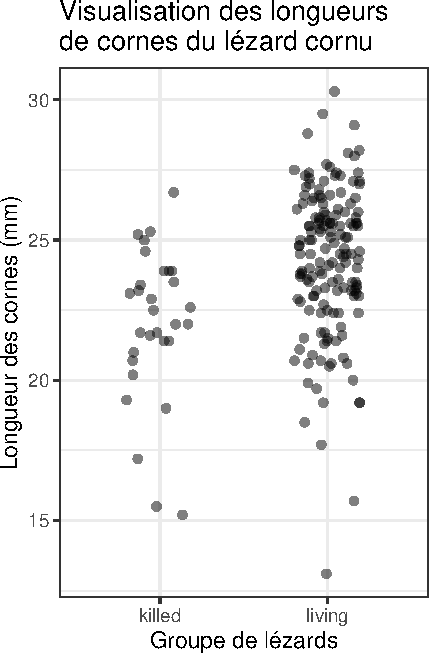
\includegraphics[width=0.5\linewidth,height=\textheight,keepaspectratio]{03-TwoSampleTests_files/figure-pdf/unnamed-chunk-11-1.pdf}
\end{center}

Ce premier graphique permet de visualiser très clairement les
différences de tailles d'échantillons entre les deux groupes. Il permet
également de voir que l'étendue des longueurs de cornes est plus
importante dans le groupe des individus vivants que dans celui des
individus morts. En outre, le nuage de points des vivants semble être
plus haut sur l'axe des \texttt{y} que celui des morts, confirmant les
statistiques descriptives qui montraient des tailles de cornes en
moyenne plus importantes dans le groupe des vivants.

\subsection{Avec des histogrammes facettés}\label{sec-histofacet}

\begin{Shaded}
\begin{Highlighting}[]
\NormalTok{Lizard }\SpecialCharTok{|\textgreater{}}
  \FunctionTok{ggplot}\NormalTok{(}\FunctionTok{aes}\NormalTok{(}\AttributeTok{x =}\NormalTok{ Horn\_len)) }\SpecialCharTok{+}
  \FunctionTok{geom\_histogram}\NormalTok{(}\AttributeTok{bins =} \DecValTok{15}\NormalTok{, }\AttributeTok{fill =} \StringTok{"firebrick2"}\NormalTok{, }\AttributeTok{color =} \StringTok{"grey20"}\NormalTok{, }\AttributeTok{alpha =} \FloatTok{0.5}\NormalTok{)}\SpecialCharTok{+}
  \FunctionTok{geom\_rug}\NormalTok{() }\SpecialCharTok{+}
  \FunctionTok{facet\_wrap}\NormalTok{(}\SpecialCharTok{\textasciitilde{}}\NormalTok{Survival, }\AttributeTok{ncol =} \DecValTok{1}\NormalTok{, }\AttributeTok{scales =} \StringTok{"free\_y"}\NormalTok{) }\SpecialCharTok{+}
  \FunctionTok{labs}\NormalTok{(}\AttributeTok{x =} \StringTok{"Longueur des cornes (mm)"}\NormalTok{,}
       \AttributeTok{y =} \StringTok{"Fréquence"}\NormalTok{,}
       \AttributeTok{title =} \StringTok{"Distribution de la longueur des cornes dans 2 groupes de lézards cornus"}\NormalTok{,}
       \AttributeTok{subtitle =} \StringTok{"nb morts : 30, nb vivants : 154"}\NormalTok{)}
\end{Highlighting}
\end{Shaded}

\pandocbounded{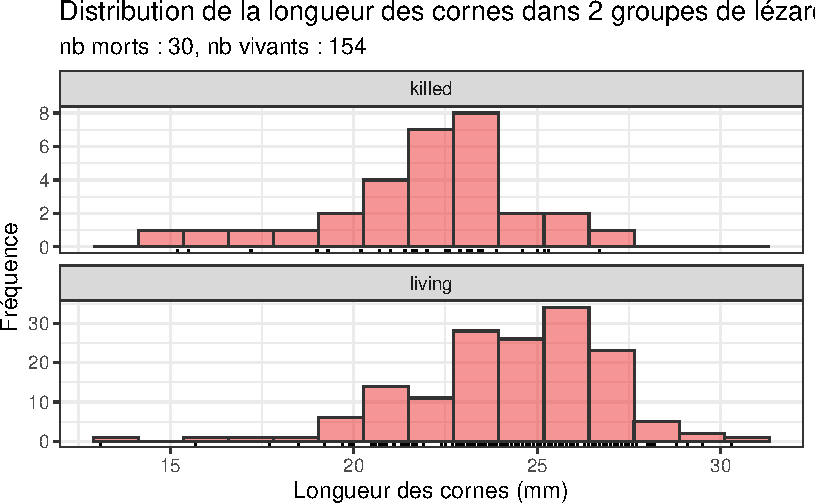
\includegraphics[keepaspectratio]{03-TwoSampleTests_files/figure-pdf/unnamed-chunk-12-1.pdf}}

Notez ici l'utilisation de l'argument \texttt{scales\ =\ "free\_y"} dans
la fonction \texttt{facet\_wrap()}. Cet argument permet de ne pas
imposer la même échelle pour l'axe des ordonnées des 2 graphiques. Ce
choix est ici pertinent puisque les effectifs des 2 groupes sont très
différents. Faîtes un essai sans cet argument pour voir la différence.
Il est en revanche important de conserver le même axe des \texttt{x}
afin de faciliter la comparaison des 2 groupes.

Cette visualisation nous montre que les données doivent suivre à peu
près une distribution Normale dans les 2 groupes, et que globalement la
longueur des cornes semble légèrement plus élevée dans le groupe des
vivants (avec un mode autour de 25-26 mm) que dans le groupes des morts
(avec un mode autour de 23-24 mm). L'étendue des données semble
légèrement plus grande dans le groupe des vivants, mais cela n'est
peut-être dû qu'à la différence marquée des tailles d'échantillons.

\subsection{Avec des diagrammes de densité
facettés}\label{sec-densfacet}

\begin{Shaded}
\begin{Highlighting}[]
\NormalTok{Lizard }\SpecialCharTok{|\textgreater{}}
  \FunctionTok{ggplot}\NormalTok{(}\FunctionTok{aes}\NormalTok{(}\AttributeTok{x =}\NormalTok{ Horn\_len)) }\SpecialCharTok{+}
  \FunctionTok{geom\_density}\NormalTok{(}\AttributeTok{fill =} \StringTok{"firebrick2"}\NormalTok{, }\AttributeTok{alpha =} \FloatTok{0.5}\NormalTok{) }\SpecialCharTok{+}
  \FunctionTok{geom\_rug}\NormalTok{() }\SpecialCharTok{+}
  \FunctionTok{facet\_wrap}\NormalTok{(}\SpecialCharTok{\textasciitilde{}}\NormalTok{Survival, }\AttributeTok{ncol =} \DecValTok{1}\NormalTok{, }\AttributeTok{scales =} \StringTok{"free\_y"}\NormalTok{) }\SpecialCharTok{+}
  \FunctionTok{labs}\NormalTok{(}\AttributeTok{x =} \StringTok{"Longueur des cornes (mm)"}\NormalTok{,}
       \AttributeTok{y =} \StringTok{"Densité"}\NormalTok{,}
       \AttributeTok{title =} \StringTok{"Distribution de la longueur des cornes dans 2 groupes de lézards cornus"}\NormalTok{,}
       \AttributeTok{subtitle =} \StringTok{"nb morts : 30, nb vivants : 154"}\NormalTok{)}
\end{Highlighting}
\end{Shaded}

\pandocbounded{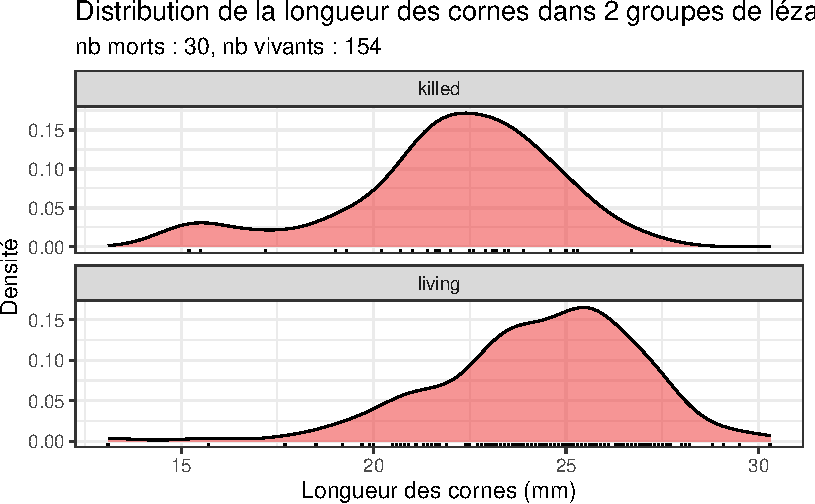
\includegraphics[keepaspectratio]{03-TwoSampleTests_files/figure-pdf/unnamed-chunk-13-1.pdf}}

Les diagrammes de densité ressemblent ici beaucoup aux histogrammes.
C'est normal car la taille des échantillons est importante (30 et 154
pour les groupes \texttt{killed} et \texttt{living} respectivement).
C'était moins vrais dans les chapitres précédents car les tailles
d'échantillons étaient plus faibles, et la forme des histogrammes
dépendait alors beaucoup du nombre de classes que l'on choisissait de
représenter. Avec des échantillons de grande taille (n ≥ 30), c'est
moins problématique.

En général, il est donc inutile de faire à la fois les histogrammes et
les diagrammes de densité. Choisissez l'un ou l'autre selon vos
préférences et la situation.

\subsection{Avec des boites à
moustaches}\label{avec-des-boites-uxe0-moustaches}

\begin{Shaded}
\begin{Highlighting}[]
\NormalTok{Lizard }\SpecialCharTok{|\textgreater{}}
  \FunctionTok{ggplot}\NormalTok{(}\FunctionTok{aes}\NormalTok{(}\AttributeTok{x =}\NormalTok{ Survival, }\AttributeTok{y =}\NormalTok{ Horn\_len)) }\SpecialCharTok{+}
  \FunctionTok{geom\_boxplot}\NormalTok{(}\AttributeTok{notch =} \ConstantTok{TRUE}\NormalTok{) }\SpecialCharTok{+}
  \FunctionTok{labs}\NormalTok{(}\AttributeTok{x =} \StringTok{"Groupe de lézards"}\NormalTok{,}
       \AttributeTok{y =} \StringTok{"Longueur des cornes (mm)"}\NormalTok{,}
       \AttributeTok{title =} \StringTok{"Comparaison de 2 groupes}\SpecialCharTok{\textbackslash{}n}\StringTok{de lézards cornus"}\NormalTok{,}
       \AttributeTok{subtitle =} \StringTok{"nb morts : 30, nb vivants : 154"}\NormalTok{)}
\end{Highlighting}
\end{Shaded}

\begin{center}
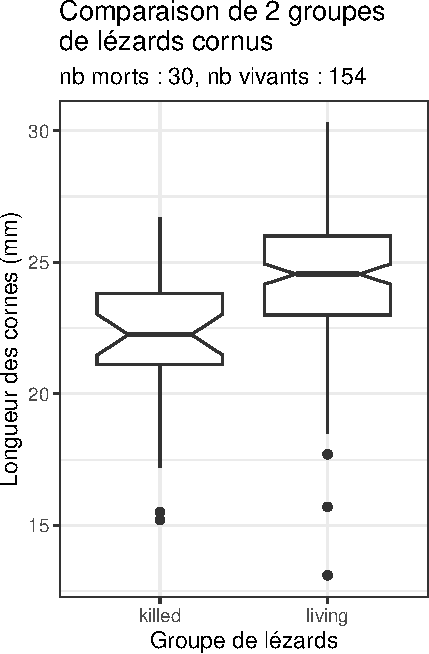
\includegraphics[width=0.5\linewidth,height=\textheight,keepaspectratio]{03-TwoSampleTests_files/figure-pdf/unnamed-chunk-14-1.pdf}
\end{center}

Nous visualisons ici encore plus clairement que sur les histogrammes le
fait que les longueurs de cornes des individus vivants sont légèrement
plus longues que celles des individus morts. D'ailleurs, puisque les
intervalles de confiance à 95\% des médianes des 2 groupes (les
encoches) ne se chevauchent pas, un test de comparaison des moyennes
devrait logiquement conclure à une différence significative en faveur
des individus vivants. On peut également noter que la largeur de
l'encoche pour les individus morts est plus importante que celle des
vivants. Cela traduit une incertitude plus grande autour de la médiane
estimée dans le groupe des individus morts. C'est tout à fait logique
compte tenu des effectifs plus faibles dans ce groupe.

Enfin, il est tout à fait possible de représenter sur le même graphique
les boîtes à moustaches et les données brutes sous forme de stripchart.
On a ainsi à la fois (i) une visualisation simplifiée de la position et
de la dispersion des données avec les boîtes à moustache, et (ii) accès
à l'ensemble des données brutes, ce qui permet parfois de voir des
structures invisibles sur les boîtes à moustaches (regroupement de
points par exemples). Afin de ne pas dupliquer les valeurs les plus
extrêmes du jeu de données, nous indiquerons à \texttt{geom\_boxplot()}
de ne pas afficher les outliers sur le graphique : tous les points
seront en effet déjà affichés par \texttt{geom\_jitter()} :

\begin{Shaded}
\begin{Highlighting}[]
\NormalTok{Lizard }\SpecialCharTok{|\textgreater{}}
  \FunctionTok{ggplot}\NormalTok{(}\FunctionTok{aes}\NormalTok{(}\AttributeTok{x =}\NormalTok{ Survival, }\AttributeTok{y =}\NormalTok{ Horn\_len, }\AttributeTok{fill =}\NormalTok{ Survival)) }\SpecialCharTok{+}
  \FunctionTok{geom\_boxplot}\NormalTok{(}\AttributeTok{notch =} \ConstantTok{TRUE}\NormalTok{, }\AttributeTok{color =} \StringTok{"grey20"}\NormalTok{, }\AttributeTok{alpha =} \FloatTok{0.2}\NormalTok{,}
               \AttributeTok{outlier.color =} \ConstantTok{NA}\NormalTok{, }\AttributeTok{show.legend =} \ConstantTok{FALSE}\NormalTok{) }\SpecialCharTok{+}
  \FunctionTok{geom\_jitter}\NormalTok{(}\AttributeTok{height =} \DecValTok{0}\NormalTok{, }\AttributeTok{width =} \FloatTok{0.2}\NormalTok{, }\AttributeTok{alpha =} \FloatTok{0.4}\NormalTok{, }\AttributeTok{shape =} \DecValTok{21}\NormalTok{,}
              \AttributeTok{show.legend =} \ConstantTok{FALSE}\NormalTok{, }\AttributeTok{size =} \FloatTok{0.8}\NormalTok{) }\SpecialCharTok{+}
  \FunctionTok{labs}\NormalTok{(}\AttributeTok{x =} \StringTok{"Groupe de lézards"}\NormalTok{,}
       \AttributeTok{y =} \StringTok{"Longueur des cornes (mm)"}\NormalTok{,}
       \AttributeTok{title =} \StringTok{"Comparaison de 2 groupes}\SpecialCharTok{\textbackslash{}n}\StringTok{de lézards cornus"}\NormalTok{,}
       \AttributeTok{subtitle =} \StringTok{"nb morts : 30, nb vivants : 154"}\NormalTok{) }\SpecialCharTok{+}
  \FunctionTok{scale\_fill\_manual}\NormalTok{(}\AttributeTok{values =} \FunctionTok{c}\NormalTok{(}\StringTok{"purple3"}\NormalTok{, }\StringTok{"royalblue2"}\NormalTok{))}
\end{Highlighting}
\end{Shaded}

\begin{center}
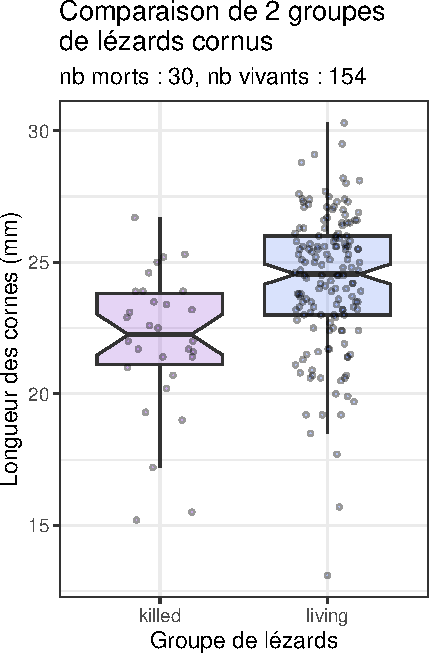
\includegraphics[width=0.5\linewidth,height=\textheight,keepaspectratio]{03-TwoSampleTests_files/figure-pdf/unnamed-chunk-15-1.pdf}
\end{center}

\section{Le test paramétrique}\label{le-test-paramuxe9trique-2}

Le test paramétrique le plus puissant que nous puissions faire pour
comparer la moyenne de 2 populations est le test de Student. Ce test
étant paramétrique, nous devons nous assurer que ses conditions
d'application sont vérifiées avant de pouvoir le réaliser.

\subsection{Conditions d'application}\label{sec-robust}

Les conditions d'application de ce test sont au nombre de 3 :

\begin{enumerate}
\def\labelenumi{\arabic{enumi}.}
\tightlist
\item
  Chacun des deux échantillons est issu d'un échantillonnage aléatoire
  de la population générale. Comme toujours, en l'absence d'indication
  contraire, on considère que cette condition est toujours vérifiée.
\item
  La variable numérique étudiée est distribuée normalement dans les deux
  populations. Il nous faudra donc faire deux tests de Shapiro-Wilk, un
  pour chaque échantillon.
\item
  La variance de la variable numérique étudiée est la même dans les deux
  populations. C'est ce que l'on appelle l'homoscédasticité.
\end{enumerate}

En réalité, le test du \(t\) de Student sur deux échantillons
indépendants est assez robuste face au non respect de cette troisième
condition d'application. Cela signifie que si cette troisième condition
d'application n'est pas strictement vérifiée, les résultats du tests
peuvent malgré tout rester valides. Lorsque les 2 échantillons comparés
ont des tailles supérieures ou égales à 30, ce test fonctionne bien même
si l'écart-type d'un groupe est jusqu'à 3 fois supérieur ou inférieur à
l'écart-type du second groupe, à condition que la taille des 2
échantillons soit proche (ce qui n'est pas le cas ici !). En revanche,
si les écart-types diffèrent de plus d'un facteur 3, ou si les tailles
d'échantillons sont très différentes, le test du \(t\) de Student ne
devrait pas être utilisé. De même, si la taille des échantillons est
inférieure à 30 et que les variances ne sont pas homogènes, ce test ne
devrait pas être réalisé. En conclusion, les résultats du test du \(t\)
de Student à deux échantillons indépendants peuvent rester valides si la
troisième condition d'homoscédasticité n'est pas respectée, mais dans
certains cas seulement.

Le test du \(t\) de Student sur deux échantillons indépendants est
également assez robuste face à des écarts mineurs à la distribution
Normale, tant que la forme des deux distributions comparées reste
similaire et unimodale. En outre, la robustesse de ce test augmente avec
la taille des échantillons.

\begin{tcolorbox}[enhanced jigsaw, arc=.35mm, bottomrule=.15mm, bottomtitle=1mm, breakable, colback=white, colbacktitle=quarto-callout-tip-color!10!white, colframe=quarto-callout-tip-color-frame, coltitle=black, left=2mm, leftrule=.75mm, opacityback=0, opacitybacktitle=0.6, rightrule=.15mm, title=\textcolor{quarto-callout-tip-color}{\faLightbulb}\hspace{0.5em}{Robustesse}, titlerule=0mm, toprule=.15mm, toptitle=1mm]

La robustesse d'un tests statistique est sa capacité à rester valide
même lorsque certaines de ses conditions d'application ne sont pas
parfaitement respectées. Plus un test est robuste, plus il est capable
de supporter des ``entorses'' importantes à ses conditions
d'application.\}

\end{tcolorbox}

Au final, avec un peu d'habitude, même lorsque les conditions
d'application ne sont pas toutes vérifiées, on peut parfois passer
outre. Mais à ce stade, on préfère s'en tenir à des choses plus simples
et claires.

\begin{tcolorbox}[enhanced jigsaw, arc=.35mm, bottomrule=.15mm, bottomtitle=1mm, breakable, colback=white, colbacktitle=quarto-callout-warning-color!10!white, colframe=quarto-callout-warning-color-frame, coltitle=black, left=2mm, leftrule=.75mm, opacityback=0, opacitybacktitle=0.6, rightrule=.15mm, title=\textcolor{quarto-callout-warning-color}{\faExclamationTriangle}\hspace{0.5em}{La procédure à suivre}, titlerule=0mm, toprule=.15mm, toptitle=1mm]

\begin{enumerate}
\def\labelenumi{\arabic{enumi}.}
\tightlist
\item
  Faites un test de Normalité pour chacune des deux séries de données.
  Si elles suivent la loi Normale toutes les deux, passez au point 2.
  Sinon, rendez-vous au point 4.
\item
  Faites un test d'homoscédasticité (homogénéité des variances). Si les
  variances sont homogènes, passez au point 3. Sinon,rendez-vous au
  point 5.
\item
  Faite un test de comparaison des moyennes paramétrique : le test de
  Student. Examinez la \(p-\)value pour conclure, et rendez-vous au
  point 6.
\item
  Faite un test de comparaison des moyennes non paramétrique : le test
  de Wilcoxon de la somme des rangs. Examinez la \(p-\)value pour
  conclure, et rendez-vous au point 6.
\item
  Faite un test de comparaison des moyennes non paramétrique : le test
  \(t\) de Welch. Examinez la \(p-\)value pour conclure, et rendez-vous
  au point 6.
\item
  Si la \(p-\)value est supérieure à \(\alpha\), on ne peut pas rejeter
  l'hypothèse nulle et on conclut alors à une absence de différence
  significative entre les 2 populations. À l'inverse, si la \(p-\)value
  est inférieure ou égale à \(\alpha\), on rejette l'hypothèse nulle et
  on valide l'hypothèse alternative. Les deux populations ont des
  moyennes significativement différentes, et pour savoir laquelle est
  supérieure ou inférieure à l'autre, on revient aux estimations des
  moyennes et des intervalles de confiances à 95\%, calculés dans la
  partie consacrée aux statistiques descriptives.
\end{enumerate}

\end{tcolorbox}

\subsubsection{Normalité des données}\label{normalituxe9-des-donnuxe9es}

Nous commençons donc par tester la Normalité des 2 populations dont sont
issus les échantillons, c'est le point 1 de la procédure détaillée
ci-dessus. Pour les individus morts, les hypothèses sont les suivantes :

\begin{itemize}
\tightlist
\item
  H\(_0\) : la taille des cornes suit une distribution Normale dans la
  population des lézards cornus morts.
\item
  H\(_1\) : la taille des cornes ne suit pas une distribution Normale
  dans la population des lézards cornus morts.
\end{itemize}

\begin{Shaded}
\begin{Highlighting}[]
\NormalTok{Lizard }\SpecialCharTok{|\textgreater{}}
  \FunctionTok{filter}\NormalTok{(Survival }\SpecialCharTok{==} \StringTok{"killed"}\NormalTok{) }\SpecialCharTok{|\textgreater{}}
  \FunctionTok{pull}\NormalTok{(Horn\_len) }\SpecialCharTok{|\textgreater{}}
  \FunctionTok{shapiro.test}\NormalTok{()}
\end{Highlighting}
\end{Shaded}

\begin{verbatim}

    Shapiro-Wilk normality test

data:  pull(filter(Lizard, Survival == "killed"), Horn_len)
W = 0.93452, p-value = 0.06482
\end{verbatim}

\begin{quote}
La \(p\)-value est supérieure à \(\alpha = 0.05\), donc on ne peut pas
rejeter l'hypothèse nulle de normalité pour la taille des cornes de la
population des lézards cornus morts (test de Shapiro-Wilk, \(W = 0.93\),
\(p = 0.065\)).
\end{quote}

Pour les individus vivants :

\begin{itemize}
\tightlist
\item
  H\(_0\) : la taille des cornes suit une distribution Normale dans la
  population des lézards cornus vivants.
\item
  H\(_1\) : la taille des cornes ne suit pas une distribution Normale
  dans la population des lézards cornus vivants.
\end{itemize}

\begin{Shaded}
\begin{Highlighting}[]
\NormalTok{Lizard }\SpecialCharTok{|\textgreater{}}
  \FunctionTok{filter}\NormalTok{(Survival }\SpecialCharTok{==} \StringTok{"living"}\NormalTok{) }\SpecialCharTok{|\textgreater{}}
  \FunctionTok{pull}\NormalTok{(Horn\_len) }\SpecialCharTok{|\textgreater{}}
  \FunctionTok{shapiro.test}\NormalTok{()}
\end{Highlighting}
\end{Shaded}

\begin{verbatim}

    Shapiro-Wilk normality test

data:  pull(filter(Lizard, Survival == "living"), Horn_len)
W = 0.96055, p-value = 0.0002234
\end{verbatim}

\begin{quote}
La \(p\)-value est inférieure à \(\alpha = 0.05\), donc on rejette
l'hypothèse nulle de normalité pour la taille des cornes de la
population des lézards cornus vivants (test de Shapiro-Wilk,
\(W = 0.96\), \(p < 0.001\)).
\end{quote}

L'une des 2 séries de données ne suit pas la loi Normale, nous sommes
donc censés passer directement au point 4 de la procédure.

Toutefois, si l'on examine les histogrammes
(Section~\ref{sec-histofacet}) ou les diagrammes de densité
(Section~\ref{sec-densfacet}) des 2 échantillons, on constate que la
forme des distributions des 2 séries de données est très proche. Pour
les 2 échantillons, la distribution est en effet uni-modale, avec une
asymétrie gauche assez marquée (une longue queue de distribution du côté
gauche). La forme des distributions étant similaire (on parle bien de la
forme des histogrammes et non de la position du pic), et les
histogrammes étant proches de la forme typique d'une courbe en cloche,
le test de Student devrait rester valide car il est robuste dans cette
situation. Ici, pour l'exemple, on va donc passer au point 2 de la
procédure. Notez toutefois que passer directement au point 4 de la
procédure serait tout à fait correct : on ne pourrait rien vous
reprocher si vous passez directement au test non paramétrique de
comparaison des moyennes lorsque vous constatez que l'une des 2 séries
de données ne suit pas la distribution Normale.

\subsubsection{Homogénéité des
variances}\label{homoguxe9nuxe9ituxe9-des-variances}

Le test le plus simple pour comparer la variance de 2 populations est le
test \(F\) :

\begin{itemize}
\tightlist
\item
  H\(_0\) : la variance des 2 populations est égale, leur ratio vaut 1
  \(\left(\frac{\sigma^2_{killed}}{\sigma^2_{living}} = 1\right)\).
\item
  H\(_1\) : la variance des 2 populations est différente, leur ratio ne
  vaut pas 1
  \(\left(\frac{\sigma^2_{killed}}{\sigma^2_{living}} \neq 1\right)\).
\end{itemize}

\begin{Shaded}
\begin{Highlighting}[]
\FunctionTok{var.test}\NormalTok{(Horn\_len }\SpecialCharTok{\textasciitilde{}}\NormalTok{ Survival, }\AttributeTok{data =}\NormalTok{ Lizard)}
\end{Highlighting}
\end{Shaded}

\begin{verbatim}

    F test to compare two variances

data:  Horn_len by Survival
F = 1.0607, num df = 29, denom df = 153, p-value = 0.7859
alternative hypothesis: true ratio of variances is not equal to 1
95 percent confidence interval:
 0.6339331 1.9831398
sample estimates:
ratio of variances 
          1.060711 
\end{verbatim}

\begin{quote}
Ici, le ratio des variances (la variance des individus morts divisée par
la variance des individus vivants) est très proche de 1 (\(F = 1.06\),
IC 95\% : {[}0.63 ; 1.98{]}). Le test \(F\) nous montre qu'il est
impossible de rejeter H\(_0\) : au seuil \(\alpha = 0.05\), le ratio des
variances n'est pas significativement différent de 1 (ddl = 29 et 153,
\(p = 0.79\)), les variances sont homogènes.
\end{quote}

Le test de Bartlett est un autre test qui permet de comparer la variance
de plusieurs populations (2 ou plus). Lorsque le nombre de populations
est égal à 2 (comme ici), ce test est absolument équivalent au test
\(F\) ci-dessus.

\begin{itemize}
\tightlist
\item
  H\(_0\) : toutes les populations ont même variance
  (\(\sigma^2_A = \sigma^2_B = \sigma^2_C = \cdots = \sigma^2_N\)).
\item
  H\(_1\) : au moins une population a une variance différente des
  autres.
\end{itemize}

\begin{Shaded}
\begin{Highlighting}[]
\FunctionTok{bartlett.test}\NormalTok{(Horn\_len }\SpecialCharTok{\textasciitilde{}}\NormalTok{ Survival, }\AttributeTok{data =}\NormalTok{ Lizard)}
\end{Highlighting}
\end{Shaded}

\begin{verbatim}

    Bartlett test of homogeneity of variances

data:  Horn_len by Survival
Bartlett's K-squared = 0.042411, df = 1, p-value = 0.8368
\end{verbatim}

Enfin, le test de Levene (attention, le package \texttt{car} doit être
chargé) devrait être préféré la plupart du temps. Comme le test de
Bartlett, il permet de comparer la variance de plusieurs populations,
mais il est plus robuste vis à vis de la non-normalité des données.

\begin{itemize}
\tightlist
\item
  H\(_0\) : toutes les populations ont même variance
  (\(\sigma^2_A = \sigma^2_B = \sigma^2_C = \cdots = \sigma^2_N\)).
\item
  H\(_1\) : au moins une population a une variance différente des
  autres.
\end{itemize}

\begin{Shaded}
\begin{Highlighting}[]
\CommentTok{\# Le test de Levene fait partie du package car. Il doit être chargé en mémoire}
\CommentTok{\# library(car)}
\FunctionTok{leveneTest}\NormalTok{(Horn\_len }\SpecialCharTok{\textasciitilde{}}\NormalTok{ Survival, }\AttributeTok{data =}\NormalTok{ Lizard)}
\end{Highlighting}
\end{Shaded}

\begin{verbatim}
Levene's Test for Homogeneity of Variance (center = median)
       Df F value Pr(>F)
group   1  0.0035  0.953
      182               
\end{verbatim}

Ici encore, les conclusions sont les mêmes :

\begin{quote}
Il est impossible de rejeter l'hypothèse nulle d'homogénéité des
variances au seuil \(\alpha = 0.05\) (test de Levene, \(F\) = 0.004, ddl
= 1, \(p = 0.953\)).
\end{quote}

À vous de choisir lequel de ces 3 tests vous souhaitez réaliser : il est
évident qu'on ne fait jamais les 3 !

Ici, puisque l'homoscédasticité est vérifiée, on passe au point 3 de la
procédure.

\subsection{Réalisation du test et interprétation}\label{sec-student}

Puisque la taille des cornes du lézard cornu suit approximativement la
même distribution ``presque Normale'' dans les 2 populations (lézards
morts et vivants) et que ces 2 populations ont des variances homogènes,
on peut réaliser le test du \(t\) de Student sur deux échantillons
indépendants.

\begin{itemize}
\tightlist
\item
  H\(_0\) : la moyenne des 2 populations est égale, leur différence vaut
  0 (\(\mu_{killed}-\mu_{living} = 0\)).
\item
  H\(_1\) : la moyenne des 2 populations est différente, leur différence
  ne vaut pas 0 (\(\mu_{killed}-\mu_{living} \neq 0\)).
\end{itemize}

\begin{Shaded}
\begin{Highlighting}[]
\FunctionTok{t.test}\NormalTok{(Horn\_len }\SpecialCharTok{\textasciitilde{}}\NormalTok{ Survival, }\AttributeTok{data =}\NormalTok{ Lizard, }\AttributeTok{var.equal =} \ConstantTok{TRUE}\NormalTok{)}
\end{Highlighting}
\end{Shaded}

\begin{verbatim}

    Two Sample t-test

data:  Horn_len by Survival
t = -4.3494, df = 182, p-value = 2.27e-05
alternative hypothesis: true difference in means between group killed and group living is not equal to 0
95 percent confidence interval:
 -3.335402 -1.253602
sample estimates:
mean in group killed mean in group living 
            21.98667             24.28117 
\end{verbatim}

Notez bien la syntaxe :

\begin{itemize}
\tightlist
\item
  Nous utilisons ici la syntaxe du type ``formule'' faisant appel au
  symbole ``\texttt{\textasciitilde{}}'' (Longueur des cornes en
  fonction de la Survie) et à l'argument ``\texttt{data\ =}''.
\item
  L'argument ``\texttt{paired\ =\ TRUE}'' a disparu puisque nous avons
  ici deux échantillons indépendants
\item
  L'argument ``\texttt{var.equal\ =\ TRUE}'' doit obligatoirement être
  spécifié : nous nous sommes assuré que l'homogénéité des variances
  était vérifiée. Il faut donc l'indiquer afin que le test de Student
  classique soit réalisé. Si on omet de le spécifier, c'est un autre
  test qui est réalisé (voir plus bas).
\end{itemize}

\begin{quote}
Au seuil \(\alpha\) de 5\%, on rejette l'hypothèse nulle d'égalité des
moyennes de la longueur des cornes entre lézards vivants et morts (test
\(t\) de Student sur deux échantillons indépendant, \(t = -4.35\), ddl =
182, \(p < 0.001\)). Les lézards morts ont en moyenne des cornes plus
courtes (\(\hat{\mu}_{killed} = 21.99\) millimètres) que les lézards
vivants (\(\hat{\mu}_{living} = 24.28\) millimètres). La gamme des
valeurs les plus probables pour la différence de moyenne entre les deux
populations est fournie par l'intervalle de confiance à 95\% de la
différence de moyennes : {[}-3.34 ; -1.25{]}.
\end{quote}

Ce test confirme donc bien l'impression des chercheurs : les lézards
principalement pris pour cibles par les pies grièches migratrices ont
des cornes en moyenne plus courtes (probablement entre 1.25 et 3.34
millimètres de moins) que les lézards de la population générale. Avoir
des cornes plus longues semble donc protéger les lézards de la
prédation, du moins dans une certaine mesure.

Notez bien que l'intervalle de confiance à 95\% qui est fourni avec les
résultats du test est l'intervalle de confiance à 95\% de la différence
de moyenne entre les 2 groupes. Cet intervalle nous donne donc une idée
de la \textbf{magnitude de l'effet}, de son ampleur. En effet, dire que
les lézards morts ont des cornes en moyenne plus courtes est
intéressant, mais cela n'aura pas la même portée si leurs cornes sont
plus courtes de 0.02 millimètres ou si elles sont plus courtes de 5
millimètres. Un test statistique permet de rejeter ou non une hypothèse
nulle, mais c'est bien l'estimation (la moyenne de chaque groupe et
l'intervalle de confiance à 95\% de la différence) qui nous dit ce qu'on
doit penser des résultats, et de leur pertinence (écologique,
biologique, physiologie, comportementale, etc.).

\section{L'alternative non
paramétrique}\label{lalternative-non-paramuxe9trique-2}

Si les conditions d'application du test de Student ne sont pas vérifiées
(c'est bien le cas ici puisque la longueur des cornes ne suit pas une
distribution Normale dans la population des lézards vivants), notre
procédure nous conduit à l'étape 4 : nous devons utiliser un équivalent
non paramétrique au test de Student. C'est le cas du \textbf{test de
Wilcoxon sur la somme des rangs} (également appelé test de
Mann-Whitney). Comme pour tous les tests de Wilcoxon, la comparaison
porte alors non plus sur les moyennes mais sur les médianes.

\begin{itemize}
\tightlist
\item
  H\(_0\) : la médiane des 2 populations est égale, leur différence vaut
  0 (\(med_{killed}-med_{living} = 0\)).
\item
  H\(_1\) : la médiane des 2 populations est différente, leur différence
  ne vaut pas 0 (\(med_{killed}-med_{living}\neq 0\)).
\end{itemize}

\begin{Shaded}
\begin{Highlighting}[]
\FunctionTok{wilcox.test}\NormalTok{(Horn\_len }\SpecialCharTok{\textasciitilde{}}\NormalTok{ Survival, }\AttributeTok{data =}\NormalTok{ Lizard, }\AttributeTok{conf.int =} \ConstantTok{TRUE}\NormalTok{)}
\end{Highlighting}
\end{Shaded}

\begin{verbatim}

    Wilcoxon rank sum test with continuity correction

data:  Horn_len by Survival
W = 1181.5, p-value = 2.366e-05
alternative hypothesis: true location shift is not equal to 0
95 percent confidence interval:
 -3.200076 -1.300067
sample estimates:
difference in location 
             -2.200031 
\end{verbatim}

L'argument \texttt{var.equal\ =\ TRUE} n'existe pas pour ce test,
puisque c'est justement un test non paramétrique qui ne requiert pas
l'homogénéité des variances. En revanche, comme pour tous les autres
tests de Wilcoxon que nous avons réalisés jusqu'ici, l'argument
\texttt{conf.int\ =\ TRUE} permet d'afficher les estimateurs pertinents,
ici, la différence de médiane entre les 2 populations et l'intervalle de
confiance à 95\% de cette différence de médiane.

La conclusion est ici la même que pour le test de Student : puisque la
\(p\)-value est très inférieure à \(\alpha\), on rejette l'hypothèse
nulle : les médianes sont bel et bien différentes.

\section{L'autre alternative non
paramétrique}\label{lautre-alternative-non-paramuxe9trique}

Enfin, dans le cas où la variable étudiée suit la loi Normale dans les
deux populations mais qu'elle n'a pas la même variance dans les deux
populations (donc si vous arrivez au point 5 de la procédure décrite
plus haut), il est toujours possible de réaliser un test de Wilcoxon, il
est préférable de réaliser un test de Student modifié : le \textbf{test
approché du \(t\) de Welch}. Ce test est moins puissant que le test de
Student classique, mais il reste plus puissant que le test de Wilcoxon,
et surtout, il permet de comparer les moyennes et non les médianes.

\begin{itemize}
\tightlist
\item
  H\(_0\) : la moyenne des 2 populations est égale, leur différence vaut
  0 (\(\mu_{killed}-\mu_{living} = 0\)).
\item
  H\(_1\) : la moyenne des 2 populations est différente, leur différence
  ne vaut pas 0 (\(\mu_{killed}-\mu_{living} \neq 0\)).
\end{itemize}

\begin{Shaded}
\begin{Highlighting}[]
\FunctionTok{t.test}\NormalTok{(Horn\_len }\SpecialCharTok{\textasciitilde{}}\NormalTok{ Survival, }\AttributeTok{data =}\NormalTok{ Lizard)}
\end{Highlighting}
\end{Shaded}

\begin{verbatim}

    Welch Two Sample t-test

data:  Horn_len by Survival
t = -4.2634, df = 40.372, p-value = 0.0001178
alternative hypothesis: true difference in means between group killed and group living is not equal to 0
95 percent confidence interval:
 -3.381912 -1.207092
sample estimates:
mean in group killed mean in group living 
            21.98667             24.28117 
\end{verbatim}

La seule différence par rapport à la syntaxe du test \(t\) de Student
paramétrique est la suppression de l'argument
\texttt{var.equal\ =\ TRUE}. Attention donc, à bien utiliser la syntaxe
correcte. Le test du \(t\) de Welch ne devrait être réalisé que lorsque
la Normalité est vérifiée pour les 2 populations, mais pas
l'homoscédasticité. Par rapport au test de Student classique, on
constate que le nombre de degrés de libertés est très différent, et donc
la \(p\)-value également. Les bornes de l'intervalle de confiance à 95\%
de la différence de moyenne sont différentes également puisque leur
calcul a été fait en supposant que les 2 populations n'avaient pas même
variance.

\section{Exercices d'application}\label{exercices-dapplication}

\subsection{La taille des hommes et des
femmes}\label{la-taille-des-hommes-et-des-femmes}

On s'intéresse à la différence de taille supposée entre hommes et
femmes. \href{data/HommesFemmes.xls}{Le fichier
\texttt{HommesFemmes.xls}} contient les tailles en centimètres de 38
hommes et 43 femmes choisis au hasard parmi les étudiants de première
année à La Rochelle Université. Importez, mettez en forme et analysez
ces données. Vous prendrez soin de retirer les éventuelles valeurs
manquantes, vous prendrez le temps d'examiner les données à l'aide de
statistiques descriptives et de représentations graphiques adaptées,
puis vous tenterez de répondre à la question suivante : les hommes et
les femmes inscrits en première année à La Rochelle Université ont-il la
même taille ? Si non, caractérisez cette différence de taille.

\subsection{La longueur du bec des manchots
Adélie}\label{la-longueur-du-bec-des-manchots-aduxe9lie}

Dans le jeu de données \texttt{penguins} du package
\texttt{palmerpenguins}, récupérez les lignes du tableau qui
correspondent aux manchots Adélie, et comparez la longueur des becs
entre mâles et femelles. Comme toujours, avant de vous lancer dans les
tests, vous prendrez soin de retirer les éventuelles valeurs manquantes,
et vous prendrez le temps d'examiner les données à l'aide de
statistiques descriptives et de représentations graphiques adaptées.
Faites l'effort d'expliquer votre démarche, de préciser les hypothèses
nulles et alternatives de chaque test, et de rédiger l'interprétation
que vous faites de chaque résultat.

\section{Tests bilatéraux et unilatéraux}\label{sec-bilat}

\subsection{Principe}\label{principe}

Jusqu'à maintenant, tous les tests que nous avons réalisés sont des
\textbf{tests bilatéraux}. Pour chaque test, l'hypothèse nulle est
imposée. En revanche, pour certains tests, l'hypothèse alternative est à
choisir (et à spécifier) par l'utilisateur parmi 3 possibilités :

\begin{itemize}
\tightlist
\item
  Une hypothèse bilatérale. C'est celle qui est utilisée par défaut si
  l'utilisateur ne précise rien.
\item
  Deux hypothèses unilatérales possibles, qui doivent être spécifiées
  explicitement par l'utilisateur.
\end{itemize}

Les tests unilatéraux peuvent concerner tous les tests pour lesquels les
hypothèses sont de la forme suivante :

\begin{itemize}
\tightlist
\item
  H\(_0\) : la valeur d'un paramètre de la population est égale à \(k\)
  (\(k\) peut être une valeur fixe, arbitraire, choisie par
  l'utilisateur, ou la valeur d'un paramètre d'une autre populations).
\item
  H\(_1\) : la valeur d'un paramètre de la population \textbf{n'est pas
  égale à} \(k\).
\end{itemize}

En réalité, si nous remplaçons l'hypothèse H\(_1\) par :

\begin{itemize}
\tightlist
\item
  H\(_1\) : la valeur d'un paramètre de la population \textbf{est
  supérieure à} \(k\).
\end{itemize}

ou par :

\begin{itemize}
\tightlist
\item
  H\(_1\) : la valeur d'un paramètre de la population \textbf{est
  inférieure à} \(k\).
\end{itemize}

nous réalisons un test unilatéral.

Dans \texttt{RStudio}, la syntaxe permettant de spécifier l'hypothèse
alternative que nous souhaitons utiliser est toujours la même. Il faut
préciser, au moment de faire le test l'argument suivant :

\begin{itemize}
\tightlist
\item
  \texttt{alternative\ =\ "two.sided"} : pour faire un test bilatéral.
  Si on ne le fait pas explicitement, c'est de toutes façons cette
  valeur qui est utilisée par défaut.
\item
  \texttt{alternative\ =\ "greater"} : pour choisir l'hypothèse
  unilatérale ``\texttt{\textgreater{}}''.
\item
  \texttt{alternative\ =\ "less"} : pour choisir l'hypothèse unilatérale
  ``\texttt{\textless{}}''.
\end{itemize}

Attention : le choix d'utiliser ``greater'' ou ``less'' dépend donc de
l'ordre dans lequel les échantillons sont spécifiés. Cette syntaxe est
valable pour tous les tests de Student vus jusqu'ici (un échantillon,
deux échantillons appariés, deux échantillons indépendants) et pour
leurs alternatives non paramétriques (test de Wilcoxon des rangs signés,
test de Wilcoxon de la somme des rangs, test du \(t\) de Welch).

\begin{tcolorbox}[enhanced jigsaw, arc=.35mm, bottomrule=.15mm, bottomtitle=1mm, breakable, colback=white, colbacktitle=quarto-callout-important-color!10!white, colframe=quarto-callout-important-color-frame, coltitle=black, left=2mm, leftrule=.75mm, opacityback=0, opacitybacktitle=0.6, rightrule=.15mm, title=\textcolor{quarto-callout-important-color}{\faExclamation}\hspace{0.5em}{Attention}, titlerule=0mm, toprule=.15mm, toptitle=1mm]

L'utilisation de tests unilatéraux doit être réservée exclusivement aux
situations pour lesquelles le choix de l'hypothèse unilatérale est
possible à justifier par un mécanisme quelconque (biologique,
physiologique, comportemental, écologique, génétique, évolutif,
biochimique, etc.). Observer que l'un des échantillons a une moyenne
plus grande ou plus faible qu'un autre lors de la phase des statistiques
descriptives des données \textbf{n'est pas du tout une raison
suffisante}. Il faut pouvoir justifier le choix de l'hypothèse
alternative par une explication valable. D'ailleurs, si on veut être
rigoureux, il faudrait toujours formuler les hypothèses que l'on
souhaite tester \textbf{avant} de mettre en place le protocole
expérimental et \textbf{avant} d'acquérir les données.

\end{tcolorbox}

Pour s'embêter avec les tests unilatéraux puisqu'il est si rare qu'on
ait le droit de les faire ? Tout simplement parce que toutes choses
étant égales par ailleurs, un test unilatéral est toujours plus puissant
(parfois, beaucoup plus puissant) qu'un test bilatéral. Or, la puissance
est quelque chose qu'on cherche à maximiser (voir sec-puiss). Lorsqu'il
est pertinent de réaliser un test unilatéral, on doit donc toujours le
faire.

Reprenons l'un des exemples examinés précédemment pour mieux comprendre
comment tout cela fonctionne.

\subsection{Un exemple pas à pas}\label{un-exemple-pas-uxe0-pas}

Reprenons l'exemple des lézards cornus. L'étude a été réalisée parce que
les chercheurs supposaient que la longueur des cornes des lézards était
susceptible de leur fournir une protection face à la prédation.
Autrement dit, les chercheurs supposaient que des cornes \emph{plus
longues} devaient fournir une meilleure protection vis à vis de la
prédation. Ainsi, les lézards morts devaient avoir des cornes moins
longues en moyenne que les les lézards vivants, simplement parce que
porter des cornes courtes expose plus fortement les individus à la
prédation. Nous avons donc une bonne raison ``écologique/évolutive'' de
considérer un test unilatéral (la susceptibilité face à la prédation qui
a entraîné une pression de sélection sur la longueur des cornes des
lézards), avant même de collecter les données.

Lorsque nous avons examiné cette question, nous avons fait le test du
\(t\) de Student sur échantillons indépendants de la façon suivante :

\begin{Shaded}
\begin{Highlighting}[]
\FunctionTok{t.test}\NormalTok{(Horn\_len }\SpecialCharTok{\textasciitilde{}}\NormalTok{ Survival, }\AttributeTok{data =}\NormalTok{ Lizard, }\AttributeTok{var.equal =} \ConstantTok{TRUE}\NormalTok{)}
\end{Highlighting}
\end{Shaded}

\begin{verbatim}

    Two Sample t-test

data:  Horn_len by Survival
t = -4.3494, df = 182, p-value = 2.27e-05
alternative hypothesis: true difference in means between group killed and group living is not equal to 0
95 percent confidence interval:
 -3.335402 -1.253602
sample estimates:
mean in group killed mean in group living 
            21.98667             24.28117 
\end{verbatim}

Comme l'indiquent les résultats fournis, l'hypothèse alternative
utilisée pour faire le test est : ``La vraie différence de moyenne n'est
pas égale à 0''. Autrement dit, nous avons fait un test bilatéral avec
les hypothèses suivantes :

\begin{itemize}
\tightlist
\item
  H\(_0\) : la moyenne des 2 populations est égale, leur différence vaut
  0 (\(\mu_{killed}-\mu_{living} = 0\)).
\item
  H\(_1\) : la moyenne des 2 populations est différente, leur différence
  ne vaut pas 0 (\(\mu_{killed}-\mu_{living} \neq 0\)).
\end{itemize}

Ce test est donc rigoureusement équivalent à celui-ci :

\begin{Shaded}
\begin{Highlighting}[]
\FunctionTok{t.test}\NormalTok{(Horn\_len }\SpecialCharTok{\textasciitilde{}}\NormalTok{ Survival, }\AttributeTok{data =}\NormalTok{ Lizard, }\AttributeTok{var.equal =} \ConstantTok{TRUE}\NormalTok{,}
       \AttributeTok{alternative =} \StringTok{"two.sided"}\NormalTok{)}
\end{Highlighting}
\end{Shaded}

\begin{verbatim}

    Two Sample t-test

data:  Horn_len by Survival
t = -4.3494, df = 182, p-value = 2.27e-05
alternative hypothesis: true difference in means between group killed and group living is not equal to 0
95 percent confidence interval:
 -3.335402 -1.253602
sample estimates:
mean in group killed mean in group living 
            21.98667             24.28117 
\end{verbatim}

Ici, nous souhaitons en fait réaliser un \textbf{test unilatéral} avec
les hypothèses suivantes :

\begin{itemize}
\tightlist
\item
  H\(_0\) : la moyenne de longueur des cornes de la population des
  lézards morts est égale à celle des lézards vivants. Leur différence
  vaut 0 (\(\mu_{killed}-\mu_{living} = 0\)).
\item
  H\(_1\) : la moyenne de longueur des cornes de la population des
  lézards morts est \textbf{inférieure} à celle des lézards vivants.
  Leur différence est inférieure à 0
  (\(\mu_{killed}-\mu_{living} < 0\)).
\end{itemize}

\begin{Shaded}
\begin{Highlighting}[]
\FunctionTok{t.test}\NormalTok{(Horn\_len }\SpecialCharTok{\textasciitilde{}}\NormalTok{ Survival, }\AttributeTok{data =}\NormalTok{ Lizard, }\AttributeTok{var.equal =} \ConstantTok{TRUE}\NormalTok{,}
       \AttributeTok{alternative =} \StringTok{"less"}\NormalTok{)}
\end{Highlighting}
\end{Shaded}

\begin{verbatim}

    Two Sample t-test

data:  Horn_len by Survival
t = -4.3494, df = 182, p-value = 1.135e-05
alternative hypothesis: true difference in means between group killed and group living is less than 0
95 percent confidence interval:
      -Inf -1.422321
sample estimates:
mean in group killed mean in group living 
            21.98667             24.28117 
\end{verbatim}

Puisque la \(p\)-value de ce test est inférieure à \(\alpha = 0.05\), on
rejette l'hypothèse nulle de l'égalité des moyennes. On valide donc
l'hypothèse alternative : les lézards cornus morts ont en moyenne des
cornes plus courtes que les lézards vivants. Cette différence de
longueur de cornes est en faveur des lézards vivants et vaut très
probablement au moins \(1.4\) millimètres (c'est l'intervalle de
confiance à 95\% de la différence de moyennes qui nous le dit).

Dernière chose importante : il ne faut pas se tromper dans le choix de
l'hypothèse alternative. En effet, nous aurions pu tenter de tester
exactement la même chose en formulant les hypothèses suivantes :

\begin{itemize}
\tightlist
\item
  H\(_0\) : la moyenne de longueur des cornes de la population des
  lézards \textbf{vivants} est égale à celle des lézards \textbf{morts}.
  Leur différence vaut 0 (\(\mu_{living}-\mu_{killed} = 0\)).
\item
  H\(_1\) : la moyenne de longueur des cornes de la population des
  lézards \textbf{vivants} est \textbf{supérieure} à celle des lézards
  \textbf{morts}. Leur différence est \textbf{supérieure} à 0
  (\(\mu_{living}-\mu_{killed} > 0\)).
\end{itemize}

Ce test est normalement exactement le même que précédemment. Toutefois,
si on essaie de le réaliser, on rencontre un problème :

\begin{Shaded}
\begin{Highlighting}[]
\FunctionTok{t.test}\NormalTok{(Horn\_len }\SpecialCharTok{\textasciitilde{}}\NormalTok{ Survival, }\AttributeTok{data =}\NormalTok{ Lizard, }\AttributeTok{var.equal =} \ConstantTok{TRUE}\NormalTok{,}
       \AttributeTok{alternative =} \StringTok{"greater"}\NormalTok{)}
\end{Highlighting}
\end{Shaded}

\begin{verbatim}

    Two Sample t-test

data:  Horn_len by Survival
t = -4.3494, df = 182, p-value = 1
alternative hypothesis: true difference in means between group killed and group living is greater than 0
95 percent confidence interval:
 -3.166684       Inf
sample estimates:
mean in group killed mean in group living 
            21.98667             24.28117 
\end{verbatim}

Ici, la \(p\)-value est très supérieure à \(\alpha\) puisqu'elle vaut 1.
Une \(p\)-value de 1 devrait toujours attirer votre attention. La
conclusion devrait donc être que l'on ne peut pas rejeter H\(_0\) : les
lézards morts et vivants ont en moyenne des cornes de même longueur.
Nous savons pourtant que c'est faux.

Le problème est ici liè à l'ordre des catégories ``vivant'' ou ``mort''
dans le facteur \texttt{Survival} du tableau \texttt{Lizard}. Les
dernières lignes des tests que nous venons de faire indiquent la moyenne
de chaque groupe, mais le groupe ``killed'' apparaît toujours avant le
groupe ``living''. C'est l'ordre des niveaux dans le facteur
\texttt{Survival} qui doit dicter la syntaxe appropriée :

\begin{Shaded}
\begin{Highlighting}[]
\NormalTok{Lizard}\SpecialCharTok{$}\NormalTok{Survival}
\end{Highlighting}
\end{Shaded}

\begin{verbatim}
  [1] living living living living living living living living living living
 [11] living living living living living living living living living living
 [21] living living living living living living living living living living
 [31] living living living living living living living living living living
 [41] living living living living living living living living living living
 [51] living living living living living living living living living living
 [61] living living living living living living living living living living
 [71] living living living living living living living living living living
 [81] living living living living living living living living living living
 [91] living living living living living living living living living living
[101] living living living living living living living living living living
[111] living living living living living living living living living living
[121] living living living living living living living living living living
[131] living living living living living living living living living living
[141] living living living living living living living living living living
[151] living living living living killed killed killed killed killed killed
[161] killed killed killed killed killed killed killed killed killed killed
[171] killed killed killed killed killed killed killed killed killed killed
[181] killed killed killed killed
Levels: killed living
\end{verbatim}

Par défaut, dans \texttt{RStudio}, les niveaux d'un facteur sont classés
par ordre alphabétique sauf si on spécifie manuellement un ordre
différent. Ici, le niveau ``killed'' est donc le premier niveau du
facteur, et ``living'' le second. Attention, on parle bien ici des
niveaux, ou modalités, et non des données elles-mêmes. Ici, le premier
lézard mesuré appartient à la catégorie \texttt{living}. Ça n'est pas ça
qui est important : c'est bien l'ordre des niveaux qui compte, et on
peut le vour tout en bas, après \texttt{Levels:\ ...}. Lorsque l'on
réalise un test de Student avec ces données (ou un test de Wilcoxon
d'ailleurs), la différence de moyenne qui est examinée par le test est
donc ``moyenne des \texttt{killed} - moyenne des \texttt{living}''.
Lorsque nous avons tapé ceci :

\begin{Shaded}
\begin{Highlighting}[]
\FunctionTok{t.test}\NormalTok{(Horn\_len }\SpecialCharTok{\textasciitilde{}}\NormalTok{ Survival, }\AttributeTok{data =}\NormalTok{ Lizard, }\AttributeTok{var.equal =} \ConstantTok{TRUE}\NormalTok{,}
       \AttributeTok{alternative =} \StringTok{"greater"}\NormalTok{)}
\end{Highlighting}
\end{Shaded}

nous avons donc en réalité posé les hypothèses suivantes :

\begin{itemize}
\tightlist
\item
  H\(_0\) : la moyenne de longueur des cornes de la population des
  lézards \textbf{morts} est égale à celle des lézards \textbf{vivants}.
  Leur différence vaut 0 (\(\mu_{killed}-\mu_{living} = 0\)).
\item
  H\(_1\) : la moyenne de longueur des cornes de la population des
  lézards \textbf{morts} est \textbf{supérieure} à celle des lézards
  \textbf{vivants}. Leur différence est \textbf{supérieure} à 0
  (\(\mu_{killed}-\mu_{living} > 0\)).
\end{itemize}

Ce test est donc erroné, ce qui explique qu'il nous renvoie un résultat
faux et une \(p\)-value de 1. Ici, puisque l'ordre des catégories est
``killed'' d'abord et ``living'' ensuite, la seule façon correcte de
faire un test unilatéral qui a du sens est donc celle que nous avons
réalisée en premier :

\begin{Shaded}
\begin{Highlighting}[]
\FunctionTok{t.test}\NormalTok{(Horn\_len }\SpecialCharTok{\textasciitilde{}}\NormalTok{ Survival, }\AttributeTok{data =}\NormalTok{ Lizard, }\AttributeTok{var.equal =} \ConstantTok{TRUE}\NormalTok{,}
       \AttributeTok{alternative =} \StringTok{"less"}\NormalTok{)}
\end{Highlighting}
\end{Shaded}

Faites donc toujours attention à l'ordre des catégories de vos facteurs
pour ne pas vous tromper. Une façon simple de vérifier cet ordre et
d'observer vos graphiques (par exemple, les boîtes à moustaches).
L'ordre dans lequel les catégories apparaissent sur l'axe des \texttt{x}
reflète l'ordre des catégorie du facteur porté par cet axe :

\begin{Shaded}
\begin{Highlighting}[]
\NormalTok{Lizard }\SpecialCharTok{|\textgreater{}} 
  \FunctionTok{ggplot}\NormalTok{(}\FunctionTok{aes}\NormalTok{(}\AttributeTok{x =}\NormalTok{ Survival, }\AttributeTok{y =}\NormalTok{ Horn\_len)) }\SpecialCharTok{+}
  \FunctionTok{geom\_boxplot}\NormalTok{()}
\end{Highlighting}
\end{Shaded}

\pandocbounded{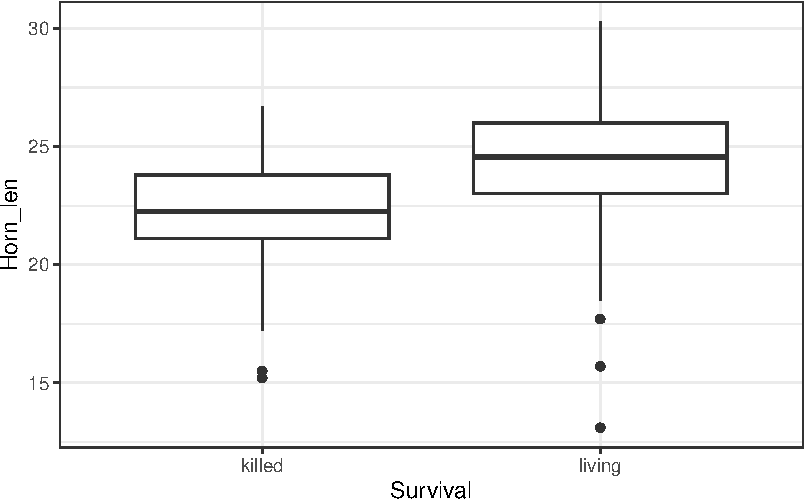
\includegraphics[keepaspectratio]{03-TwoSampleTests_files/figure-pdf/unnamed-chunk-32-1.pdf}}

\subsection{Exercice d'application}\label{exercice-dapplication-1}

Reprenez chaque exemple et exercice traité depuis le premier chapitre et
identifiez les situations où un test unilatéral aurait du sens. Si vous
en trouvez, faites ce test et assurez-vous que les hypothèses choisies
sont bien celles qui sont utilisées lors du test.

\bookmarksetup{startatroot}

\chapter{Structure des populations}\label{structure-des-populations}

\section{Objectifs}\label{objectifs-1}

Ce TP fait le pont direct avec vos cours magistraux. Vous allez y
explorer les deux facettes fondamentales de l'écologie quantitative :

\begin{enumerate}
\def\labelenumi{\arabic{enumi}.}
\tightlist
\item
  \textbf{L'approche du détective (Modèle statistique) :} Comment
  estimer la vraie survie d'une population quand on rate des individus
  sur le terrain (détection imparfaite) ?
\item
  \textbf{L'approche de l'architecte (Modèle de processus) :} Comment
  utiliser ces estimations pour construire un système, simuler l'avenir
  et tester des stratégies de conservation ?
\end{enumerate}

À l'issue de cette séance, vous serez capables de : * Lire et
interpréter un historique de Capture-Marquage-Recapture (CMR). * Ajuster
un modèle simple pour séparer la survie (\(\phi\)) de la probabilité de
détection (\(p\)). * Construire une matrice de Leslie et simuler la
dynamique d'une population structurée en stades (cinétique). * Évaluer
la sensibilité d'une espèce longévive, en lien avec la ``spirale de
l'extinction'' vue en cours.

\section{Avant de vous lancer\ldots{}}\label{avant-de-vous-lancer}

Pour travailler sereinement, créez un nouveau script (nommez-le par
exemple \texttt{TP1\_Systemes\_Dynamiques.R}) à l'intérieur de votre
projet sous Positron.

Bonne nouvelle : \textbf{vous n'aurez aucun fichier externe à
télécharger ou à importer pour ce TP !} Les données sont déjà intégrées
dans les packages R que nous allons utiliser. Vous avez juste besoin de
charger trois bibliothèques (installez-les via la console de Positron si
ce n'est pas encore fait avec
\texttt{install.packages(c("marked",\ "popbio",\ "tidyverse"))}) :

\begin{Shaded}
\begin{Highlighting}[]
\FunctionTok{library}\NormalTok{(tidyverse) }\CommentTok{\# La caisse à outils pour manipuler les données}
\FunctionTok{library}\NormalTok{(marked)    }\CommentTok{\# Pour les modèles de Capture{-}Marquage{-}Recapture (Le Détective)}
\FunctionTok{library}\NormalTok{(popbio)    }\CommentTok{\# Pour les matrices de dynamique des populations (L\textquotesingle{}Architecte)}
\end{Highlighting}
\end{Shaded}

\begin{center}\rule{0.5\linewidth}{0.5pt}\end{center}

\section{Le Détective : Inférence et Probabilité de Détection
(CMR)}\label{le-duxe9tective-infuxe9rence-et-probabilituxe9-de-duxe9tection-cmr}

Sur le terrain, la réalité est cruelle : un animal vivant n'est pas
toujours observé. Comme vu en CM avec la mésange sur le bonnet de
l'ornithologue, la probabilité de détection (\(p\)) est presque toujours
inférieure à 1.

Nous allons utiliser le jeu de données \texttt{dipper} (inclus dans le
package \texttt{marked}). Il s'agit d'un suivi réel du Cincle plongeur
(\emph{Cinclus cinclus}), un petit oiseau aquatique, suivi pendant
plusieurs années.

\begin{figure}[H]

{\centering 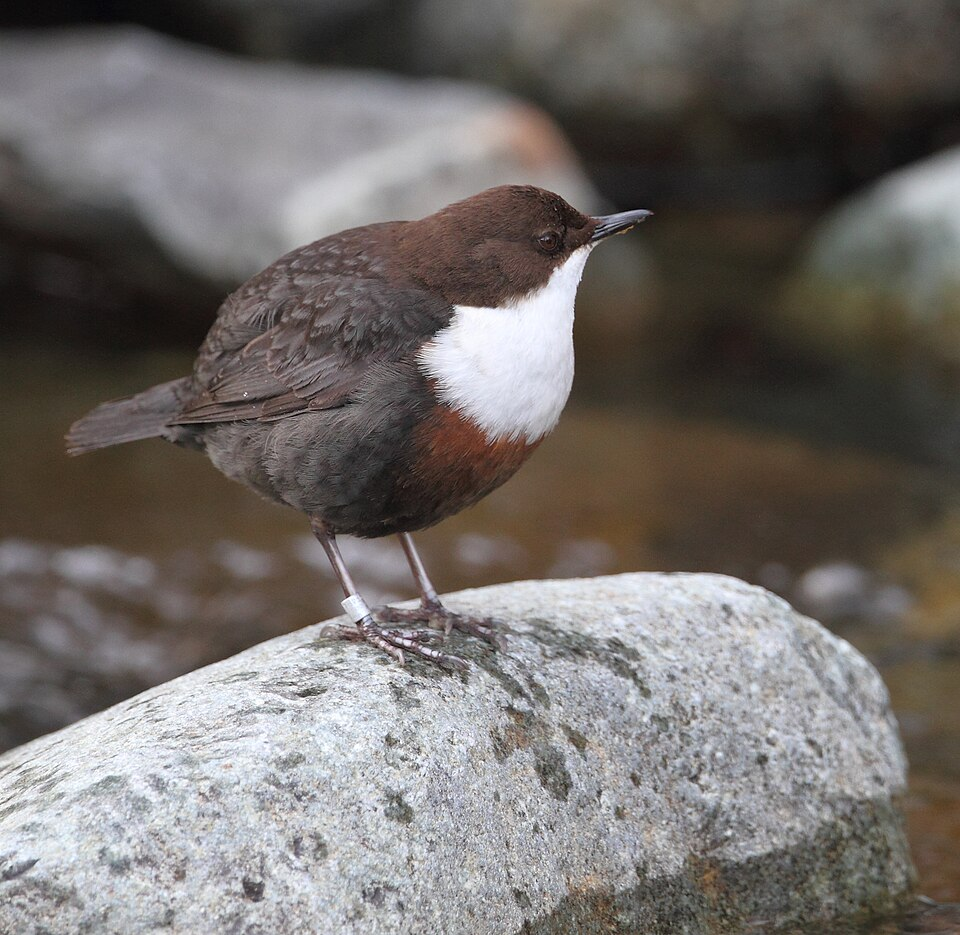
\includegraphics[width=0.5\linewidth,height=\textheight,keepaspectratio]{images/cincle.jpg}

}

\caption{Le Cincle plongeur (\emph{Cinclus cinclus}), inféodé aux cours
d'eau rapides et suivi par baguage (Source : Wikimedia Commons,
CC-BY-SA).}

\end{figure}%

\subsection{Étape 1 : Regarder les données
brutes}\label{uxe9tape-1-regarder-les-donnuxe9es-brutes}

Avant de modéliser, regardons à quoi ressemble un fichier CMR.

\begin{Shaded}
\begin{Highlighting}[]
\CommentTok{\# Chargement et affichage des 6 premières lignes du jeu de données}
\FunctionTok{data}\NormalTok{(dipper)}
\FunctionTok{head}\NormalTok{(dipper)}
\end{Highlighting}
\end{Shaded}

\begin{verbatim}
       ch    sex
1 0000001 Female
2 0000001 Female
3 0000001 Female
4 0000001 Female
5 0000001 Female
6 0000001 Female
\end{verbatim}

\begin{quote}
\textbf{Observation :} Dans la colonne \texttt{ch} (\emph{capture
history}), vous voyez des suites de 0 et de 1 (ex: \texttt{1100000}).

\begin{itemize}
\item
  Un \texttt{1} signifie que l'oiseau a été capturé ou revu cette
  année-là.
\item
  Un \texttt{0} signifie qu'il n'a \textbf{pas} été vu.
\end{itemize}

Si vous voyez un historique comme \texttt{1010000}, cela signifie que
l'oiseau a été vu l'année 1, raté l'année 2, puis revu l'année 3.
\textbf{Puisqu'il a été revu l'année 3, il était obligatoirement vivant
l'année 2 !} Cet historique prouve que l'on rate des individus et
justifie l'utilisation de modèles mathématiques.
\end{quote}

\subsection{Étape 2 : L'ajustement du Modèle de Cormack-Jolly-Seber
(CJS)}\label{uxe9tape-2-lajustement-du-moduxe8le-de-cormack-jolly-seber-cjs}

Nous allons demander à R d'estimer la survie (\(\Phi\)) et la
probabilité de détection (\(p\)). Nous utilisons l'argument
\texttt{formula\ =\ \textasciitilde{}1} pour dire à R : \emph{``Estime
une valeur moyenne constante pour toute la période, sans différencier
les années ou les sexes''}.

\begin{Shaded}
\begin{Highlighting}[]
\CommentTok{\# Ajustement du modèle CJS}
\NormalTok{modele\_cjs }\OtherTok{\textless{}{-}} \FunctionTok{crm}\NormalTok{(dipper, }
                  \AttributeTok{model =} \StringTok{"cjs"}\NormalTok{, }
                  \AttributeTok{model.parameters =} \FunctionTok{list}\NormalTok{(}\AttributeTok{Phi =} \FunctionTok{list}\NormalTok{(}\AttributeTok{formula =} \SpecialCharTok{\textasciitilde{}}\DecValTok{1}\NormalTok{), }
                                          \AttributeTok{p =} \FunctionTok{list}\NormalTok{(}\AttributeTok{formula =} \SpecialCharTok{\textasciitilde{}}\DecValTok{1}\NormalTok{)))}

\CommentTok{\# Affichage des probabilités réelles estimées}
\FunctionTok{predict}\NormalTok{(modele\_cjs)}
\end{Highlighting}
\end{Shaded}

\begin{verbatim}
$Phi
  occ  estimate
1   6 0.5602139

$p
  occ  estimate
1   7 0.9026536
\end{verbatim}

\begin{quote}
\textbf{Point R :} Ne vous laissez pas impressionner par les lignes de
calcul de l'algorithme d'optimisation dans la console de Positron.
Regardez le tableau final produit par \texttt{predict()}. * La
probabilité de survie moyenne d'une année sur l'autre (\(\Phi\)) est
d'environ \textbf{0.56 (56\%)}. * La probabilité de détection (\(p\))
est d'environ \textbf{0.90 (90\%)}. Cela signifie que les chercheurs ont
raté en moyenne 10\% des oiseaux vivants à chaque sortie.
\end{quote}

\begin{center}\rule{0.5\linewidth}{0.5pt}\end{center}

\section{L'Architecte : Le Modèle Matriciel
Structuré}\label{larchitecte-le-moduxe8le-matriciel-structuruxe9}

Le détective a fait son travail. Maintenant, nous changeons d'espèce et
d'échelle pour devenir l'architecte. Pour les populations où la survie
et la reproduction changent avec l'âge, on utilise un \textbf{modèle
structuré} (Matrice de Leslie / Lefkovitch).

Nous allons analyser la population d'Orques (\emph{Orcinus orca}), avec
le jeu de données \texttt{whale} du package \texttt{popbio}.

\begin{figure}[H]

{\centering 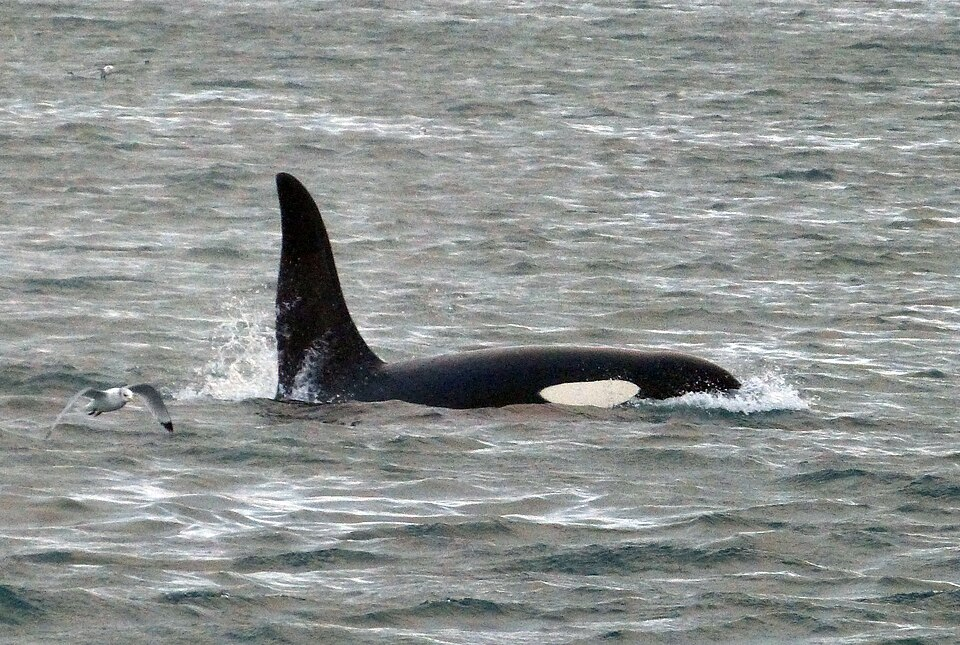
\includegraphics[width=0.65\linewidth,height=\textheight,keepaspectratio]{images/orca.jpg}

}

\caption{Orque mâle adulte (\emph{Orcinus orca}). Reconnaissable à son
imposant aileron dorsal triangulaire pouvant atteindre jusqu'à 2 mètres
de hauteur. Même adultes, les mâles restent généralement fidèles à leur
groupe familial matrilinéaire, guidé par les femelles âgées (Source :
Wikimedia Commons).}

\end{figure}%

\subsection{Étape 1 : Décortiquer la
matrice}\label{uxe9tape-1-duxe9cortiquer-la-matrice}

\begin{Shaded}
\begin{Highlighting}[]
\CommentTok{\# Chargement et affichage de la matrice de l\textquotesingle{}orque}
\FunctionTok{data}\NormalTok{(whale)}
\NormalTok{whale}
\end{Highlighting}
\end{Shaded}

\begin{verbatim}
           yearling juvenile mature postreprod
yearling     0.0000   0.0043 0.1132     0.0000
juvenile     0.9775   0.9111 0.0000     0.0000
mature       0.0000   0.0736 0.9534     0.0000
postreprod   0.0000   0.0000 0.0452     0.9804
\end{verbatim}

\begin{quote}
\textbf{Observation :} Cette matrice carrée \(4 \times 4\) répartit les
individus en 4 stades de développement : \emph{yearling} (1 an),
juvénile, adulte mature, et post-reproductive (ménopause){[}cite: 4{]}.
* Les colonnes représentent le temps \(t\). * Les lignes représentent le
temps \(t+1\). * La \textbf{première ligne} contient la fécondité
(seules les adultes matures se reproduisent, avec un taux de
0.04){[}cite: 4{]}. * Les \textbf{autres lignes} contiennent les
probabilités de survie et de passage d'un stade à l'autre{[}cite: 4{]}.
\end{quote}

\subsection{Étape 2 : Cinétique et Projection
Démographique}\label{uxe9tape-2-cinuxe9tique-et-projection-duxe9mographique}

La cinétique décrit ``comment'' l'abondance varie dans le temps.
Simulons ce qui se passerait sur 50 ans si nous démarrions avec une
toute petite population de 40 orques (10 dans chaque stade).

\begin{Shaded}
\begin{Highlighting}[]
\CommentTok{\# 1. On crée notre vecteur de population de départ}
\NormalTok{n\_initial }\OtherTok{\textless{}{-}} \FunctionTok{c}\NormalTok{(}\DecValTok{10}\NormalTok{, }\DecValTok{10}\NormalTok{, }\DecValTok{10}\NormalTok{, }\DecValTok{10}\NormalTok{)}

\CommentTok{\# 2. On lance la projection mathématique sur 50 ans}
\NormalTok{projection\_orque }\OtherTok{\textless{}{-}} \FunctionTok{pop.projection}\NormalTok{(}\AttributeTok{A =}\NormalTok{ whale, }\AttributeTok{n =}\NormalTok{ n\_initial, }\AttributeTok{iterations =} \DecValTok{50}\NormalTok{)}

\CommentTok{\# 3. On visualise les résultats}
\FunctionTok{stage.vector.plot}\NormalTok{(projection\_orque}\SpecialCharTok{$}\NormalTok{stage.vectors, }
                  \AttributeTok{col =} \DecValTok{1}\SpecialCharTok{:}\DecValTok{4}\NormalTok{, }
                  \AttributeTok{main =} \StringTok{"Dynamique cinétique de la population d\textquotesingle{}Orques"}\NormalTok{)}
\end{Highlighting}
\end{Shaded}

\pandocbounded{
\includegraphics[keepaspectratio]{04-Structure_files/figure-pdf/projection-whale-1.pdf}}

\begin{quote}
\textbf{Observation :} Regardez les 10 premières années sur le
graphique. Les courbes zigzaguent ! C'est ce qu'on appelle
\textbf{l'inertie démographique} vue en CM{[}cite: 6{]}. La population
met du temps à se ``rééquilibrer'' par rapport à notre structure de
départ artificielle. Ensuite, les courbes deviennent parallèles : la
population a atteint sa distribution stable.
\end{quote}

La population va-t-elle s'éteindre ou croître ? Pour le savoir, on
calcule \(\lambda\) (le taux de croissance asymptotique).

\begin{Shaded}
\begin{Highlighting}[]
\FunctionTok{lambda}\NormalTok{(whale)}
\end{Highlighting}
\end{Shaded}

\begin{verbatim}
[1] 1.025441
\end{verbatim}

Si \(\lambda > 1\), la population croît. S'il est \(< 1\), elle décline.
Ici, \(\lambda \approx 1.025\), soit une croissance très lente de 2.5\%
par an, typique des grands mammifères.

\subsection{Étape 3 : Sensibilité et Spirale de
l'Extinction}\label{uxe9tape-3-sensibilituxe9-et-spirale-de-lextinction}

L'orque est une espèce à vie longue (longévive). En cours, nous avons vu
que ces espèces sont extrêmement sensibles à une baisse de la survie des
adultes. Vérifions-le avec la fonction \texttt{sensitivity()}.

\begin{Shaded}
\begin{Highlighting}[]
\CommentTok{\# Calcul de la matrice de sensibilité}
\NormalTok{sensibilite\_orque }\OtherTok{\textless{}{-}} \FunctionTok{sensitivity}\NormalTok{(whale)}

\CommentTok{\# Représentation graphique avec un code couleur}
\FunctionTok{image2}\NormalTok{(sensibilite\_orque, }\AttributeTok{mar =} \FunctionTok{c}\NormalTok{(}\DecValTok{1}\NormalTok{, }\FloatTok{3.5}\NormalTok{, }\DecValTok{5}\NormalTok{, }\DecValTok{1}\NormalTok{), }\AttributeTok{box.offset =} \FloatTok{0.1}\NormalTok{)}
\FunctionTok{title}\NormalTok{(}\StringTok{"Quels paramètres influencent le plus la croissance ?"}\NormalTok{, }\AttributeTok{line =} \FloatTok{2.5}\NormalTok{)}
\end{Highlighting}
\end{Shaded}

\pandocbounded{
\includegraphics[keepaspectratio]{04-Structure_files/figure-pdf/sens-whale-1.pdf}}

\begin{quote}
\textbf{Observation :} Le carré le plus rouge (la plus forte
sensibilité) se situe à l'intersection de la colonne \texttt{mature} et
de la ligne \texttt{mature}. Cela confirme mathématiquement que la
survie des adultes est le pilier de cette population. Une surmortalité
adulte (pollution, braconnage) entraînera une spirale de l'extinction.
\end{quote}

\begin{center}\rule{0.5\linewidth}{0.5pt}\end{center}

\section{À vous de jouer ! (Exercice
autonome)}\label{uxe0-vous-de-jouer-exercice-autonome}

Vous maîtrisez désormais les outils de base. Vous allez les appliquer
sur une espèce terrestre très étudiée en biologie de la conservation :
\textbf{la Tortue du désert} (\emph{Gopherus agassizii}).

\begin{figure}[H]

{\centering 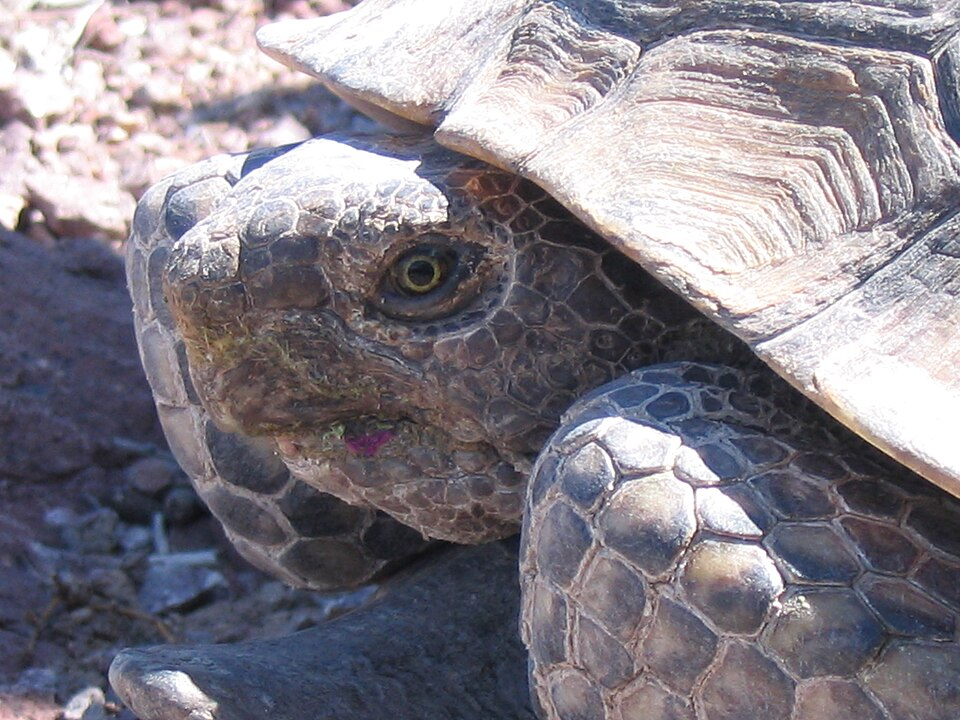
\includegraphics[width=0.55\linewidth,height=\textheight,keepaspectratio]{images/tortoise.jpg}

}

\caption{Tortue du désert (\emph{Gopherus agassizii}), une espèce
menacée dont la viabilité dépend fortement des taux de survie adulte
(Source : Wikimedia Commons, CC-BY).}

\end{figure}%

Le jeu de données \texttt{tortoise} (déjà dans le package
\texttt{popbio}) est une ``liste''. Elle contient 4 matrices de
projection différentes, correspondant à 4 scénarios de fécondité :
basse, moyenne-basse, moyenne-haute, et haute.

\textbf{Votre mission :} Exécutez le code ci-dessous étape par étape
dans Positron et répondez aux questions sur votre brouillon.

\textbf{1. Découverte des données}

\begin{Shaded}
\begin{Highlighting}[]
\FunctionTok{data}\NormalTok{(tortoise)}
\CommentTok{\# Affichons seulement la matrice du scénario "moyenne{-}haute" (med.high)}
\NormalTok{tortoise[[}\StringTok{"med.high"}\NormalTok{]]}
\end{Highlighting}
\end{Shaded}

\begin{verbatim}
         yearling  juv1  juv2  imm1  imm2 subadult adult1 adult2
yearling    0.000 0.000 0.000 0.000 0.000    1.300  1.980   2.57
juv1        0.716 0.567 0.000 0.000 0.000    0.000  0.000   0.00
juv2        0.000 0.149 0.567 0.000 0.000    0.000  0.000   0.00
imm1        0.000 0.000 0.149 0.604 0.000    0.000  0.000   0.00
imm2        0.000 0.000 0.000 0.235 0.560    0.000  0.000   0.00
subadult    0.000 0.000 0.000 0.000 0.225    0.678  0.000   0.00
adult1      0.000 0.000 0.000 0.000 0.000    0.249  0.851   0.00
adult2      0.000 0.000 0.000 0.000 0.000    0.000  0.016   0.86
\end{verbatim}

\textbf{2. Viabilité de la population} Calculez le taux de croissance
(\(\lambda\)) du scénario \texttt{med.high}. \emph{Question : Cette
population est-elle en croissance ou en déclin ?}

\begin{Shaded}
\begin{Highlighting}[]
\FunctionTok{lambda}\NormalTok{(tortoise[[}\StringTok{"med.high"}\NormalTok{]])}
\end{Highlighting}
\end{Shaded}

\textbf{3. Comparaison des scénarios} La fonction \texttt{sapply()}
permet d'appliquer la fonction \texttt{lambda} aux 4 matrices d'un seul
coup. C'est magique !

\begin{Shaded}
\begin{Highlighting}[]
\FunctionTok{sapply}\NormalTok{(tortoise, lambda)}
\end{Highlighting}
\end{Shaded}

\emph{Question : Quel est le seul scénario (parmi les 4) qui provoque un
déclin démographique (la spirale de l'extinction) ?}

\textbf{4. Quelle action de conservation privilégier ?} Générez le
graphique de sensibilité pour la population avec une ``haute''
fécondité.

\begin{Shaded}
\begin{Highlighting}[]
\CommentTok{\# Astuce : remplacez "???" par le nom de la matrice "haute" (regardez le résultat de la question 3 pour trouver son nom exact)}
\NormalTok{sens\_tortue }\OtherTok{\textless{}{-}} \FunctionTok{sensitivity}\NormalTok{(tortoise[[}\StringTok{"???"}\NormalTok{]])}
\FunctionTok{image2}\NormalTok{(sens\_tortue, }\AttributeTok{mar =} \FunctionTok{c}\NormalTok{(}\DecValTok{1}\NormalTok{, }\FloatTok{3.5}\NormalTok{, }\DecValTok{5}\NormalTok{, }\DecValTok{1}\NormalTok{), }\AttributeTok{box.offset =} \FloatTok{0.1}\NormalTok{)}
\end{Highlighting}
\end{Shaded}

\emph{Question : Sur la base de ce graphique (le carré le plus rouge),
si vous étiez gestionnaire de réserve, concentreriez-vous votre budget
pour protéger les nids (fécondité, ligne 1) ou pour empêcher la
mortalité des adultes reproducteurs ? Le constat est-il le même que pour
l'Orque ?}

\bookmarksetup{startatroot}

\chapter{Analyse de cohortes}\label{sec-cohortes}

\section{Objectifs}\label{objectifs-2}

Cette section doit permettre d'illustrer la partie du cours de
Population Dynamics de l'EC ``Fonctionnement des écosystèmes'' consacrée
à l'analyse des cohortes. Vous utiliserez les tailles corporelles
d'individus échantillonnés sur le terrain à plusieurs dates pour :

\begin{enumerate}
\def\labelenumi{\arabic{enumi}.}
\tightlist
\item
  Produire la structure démographique instantanée de la population pour
  chaque date d'échantillonnage
\item
  Réaliser la décomposition polymodale pour identifier les cohortes à
  chaque date d'échantillonnage
\item
  Créer une courbe de croissance et une courbe de mortalité
\item
  Utiliser une relation allométrique pour passer de la taille des
  individus à leur masse
\item
  Produire la courbe d'Allen
\end{enumerate}

Vous devrez en premier lieu importer les données fournies dans un
fichier Excel et vous assurer qu'elles sont dans un format permettant
les analyses et représentations graphiques.

\section{Présentation de l'étude}\label{sec-pres}

Le suivi démographique des populations animales est extrêmement fréquent
dans le domaine de l'écologie. Le suivi des populations naturelles est
particulièrement pertinent dans un contexte de conservation, pour
réaliser des études d'impact ou pour mesurer l'évolution de la
biodiversité.

Ici, une population de gastéropodes \emph{Nassarius reticulatus} (la
nasse réticulée) a été suivie pendant 5 ans. Deux sessions
d'échantillonnage ont été organisées chaque année depuis 2010 : la
première a été réalisée en mars, juste après le recrutement des
juvéniles, et la seconde a été réalisée 6 mois plus tard, en septembre.
Tous les échantillons ont été collectés au même endroit, selon la même
méthode (collecte systématique de tous les individus présents à
l'intérieur de 10 quadrats positionnés aléatoirement dans la zone
d'étude), lors d'une marée basse de fort coefficient (marées de
printemps et d'automne). Les individus échantillonnés ont été mesurés
sur place, de la base, à l'apex de la coquille (voir
Figure~\ref{fig-nasse}) à l'aide d'un pied à coulisse (précision :
centième de millimètre) et relâchés sur place.

\begin{marginfigure}

\centering{

\pandocbounded{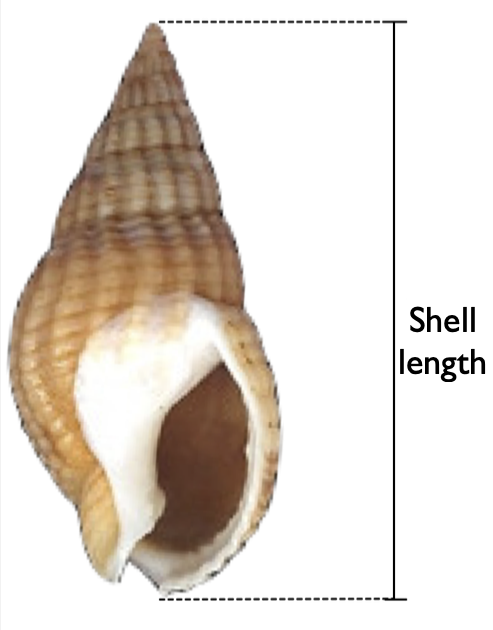
\includegraphics[keepaspectratio]{images/Nassarius.png}}

}

\caption{\label{fig-nasse}Coquille de nasse réticulée \emph{Nassarius
reticulatus} (Linnaeus, 1758)}

\end{marginfigure}%

L'espèce étudiée présente les caractéristiques suivantes :

\begin{itemize}
\tightlist
\item
  Les individus ont une durée de vie de 5 ans en moyenne.
\item
  Les plus grands individus peuvent atteindre une taille de plus de 40
  millimètres.
\item
  Il n'y a qu'une seule période de reproduction chaque année. Il n'y a
  donc qu'un unique recrutement chaque année, au tout début du mois de
  mars.
\end{itemize}

Des travaux antérieurs, réalisés au laboratoire, ont montré que la
taille et la masse des individus étaient liées par la relation
allométrique suivante :

\[w = 0,0013 \cdot l^{2,3}\]

avec \(w\), la masse en grammes et \(l\) la longueur des coquilles en
millimètres.

\begin{tcolorbox}[enhanced jigsaw, arc=.35mm, bottomrule=.15mm, bottomtitle=1mm, breakable, colback=white, colbacktitle=quarto-callout-important-color!10!white, colframe=quarto-callout-important-color-frame, coltitle=black, left=2mm, leftrule=.75mm, opacityback=0, opacitybacktitle=0.6, rightrule=.15mm, title=\textcolor{quarto-callout-important-color}{\faExclamation}\hspace{0.5em}{Objectif principal}, titlerule=0mm, toprule=.15mm, toptitle=1mm]

L'objectif principal de cette étude est de produire la courbe d'Allen
d'une cohorte de cette populations. Cette courbe sera utilisée pour
déterminer des gains et des pertes de biomasses au sein de l'écosystème
étudié. Les étapes nécessaires à la production de cette courbe sont
présentées ci-dessous.

\end{tcolorbox}

\section{Avant de vous lancer\ldots{}}\label{avant-de-vous-lancer-1}

Pour travailler dans de bonnes conditions, vous aurez absolument besoin
de travailler dans un script et à l'intérieur d'un \texttt{Rproject}. Si
vous ne savez plus comment faire, reportez-vous aux chapitres
correspondants du livre en ligne de Biométrie du semestre 3 :
\href{https://besibo.github.io/BiometrieS3/01-R-basics.html\#sec-script}{au
sujet des scripts} et
\href{https://besibo.github.io/BiometrieS3/01-R-basics.html\#les-projets-ou-rprojects}{au
sujet des \texttt{Rprojects}}. Vous devrez notamment (liste non
exhaustive !) :

\begin{enumerate}
\def\labelenumi{\arabic{enumi}.}
\tightlist
\item
  Créer un nouveau script (nommez-le \texttt{Nasses.R})
\item
  Télécharger (si besoin) et charger quelques packages (voir plus bas)
\item
  Télécharger dans votre répertoire de travail le fichier Nassarius.csv
\item
  Importer dans \texttt{RStudio} les données du fichier
  \texttt{Nassarius.csv}
\end{enumerate}

Pour cette section, vous aurez besoin des packages suivants :

\begin{itemize}
\tightlist
\item
  \texttt{tidyverse} : pour manipuler les données et faire des
  graphiques (Wickham et al. 2019)
\item
  \texttt{mixdist} : pour effectuer les décompositions polymodales
  (Macdonald et Juan Du 2018)
\end{itemize}

Si vous ne savez plus comment installer et charger des packages en
mémoire, reportez-vous au chapitre correspondant du
\href{https://besibo.github.io/BiometrieS3/01-R-basics.html\#sec-packages}{livre
en ligne de Biométrie du semestre 3}

\begin{Shaded}
\begin{Highlighting}[]
\FunctionTok{library}\NormalTok{(tidyverse)}
\FunctionTok{library}\NormalTok{(mixdist)}
\end{Highlighting}
\end{Shaded}

Pour importer les données, utilisez l'assistant d'importation de
\texttt{RStudio}. Notez que :

\begin{itemize}
\tightlist
\item
  Les colonnes sont séparées par des tabulations
\item
  Le symbole utilisé pour les décimales dans le fichier
  \texttt{Nassarius.csv} est la virgule
\end{itemize}

Vous devrez donc spécifier correctement ces éléments pour pouvoir
importer le fichier dans le logiciel. Si vous ne savez plus comment
faire, reportez-vous au chapitre correspondant du
\href{https://besibo.github.io/BiometrieS3/04-DataWrangling.html\#plaintext}{livre
en ligne de Biométrie du semestre 3}.

Si l'importation s'est déroulée normalement, vous devriez maintenant
disposer de l'objet nommé \texttt{Nassarius} suivant :

\begin{Shaded}
\begin{Highlighting}[]
\NormalTok{Nassarius}
\end{Highlighting}
\end{Shaded}

\begin{verbatim}
# A tibble: 3,710 x 2
    size date    
   <dbl> <chr>   
 1  4.8  march-10
 2  3    march-10
 3  5.56 march-10
 4  3.74 march-10
 5  4.1  march-10
 6  2.21 march-10
 7  2.75 march-10
 8  3.18 march-10
 9  2.56 march-10
10  4.36 march-10
# i 3,700 more rows
\end{verbatim}

Et la commande suivante devrait produire exactement ces résultats :

\begin{Shaded}
\begin{Highlighting}[]
\NormalTok{Nassarius }\SpecialCharTok{|\textgreater{}}
  \FunctionTok{count}\NormalTok{(date)}
\end{Highlighting}
\end{Shaded}

\begin{verbatim}
# A tibble: 10 x 2
   date         n
   <chr>    <int>
 1 march-10   468
 2 march-11   481
 3 march-12   460
 4 march-13   468
 5 march-14   487
 6 sept-10    268
 7 sept-11    276
 8 sept-12    265
 9 sept-13    258
10 sept-14    279
\end{verbatim}

\marginnote{\begin{footnotesize}

\texttt{\textbar{}\textgreater{}} : le pipe est un opérateur spécial qui
prend l'objet situé à gauche et le transmets à la fonction placée à
droite, en guise de premier argument. P. ex. :
\texttt{Nassarius\ \textbar{}\textgreater{}\ count(date)} est équivalent
à \texttt{count(Nassarius,\ date)}\\
\texttt{count()} : compte le nombre d'occurrences de chaque valeur
possible (ou niveau/modalité) d'une variable catégorielle (ou facteur).

\end{footnotesize}}

\section{Les étapes de l'analyse}\label{les-uxe9tapes-de-lanalyse}

Pour produire une courbe d'Allen, de nombreuses étapes sont nécessaires.
Vous devrez :

\begin{enumerate}
\def\labelenumi{\arabic{enumi}.}
\tightlist
\item
  Produire la \emph{structure démographique instantanée} de la
  population à chaque date d'échantillonnage
\item
  Réaliser la \emph{décomposition polymodale} pour identifier les
  cohortes présentes dans la population à chaque date d'échantillonnage.
\item
  Déterminer la taille moyenne de la coquille des individus de la
  cohorte d'intérêt, à chaque date d'échantillonnage, pour produire la
  \emph{courbe de croissance}
\item
  Déterminer l'abondance des individus de la cohorte d'intérêt, à chaque
  date d'échantillonnage, pour produire la \emph{courbe de survie}
\end{enumerate}

Je vais présenter ci-dessous les étapes de cette procédure \textbf{pour
une unique date d'échantillonnage} : march 2010. Vous devrez reproduire
ces étapes pour les 9 autres dates d'échantillonnage.

\section{Sélection des données d'une date
spécifique}\label{suxe9lection-des-donnuxe9es-dune-date-spuxe9cifique}

Notre jeu de données \texttt{Nassrisu} contient 2 colonnes : la première
contient les dates d'échantillonnage et la seconde les tailles
individuelles en millimètres. La première étape consiste à créer un
nouvel objet (nous le nommerons \texttt{Nas\_01}) qui contiendra
uniquement les données collectées lors de la toute première session
d'échantillonnage de mars 2010. Vous devriez déjà savoir comment
utiliser la fonction \texttt{filter()} pour le faire :

\begin{Shaded}
\begin{Highlighting}[]
\NormalTok{Nas\_01 }\OtherTok{\textless{}{-}}\NormalTok{ Nassarius }\SpecialCharTok{|\textgreater{}}
  \FunctionTok{filter}\NormalTok{(date }\SpecialCharTok{==} \StringTok{"march{-}10"}\NormalTok{)}

\NormalTok{Nas\_01}
\end{Highlighting}
\end{Shaded}

\begin{verbatim}
# A tibble: 468 x 2
    size date    
   <dbl> <chr>   
 1  4.8  march-10
 2  3    march-10
 3  5.56 march-10
 4  3.74 march-10
 5  4.1  march-10
 6  2.21 march-10
 7  2.75 march-10
 8  3.18 march-10
 9  2.56 march-10
10  4.36 march-10
# i 458 more rows
\end{verbatim}

\marginnote{\begin{footnotesize}

\texttt{filter()} : permet de filtrer les lignes d'un tableau (ici
\texttt{Nassarius}) pour ne conserver que celles qui remplissent une
condition spécifiée par l'utilisateur (ici
\texttt{date\ ==\ "march\_10"})

\end{footnotesize}}

\begin{Shaded}
\begin{Highlighting}[]
\FunctionTok{dim}\NormalTok{(Nassarius)}
\end{Highlighting}
\end{Shaded}

\begin{verbatim}
[1] 3710    2
\end{verbatim}

\begin{Shaded}
\begin{Highlighting}[]
\FunctionTok{dim}\NormalTok{(Nas\_01)}
\end{Highlighting}
\end{Shaded}

\begin{verbatim}
[1] 468   2
\end{verbatim}

\marginnote{\begin{footnotesize}

\texttt{dim()} : Affiche le nombre de lignes et de colonnes d'un
tableau.

\end{footnotesize}}

Comme nous pouvons le constater, on passe du tableau original
\texttt{Nasarius} contenant 3710 lignes à un nouveau tableau
\texttt{Nas\_01} qui en contient seulement 468.

\section{Structure démographique
instantanée}\label{structure-duxe9mographique-instantanuxe9e}

Maintenant que nous disposons d'une table \texttt{Nas\_01} qui contient
uniquement la taille des individus collectés en mars 2010, il nous faut
visualiser la structure démographique instantanée afin de déterminer
combien de cohortes étaient présentes dans la population à cette date.
La structure démographique instantanée est ici simplement un histogramme
présentant la distribution des tailles individuelles. Nous allons donc
placer la taille des individus sur l'axe des \texttt{x} en guise de
descripteur individuel, et sur l'axe des \texttt{y}, \texttt{RStudio}
placera automatiquement l'abondance pour chaque classe de taille en
guise de descripteur populationnel.

\begin{Shaded}
\begin{Highlighting}[]
\NormalTok{Nas\_01 }\SpecialCharTok{|\textgreater{}}
  \FunctionTok{ggplot}\NormalTok{(}\FunctionTok{aes}\NormalTok{(}\AttributeTok{x =}\NormalTok{ size)) }\SpecialCharTok{+}
  \FunctionTok{geom\_histogram}\NormalTok{()}
\end{Highlighting}
\end{Shaded}

\begin{verbatim}
`stat_bin()` using `bins = 30`. Pick better value with `binwidth`.
\end{verbatim}

{
\makeatletter
\def\LT@makecaption#1#2#3{%
  \noalign{\smash{\hbox{\kern\textwidth\rlap{\kern\marginparsep
  \parbox[t]{\marginparwidth}{%
    \footnotesize{%
      \vspace{(1.1\baselineskip)}
    #1{#2: }\ignorespaces #3}}}}}}%
    }
\makeatother

\begin{figure}[H]

\sidecaption{\label{fig-histo1}Structure démographique instantanée}

\centering{

\pandocbounded{
\includegraphics[keepaspectratio]{05-Cohortes_files/figure-pdf/fig-histo1-1.pdf}}

}

\end{figure}%

}

\marginnote{\begin{footnotesize}

\texttt{ggplot()} : crée un graphique\\
\texttt{aes()} : associe une variable d'un jeu de données à une
caractéristique esthétique d'un graphique (p.~ex. la position le long de
l'axe des \texttt{x} ou des \texttt{y}, la couleur, la forme, la taille,
etc.)\\
\texttt{geom\_histogram()} : ajoute un objet géométrique de type
histogramme à une graphique produit par \texttt{ggplot()}

\end{footnotesize}}

Notez le message d'avertissement qui s'affiche quand vous produisez cet
histogramme. Il indique que \texttt{R} a choisi pour nous le nombre de
classes de tailles. Par défaut, il crée 30 classes, mais nous indique
que ce n'est certainement pas le meilleur choix. Nous allons donc devoir
créer nous même manuellement les classes de tailles pour (i) identifier
les cohortes présentes dans la population et (ii) fixer des classes
identiques que nous utiliserons pour toutes les autres dates
d'échantillonnage et qui rendront les comparaisons plus aisées.

Puisque les individus de cette espèce peuvent atteindre une taille de 40
millimètres environ, nous allons définir des classes de tailles tous les
millimètres. On peut faire ça simplement en créant un vecteur qui
contient les limites des classes de tailles que l'on souhaite :

\begin{Shaded}
\begin{Highlighting}[]
\CommentTok{\# Calcul de la taille maximale observée}
\NormalTok{taille\_max }\OtherTok{\textless{}{-}} \FunctionTok{max}\NormalTok{(Nassarius}\SpecialCharTok{$}\NormalTok{size, }\AttributeTok{na.rm =} \ConstantTok{TRUE}\NormalTok{)}
\NormalTok{taille\_max}
\end{Highlighting}
\end{Shaded}

\begin{verbatim}
[1] 41.33
\end{verbatim}

\marginnote{\begin{footnotesize}

\texttt{max()} : affiche la valeur maximale contenue dans un vecteur

\end{footnotesize}}

\begin{Shaded}
\begin{Highlighting}[]
\CommentTok{\# Définition des limites des classes de tailles}
\NormalTok{limites }\OtherTok{\textless{}{-}} \DecValTok{0}\SpecialCharTok{:}\NormalTok{(taille\_max }\SpecialCharTok{+} \DecValTok{1}\NormalTok{)}
\NormalTok{limites}
\end{Highlighting}
\end{Shaded}

\begin{verbatim}
 [1]  0  1  2  3  4  5  6  7  8  9 10 11 12 13 14 15 16 17 18 19 20 21 22 23 24
[26] 25 26 27 28 29 30 31 32 33 34 35 36 37 38 39 40 41 42
\end{verbatim}

\marginnote{\begin{footnotesize}

\texttt{:} : l'opérateur ``deux points'' permet de créer des suites
d'entiers

\end{footnotesize}}

L'objet \texttt{limites} contient les limites des classes de tailles que
nous utiliserons pour produire les structures démographiques
instantanées, pour chaque date d'échantillonnage, et pas seulement pour
mars 2010. C'est la raison pour nous avons utilisé
\texttt{max(Nassarius\$size)\ +1} : cette syntaxe nous assure que nos
classes de tailles recouvrent bien la taille de tous les individus
échantillonnés au cours des 5 années d'études. Ainsi, nous pourrons
utiliser les mêmes classes de tailles pour toutes les dates.

Maintenant, on peut utiliser le vecteur \texttt{limites} comme argument
de la fonction \texttt{geom\_histogram()}. On modifie aussi les couleurs
des barres de l'histogramme pour mieux visualiser les classes :

\begin{Shaded}
\begin{Highlighting}[]
\NormalTok{Nas\_01 }\SpecialCharTok{|\textgreater{}}
  \FunctionTok{ggplot}\NormalTok{(}\FunctionTok{aes}\NormalTok{(}\AttributeTok{x =}\NormalTok{ size)) }\SpecialCharTok{+}
  \FunctionTok{geom\_histogram}\NormalTok{(}\AttributeTok{breaks =}\NormalTok{ limites, }\AttributeTok{color =} \StringTok{"black"}\NormalTok{, }\AttributeTok{fill =} \StringTok{"steelblue"}\NormalTok{)}
\end{Highlighting}
\end{Shaded}

{
\makeatletter
\def\LT@makecaption#1#2#3{%
  \noalign{\smash{\hbox{\kern\textwidth\rlap{\kern\marginparsep
  \parbox[t]{\marginparwidth}{%
    \footnotesize{%
      \vspace{(1.1\baselineskip)}
    #1{#2: }\ignorespaces #3}}}}}}%
    }
\makeatother

\begin{figure}[H]

\sidecaption{\label{fig-histo2}Structure démographique instantanée
utilisable pour la décomposition polymodale}

\centering{

\pandocbounded{
\includegraphics[keepaspectratio]{05-Cohortes_files/figure-pdf/fig-histo2-1.pdf}}

}

\end{figure}%

}

Cette structure démographique instantanée (Figure~\ref{fig-histo2}) fait
apparaître 5 cohortes, bien que la plus âgée soit à peine visible. Les
pics, ou modes, sont situés autour de 4, 9, 17, 30 et 34 millimètres.
Ces valeurs approximatives sont importantes car nous les utiliserons
pour réaliser la décomposition polymodale.

\section{Décomposition polymodale}\label{duxe9composition-polymodale}

\subsection{Principe et étapes}\label{principe-et-uxe9tapes}

Effectuer une décomposition polymodale revient à tenter d'ajuster une
distribution Normale à chaque cohorte de la population. Puisque nous
avons identifié 5 cohortes dans la population en mars 2010, il nous faut
identifier 5 distribution Normales distinctes dont la somme reproduira
le plus fidèlement possible la structure démographique instantanée
observée. Plusieurs étapes sont requises pour y parvenir.

Nous allons utiliser le package \texttt{mixdist}, que vous devez avoir
déjà installé et chargé en mémoire. Ce package fournit plusieurs
fonctions relativement simples d'utilisation et qui permettent d'ajuster
des distributions Normales à une distribution observée (notre structure
démographique instantanée).

La fonction du package \texttt{mixdist} qui nous permettra de réaliser
la décomposition polymodale est la fonction \texttt{mix()}. Son fichier
d'aide nous indique que pour fonctionner correctement, il faut lui
fournir plusieurs choses :

\begin{Shaded}
\begin{Highlighting}[]
\NormalTok{?}\FunctionTok{mix}\NormalTok{()}
\end{Highlighting}
\end{Shaded}

\marginnote{\begin{footnotesize}

\texttt{?} : l'opérateur ``point d'interrogation'' suivi du nom d'une
fonction, permet d'ouvrir le fichier d'aide de cette fonction.

\end{footnotesize}}

Les deux premiers arguments de la fonction \texttt{mix()} ne possèdent
pas de valeur par défaut. Nous devons donc spécifier nous même ces deux
arguments :

\begin{enumerate}
\def\labelenumi{\arabic{enumi}.}
\tightlist
\item
  Le premier s'appelle \texttt{mixdat}. Il doit obligatoirement s'agir
  d'un tableau de données (\texttt{data.frame} ou \texttt{tibble})
  contenant 2 colonnes. La première colonne doit contenir les limites
  supérieures des classes de tailles de notre structure démographique
  instantanée. Le dernier élément de cette colonne doit être ``ouvert''
  : il doit être fixé à \(+\infty\). La seconde colonne doit contenir
  les abondances pour chaque classe de taille de la structure
  démographique instantanée. Nous allons voir juste après comment créer
  cet objet \texttt{mixdat}.
\item
  Le second argument s'appelle \texttt{mixpar}. Là encore, il s'agit
  d'un tableau de données. Il doit contenir des valeurs approchées pour
  les paramètres des distributions Normales que nous souhaitons ajuster
  à chacune de nos 5 cohortes. Chaque distribution Normale possède 2
  paramètres : la moyenne (qui correspond à la position du pic sur l'axe
  des \texttt{x} d'un histogramme) et l'écart-type (qui correspond à
  l'étalement de la courbe en cloche, c'est-à-dire à la dispersion des
  données de part et d'autre de la moyenne). Là encore, nous verrons
  plus bas comment créer cet objet.
\end{enumerate}

\subsection{Création du premier
objet}\label{cruxe9ation-du-premier-objet}

Pour créer le premier tableau qui sera utilisé comme argument
\texttt{mixdat} de la fonction \texttt{mix()}, nous allons nous servir
de la fonction \texttt{mixgroup()} du package \texttt{mixdist}. Elle est
très simple `a utiliser puisqu'elle n'a besoin que de 2 arguments :

\begin{enumerate}
\def\labelenumi{\arabic{enumi}.}
\tightlist
\item
  Un vecteur de données (ici, la taille de tous les individus
  échantillonnés en mars 2010)
\item
  La liste des valeurs correspondant aux limites des classes de tailles
  de la structure démographique instantanée. Nous disposons déjà de cet
  objet puisque nous l'avons créé plus tôt : c'est le vecteur
  \texttt{limites}
\end{enumerate}

\begin{Shaded}
\begin{Highlighting}[]
\NormalTok{mix\_01 }\OtherTok{\textless{}{-}} \FunctionTok{mixgroup}\NormalTok{(Nas\_01}\SpecialCharTok{$}\NormalTok{size, }\AttributeTok{breaks =}\NormalTok{ limites)}
\FunctionTok{class}\NormalTok{(mix\_01)}
\end{Highlighting}
\end{Shaded}

\begin{verbatim}
[1] "mixdata"    "data.frame"
\end{verbatim}

L'objet \texttt{mix\_01} que nous venons de créer est donc un
\texttt{data.frame}, mais c'est aussi un objet de classe
\texttt{mixdata} que nous utiliserons en guise de premier argument de la
fonction \texttt{mix()}. Pour afficher son contenu, il suffit comme
toujours de taper son nom :

\begin{Shaded}
\begin{Highlighting}[]
\NormalTok{mix\_01}
\end{Highlighting}
\end{Shaded}

\begin{verbatim}
     X count
1    1     1
2    2     6
3    3    39
4    4    70
5    5    69
6    6    30
7    7    19
8    8    23
9    9    26
10  10    33
11  11    19
12  12     7
13  13     2
14  14     1
15  15     4
16  16     5
17  17    10
18  18    15
19  19     7
20  20    13
21  21     6
22  22     5
23  23     2
24  24     1
25  25     4
26  26     4
27  27     6
28  28     2
29  29     7
30  30     8
31  31     3
32  32     4
33  33     3
34  34     4
35  35     3
36  36     1
37  37     2
38  38     2
39  39     2
40  40     0
41  41     0
42 Inf     0
\end{verbatim}

Notez que la dernière ligne de \texttt{mix\_01} correspond à la
catégorie {[}42 mm ; \(+\infty\){[}. Pour vérifier que nous n'avons pas
fait d'erreur, on peut faire une représentation graphique de cet objet
particulier avec la fonction \texttt{plot()} :

\begin{Shaded}
\begin{Highlighting}[]
\FunctionTok{plot}\NormalTok{(mix\_01, }\AttributeTok{xlab =} \StringTok{"Size (mm)"}\NormalTok{, }\AttributeTok{ylab =} \StringTok{"Probability"}\NormalTok{)}
\end{Highlighting}
\end{Shaded}

{
\makeatletter
\def\LT@makecaption#1#2#3{%
  \noalign{\smash{\hbox{\kern\textwidth\rlap{\kern\marginparsep
  \parbox[t]{\marginparwidth}{%
    \footnotesize{%
      \vspace{(1.1\baselineskip)}
    #1{#2: }\ignorespaces #3}}}}}}%
    }
\makeatother

\begin{figure}

\sidecaption{\label{fig-mixplot}Le contenu de \texttt{mix\_01}
correspond exactement à la structure démographique instantanée de mars
2010. La ligne bleue est le contour de la structure démographique
instantanée, qui devra être approchée par la superposition de 5 courbes
Normales correspondant au 5 cohortes qui composent la population en mars
2010}

\centering{

\pandocbounded{
\includegraphics[keepaspectratio]{05-Cohortes_files/figure-pdf/fig-mixplot-1.pdf}}

}

\end{figure}%

}

\marginnote{\begin{footnotesize}

\texttt{plot()} : fonction générique permettant de produire des
graphiques sans \texttt{ggplot2}. La forme du résultat dépendra de la
classe de l'objet utilisé comme argument.

\end{footnotesize}}

Au final, l'objet \texttt{mix\_01} est simplement la structure
démographique instantanée de mars 2010, présentée dans un format qui
sera compris par la fonction \texttt{mix()} que nous utiliserons pour
effectuer la décomposition polymodale.

\subsection{Création du deuxième
objet}\label{cruxe9ation-du-deuxiuxe8me-objet}

Pour créer le second \texttt{data.frame()} dont la fonction
\texttt{mix()} aura besoin, nous allons utiliser une autre fonction du
package \texttt{mixdist} : la fonction \texttt{mixparam()}. Cette
fonction prend au minimum 2 arguments :

\begin{enumerate}
\def\labelenumi{\arabic{enumi}.}
\tightlist
\item
  \texttt{mu} : un vecteur qui contient la position approximative des
  modes (ou pics) de chaque cohorte. Si nous avons 5 cohortes à
  identifier, il faudra fournir 5 valeurs pour \texttt{mu}. Pour mars
  2010, nous utiliserons les valeurs présentées plus au, au niveau de la
  Figure~\ref{fig-histo2} (4, 9, 17, 30 et 34 millimètres). Ces valeurs
  changeront pour chaque date d'échantillonnage et il faudra donc
  examiner attentivement les structures démographiques instantanées de
  chaque échantillonnage pour les déterminer. J'insiste sur le fait que
  la position des pics peut être approximative, mais qu'elle ne doit
  malgré tout pas être trop éloignée des vraies valeurs.
\item
  \texttt{sigma} : un vecteur qui contient la valeur approchée de
  l'écart-type de chaque cohorte. L'écart-type d'une cohorte correspond
  à l'étalement des tailles de part et d'autres de la moyenne de la
  cohorte. C'est ce que nous avons appelé ``polymorphisme'' dans le
  cours de dynamique des populations, puisque cet étalement représente
  des performances de croissance variables pour des individus qui sont
  tous nés approximativement en même temps. Là encore, il faut fournir
  autant de valeurs que nous avons de cohortes (soit 5 pour mars 2010).
  Puisque nous n'avons pas d'idée précise d'ordre de grandeur pour ces
  écarts-types, nous utiliserons la valeur \texttt{1} pour chaque
  cohorte.
\end{enumerate}

Ainsi, on obtient le second \texttt{data.frame} ainsi :

\begin{Shaded}
\begin{Highlighting}[]
\NormalTok{param\_01 }\OtherTok{\textless{}{-}} \FunctionTok{mixparam}\NormalTok{(}\AttributeTok{mu =} \FunctionTok{c}\NormalTok{(}\DecValTok{4}\NormalTok{, }\DecValTok{9}\NormalTok{, }\DecValTok{17}\NormalTok{, }\DecValTok{30}\NormalTok{, }\DecValTok{34}\NormalTok{),}
                     \AttributeTok{sigma =} \FunctionTok{c}\NormalTok{(}\DecValTok{1}\NormalTok{, }\DecValTok{1}\NormalTok{, }\DecValTok{1}\NormalTok{, }\DecValTok{1}\NormalTok{, }\DecValTok{1}\NormalTok{))}
\NormalTok{param\_01}
\end{Highlighting}
\end{Shaded}

\begin{verbatim}
   pi mu sigma
1 0.2  4     1
2 0.2  9     1
3 0.2 17     1
4 0.2 30     1
5 0.2 34     1
\end{verbatim}

\marginnote{\begin{footnotesize}

\texttt{mixparam()} : fonction qui crée un \texttt{data.frame} dans
lequel chaque ligne contient les caractéristiques approchées d'une
cohorte de la population échantillonnée\\
\texttt{c()} : fonction qui permet de créer un vecteur, donc une
collection d'éléments qui sont tous du même type (ici, des valeurs
numériques).

\end{footnotesize}}

La première colonne de ce nouveau \texttt{data.frame}, nommée
\texttt{pi}, correspond à la proportion de l'effectif total
échantillonné, contenu dans chaque cohorte. Puisque nous n'avons rien
spécifié, \texttt{mixparam()} suppose que chaque cohorte contient une
proportion identiques des individus de la population, et fixe donc la
proportion à 0.2 (soit 20\% de l'abondance totale dans chacune des 5
cohortes supposées). Nous savons pertinemment que ces proportions sont
fausses puisqu'en réalité, l'abondance au sein des cohortes décroit avec
l'âge des individus en raison de la mortalité. On sait donc que la
cohorte la plus jeune sera la plus abondante, et que les cohortes plus
âgées seront de moins en moins abondantes. Ces proportions seront
estimées automatiquement par la fonction \texttt{mix()} lorsque nous
réaliserons la décomposition polymodale. Les autres colonnes de
\texttt{param\_01}, qui contiennent les valeurs que nous avons fournies
manuellement, seront également ajustées lors de la décomposition
polymodale

\subsection{Ajustement des lois Normales aux
données}\label{ajustement-des-lois-normales-aux-donnuxe9es}

Maintenant que nous disposons des deux objets nécessaires, nous pouvons
réaliser la décomposition polymodale qui consiste, grâce à la fonction
\texttt{mix()}, à ajuster une distribution Normale à chaque cohorte
supposée de la population échantillonnés.

\begin{Shaded}
\begin{Highlighting}[]
\NormalTok{res\_01 }\OtherTok{\textless{}{-}} \FunctionTok{mix}\NormalTok{(mix\_01, param\_01)}
\end{Highlighting}
\end{Shaded}

\begin{verbatim}
Warning in mix(mix_01, param_01): The optimization process terminated because
iteration limit exceeded
\end{verbatim}

\begin{Shaded}
\begin{Highlighting}[]
\NormalTok{res\_01}
\end{Highlighting}
\end{Shaded}

\begin{verbatim}

Parameters:
       pi     mu sigma
1 0.46418  3.903 1.086
2 0.27062  8.795 1.555
3 0.14355 18.115 2.102
4 0.09100 28.231 2.861
5 0.03066 35.021 2.344

Distribution:
[1] "norm"

Constraints:
   conpi    conmu consigma 
  "NONE"   "NONE"   "NONE" 
\end{verbatim}

\marginnote{\begin{footnotesize}

\texttt{mix()} : réalise la décomposition polymodale. La fonction
identifie une combinaison de distributions Normales qui s'ajuste le
mieux possible aux données observées compte tenu des données brutes et
des caractéristiques approximatives de chaque distribution Normale
fournie par l'utilisateur.

\end{footnotesize}}

La fonction \texttt{mix()} peut produire quelques avertissements.
Ignorez-les à ce stade : seuls les messages d'erreurs sont
problématiques et nous y reviendrons plus tard. L'objet \texttt{res\_01}
contient donc les résultats de la décomposition polymodale. C'est une
liste de 3 éléments dont seul le premier nous intéresse.\^{}{[}Il
s'appelle \texttt{parameters}, sans majuscule, même si \texttt{R}
affiche son nom avec une majuscule. Vous pouvez le vérifier en tapant
\texttt{str(res\_01)}.

\texttt{str()} : affiche la \textbf{str}ucture interne d'objets
complexes.{]} Il contient les valeurs ajustées pour les 3 paramètres des
distributions Normales (\texttt{pi}, \texttt{mu} et \texttt{sigma}) pour
chacune des 5 cohortes identifiées en mars 2010.

Ainsi, par exemple, pour l'échantillon de mars 2010, la première ligne
du tableau \texttt{parameters} contenu dans \texttt{res\_01} nous
apprend les choses suivantes :

\begin{Shaded}
\begin{Highlighting}[]
\NormalTok{res\_01}\SpecialCharTok{$}\NormalTok{parameters}
\end{Highlighting}
\end{Shaded}

\begin{verbatim}
          pi        mu    sigma
1 0.46417552  3.903201 1.085990
2 0.27061610  8.795297 1.555004
3 0.14354832 18.114948 2.101807
4 0.09099874 28.230516 2.861214
5 0.03066132 35.020985 2.343520
\end{verbatim}

\begin{itemize}
\tightlist
\item
  La première cohorte représente 46.42\% de l'abondance totale de la
  population
\item
  La taille moyenne des individus composant cette cohorte vaut 3.9
  millimètres
\item
  L'écart-type (ou polymorphisme de taille) de cette cohorte vaut 1.1
  millimètres
\end{itemize}

Les distributions Normales qui ont été ajustées peuvent être visualisées
grâce à la fonction \texttt{plot()} :

\begin{Shaded}
\begin{Highlighting}[]
\FunctionTok{plot}\NormalTok{(res\_01)}
\end{Highlighting}
\end{Shaded}

{
\makeatletter
\def\LT@makecaption#1#2#3{%
  \noalign{\smash{\hbox{\kern\textwidth\rlap{\kern\marginparsep
  \parbox[t]{\marginparwidth}{%
    \footnotesize{%
      \vspace{(1.1\baselineskip)}
    #1{#2: }\ignorespaces #3}}}}}}%
    }
\makeatother

\begin{figure}

\sidecaption{\label{fig-ajustement}Distribution observée (histogramme
bleu) et cohortes ajustées (courbes rouges). Les triangles indiquent la
position du mode des cohortes et la courbe verte est la somme de toutes
les distributions Normales. Idéallement, cette courbe devrait être
étroitement ajustée aux données observées}

\centering{

\pandocbounded{
\includegraphics[keepaspectratio]{05-Cohortes_files/figure-pdf/fig-ajustement-1.pdf}}

}

\end{figure}%

}

On observe sur la Figure~\ref{fig-ajustement} et dans l'objet
\texttt{res\_01\$parameters} que la qualité de l'ajustement (et donc de
la décomposition polymodale) est bonne :

\begin{itemize}
\tightlist
\item
  la courbe verte représente bien les données observées : elle est bien
  ajustée aux contours de l'histogramme.
\item
  l'abondance des cohortes décroit avec l'âge de la cohorte :
  \texttt{pi} décroit de la cohorte la plus jeune à la cohorte la plus
  âgée.
\item
  la taille moyenne des individus augmente avec l'âge de la cohorte :
  \texttt{mu} augmente de la cohorte la plus jeune à la cohorte la plus
  âgée.
\item
  le polymorphisme (ou dispersion des tailles autour de la moyenne)
  augmente avec l'âge de la cohorte : \texttt{sigma} augmente de la
  cohorte la plus jeune à la cohorte la plus âgée.
\end{itemize}

\begin{tcolorbox}[enhanced jigsaw, arc=.35mm, bottomrule=.15mm, bottomtitle=1mm, breakable, colback=white, colbacktitle=quarto-callout-important-color!10!white, colframe=quarto-callout-important-color-frame, coltitle=black, left=2mm, leftrule=.75mm, opacityback=0, opacitybacktitle=0.6, rightrule=.15mm, title=\textcolor{quarto-callout-important-color}{\faExclamation}\hspace{0.5em}{De l'importance du choix des valeurs initiales}, titlerule=0mm, toprule=.15mm, toptitle=1mm]

Si nous avions choisi d'autres valeurs approchée lors de la création de
l'objet \texttt{param\_01} avec la fonction \texttt{mixparam()},
l'ajustement obtenu aurait pu être différent. La décomposition
polymodale n'est pas une science exacte et il est souvent nécessaire de
procéder par tâtonnements pour trouver des valeurs satisfaisantes. En
particulier, les résultats que nous obtenons dépendent :

\begin{itemize}
\tightlist
\item
  du choix des valeurs pour la fonction \texttt{mixparam()}
\item
  du choix des classes de tailles pour la structure démographique
  instantanée. Ici, nous avons des classes de tailles de un millimètre
  de large, mais nous aurions pu faire un autre choix (1,5 millimètre de
  large, ou 2) et nous aurions alors obtenu des résultats différents.
\end{itemize}

Il est donc important de retenir que les résultats obtenus ne sont pas
``justes'' ou ``faux'' en tant que tel et qu'il n'y a pas qu'une seule
``bonne réponse''. La qualité des résultats obtenus s'apprécie au regard
de ce qu'on connait de l'espèce étudiée (traits d'histoire de vie,
période de reproduction et de recrutement, nombre de cohorte supposées
selon la date, etc.), et de ce qu'on connait du comportement ``normal''
des cohortes (baisse de l'abondance avec l'âge, augmentation de la
taille moyenne avec l'âge, augmentation du polymorphisme avec l'âge).

\end{tcolorbox}

\subsection{Et en cas de message d'erreur
?}\label{et-en-cas-de-message-derreur}

Lorsque vous utiliserez la fonction \texttt{mix()}, il se peut que des
messages d'erreurs et/ou des messages d'avertissement apparaissent.

{\faIcon{info-circle}} Les messages d'information et les avertissements
commencent en général par le mot \texttt{Warning} et sont presque
toujours sans conséquence. La commande a été comprise par
\texttt{RStudio} et un résultat a été produit. Dans le cas de la
fonction \texttt{mix()}, les avertissements indiquent que la solution
trouvée (l'ajustement des loi Normales aux cohortes observées) n'est
peut-être pas optimale, mais une solution a néanmoins été obtenue.

{\faIcon{bomb}} Les messages d'erreurs commencent par \texttt{Erreur} ou
\texttt{Error} et indiquent que la commande n'a pas abouti. Dans le cas
de la fonction \texttt{mix()}, cela peut être lié à 2 choses :

\begin{enumerate}
\def\labelenumi{\arabic{enumi}.}
\tightlist
\item
  soit les valeurs choisies pour la fonction \texttt{mixparam()} sont
  trop éloignées de la position des pics réels, et la fonction
  \texttt{mix()} ne parvient donc pas à trouver de solution
  satisfaisante
\item
  soit le nombre de valeurs choisies pour la fonction
  \texttt{mixparam()} n'est pas le bon. Par exemple, s'il y a 5 cohortes
  et qu'on ne fournit que 4 valeurs pour \texttt{mu} et \texttt{sigma},
  un message d'erreur apparaîtra. De même, s'il y a 4 cohortes et qu'on
  fournit 5 valeurs pour \texttt{mu} et \texttt{sigma}, un message
  d'erreur apparaîtra. Enfin, si on ne fournit pas le même nombre de
  valeurs pour \texttt{mu} et pour \texttt{sigma}, un message d'erreur
  apparaîtra.
\end{enumerate}

Dans les deux cas, vous devez

\begin{enumerate}
\def\labelenumi{\arabic{enumi}.}
\tightlist
\item
  revenir à votre structure démographique instantanée et l'observer plus
  attentivement
\item
  déterminer des valeurs plus appropriées\sidenote{\footnotesize ajoutez ou retirez
    une cohorte si besoin, et choisissez des valeurs plus proches des
    pics observés} pour la fonction \texttt{mixparam()}
\item
  ré-exécuter le code depuis la création de l'objet \texttt{param\_01}
  et jusqu'à la décomposition polymodale avec la fonction \texttt{mix()}
\end{enumerate}

\section{Taille moyenne et abondance des
cohortes}\label{taille-moyenne-et-abondance-des-cohortes}

À partir des résultats de la décomposition polymodale, nous devons
maintenant calculer l'abondance (\emph{i.e.} le nombre d'individus) de
chaque cohorte. Nous devrons ensuite stocker dans un nouveau tableau :

\begin{enumerate}
\def\labelenumi{\arabic{enumi}.}
\tightlist
\item
  la date d'échantillonnage (mars 2010)
\item
  la valeur d'abondance de la cohorte dont on souhaite réaliser le suivi
  (il s'agit de la cohorte la plus jeune en mars 2010)
\item
  la taille moyenne des individus de la cohorte dont on souhaite
  réaliser le suivi\sidenote{\footnotesize on sait déjà que cette taille vaut 3.9
    millimètres en mars 2010.}
\end{enumerate}

L'abondance d'une cohorte est obtenue en multipliant la valeur de
\texttt{pi} de la cohorte d'intérêt par le nombre total d'individus
échantillonnés en mars 2010. En effet, sur la
Figure~\ref{fig-ajustement}, la surface totale comprise entre l'axe des
abscisses et la courbe verte vaut 1. Cette surface correspond au nombre
total d'individus échantillonnés en mars 2010 :

\begin{Shaded}
\begin{Highlighting}[]
\FunctionTok{nrow}\NormalTok{(Nas\_01)}
\end{Highlighting}
\end{Shaded}

\begin{verbatim}
[1] 468
\end{verbatim}

\marginnote{\begin{footnotesize}

\texttt{nrow()} : affiche le nombre de lignes d'une matrice ou d'un
\texttt{data.frame}

\end{footnotesize}}

Puisque la première cohorte représente 46.42\% de l'abondance
totale\sidenote{\footnotesize c'est ce que nous dit la valeur de \texttt{pi} de la
  première cohorte dans le tableau \texttt{res\_01\$parameters} :}, tout
ce dont on a besoin pour connaitre l'abondance de la cohorte la plus
jeune est :

\begin{margintable}

\begin{tabular}{rrr}
\toprule
pi & mu & sigma\\
\midrule
0.4642 & 3.9032 & 1.0860\\
0.2706 & 8.7953 & 1.5550\\
0.1435 & 18.1149 & 2.1018\\
0.0910 & 28.2305 & 2.8612\\
0.0307 & 35.0210 & 2.3435\\
\bottomrule
\end{tabular}

\end{margintable}%

\begin{Shaded}
\begin{Highlighting}[]
\NormalTok{res\_01}\SpecialCharTok{$}\NormalTok{parameters[}\DecValTok{1}\NormalTok{, }\DecValTok{1}\NormalTok{] }\SpecialCharTok{*} \FunctionTok{nrow}\NormalTok{(Nas\_01)}
\end{Highlighting}
\end{Shaded}

\begin{verbatim}
[1] 217.2341
\end{verbatim}

En arrondissant à l'entier le plus proche, on obtient :

\begin{Shaded}
\begin{Highlighting}[]
\FunctionTok{round}\NormalTok{(res\_01}\SpecialCharTok{$}\NormalTok{parameters[}\DecValTok{1}\NormalTok{, }\DecValTok{1}\NormalTok{] }\SpecialCharTok{*} \FunctionTok{nrow}\NormalTok{(Nas\_01), }\DecValTok{0}\NormalTok{)}
\end{Highlighting}
\end{Shaded}

\begin{verbatim}
[1] 217
\end{verbatim}

\marginnote{\begin{footnotesize}

\texttt{round()} : arrondit des valeurs numériques. Le deuxième argument
permet d'indiquer le nombre de décimales.

\end{footnotesize}}

Nous savons donc maintenant que la première cohorte, la plus jeune de la
population échantillonnée en mars 2010, a donc une taille moyenne de 3.9
millimètre et une abondance de 217 individus. Nous allons maintenant
utiliser ces valeurs pour créer un tableau et placer le premier point
des courbes de croissance, de survie et d'Allen.

\section{Tableau et mise en forme des
données}\label{tableau-et-mise-en-forme-des-donnuxe9es}

Nous venons de décrire ci-dessus la méthode que vous devrez appliquer
pour chaque date d'échantillonnage. En suivant les mêmes étapes, vous
devriez être en mesure d'obtenir la taille et l'abondance moyennes de
notre cohorte d'intérêt pour les 9 dates restantes. Lorsque vous
effectuerez la décomposition polymodale pour ces 9 dates, n'oubliez
jamais que vous voulez suivre \emph{systématiquement la même cohorte
dans le temps}. Cette cohorte va progressivement évoluer vers des
tailles plus importantes puisque les individus grandissent chaque mois
et chaque année. Notre cohorte d'intérêt va donc progressivement se
décaler vers la droite des structures démographiques instantanées, et
les informations de cette cohortes ne seront donc pas systématiquement
situées sur la première ligne des résultats de la décomposition
polymodale.

Pour chaque date, on s'attend donc à ce que la taille moyenne des
individus soit plus grande que la taille obtenue pour la date
d'échantillonnage précédente. De même, l'abondance devrait diminuer au
fil du temps en raison de la mortalité naturelle qui affecte tous les
individus de la population.

Pour produire les 3 courbes (croissance, survie et Allen) dont nous
avons besoin, nous allons créer un \texttt{tibble} contenant 3 colonnes
:

\begin{enumerate}
\def\labelenumi{\arabic{enumi}.}
\tightlist
\item
  la date d'échantillonnage
\item
  la taille moyenne des individus de la cohorte en millimètres
\item
  l'abondance de la cohorte (nombre d'individus de la cohorte)
\end{enumerate}

Nous pouvons utiliser la fonction \texttt{tribble()} pour le faire :

\begin{figure*}

\begin{Shaded}
\begin{Highlighting}[]
\NormalTok{cohort }\OtherTok{\textless{}{-}} \FunctionTok{tribble}\NormalTok{(}
  \SpecialCharTok{\textasciitilde{}}\NormalTok{date,        }\SpecialCharTok{\textasciitilde{}}\NormalTok{size,                  }\SpecialCharTok{\textasciitilde{}}\NormalTok{abundance,}
  \StringTok{"2010{-}03{-}01"}\NormalTok{, res\_01}\SpecialCharTok{$}\NormalTok{parameters[}\DecValTok{1}\NormalTok{,}\DecValTok{2}\NormalTok{], res\_01}\SpecialCharTok{$}\NormalTok{parameters[}\DecValTok{1}\NormalTok{,}\DecValTok{1}\NormalTok{] }\SpecialCharTok{*} \FunctionTok{nrow}\NormalTok{(Nas\_01)}
\NormalTok{)}
\end{Highlighting}
\end{Shaded}

\end{figure*}%

\marginnote{\begin{footnotesize}

\texttt{tribble()} : permet de créer un \texttt{tibble} ligne par ligne.
Le ``r'' de \texttt{tribble} est l'abréviation de ``\textbf{r}ow''.

\end{footnotesize}}

Pour chaque nouvelle date d'échantillonnage, vous devrez compléter ce
tableau en ajoutant une nouvelle ligne à l'intérieur de cette fonction
\texttt{tribble()}.

\begin{tcolorbox}[enhanced jigsaw, arc=.35mm, bottomrule=.15mm, bottomtitle=1mm, breakable, colback=white, colbacktitle=quarto-callout-warning-color!10!white, colframe=quarto-callout-warning-color-frame, coltitle=black, left=2mm, leftrule=.75mm, opacityback=0, opacitybacktitle=0.6, rightrule=.15mm, title=\textcolor{quarto-callout-warning-color}{\faExclamationTriangle}\hspace{0.5em}{Attention !}, titlerule=0mm, toprule=.15mm, toptitle=1mm]

Une erreur fréquente est de saisir les données obtenues à chaque date
d'échantillonnage dans un tableau différent à chaque fois. Ça n'est pas
ce qu'il faut faire ! Il faut au contraire compléter le tableau
\texttt{cohorte} en ajoutant une nouvelle ligne au tableau existant de
la façon suivante :

\begin{Shaded}
\begin{Highlighting}[]
\NormalTok{cohort }\OtherTok{\textless{}{-}} \FunctionTok{tribble}\NormalTok{(}
  \SpecialCharTok{\textasciitilde{}}\NormalTok{date,        }\SpecialCharTok{\textasciitilde{}}\NormalTok{size,                  }\SpecialCharTok{\textasciitilde{}}\NormalTok{abundance,}
  \StringTok{"2010{-}03{-}01"}\NormalTok{, res\_01}\SpecialCharTok{$}\NormalTok{parameters[}\DecValTok{1}\NormalTok{,}\DecValTok{2}\NormalTok{], res\_01}\SpecialCharTok{$}\NormalTok{parameters[}\DecValTok{1}\NormalTok{,}\DecValTok{1}\NormalTok{] }\SpecialCharTok{*} \FunctionTok{nrow}\NormalTok{(Nas\_01),}
  \StringTok{"2010{-}09{-}01"}\NormalTok{, ...                   , ...}
\NormalTok{)}
\end{Highlighting}
\end{Shaded}

\end{tcolorbox}

Nous devons spécifier une dernière chose afin de produire les graphiques
: à ce stade, la colonne \texttt{date} du nouveau tableau
\texttt{cohort} est considéré comme une variable de type
\texttt{character} (type \texttt{\textless{}chr\textgreater{}}) :

\begin{Shaded}
\begin{Highlighting}[]
\NormalTok{cohort}
\end{Highlighting}
\end{Shaded}

\begin{verbatim}
# A tibble: 1 x 3
  date        size abundance
  <chr>      <dbl>     <dbl>
1 2010-03-01  3.90      217.
\end{verbatim}

Il nous faut donc la transformer pour que \texttt{R} la reconnaisse
comme étant une variable temporelle afin que les données apparaissent
dans l'ordre chronologique (et non alphabétique) sur l'axe des abscisses
de nos graphiques. Voilà comment procéder :

\begin{Shaded}
\begin{Highlighting}[]
\CommentTok{\# On charge le package lubridate pour travailler avec des dates}
\CommentTok{\# Ce package fait partie du tidyverse}
\CommentTok{\# Si vous l\textquotesingle{}avez installé, lubridate est disponible sur votre ordinateur}
\FunctionTok{library}\NormalTok{(lubridate)}
\NormalTok{cohort }\OtherTok{\textless{}{-}}\NormalTok{ cohort }\SpecialCharTok{|\textgreater{}}
  \FunctionTok{mutate}\NormalTok{(}\AttributeTok{date =} \FunctionTok{date}\NormalTok{(date))}
\end{Highlighting}
\end{Shaded}

\marginnote{\begin{footnotesize}

\texttt{mutate()} : crée de nouvelles variables dans un \texttt{tibble},
ou modifie des variables existantes.\\
\texttt{date()} : transforme des variables de type
\texttt{\textless{}chr\textgreater{}} (caractères) en variable de type
\texttt{\textless{}date\textgreater{}} (dates).

\end{footnotesize}}

On vérifie que la variable \texttt{date} possède maintenant le type
\texttt{\textless{}date\textgreater{}} :

\begin{Shaded}
\begin{Highlighting}[]
\NormalTok{cohort}
\end{Highlighting}
\end{Shaded}

\begin{verbatim}
# A tibble: 1 x 3
  date        size abundance
  <date>     <dbl>     <dbl>
1 2010-03-01  3.90      217.
\end{verbatim}

À ce stade, nous avons tout ce qu'il nous faut pour produire les courbes
de croissance, de survie et d'Allen, à l'aide de \texttt{ggplot2}.
Évidemment, chaque courbe ne contiendra ici qu'un seul point puisque
nous avons examiné pour l'instant qu'une seule date d'échantillonnage.
Elles ne seront complètes que lorsque que vous aurez répété ce travail
pour l'ensemble des 10 dates d'échantillonnage.

\section{Courbe de croissance}\label{courbe-de-croissance}

On place les dates d'échantillonnage sur l'axe des abscisses, et la
taille moyennes des individus de la cohorte d'intérêt sur l'axe des
ordonnées :

\begin{Shaded}
\begin{Highlighting}[]
\NormalTok{cohort }\SpecialCharTok{|\textgreater{}}
  \FunctionTok{ggplot}\NormalTok{(}\FunctionTok{aes}\NormalTok{(}\AttributeTok{x =}\NormalTok{ date, }\AttributeTok{y =}\NormalTok{ size, }\AttributeTok{group =} \DecValTok{1}\NormalTok{)) }\SpecialCharTok{+}
  \FunctionTok{geom\_point}\NormalTok{() }\SpecialCharTok{+}
  \FunctionTok{geom\_line}\NormalTok{() }\SpecialCharTok{+}
  \FunctionTok{labs}\NormalTok{(}\AttributeTok{x =} \StringTok{"Date d\textquotesingle{}échantillonnage"}\NormalTok{,}
       \AttributeTok{y =} \StringTok{"Longueur moyenne de la coquille (mm)"}\NormalTok{,}
       \AttributeTok{title =} \StringTok{"Courbe de croissance"}\NormalTok{) }\SpecialCharTok{+}
  \FunctionTok{theme\_bw}\NormalTok{()}
\end{Highlighting}
\end{Shaded}

\marginnote{\begin{footnotesize}

\texttt{geom\_point()} et \texttt{geom\_line()} : permettent d'ajouter
des points et des lignes (respectivement) sur un graphique\\
\texttt{labs()} : permet de spécifier le titre d'un graphique et de ses
axes\\
\texttt{theme\_bw()} : change l'apparence générale du graphique

\end{footnotesize}}

{
\makeatletter
\def\LT@makecaption#1#2#3{%
  \noalign{\smash{\hbox{\kern\textwidth\rlap{\kern\marginparsep
  \parbox[t]{\marginparwidth}{%
    \footnotesize{%
      \vspace{(1.1\baselineskip)}
    #1{#2: }\ignorespaces #3}}}}}}%
    }
\makeatother

\begin{figure}

\sidecaption{\label{fig-croiss}Courbe de croissance d'une cohorte de la
population de \emph{Nassarius reticulatus}, suivie pendant 5 ans. À
compléter avec les données des 9 autres dates d'échantillonnage}

\centering{

\pandocbounded{
\includegraphics[keepaspectratio]{05-Cohortes_files/figure-pdf/fig-croiss-1.pdf}}

}

\end{figure}%

}

L'argument \texttt{group\ =\ 1} est utilisé pour indiquer que toutes les
dates d'échantillonnage appartiennent à la même série temporelle, et
qu'on souhaite donc relier les dates par une ligne. Le résultat sera
nettement plus parlant quand vous aurez ajouté des données d'autres
dates d'échantillonnage sur le graphique, afin de visualiser l'évolution
de la taille moyenne des individus de la cohorte d'intérêt au fil du
temps.

\section{Courbe de survie}\label{courbe-de-survie}

Pour produire la courbe de survie, on procède de la même façon, mais on
place les dates d'échantillonnage sur l'axe des abscisses, et
l'abondance de la cohorte d'intérêt sur l'axe des ordonnées :

\begin{Shaded}
\begin{Highlighting}[]
\NormalTok{cohort }\SpecialCharTok{|\textgreater{}}
  \FunctionTok{ggplot}\NormalTok{(}\FunctionTok{aes}\NormalTok{(}\AttributeTok{x =}\NormalTok{ date, }\AttributeTok{y =}\NormalTok{ abundance, }\AttributeTok{group =} \DecValTok{1}\NormalTok{)) }\SpecialCharTok{+}
  \FunctionTok{geom\_point}\NormalTok{() }\SpecialCharTok{+}
  \FunctionTok{geom\_line}\NormalTok{() }\SpecialCharTok{+}
  \FunctionTok{labs}\NormalTok{(}\AttributeTok{x =} \StringTok{"Date d\textquotesingle{}échantillonnage"}\NormalTok{,}
       \AttributeTok{y =} \StringTok{"Abondance de la cohorte"}\NormalTok{,}
       \AttributeTok{title =} \StringTok{"Courbe de survie"}\NormalTok{) }\SpecialCharTok{+}
  \FunctionTok{theme\_bw}\NormalTok{()}
\end{Highlighting}
\end{Shaded}

{
\makeatletter
\def\LT@makecaption#1#2#3{%
  \noalign{\smash{\hbox{\kern\textwidth\rlap{\kern\marginparsep
  \parbox[t]{\marginparwidth}{%
    \footnotesize{%
      \vspace{(1.1\baselineskip)}
    #1{#2: }\ignorespaces #3}}}}}}%
    }
\makeatother

\begin{figure}[H]

\sidecaption{\label{fig-survie}Courbe de survie d'une cohorte de la
population de \emph{Nassarius reticulatus}, suivie pendant 5 ans. À
compléter avec les données des 9 autres dates d'échantillonnage}

\centering{

\pandocbounded{
\includegraphics[keepaspectratio]{05-Cohortes_files/figure-pdf/fig-survie-1.pdf}}

}

\end{figure}%

}

\section{Courbe d'Allen}\label{courbe-dallen}

Pour produire la courbe de survie, on place la taille moyenne des
individus de la cohorte sur l'axe des abscisses, et l'abondance de la
cohorte d'intérêt sur l'axe des ordonnées :

\begin{Shaded}
\begin{Highlighting}[]
\NormalTok{cohort }\SpecialCharTok{|\textgreater{}}
  \FunctionTok{ggplot}\NormalTok{(}\FunctionTok{aes}\NormalTok{(}\AttributeTok{x =}\NormalTok{ size, }\AttributeTok{y =}\NormalTok{ abundance, }\AttributeTok{group =} \DecValTok{1}\NormalTok{)) }\SpecialCharTok{+}
  \FunctionTok{geom\_point}\NormalTok{() }\SpecialCharTok{+}
  \FunctionTok{geom\_line}\NormalTok{() }\SpecialCharTok{+}
  \FunctionTok{labs}\NormalTok{(}\AttributeTok{x =} \StringTok{"Longueur moyenne de la coquille (mm)"}\NormalTok{,}
       \AttributeTok{y =} \StringTok{"Abondance de la cohorte"}\NormalTok{,}
       \AttributeTok{title =} \StringTok{"Courbe d\textquotesingle{}Allen"}\NormalTok{) }\SpecialCharTok{+}
  \FunctionTok{theme\_bw}\NormalTok{()}
\end{Highlighting}
\end{Shaded}

{
\makeatletter
\def\LT@makecaption#1#2#3{%
  \noalign{\smash{\hbox{\kern\textwidth\rlap{\kern\marginparsep
  \parbox[t]{\marginparwidth}{%
    \footnotesize{%
      \vspace{(1.1\baselineskip)}
    #1{#2: }\ignorespaces #3}}}}}}%
    }
\makeatother

\begin{figure}[H]

\sidecaption{\label{fig-allen}Courbe d'Allen d'une cohorte de la
population de \emph{Nassarius reticulatus}, suivie pendant 5 ans. À
compléter avec les données des 9 autres dates d'échantillonnage}

\centering{

\pandocbounded{
\includegraphics[keepaspectratio]{05-Cohortes_files/figure-pdf/fig-allen-1.pdf}}

}

\end{figure}%

}

\section{Relation allométrique}\label{relation-allomuxe9trique}

L'un des objectifs de ce travail était de produire une courbe d'Allen
pour étudier les \textbf{variations de biomasses}. Pour y parvenir, nous
devons faire une courbe d'Allen sur laquelle figure la masse moyenne des
individus de la cohorte d'intérêt (en grammes), plutôt que la taille
moyenne des individus de cette cohorte (en millimètres). Pour passer des
tailles en millimètres aux masses en grammes, il nous suffit d'appliquer
la relation allométrique fournie dans la Section~\ref{sec-pres}, et
d'ajouter une nouvelle colonne à notre tableau grâce à la fonction
\texttt{mutate()} :

\begin{Shaded}
\begin{Highlighting}[]
\NormalTok{cohort\_2 }\OtherTok{\textless{}{-}}\NormalTok{ cohort }\SpecialCharTok{|\textgreater{}}
  \FunctionTok{mutate}\NormalTok{(}\AttributeTok{weight =} \FloatTok{0.0013} \SpecialCharTok{*}\NormalTok{ size }\SpecialCharTok{\^{}} \FloatTok{2.3}\NormalTok{)}

\NormalTok{cohort\_2}
\end{Highlighting}
\end{Shaded}

\begin{verbatim}
# A tibble: 1 x 4
  date        size abundance weight
  <date>     <dbl>     <dbl>  <dbl>
1 2010-03-01  3.90      217. 0.0298
\end{verbatim}

Il n'y a plus qu'à utiliser cette nouvelle variable sur l'axe des
abscisses d'une courbe d'Allen :

\begin{Shaded}
\begin{Highlighting}[]
\NormalTok{cohort\_2 }\SpecialCharTok{|\textgreater{}}
  \FunctionTok{ggplot}\NormalTok{(}\FunctionTok{aes}\NormalTok{(}\AttributeTok{x =}\NormalTok{ weight, }\AttributeTok{y =}\NormalTok{ abundance, }\AttributeTok{group =} \DecValTok{1}\NormalTok{)) }\SpecialCharTok{+}
  \FunctionTok{geom\_point}\NormalTok{() }\SpecialCharTok{+}
  \FunctionTok{geom\_line}\NormalTok{() }\SpecialCharTok{+}
  \FunctionTok{labs}\NormalTok{(}\AttributeTok{x =} \StringTok{"Masse moyenne des individus (g)"}\NormalTok{,}
       \AttributeTok{y =} \StringTok{"Abondance de la cohorte"}\NormalTok{,}
       \AttributeTok{title =} \StringTok{"Courbe d\textquotesingle{}Allen"}\NormalTok{) }\SpecialCharTok{+}
  \FunctionTok{theme\_bw}\NormalTok{()}
\end{Highlighting}
\end{Shaded}

{
\makeatletter
\def\LT@makecaption#1#2#3{%
  \noalign{\smash{\hbox{\kern\textwidth\rlap{\kern\marginparsep
  \parbox[t]{\marginparwidth}{%
    \footnotesize{%
      \vspace{(1.1\baselineskip)}
    #1{#2: }\ignorespaces #3}}}}}}%
    }
\makeatother

\begin{figure}[H]

\sidecaption{\label{fig-biomasse}Courbe d'Allen d'une cohorte de la
population de \emph{Nassarius reticulatus}, suivie pendant 5 ans. À
compléter avec les données des 9 autres dates d'échantillonnage}

\centering{

\pandocbounded{
\includegraphics[keepaspectratio]{05-Cohortes_files/figure-pdf/fig-biomasse-1.pdf}}

}

\end{figure}%

}

\section{À vous de jouer !}\label{uxe0-vous-de-jouer}

Au final, voilà comment on peut résumer les différentes étapes de ce
travail.

\begin{figure*}

\pandocbounded{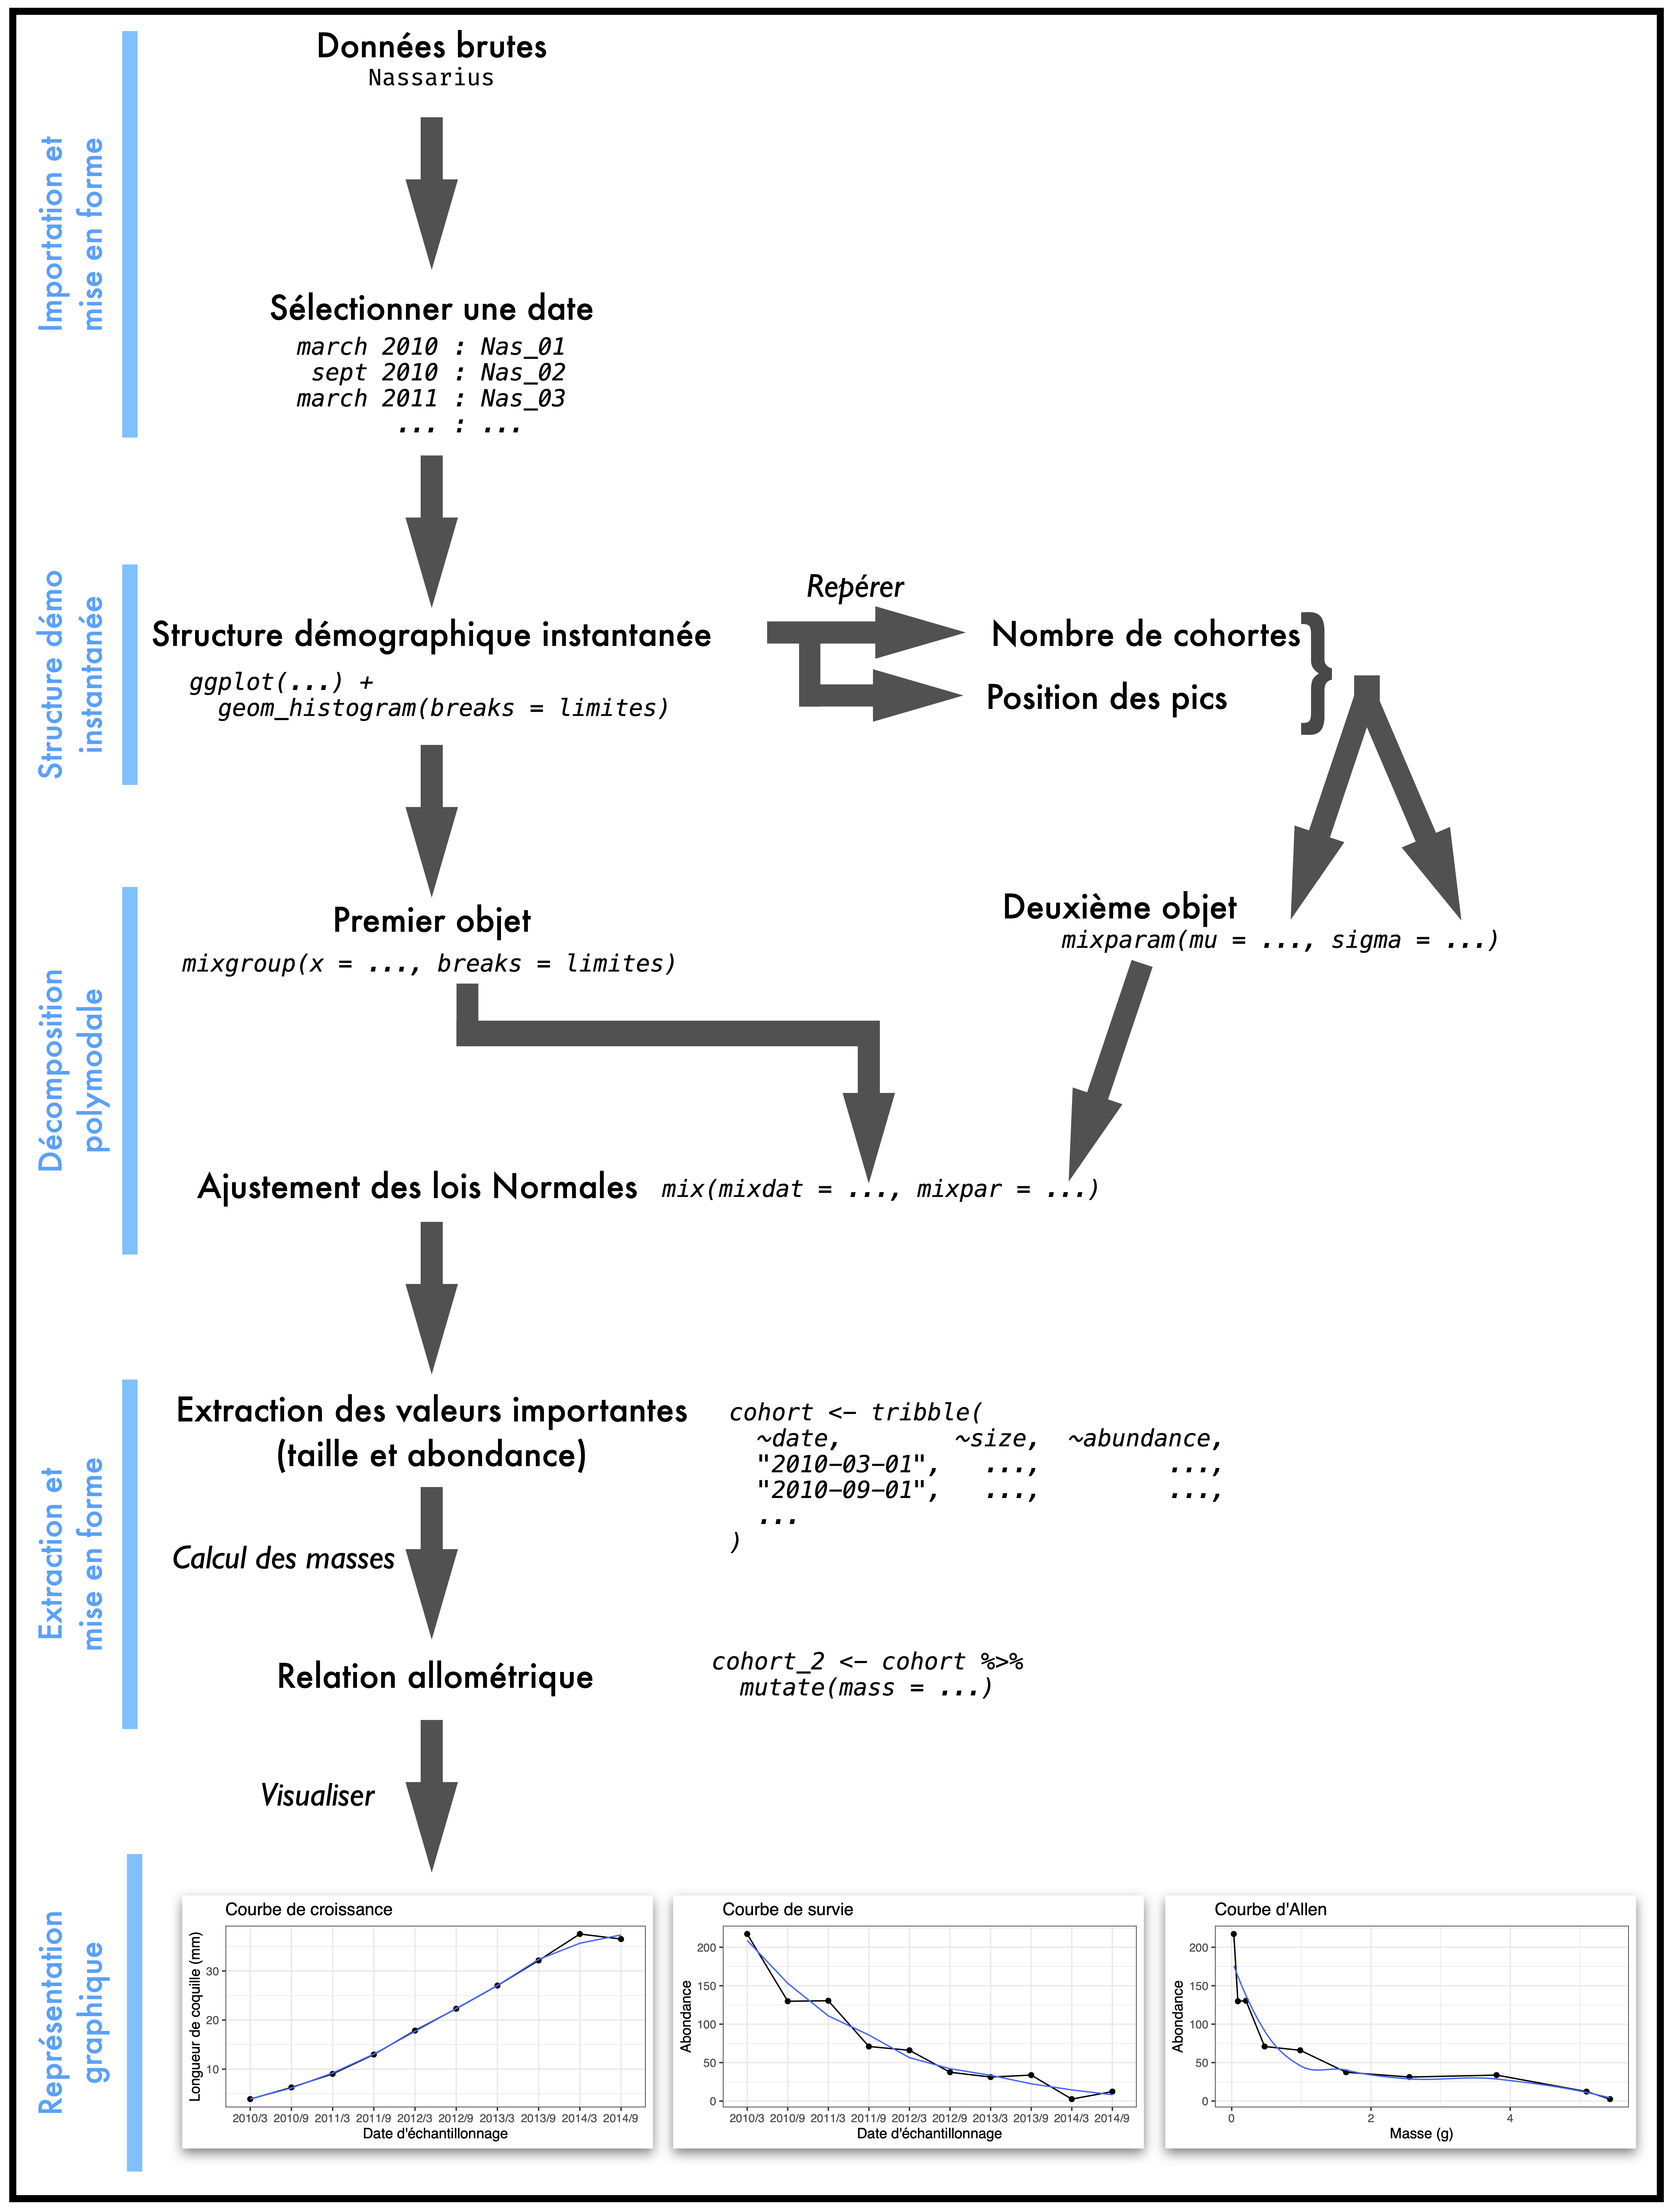
\includegraphics[keepaspectratio]{images/diagram.png}}

\end{figure*}%

Assurez vous que vous avez bien compris chaque étape de la méthode
décrite pour l'échantillonnage de mars 2010, et pourquoi on fait les
choses présentées ici dans l'ordre où on les fait. À ce stade, vous
devriez déjà avoir un script assez long qui devrait contenir la plupart
des commandes évoquées plus haut. Vous devriez donc pouvoir reproduire
ces étapes pour toutes les autres dates d'échantillonnage en faisant des
copier-coller et en modifiant quelques éléments précis (dates, nom des
objets, valeurs de tailles moyennes pour les cohortes, etc.). Attention
aussi à adopter une structure de script la plus clair possible, afin de
pouvoir corriger les éventuels bugs ou problèmes plus facilement.

Il ne vous reste donc plus qu'à reproduire ce travail pour les 9 autres
dates d'échantillonnage afin (i) de récupérer les valeurs d'abondance,
de taille et de masse moyenne des individus de la cohorte d'intérêt
(celle qui a été recrutée en mars 2010) et (ii) de compléter les 3
courbes que nous avons commencées plus haut.

Bon courage !

\bookmarksetup{startatroot}

\chapter{Systèmes dynamiques}\label{sec-dynam}

\section{Objectifs}\label{objectifs-3}

Dans ce chapitre, vous allez étudier plusieurs modèles dynamiques vus en
cours :

\begin{enumerate}
\def\labelenumi{\arabic{enumi}.}
\tightlist
\item
  modèle de mortalité exponentielle
\item
  modèle de croissance exponentielle
\item
  modèle de croissance logistique
\item
  modèle de Lotka-Volterra
\item
  modèles de compétition
\end{enumerate}

Pour cela, dans \texttt{RStudio}, vous devrez construire ces modèles en
utilisant des boucles \texttt{for} (dont nous détaillerons la syntaxe à
la Section~\ref{sec-for}) afin de décrire les variations d'abondance des
populations étudiées au cours du temps. Quand ces modèles seront
construits, vous devrez en faire varier les conditions initiales et les
valeurs des paramètres, afin d'observer le comportement du modèles dans
des conditions variées.

Pour chaque modèle cité plus haut, vous allez donc tout d'abord simuler
des données dans des conditions précises, en faire la représentation
graphique, puis modifier les paramètres du modèle pour comprendre
comment les différents termes (de croissance, de mortalité,
d'interaction\ldots) affectent les populations.

\section{Pré-requis}\label{sec-packages5}

Comme pour chaque nouveau chapitre, je vous conseille de travailler dans
un nouveau script que vous placerez dans votre répertoire de travail, et
dans une nouvelle session de travail (Menu
\texttt{Session\ \textgreater{}\ Restart\ R}). Inutile en revanche de
créer un nouveau \texttt{Rproject} : vous pouvez tout à fait avoir
plusieurs script dans le même répertoire de travail et pour un même
\texttt{Rproject}. Comme toujours, consultez
\href{https://besibo.github.io/BiometrieS3/01-R-basics.html\#sec-code}{le
livre en ligne du semestre 3} si vous ne savez plus comment faire.

Si vous êtes dans une nouvelle session de travail (ou que vous avez
quitté puis relancé \texttt{RStudio}), vous devrez penser à recharger en
mémoire les packages utiles. Dans ce chapitre, vous aurez uniquement
besoin des packages du \texttt{tidyverse} (Wickham 2023), en particulier
les package \texttt{dplyr} (Wickham et al. 2023), pour manipuler des
tableaux, et \texttt{ggplot2} ({Wickham, Chang, et al.} 2025) pour les
représentations graphiques.

\begin{Shaded}
\begin{Highlighting}[]
\FunctionTok{library}\NormalTok{(tidyverse)}
\end{Highlighting}
\end{Shaded}

Nous n'aurons pas besoin ici d'importer de données depuis des fichiers
externes : nous allons en effet générer directement des données à partir
de différents modèles démographiques vus en cours.

Comme toujours, je spécifie une fois pour toutes le thème que
j'utiliserai pour tous les graphiques de ce chapitre. Libre à vous de
choisir un thème différent ou de vous contenter du thème proposé par
défaut :

\begin{Shaded}
\begin{Highlighting}[]
\FunctionTok{theme\_set}\NormalTok{(}\FunctionTok{theme\_bw}\NormalTok{())}
\end{Highlighting}
\end{Shaded}

\section{\texorpdfstring{Les boucles
\texttt{for}}{Les boucles for}}\label{sec-for}

Dans tous les langages de programmation, les boucles permettent de
répéter automatiquement les mêmes actions un grand nombre de fois. Il
existe plusieurs types de boucles, mais les boucles \texttt{for} sont
les plus communes. Dans \texttt{R}, chaque boucle \texttt{for} possède 3
éléments :

\begin{enumerate}
\def\labelenumi{\arabic{enumi}.}
\item
  \textbf{La sortie}. Avant d'exécuter la boucle, vous devez toujours
  créer de façon explicite un objet qui contiendra les résultats des
  calculs effectués à l'intérieur de la boucle. Une bonne façon de créer
  un vecteur vide pour stocker des valeurs numériques consiste à
  utiliser la fonction \texttt{numeric()}
\item
  \textbf{La séquence} pour laquelle vous souhaitez ``faire tourner la
  boucle''. Dans une boucle \texttt{for}, vous devez indiquer un indice
  qui spécifie le nombre d'itérations que la boucle doit effectuer. Par
  exemple :

\begin{Shaded}
\begin{Highlighting}[]
\ControlFlowTok{for}\NormalTok{ (i }\ControlFlowTok{in} \DecValTok{1}\SpecialCharTok{:}\DecValTok{10}\NormalTok{)}
\end{Highlighting}
\end{Shaded}

  indique que les commandes qui figurent à l'intérieur de la boucle
  devront être exécutées 10 fois, une fois pour chaque valeur de
  \texttt{i}, c'est-à-dire 1, 2, 3\ldots{} jusqu'à 10. Pour chaque
  exécution des commandes de la boucle, l'indice \texttt{i} prendra donc
  une valeur différente comprise entre 1 et 10.
\item
  \textbf{Le corps de la boucle}. Il est constitué des commandes que
  l'on souhaite faire exécuter à la boucle, et il doit obligatoirement
  être encadré par des accolades \texttt{\{\ \}}.
\end{enumerate}

Voilà un exemple de boucle très simple :

\begin{Shaded}
\begin{Highlighting}[]
\CommentTok{\# Création d\textquotesingle{}un vecteur numérique vide}
\NormalTok{res }\OtherTok{\textless{}{-}} \FunctionTok{numeric}\NormalTok{()}

\CommentTok{\# Pour chaque valeur de i comprise entre 1 et 5}
\ControlFlowTok{for}\NormalTok{ (i }\ControlFlowTok{in} \DecValTok{1}\SpecialCharTok{:}\DecValTok{5}\NormalTok{) \{}
\NormalTok{  res[i] }\OtherTok{\textless{}{-}} \DecValTok{3} \SpecialCharTok{*}\NormalTok{ i }\SpecialCharTok{{-}} \DecValTok{1} \CommentTok{\# Calcule 3 * i {-} 1}
\NormalTok{\}}

\CommentTok{\# Affichage des résultats}
\NormalTok{res}
\end{Highlighting}
\end{Shaded}

\begin{verbatim}
[1]  2  5  8 11 14
\end{verbatim}

Les boucles peuvent faire des choses beaucoup plus complexes. Par
exemple, supposez que vous avez une première valeur de 100, et que vous
souhaitez diviser cette valeur par 2, puis que vous souhaitez diviser le
résultat par 2, et ainsi de suite, 10 fois. Voilà comment faire ça avec
une boucle \texttt{for} :

\begin{Shaded}
\begin{Highlighting}[]
\CommentTok{\# Création d\textquotesingle{}un vecteur numérique vide}
\NormalTok{res }\OtherTok{\textless{}{-}} \FunctionTok{numeric}\NormalTok{()}

\CommentTok{\# Stockage de la valeur initialle dans cet objet}
\NormalTok{res[}\DecValTok{1}\NormalTok{] }\OtherTok{\textless{}{-}} \DecValTok{100}

\CommentTok{\# Pour chaque valeur de i comprise entre 2 et 11}
\ControlFlowTok{for}\NormalTok{ (i }\ControlFlowTok{in} \DecValTok{2}\SpecialCharTok{:}\DecValTok{11}\NormalTok{) \{}
\NormalTok{  res[i] }\OtherTok{\textless{}{-}}\NormalTok{ res[i }\SpecialCharTok{{-}} \DecValTok{1}\NormalTok{] }\SpecialCharTok{/} \DecValTok{2}
\NormalTok{\}}

\CommentTok{\# Affichage des résultats}
\NormalTok{res}
\end{Highlighting}
\end{Shaded}

\begin{verbatim}
 [1] 100.00000000  50.00000000  25.00000000  12.50000000   6.25000000
 [6]   3.12500000   1.56250000   0.78125000   0.39062500   0.19531250
[11]   0.09765625
\end{verbatim}

Notez bien la position des accolades \texttt{\{} et \texttt{\}} dans le
code ci-dessus. Leur position est importante, de même que les sauts de
lignes. Notez aussi que dans cet exemple, \texttt{i} prend
successivement les valeurs 2, 3, 4, \ldots{} , 11, au lieu des valeurs
1, 2, 3, \ldots{} , 10. En effet, on connait déjà la première valeur de
\texttt{res}. On veut justement utiliser cette première valeur pour
calculer la deuxième, la troisième et ainsi de suite. Si on souhaite
répéter l'opération 10 fois de suite, il nous faut faire varier
\texttt{i} de 2 à 11 inclus. Ici, nous avons en réalité calculé
l'équation de récurrence suivante :

\[res_t = \frac{res_{t-1}}{2}\]

Vous savez maintenant comment fonctionnent les boucles \texttt{for} et
vous devriez donc pouvoir construire votre premier modèle dynamique.

\begin{tcolorbox}[enhanced jigsaw, arc=.35mm, bottomrule=.15mm, bottomtitle=1mm, breakable, colback=white, colbacktitle=quarto-callout-warning-color!10!white, colframe=quarto-callout-warning-color-frame, coltitle=black, left=2mm, leftrule=.75mm, opacityback=0, opacitybacktitle=0.6, rightrule=.15mm, title=\textcolor{quarto-callout-warning-color}{\faExclamationTriangle}\hspace{0.5em}{Attention}, titlerule=0mm, toprule=.15mm, toptitle=1mm]

Dans \texttt{R}, le premier élément d'un objet occupe la position
\texttt{{[}1{]}}. L'indice \texttt{{[}0{]}} n'existe pas. Il faut donc
faire attention à ce que les indices choisis pour \texttt{i} dans
l'expression \texttt{for\ (i\ in\ ...)} soient cohérents avec d'une part
la position dans l'objet qui stockera les résultats, et d'autre part
l'équation du système que l'on simule.

\end{tcolorbox}

\section{Modèle de mortalité exponentielle}\label{sec-mort}

Comme nous l'avons vu dans le cours, le modèle de mortalité
exponentielle est défini par l'équation suivante :

\[\frac{\mathrm{d}N}{\mathrm{d}t} = -mN\] Avec \(N\), l'abondance de la
population étudiée, \(t\), le temps et \(m\) le taux de mortalité
instantané. Pour coder ce modèle dans \texttt{RStudio}, vous devez vous
rappeler de \textbf{la signification} de cette équation différentielle.
Elle indique que dans un intervalle de temps très court \(\mathrm{d}t\),
\textbf{la variation de l'abondance de la population} \(\mathrm{d}N\)
vaut \(-mN\). Autrement dit, entre 2 temps d'observation successifs (par
exemple entre \(t\) et \(t + 1\), ou entre \(t - 1\) et \(t\)),
l'abondance de la population passe de \(N\) à \(N - mN\). Ce modèle peut
donc être décrit par l'équation de récurrence suivante :

\[N_{t+1} = N_t - m \times N_t\] ce qui est évidemment équivalent à

\[N_{t} = N_{t - 1} - m \times N_{t - 1}\] Cette dernière équation peut
se lire ainsi : l'abondance au temps \(t\) (\(N_t\)) est égale à
l'abondance au temps précédent \(N_{t-1}\), plus la variation
d'abondance entre 2 pas de temps successifs (\(-m\times N_{t-1}\)). Vous
devez utiliser cette équation pour construire le modèle de mortalité
exponentielle à l'intérieur d'une boucle \texttt{for} comme dans le
dernier exemple de la Section~\ref{sec-for}. Ici, on cherche donc à
déterminer la nouvelle valeur de la variable (\(N\) au temps \(t\)) en
utilisant la valeur de la même variable mais au temps précédent (\(N\)
au temps \(t-1\)).

Plusieurs étapes sont donc nécessaires :

\begin{enumerate}
\def\labelenumi{\arabic{enumi}.}
\item
  Créez un vecteur \texttt{N} qui sera utilisé pour stocker les
  résultats des calculs à chaque étape de simulation. Utilisez la
  commande suivante :

\begin{Shaded}
\begin{Highlighting}[]
\CommentTok{\# Création d\textquotesingle{}un vecteur numérique qui contiendra les résultats}
\NormalTok{N }\OtherTok{\textless{}{-}} \FunctionTok{numeric}\NormalTok{()}
\end{Highlighting}
\end{Shaded}
\item
  Fixez l'abondance initiale de la population à \(N_0 = 10\)
\item
  Fixez le taux de mortalité instantanée à \(m = 0.05\) (à chaque pas de
  temps, 5\% de la population disparaît)
\item
  Placez l'abondance initiale à la première position de \texttt{N}
\item
  Créez une boucle \texttt{for} pour calculer et placer dans \texttt{N}
  l'abondance de la population pour 100 pas de temps
\item
  Créez un tibble nommé \texttt{res} contenant 2 variables
  (\texttt{Generation} et \texttt{Abondance}) en utilisant cette
  commande :

\begin{Shaded}
\begin{Highlighting}[]
\CommentTok{\# Création d\textquotesingle{}un tibble où les résultats seront stockés}
\NormalTok{res }\OtherTok{\textless{}{-}} \FunctionTok{tibble}\NormalTok{(}\AttributeTok{Generation =} \DecValTok{0}\SpecialCharTok{:}\DecValTok{100}\NormalTok{, N)}
\end{Highlighting}
\end{Shaded}
\end{enumerate}

Si votre script est correct et qu'il s'exécute sans erreur, l'objet
\texttt{res} devrait contenir 101 lignes, avec 101 valeurs d'abondance.
Les premières lignes de \texttt{res} devraient contenir ces valeurs :

\begin{verbatim}
# A tibble: 101 x 2
   Generation     N
        <int> <dbl>
 1          0 10   
 2          1  9.5 
 3          2  9.02
 4          3  8.57
 5          4  8.15
 6          5  7.74
 7          6  7.35
 8          7  6.98
 9          8  6.63
10          9  6.30
# i 91 more rows
\end{verbatim}

Visualisez ces données avec \texttt{ggplot2}. Votre graphique devrait
ressembler à ceci :

{
\makeatletter
\def\LT@makecaption#1#2#3{%
  \noalign{\smash{\hbox{\kern\textwidth\rlap{\kern\marginparsep
  \parbox[t]{\marginparwidth}{%
    \footnotesize{%
      \vspace{(1.1\baselineskip)}
    #1{#2: }\ignorespaces #3}}}}}}%
    }
\makeatother

\begin{figure}

\sidecaption{\label{fig-mort}Modèle de mortalité exponentielle avec
\(N_0 = 10\) et \(m = 0.05\).}

\centering{

\pandocbounded{
\includegraphics[keepaspectratio]{06-DynamicSystems_files/figure-pdf/fig-mort-1.pdf}}

}

\end{figure}%

}

\begin{tcolorbox}[enhanced jigsaw, arc=.35mm, bottomrule=.15mm, bottomtitle=1mm, breakable, colback=white, colbacktitle=quarto-callout-caution-color!10!white, colframe=quarto-callout-caution-color-frame, coltitle=black, left=2mm, leftrule=.75mm, opacityback=0, opacitybacktitle=0.6, rightrule=.15mm, title=\textcolor{quarto-callout-caution-color}{\faFire}\hspace{0.5em}{Pour comprendre ce modèle\ldots{}}, titlerule=0mm, toprule=.15mm, toptitle=1mm]

Essayez d'utiliser plusieurs valeurs différentes pour \(N_0\) et
relancez tout le script. Que se passe-t-il quand \(N_0\) est très grand
? Est-ce normal ?

Enfin, essayez de changer la valeur de \(m\) et de relancer le script.
Faites des essais avec plusieurs valeurs. Qu'observe-t-on quand la
valeur de \(m\) se rapproche de 1 ? Est-ce normal ? Et que se passe-t-il
si \(m > 1\) ? Est-ce réaliste ? Pourquoi ? Mêmes questions avec
\(m = 2\) et \(m = 3\) ?

\end{tcolorbox}

\section{Modèle de croissance exponentielle}\label{sec-crois}

Comme nous l'avons vu dans le cours, le modèle de croissance
exponentielle est défini par l'équation suivante :

\[\frac{\mathrm{d}N}{\mathrm{d}t} = rN\] Avec \(N\), l'abondance de la
population étudiée, \(t\), le temps et \(r\) le taux de croissance
instantané. Pour coder ce modèle dans \texttt{RStudio}, vous devez vous
rappeler de \textbf{la signification} de cette équation différentielle.
Elle indique que dans un intervalle de temps très court \(\mathrm{d}t\),
\textbf{la variation de l'abondance de la population} \(\mathrm{d}N\)
vaut \(+rN\). Autrement dit, entre 2 temps d'observation successifs (par
exemple entre \(t\) et \(t + 1\), ou entre \(t - 1\) et \(t\)),
l'abondance de la population passe de \(N\) à \(N + rN\). Ce modèle peut
donc être décrit par l'équation de récurrence suivante :

\[N_{t+1} = N_t + r \times N_t\] ce qui est évidemment équivalent à

\[N_{t} = N_{t - 1} + r \times N_{t - 1}\] Cette dernière équation peut
se lire ainsi : l'abondance au temps \(t\) (\(N_t\)) est égale à
l'abondance au temps précédent \(N_{t-1}\), plus la variation
d'abondance entre 2 pas de temps successifs (\(+r\times N_{t-1}\)). Vous
devez utiliser cette équation pour construire le modèle de mortalité
exponentielle à l'intérieur d'une boucle \texttt{for} comme dans le
dernier exemple de la Section~\ref{sec-for}. Ici, on cherche donc à
déterminer la nouvelle valeur de la variable (\(N\) au temps \(t\)) en
utilisant la valeur de la même variable mais au temps précédent (\(N\)
au temps \(t-1\)).

Vous fixerez l'abondance initiale à \(N_0 = 5\) et le taux de croissance
instantané à \(r = 0.03\). Vous calculerez l'abondance de la population
pour 100 pas de temps. Vous devriez ainsi obtenir les résultats suivants
:

\begin{verbatim}
# A tibble: 101 x 2
   Generation     N
        <int> <dbl>
 1          0  5   
 2          1  5.15
 3          2  5.30
 4          3  5.46
 5          4  5.63
 6          5  5.80
 7          6  5.97
 8          7  6.15
 9          8  6.33
10          9  6.52
# i 91 more rows
\end{verbatim}

{
\makeatletter
\def\LT@makecaption#1#2#3{%
  \noalign{\smash{\hbox{\kern\textwidth\rlap{\kern\marginparsep
  \parbox[t]{\marginparwidth}{%
    \footnotesize{%
      \vspace{(1.1\baselineskip)}
    #1{#2: }\ignorespaces #3}}}}}}%
    }
\makeatother

\begin{figure}

\sidecaption{\label{fig-crois}Modèle de croissance exponentielle avec
\(N_0 = 5\) et \(r = 0.03\).}

\centering{

\pandocbounded{
\includegraphics[keepaspectratio]{06-DynamicSystems_files/figure-pdf/fig-crois-1.pdf}}

}

\end{figure}%

}

\begin{tcolorbox}[enhanced jigsaw, arc=.35mm, bottomrule=.15mm, bottomtitle=1mm, breakable, colback=white, colbacktitle=quarto-callout-caution-color!10!white, colframe=quarto-callout-caution-color-frame, coltitle=black, left=2mm, leftrule=.75mm, opacityback=0, opacitybacktitle=0.6, rightrule=.15mm, title=\textcolor{quarto-callout-caution-color}{\faFire}\hspace{0.5em}{Pour comprendre ce modèle\ldots{}}, titlerule=0mm, toprule=.15mm, toptitle=1mm]

Comme pour le modèle de mortalité exponentielle, essayez plusieurs
valeurs pour la condition initiale \(N_0\) et pour le paramètre du
modèle \(r\). Que se passe-t-il quand \(r = 1\) ? Examinez les première
valeurs d'abondance dans le tableau \texttt{res} pour vous faire une
meilleure idée. Est-ce réaliste ? Que se passe-t-il quand \(r > 1\) ?
Est-ce possible dans la nature ?

\end{tcolorbox}

\section{Modèle de croissance logistique}\label{sec-logist}

À partir du modèle de croissance exponentielle construit à la
Section~\ref{sec-crois}, vous devez maintenant construire un modèle de
croissance logistique qui est défini par l'équation suivante :

\[\frac{\mathrm{d}N}{\mathrm{d}t} = rN - \frac{r}{K}\times N^2\] Avec
\(N\), l'abondance de la population étudiée, \(t\), le temps, \(r\) le
taux de croissance instantané, et \(K\) la capacité biotique (ou
capacité de charge) du milieu. Comme toujours, commencez par écrire
cette équation sous forme d'une relation de récurrence :

\[N_{t} = N_{t - 1} + \cdots{}\] Rappelez-vous que la nouvelle abondance
(au temps \(t\)) est égale à l'ancienne (au temps \(t-1\)), plus la
variation d'abondance entre 2 pas de temps successifs, la formule de la
variation étant fournie par la formule
\(\frac{\mathrm{d}N}{\mathrm{d}t} = \cdots{}\)

Vous devez donc modifier le script de la Section~\ref{sec-crois} pour
ajouter le terme d'auto-limitation lié à l'environnement
\(\frac{r}{K}\times N^2\). Vous utiliserez les valeurs suivantes pour
les conditions initiales et les paramètres du modèle :

\begin{itemize}
\tightlist
\item
  \(N_0 = 1\)
\item
  \(r = 0.05\)
\item
  \(K = 80\)
\item
  durée de la simulation : 200 pas de temps
\end{itemize}

Vous devriez ainsi obtenir les résultats suivants :

\begin{verbatim}
# A tibble: 201 x 2
   Generation     N
        <int> <dbl>
 1          0  1   
 2          1  1.05
 3          2  1.10
 4          3  1.16
 5          4  1.21
 6          5  1.27
 7          6  1.33
 8          7  1.40
 9          8  1.47
10          9  1.54
# i 191 more rows
\end{verbatim}

{
\makeatletter
\def\LT@makecaption#1#2#3{%
  \noalign{\smash{\hbox{\kern\textwidth\rlap{\kern\marginparsep
  \parbox[t]{\marginparwidth}{%
    \footnotesize{%
      \vspace{(1.1\baselineskip)}
    #1{#2: }\ignorespaces #3}}}}}}%
    }
\makeatother

\begin{figure}

\sidecaption{\label{fig-logist}Modèle de croissance logistique avec
\(N_0 = 1\), \(r = 0.05\) et \(K = 80\).}

\centering{

\pandocbounded{
\includegraphics[keepaspectratio]{06-DynamicSystems_files/figure-pdf/fig-logist-1.pdf}}

}

\end{figure}%

}

\begin{tcolorbox}[enhanced jigsaw, arc=.35mm, bottomrule=.15mm, bottomtitle=1mm, breakable, colback=white, colbacktitle=quarto-callout-caution-color!10!white, colframe=quarto-callout-caution-color-frame, coltitle=black, left=2mm, leftrule=.75mm, opacityback=0, opacitybacktitle=0.6, rightrule=.15mm, title=\textcolor{quarto-callout-caution-color}{\faFire}\hspace{0.5em}{Pour comprendre ce modèle\ldots{}}, titlerule=0mm, toprule=.15mm, toptitle=1mm]

Modifiez les valeurs de \(N_0\), \(r\) et \(K\) l'une après l'autre,
pour comprendre comment chaque paramètre affecte la cinétique observée.
Que se passe-t-il quand \(N_0\) augmente ? Que se passe-t-il quand
\(N_0 > K\) ? Est-ce logique ? Pouvez-vous imaginer des situations
réalistes où \(N_0 > K\) ? Quelle est l'unité de \(K\) ?

Enfin, que se passe-t-il si le terme d'auto-limitation du milieu est
ajouté à la croissance exponentielle au lieu d'être soustrait ?
Expliquez.

\end{tcolorbox}

\section{Modèle prédateur-proie de Lotka-Volterra}\label{sec-lotka}

Vous allez maintenant étudier le modèle prédateur-proie tel que formulé
par Lotka et Volterra et dont les éuqations vous ont été décrites dans
le cours magistral de ``fonctionnement des écosystèmes'' :

\[
    \left\{
    \begin{array}{rcl}
        \displaystyle \frac{dX}{dt} & = & rX - \frac{r}{K}X^2 - c_1XY \\
        & & \\
        \displaystyle \frac{dY}{dt} & = & -mY + c_2XY
    \end{array}
    \right.
\] avec \(X\), l'abondance des proies, \(Y\), l'abondance des
prédateurs, \(r\) le taux de croissance instantanée des proies, \(K\) la
capacité biotique du milieu, \(m\) le taux de mortalité instantanée des
prédateurs, \(c_1\) l'effet négatif de la prédation sur les proies
(\emph{i.e.} la mortalité des proies causée par les rencontres avec les
prédateurs) et \(c_2\) l'effet positif de la prédation sur les
prédateurs (\emph{i.e.} la croissance de la population de prédateurs
causée par les rencontres avec les proies).

En utilisant la même démarche que précédemment, construisez un modèle de
Lotka-Volterra avec les valeurs suivantes :

\begin{itemize}
\tightlist
\item
  Abondance initiale des proies : \(X_0 = 1\)
\item
  Abondance initiale des prédateurs : \(Y_0 = 10\)
\item
  Taux de croissance instantanée des proies : \(r = 0.05\)
\item
  Taux de mortalité instantanée des prédateurs : \(m = 0.05\)
\item
  Capacité biotique du milieu : \(K = 50\)
\item
  Effet de la prédation sur les proies : \(c_1 = 0.01\)
\item
  Effet de la prédation sur les prédateurs : \(c_2 = 0.01\)
\item
  Durée de la simulation : 1000 pas de temps
\end{itemize}

Avec ce modèle, il vous faut calculer en parallèle l'abondance de 2
populations : celle des proies et celle des prédateurs.

\begin{tcolorbox}[enhanced jigsaw, arc=.35mm, bottomrule=.15mm, bottomtitle=1mm, breakable, colback=white, colbacktitle=quarto-callout-important-color!10!white, colframe=quarto-callout-important-color-frame, coltitle=black, left=2mm, leftrule=.75mm, opacityback=0, opacitybacktitle=0.6, rightrule=.15mm, title=\textcolor{quarto-callout-important-color}{\faExclamation}\hspace{0.5em}{Calcul simultané}, titlerule=0mm, toprule=.15mm, toptitle=1mm]

Attention : il est impossible de calculer d'abord toutes les abondances
des proies, puis ensuite toutes les abondances des prédateurs, dans 2
boucles \texttt{for} distinctes. À chaque nouveau pas de temps, au sein
d'une unique boucle \texttt{for}, il faut :

\begin{enumerate}
\def\labelenumi{\arabic{enumi}.}
\tightlist
\item
  calculer la nouvelle abondance des proies à partir de l'abondance des
  proies et des prédateurs au temps précédent
\item
  calculer la nouvelle abondance des prédateurs à partir de l'abondance
  des proies et des prédateurs au temps précédent
\end{enumerate}

\end{tcolorbox}

Au final, l'objet \texttt{res} qui contiendra les résultats de vos
simulation devra donc posséder 3 colonnes :

\begin{enumerate}
\def\labelenumi{\arabic{enumi}.}
\tightlist
\item
  Une colonne \texttt{Generation} contenant le numéro des étapes de
  simulation (les pas de temps)
\item
  Une colonne \texttt{X} contenant les abondances de la population de
  proies à chaque étape de simulation
\item
  Une colonne \texttt{Y} contenant les abondances de la population de
  prédateurs à chaque étape de simulation
\end{enumerate}

Avec ce tableau \texttt{res}, vous devriez pouvoir produire le diagramme
des phases suivants :

{
\makeatletter
\def\LT@makecaption#1#2#3{%
  \noalign{\smash{\hbox{\kern\textwidth\rlap{\kern\marginparsep
  \parbox[t]{\marginparwidth}{%
    \footnotesize{%
      \vspace{(1.1\baselineskip)}
    #1{#2: }\ignorespaces #3}}}}}}%
    }
\makeatother

\begin{figure}

\sidecaption{\label{fig-lotka}Modèle de Lotka-Volterra avec \(X_0 = 1\),
\(Y_0 = 10\), \(r = 0.05\), \(m = 0.05\), \(K = 80\) et
\(c_1 = c_2 = 0.01\). Le cercle violet indique les conditions
initiales.}

\centering{

\pandocbounded{
\includegraphics[keepaspectratio]{06-DynamicSystems_files/figure-pdf/fig-lotka-1.pdf}}

}

\end{figure}%

}

Pour faire ce graphique, vous aurez besoin d'utiliser la fonction
\texttt{geom\_path()} au lieu de \texttt{geom\_line()}. En effet,
\texttt{geom\_line()} relie les points d'un graphique par ordre
d'abscisse croissant :

\pandocbounded{
\includegraphics[keepaspectratio]{06-DynamicSystems_files/figure-pdf/unnamed-chunk-11-1.pdf}}

Ça n'est pas ce que nous voulons obtenir ! On souhaite relier les points
par ordre chronologique, donc dans l'ordre où ils apparaissent dans le
tableau \texttt{res}.

Enfin, pour mieux visualiser la dynamique de ces deux populations au
cours du temps, produisez le graphique suivant :

{
\makeatletter
\def\LT@makecaption#1#2#3{%
  \noalign{\smash{\hbox{\kern\textwidth\rlap{\kern\marginparsep
  \parbox[t]{\marginparwidth}{%
    \footnotesize{%
      \vspace{(1.1\baselineskip)}
    #1{#2: }\ignorespaces #3}}}}}}%
    }
\makeatother

\begin{figure}

\sidecaption{\label{fig-volterra}Modèle de Lotka-Volterra avec
\(X_0 = 1\), \(Y_0 = 10\), \(r = 0.05\), \(m = 0.05\), \(K = 80\) et
\(c_1 = c_2 = 0.01\).}

\centering{

\pandocbounded{
\includegraphics[keepaspectratio]{06-DynamicSystems_files/figure-pdf/fig-volterra-1.pdf}}

}

\end{figure}%

}

Pour produire ce graphique, vous aurez besoin de transformer le tableau
\texttt{res} en format long. Une colonne \texttt{Espece} devra contenir
soit \texttt{X}, soit \texttt{Y}, et une colonne \texttt{Abondance}
devra contenir toutes les valeurs d'abondance des 2 espèces. Si vous ne
savez plus comment faire, relisez
\href{https://besibo.github.io/BiometrieS4/01-dispersion.html\#sec-pivot}{le
chapitre 1.3} du livre en ligne du semestre 4. Voilà à quoi devraient
ressembler les premières lignes de votre tableau :

\begin{Shaded}
\begin{Highlighting}[]
\NormalTok{res\_long}
\end{Highlighting}
\end{Shaded}

\begin{verbatim}
# A tibble: 2,002 x 3
   Generation Espece Abondance
        <int> <chr>      <dbl>
 1          0 X          1    
 2          0 Y         10    
 3          1 X          0.949
 4          1 Y          9.6  
 5          2 X          0.904
 6          2 Y          9.21 
 7          3 X          0.866
 8          3 Y          8.83 
 9          4 X          0.832
10          4 Y          8.47 
# i 1,992 more rows
\end{verbatim}

\begin{tcolorbox}[enhanced jigsaw, arc=.35mm, bottomrule=.15mm, bottomtitle=1mm, breakable, colback=white, colbacktitle=quarto-callout-caution-color!10!white, colframe=quarto-callout-caution-color-frame, coltitle=black, left=2mm, leftrule=.75mm, opacityback=0, opacitybacktitle=0.6, rightrule=.15mm, title=\textcolor{quarto-callout-caution-color}{\faFire}\hspace{0.5em}{Pour comprendre ce modèle\ldots{}}, titlerule=0mm, toprule=.15mm, toptitle=1mm]

Expérimentez et tentez de répondre aux questions suivantes :

\begin{itemize}
\tightlist
\item
  Quelle sera l'issue de ce modèle prédateur-proie ? Augmentez la durée
  de simulation pour le prouver.
\item
  Quelles seront les abondances des proies et des prédateurs quand
  l'équilibre sera atteint ?
\item
  Modifiez la capacité biotique de la proie. QUe se passe-t-il quand
  vous l'augmentez ? Que se passe-t-il quand vous la diminuez ? Est-ce
  normal ? Est-ce ce à quoi vous vous attendiez ?
\item
  Que se passe-t-il quand vous modifiez les valeurs des autres
  paramètres du modèle (\(r\), \(m\), \(c_1\) et \(c_2\)) ?
\item
  Trouvez une combinaison de valeurs qui produisent un système à
  l'équilibre dynamique (\emph{i.e.} un système d'oscillations
  harmoniques avec un diagramme des phases présentant un attracteur
  cyclique ou une courbe fermée)
\item
  Est-ce que certaines combinaisons de paramètres produisent des
  résultats irréalistes ?
\end{itemize}

\end{tcolorbox}

\section{Modèle de compétition interspécifique}\label{sec-compet}

Dans sa forme la plus simple, on considère un système de compétition
entre 2 espèces présentant un modèle de croissance logistique. La
compétition ajoutera un terme de mortalité pour chaque espèce :

\[
    \left\{
    \begin{array}{rcl}
        \displaystyle \frac{dX}{dt} & = & r_1X - \frac{r_1}{K_1}X^2 - c_1XY \\
        & & \\
        \displaystyle \frac{dY}{dt} & = & r_2Y - \frac{r_2}{K_2}Y^2 - c_2XY
    \end{array}
    \right.
\]

avec \(X\) et \(Y\) l'abondance des deux espèces, \(r_1\) et \(r_2\) les
taux de croissance instantanée des deux espèces, \(K_1\) et \(K_2\) les
capacités biotiques pour les 2 espèces, et \(c_1\) et \(c_2\) les effets
négatifs de la compétition sur chacune des 2 espèces (\emph{i.e.} la
mortalité causée par les rencontres entre les deux espèces en
compétition).

En modifiant le système prédateur-proie précédent, codez ce système de
compétition et essayez de trouver une combinaison de paramètres et de
valeurs initiales permettant de reproduire les 4 situations décrites en
cours :

\begin{enumerate}
\def\labelenumi{\arabic{enumi}.}
\tightlist
\item
  Deux espèces très compétitives (avec différentes abondances
  initiales). Retrouvez-vous la ligne de catastrophe ?
\end{enumerate}

{
\makeatletter
\def\LT@makecaption#1#2#3{%
  \noalign{\smash{\hbox{\kern\textwidth\rlap{\kern\marginparsep
  \parbox[t]{\marginparwidth}{%
    \footnotesize{%
      \vspace{(1.1\baselineskip)}
    #1{#2: }\ignorespaces #3}}}}}}%
    }
\makeatother

\begin{figure}

\sidecaption{\label{fig-compet_strong}Diagramme des phases de 2 espèces
en compétition : 2 espèces très compétitives avec des conditions
initiales différentes.}

\centering{

\pandocbounded{
\includegraphics[keepaspectratio]{06-DynamicSystems_files/figure-pdf/fig-compet_strong-1.pdf}}

}

\end{figure}%

}

\begin{enumerate}
\def\labelenumi{\arabic{enumi}.}
\setcounter{enumi}{1}
\tightlist
\item
  Deux espèces très peu compétitives
\item
  Première espèce plus compétitive que la seconde
\item
  Seconde espèce plus compétitive que la première
\end{enumerate}

{
\makeatletter
\def\LT@makecaption#1#2#3{%
  \noalign{\smash{\hbox{\kern\textwidth\rlap{\kern\marginparsep
  \parbox[t]{\marginparwidth}{%
    \footnotesize{%
      \vspace{(1.1\baselineskip)}
    #1{#2: }\ignorespaces #3}}}}}}%
    }
\makeatother

\begin{figure}

\sidecaption{\label{fig-compet}Diagramme des phases de 2 espèces en
compétition : 3 situations distinctes.}

\centering{

\pandocbounded{
\includegraphics[keepaspectratio]{06-DynamicSystems_files/figure-pdf/fig-compet-1.pdf}}

}

\end{figure}%

}

\begin{tcolorbox}[enhanced jigsaw, arc=.35mm, bottomrule=.15mm, bottomtitle=1mm, breakable, colback=white, colbacktitle=quarto-callout-caution-color!10!white, colframe=quarto-callout-caution-color-frame, coltitle=black, left=2mm, leftrule=.75mm, opacityback=0, opacitybacktitle=0.6, rightrule=.15mm, title=\textcolor{quarto-callout-caution-color}{\faFire}\hspace{0.5em}{Pour comprendre ce modèle\ldots{}}, titlerule=0mm, toprule=.15mm, toptitle=1mm]

Attention à l'échelle des axes de vos graphiques. Pour bien comprendre
ce qui se passe et retrouver les figures schématiques vues en cours,
vous devez tenter de replacer les graphique produits ici dans un plan
plus large.

Notez aussi que contrairement au modèle prédateur-proie, les modèles de
compétition ne font pas apparaître de cycles sur les diagrammes des
phases. L'évolution des abondances au cours du temps ne fait donc jamais
apparaître d'oscillations.

\end{tcolorbox}

\section{Modèles à 3 espèces}\label{sec-multispe}

Sur la base des chapitres précédents, vous devriez maintenant pouvoir
construire des modèles plus complexes, par exemple à 3 espèces en
compétition, ou à 3 espèces dont 2 proies en compétition et une espèce
de prédateur. La clé est ici de ne pas oublier de termes lorsque l'on
construit le modèle : pour chaque espèce supplémentaire dans le modèle,
la complexité augmente singulièrement. En effet, une espèce signifie une
équation de plus dans le système, mais également des termes
d'interaction supplémentaires dans les équations déjà existantes.

Par exemple, si on considère un système dans lequel 3 espèces sont
présentes, deux espèces de proies en compétition et un prédateur, voilà
à quoi ressemblent le système d'équations :

\[
    \left\{
    \begin{array}{rcl}
        \displaystyle \frac{dX}{dt} & = & r_1X - \frac{r_1}{K_1}X^2 - c_{12}XY - c_{13}XZ \\
        & & \\
        \displaystyle \frac{dY}{dt} & = & r_2Y - \frac{r_2}{K_2}Y^2 - c_{21}XY - c_{23}YZ \\
        & & \\
        \displaystyle \frac{dZ}{dt} & = & -mZ + c_{31}XZ + c_{32}YZ
    \end{array}
    \right.
\]

Ce système de 3 équations comprend maintenant 11 paramètres : \(r_1\),
\(r_2\), \(K_1\), \(K_2\), \(m\), \(c_{12}\), \(c_{21}\), \(c_{13}\),
\(c_{23}\), \(c_{31}\) et \(c_{32}\).

Essayez de coder ce système et de produire une figure telle que la
Figure~\ref{fig-3spe}.

{
\makeatletter
\def\LT@makecaption#1#2#3{%
  \noalign{\smash{\hbox{\kern\textwidth\rlap{\kern\marginparsep
  \parbox[t]{\marginparwidth}{%
    \footnotesize{%
      \vspace{(1.1\baselineskip)}
    #1{#2: }\ignorespaces #3}}}}}}%
    }
\makeatother

\begin{figure}

\sidecaption{\label{fig-3spe}Évolution de l'abondance de 2 espèces de
proies en compétition et d'une espèce prédatrice. Ici, les 2 espèces de
proies ont les mêmes caractéristiques démographiques et sont peu
compétitives. Le prédateur a un impact plus important sur l'espèce de
proie 2 (abondance Y) et conduit donc à son extinction.}

\centering{

\pandocbounded{
\includegraphics[keepaspectratio]{06-DynamicSystems_files/figure-pdf/fig-3spe-1.pdf}}

}

\end{figure}%

}

\begin{tcolorbox}[enhanced jigsaw, arc=.35mm, bottomrule=.15mm, bottomtitle=1mm, breakable, colback=white, colbacktitle=quarto-callout-caution-color!10!white, colframe=quarto-callout-caution-color-frame, coltitle=black, left=2mm, leftrule=.75mm, opacityback=0, opacitybacktitle=0.6, rightrule=.15mm, title=\textcolor{quarto-callout-caution-color}{\faFire}\hspace{0.5em}{Pour comprendre ce modèle\ldots{}}, titlerule=0mm, toprule=.15mm, toptitle=1mm]

Expérimentez et tentez de répondre aux questions suivantes :

\begin{itemize}
\tightlist
\item
  Pouvez-vous trouver une combinaison de paramètres conduisant à la
  coexistence des 3 espèces ?
\item
  Pouvez-vous trouver une combinaison de paramètres conduisant à la
  coexistence de 2 des 3 espèces ?
\item
  Que se passe-t-il si on augmente légèrement la capacité biotique de la
  première espèce ? À quelle espèce cela devrait profiter le plus ?
  Est-ce ce que l'on observe ? Cela vous paraît-il logique ?
\item
  Dans le système d'équation ci-dessus, êtes-vous capables d'identifier
  à quoi correspondent chacun des termes ? Quels sont les termes qui
  rendent comptent de la compétition ? Quels sont les termes qui rendent
  compte de la prédation ?
\end{itemize}

\end{tcolorbox}

\bookmarksetup{startatroot}

\chapter{Les Chaînes de Markov}\label{sec-markov}

\section{Pré-requis}\label{sec-packages6}

Comme pour chaque nouveau chapitre, je vous conseille de travailler dans
un nouveau script que vous placerez dans votre répertoire de travail, et
dans une nouvelle session de travail (Menu
\texttt{Session\ \textgreater{}\ Restart\ R}). Inutile en revanche de
créer un nouveau \texttt{Rproject} : vous pouvez tout à fait avoir
plusieurs script dans le même répertoire de travail et pour un même
\texttt{Rproject}. Comme toujours, consultez
\href{https://besibo.github.io/BiometrieS3/01-R-basics.html\#sec-code}{le
livre en ligne du semestre 3} si vous ne savez plus comment faire.

Si vous êtes dans une nouvelle session de travail (ou que vous avez
quitté puis relancé \texttt{RStudio}), vous devrez penser à recharger en
mémoire les packages utiles. Dans ce chapitre, vous aurez uniquement
besoin des packages du \texttt{tidyverse} (Wickham 2023), en particulier
les package \texttt{dplyr} (Wickham et al. 2023), pour manipuler des
tableaux, et \texttt{ggplot2} ({Wickham, Chang, et al.} 2025) pour les
représentations graphiques. Vous pourrez aussi avoir besoin du package
\texttt{scales} (Wickham, Pedersen, et al. 2025) pour améliorer la mise
en forme des axes des graphiques produits

\begin{Shaded}
\begin{Highlighting}[]
\FunctionTok{library}\NormalTok{(tidyverse)}
\FunctionTok{library}\NormalTok{(scales)}
\end{Highlighting}
\end{Shaded}

Nous n'aurons pas besoin ici d'importer de données depuis des fichiers
externes : nous allons en effet générer directement des données à partir
d'une chaîne de Markov.

Comme toujours, je spécifie une fois pour toutes le thème que
j'utiliserai pour tous les graphiques de ce chapitre. Libre à vous de
choisir un thème différent ou de vous contenter du thème proposé par
défaut :

\begin{Shaded}
\begin{Highlighting}[]
\FunctionTok{theme\_set}\NormalTok{(}\FunctionTok{theme\_bw}\NormalTok{())}
\end{Highlighting}
\end{Shaded}

\section{\texorpdfstring{Les matrices dans
\texttt{R}}{Les matrices dans R}}\label{les-matrices-dans-r}

Lors de votre découverte du logiciel \texttt{R}, de son fonctionnement
et de sa syntaxe, vous avez appris qu'il existe plusieurs types d'objets
que l'on peut créer et manipuler : des vecteurs, des facteurs, des
data.frames ou tibbles, des listes, etc. L'un des types d'objets que
nous n'avons pas encore décrit est la matrice.

Dans \texttt{R}, une matrice est un tableau dans lequel chaque cellule
contient des éléments du même type. Contrairement aux data.frames et aux
tibbles, une matrice ne peut donc pas avoir des chiffres dans une
colonne, et des chaînes de caractères ou des vrais-faux dans une autre.
De ce point de vue, une matrice est donc similaire à un vecteur qui ne
peut contenir que des éléments qui sont tous du même type. Mais comme un
data.frame ou un tibble, et contrairement à un vecteur, une matrice
possède des dimensions : un nombre de lignes et un nombre de colonnes.

Les matrices sont donc des objets qui possèdent des points communs et
des différences, avec les vecteurs et avec les data.frames ou tibbles.

\subsection{Création}\label{cruxe9ation}

La façon la plus simple de créer une matrice est d'utiliser la fonction
\texttt{matrix()}. Cette fonction possède de nombreux arguments et vous
devrez au moins renseigner les suivants :

\begin{itemize}
\tightlist
\item
  \texttt{data} : quelles données souhaitez vous placer dans la matrice.
  Il peut s'agir d'une unique valeur si vous souhaitez que toutes les
  cellules de la matrice contiennent la même chose. En général, il
  s'agit d'un vecteur contenant les éléments que l'on souhaite placer
  dans la matrice.
\item
  \texttt{nrow} : combien de lignes la matrice que vous souhaitez créer
  devra-t-elle contenir ?
\item
  \texttt{ncol} : combien de colonnes la matrice que vous souhaitez
  créer devra-t-elle contenir ?
\item
  \texttt{byrow} : souhaitez-vous que les données fournies dans
  \texttt{data} soient remplies en lignes (\texttt{byrow\ =\ TRUE}) ou
  en colonnes (\texttt{byrow\ =\ FALSE}, c'est le choix par défaut) dans
  la matrice ?
\end{itemize}

En général, on renseigne donc systématiquement \texttt{data}, et soit
\texttt{nrow}, soit \texttt{ncol}. Il n'est pas nécessaire de renseigner
à la fois \texttt{nrow} et \texttt{ncol} puisque \texttt{R} est capable
de déterminer l'un des deux automatiquement selon la taille du vecteur
que vous avez fourni à \texttt{data}. Par exemple, si vous fournissez un
vecteur de 15 éléments à data, et que vous indiquez \texttt{nrow\ =\ 3},
\texttt{R} produira automatiquement une matrice de 3 lignes et 5
colonnes. Cela suppose évidemment que la longueur du vecteur fourni soit
compatible avec les dimensions de la matrice que vous envisagez.

Vous pouvez évidemment spécifier explicitement le nombre de lignes et le
nombre de colonnes souhaitées, mais alors la longueur du vecteur fourni
devra être parfaitement compatible avec les dimensions de la matrice
envisagée. Par exemple, si vous souhaitez une matrice de 4 lignes et 4
colonnes (soit 16 cellules), vous devrez fournir exactement 16 valeurs
dans le vecteur transmis à l'argument \texttt{data}. Si vous en
fournissez plus ou moins, des choses inattendues peuvent se produire :

\begin{itemize}
\tightlist
\item
  si vous fournissez trop de valeurs, les valeurs en trop ne seront pas
  intégrées à la matrice, votre vecteur sera donc tronqué après la
  seizième valeur
\item
  si vous fournissez trop peu de valeurs, le recyclage sera utilisé pour
  combler la matrice qui ne peut pas avoir de cellule vide : les
  première valeurs du vecteur seront réutilisées jusqu'à ce que la
  matrice soit remplie, et un message d'avertissement vous sera renvoyé.
\end{itemize}

Voici quelques exemples :

\begin{Shaded}
\begin{Highlighting}[]
\CommentTok{\# Création d\textquotesingle{}un vecteur de 8 éléments}
\NormalTok{a }\OtherTok{\textless{}{-}} \FunctionTok{c}\NormalTok{(}\DecValTok{1}\NormalTok{, }\DecValTok{5}\NormalTok{, }\DecValTok{6}\NormalTok{, }\DecValTok{9}\NormalTok{, }\DecValTok{10}\NormalTok{, }\DecValTok{5}\NormalTok{, }\DecValTok{4}\NormalTok{, }\DecValTok{2}\NormalTok{)  }\CommentTok{\# 8 éléments}

\CommentTok{\# Création d\textquotesingle{}une matrice de 2 lignes et 4 colonnes}
\FunctionTok{matrix}\NormalTok{(}\AttributeTok{data =}\NormalTok{ a, }\AttributeTok{nrow =} \DecValTok{2}\NormalTok{)}
\end{Highlighting}
\end{Shaded}

\begin{verbatim}
     [,1] [,2] [,3] [,4]
[1,]    1    6   10    4
[2,]    5    9    5    2
\end{verbatim}

\begin{Shaded}
\begin{Highlighting}[]
\CommentTok{\# Une autre façon de créer la même matrice}
\FunctionTok{matrix}\NormalTok{(}\AttributeTok{data =}\NormalTok{ a, }\AttributeTok{ncol =} \DecValTok{4}\NormalTok{)}
\end{Highlighting}
\end{Shaded}

\begin{verbatim}
     [,1] [,2] [,3] [,4]
[1,]    1    6   10    4
[2,]    5    9    5    2
\end{verbatim}

Si la longueur du vecteur contenant les données n'est pas compatible
avec les dimensions voulues pour la matrice, il faut spécifier les
nombres de lignes et de colonnes de façon explicite, et un message
d'avertissement est renvoyé.

\begin{Shaded}
\begin{Highlighting}[]
\CommentTok{\# Pour créer une matrice de 3 lignes et 4 colonnes, il faut spécifier }
\CommentTok{\# explicitement nrow et ncol}
\FunctionTok{matrix}\NormalTok{(}\AttributeTok{data =}\NormalTok{ a, }\AttributeTok{nrow =} \DecValTok{3}\NormalTok{, }\AttributeTok{ncol =} \DecValTok{4}\NormalTok{)}
\end{Highlighting}
\end{Shaded}

\begin{verbatim}
Warning in matrix(data = a, nrow = 3, ncol = 4): data length [8] is not a
sub-multiple or multiple of the number of rows [3]
\end{verbatim}

\begin{verbatim}
     [,1] [,2] [,3] [,4]
[1,]    1    9    4    5
[2,]    5   10    2    6
[3,]    6    5    1    9
\end{verbatim}

Ici, les premières valeurs du vecteur \texttt{a} ont été recyclées (1,
5, 6 et 9) pour remplir toutes les cellules de la matrice.

Dans tous les exemples ci-dessus, les chiffres contenus dans le vecteur
\texttt{a} ont été remplis en colonnes dans la matrice. Pour remplir la
matrice en lignes, on indique \texttt{byrow\ =\ TRUE} :

\begin{Shaded}
\begin{Highlighting}[]
\FunctionTok{matrix}\NormalTok{(}\AttributeTok{data =}\NormalTok{ a, }\AttributeTok{nrow =} \DecValTok{2}\NormalTok{, }\AttributeTok{byrow =} \ConstantTok{TRUE}\NormalTok{)}
\end{Highlighting}
\end{Shaded}

\begin{verbatim}
     [,1] [,2] [,3] [,4]
[1,]    1    5    6    9
[2,]   10    5    4    2
\end{verbatim}

\begin{Shaded}
\begin{Highlighting}[]
\FunctionTok{matrix}\NormalTok{(}\AttributeTok{data =}\NormalTok{ a, }\AttributeTok{ncol =} \DecValTok{4}\NormalTok{, }\AttributeTok{byrow =} \ConstantTok{TRUE}\NormalTok{)}
\end{Highlighting}
\end{Shaded}

\begin{verbatim}
     [,1] [,2] [,3] [,4]
[1,]    1    5    6    9
[2,]   10    5    4    2
\end{verbatim}

\begin{Shaded}
\begin{Highlighting}[]
\FunctionTok{matrix}\NormalTok{(}\AttributeTok{data =}\NormalTok{ a, }\AttributeTok{nrow =} \DecValTok{3}\NormalTok{, }\AttributeTok{ncol =} \DecValTok{4}\NormalTok{, }\AttributeTok{byrow =} \ConstantTok{TRUE}\NormalTok{)}
\end{Highlighting}
\end{Shaded}

\begin{verbatim}
Warning in matrix(data = a, nrow = 3, ncol = 4, byrow = TRUE): data length [8]
is not a sub-multiple or multiple of the number of rows [3]
\end{verbatim}

\begin{verbatim}
     [,1] [,2] [,3] [,4]
[1,]    1    5    6    9
[2,]   10    5    4    2
[3,]    1    5    6    9
\end{verbatim}

Et bien sûr, comme vous le savez maintenant, si vous souhaitez pouvoir
réutiliser les matrices créées avec la fonction \texttt{matrix()}, vous
devez leur donner un nom avec l'oérateur \texttt{\textless{}-} :

\begin{Shaded}
\begin{Highlighting}[]
\NormalTok{mat }\OtherTok{\textless{}{-}} \FunctionTok{matrix}\NormalTok{(}\AttributeTok{data =}\NormalTok{ a, }\AttributeTok{nrow =} \DecValTok{3}\NormalTok{, }\AttributeTok{ncol =} \DecValTok{4}\NormalTok{, }\AttributeTok{byrow =} \ConstantTok{TRUE}\NormalTok{)}
\end{Highlighting}
\end{Shaded}

\begin{verbatim}
Warning in matrix(data = a, nrow = 3, ncol = 4, byrow = TRUE): data length [8]
is not a sub-multiple or multiple of the number of rows [3]
\end{verbatim}

\begin{Shaded}
\begin{Highlighting}[]
\NormalTok{mat}
\end{Highlighting}
\end{Shaded}

\begin{verbatim}
     [,1] [,2] [,3] [,4]
[1,]    1    5    6    9
[2,]   10    5    4    2
[3,]    1    5    6    9
\end{verbatim}

\subsection{Produit matriciel}\label{produit-matriciel}

Le produit matriciel est l'opération qui permet de multiplier 2 matrices
entre elles, ou de multiplier une matrice par un vecteur. Comme nous
l'avons vu en cours, les dimension des objets que l'on multiplie sont
importantes.

\begin{tcolorbox}[enhanced jigsaw, arc=.35mm, bottomrule=.15mm, bottomtitle=1mm, breakable, colback=white, colbacktitle=quarto-callout-important-color!10!white, colframe=quarto-callout-important-color-frame, coltitle=black, left=2mm, leftrule=.75mm, opacityback=0, opacitybacktitle=0.6, rightrule=.15mm, title=\textcolor{quarto-callout-important-color}{\faExclamation}\hspace{0.5em}{Produit matriciel}, titlerule=0mm, toprule=.15mm, toptitle=1mm]

Si \(A\) et \(B\) sont deux matrices, le produit matriciel \(A\times B\)
n'est possible que si le nombre de colonnes de \(A\) est égal au nombre
de lignes de \(B\).

Par ailleurs, sauf cas particulier, \(A\times B \neq B\times A\)

\end{tcolorbox}

Dans \texttt{R}, l'opérateur qui permet d'effectuer un produit matriciel
est \texttt{\%*\%}.

\begin{Shaded}
\begin{Highlighting}[]
\CommentTok{\# Création d\textquotesingle{}une matrice A}
\NormalTok{A }\OtherTok{\textless{}{-}} \FunctionTok{matrix}\NormalTok{(}\DecValTok{1}\SpecialCharTok{:}\DecValTok{15}\NormalTok{, }\AttributeTok{nrow =} \DecValTok{5}\NormalTok{)}
\NormalTok{A}
\end{Highlighting}
\end{Shaded}

\begin{verbatim}
     [,1] [,2] [,3]
[1,]    1    6   11
[2,]    2    7   12
[3,]    3    8   13
[4,]    4    9   14
[5,]    5   10   15
\end{verbatim}

\begin{Shaded}
\begin{Highlighting}[]
\FunctionTok{dim}\NormalTok{(A)}
\end{Highlighting}
\end{Shaded}

\begin{verbatim}
[1] 5 3
\end{verbatim}

\begin{Shaded}
\begin{Highlighting}[]
\CommentTok{\# Création d\textquotesingle{}une matrice B}
\NormalTok{B }\OtherTok{\textless{}{-}} \FunctionTok{matrix}\NormalTok{(}\DecValTok{1}\SpecialCharTok{:}\DecValTok{15}\NormalTok{, }\AttributeTok{ncol =} \DecValTok{5}\NormalTok{)}
\NormalTok{B}
\end{Highlighting}
\end{Shaded}

\begin{verbatim}
     [,1] [,2] [,3] [,4] [,5]
[1,]    1    4    7   10   13
[2,]    2    5    8   11   14
[3,]    3    6    9   12   15
\end{verbatim}

\begin{Shaded}
\begin{Highlighting}[]
\FunctionTok{dim}\NormalTok{(B)}
\end{Highlighting}
\end{Shaded}

\begin{verbatim}
[1] 3 5
\end{verbatim}

\begin{Shaded}
\begin{Highlighting}[]
\CommentTok{\# Produit matriciel A * B}
\NormalTok{A }\SpecialCharTok{\%*\%}\NormalTok{ B}
\end{Highlighting}
\end{Shaded}

\begin{verbatim}
     [,1] [,2] [,3] [,4] [,5]
[1,]   46  100  154  208  262
[2,]   52  115  178  241  304
[3,]   58  130  202  274  346
[4,]   64  145  226  307  388
[5,]   70  160  250  340  430
\end{verbatim}

\begin{Shaded}
\begin{Highlighting}[]
\CommentTok{\# Produit matriciel B * A}
\NormalTok{B }\SpecialCharTok{\%*\%}\NormalTok{ A}
\end{Highlighting}
\end{Shaded}

\begin{verbatim}
     [,1] [,2] [,3]
[1,]  135  310  485
[2,]  150  350  550
[3,]  165  390  615
\end{verbatim}

Vous constatez ici que les dimensions de la matrice obtenue sont
variables et dépendent du sens du produit matriciel et des dimensions
des matrices multipliées. Multiplier 2 matrices dont les dimensions sont
incompatibles fait apparaître un message d'erreur :

\begin{Shaded}
\begin{Highlighting}[]
\CommentTok{\# Création d\textquotesingle{}une matrice C (4 lignes et 3 colonnes)}
\NormalTok{C }\OtherTok{\textless{}{-}} \FunctionTok{matrix}\NormalTok{(}\DecValTok{1}\SpecialCharTok{:}\DecValTok{12}\NormalTok{, }\AttributeTok{ncol =} \DecValTok{3}\NormalTok{)}
\NormalTok{C}
\end{Highlighting}
\end{Shaded}

\begin{verbatim}
     [,1] [,2] [,3]
[1,]    1    5    9
[2,]    2    6   10
[3,]    3    7   11
[4,]    4    8   12
\end{verbatim}

\begin{Shaded}
\begin{Highlighting}[]
\CommentTok{\# Affichage de la matrice A (5 lignes et 3 colonnes)}
\NormalTok{A}
\end{Highlighting}
\end{Shaded}

\begin{verbatim}
     [,1] [,2] [,3]
[1,]    1    6   11
[2,]    2    7   12
[3,]    3    8   13
[4,]    4    9   14
[5,]    5   10   15
\end{verbatim}

\begin{Shaded}
\begin{Highlighting}[]
\CommentTok{\# Calcul des produits matriciels : impossibles !}
\NormalTok{A }\SpecialCharTok{\%*\%}\NormalTok{ C}
\end{Highlighting}
\end{Shaded}

\begin{verbatim}
Error in A %*% C: non-conformable arguments
\end{verbatim}

\begin{Shaded}
\begin{Highlighting}[]
\NormalTok{C }\SpecialCharTok{\%*\%}\NormalTok{ A}
\end{Highlighting}
\end{Shaded}

\begin{verbatim}
Error in C %*% A: non-conformable arguments
\end{verbatim}

Enfin, il est tout à fait possible d'effectuer un produit matriciel
entre une vecteur et une matrice. Dans \texttt{R}, les vecteurs n'ont
pas de dimension, mais ils ont une longueur (\emph{i.e.} un nombre
d'éléments), que l'on peut afficher avec la fonction \texttt{length()}.
Lorsque l'on effectue un produit matriciel impliquant un vecteur, le
vecteur est automatiquement transformé soit en vecteur ligne (une
matrice d'une seule ligne) soit en vecteur colonne (une matrice d'une
seule colonne, voir le cours de ``Fonctionnement des écosystèmes'') :

\begin{itemize}
\tightlist
\item
  Si les vecteur est à gauche (\texttt{vec\ \%*\%\ mat}), il est
  transformé en vecteur ligne. Pour que le produit matriciel puisse être
  calculé, il faut alors que le nombre d'éléments de \texttt{vec} soit
  égal au nombre de lignes de \texttt{mat}.
\item
  Si les vecteur est à droite (\texttt{mat\ \%*\%\ vec}), il est
  transformé en vecteur colonne. Pour que le produit matriciel puisse
  être calculé, il faut alors que le nombre d'éléments de \texttt{vec}
  soit égal au nombre de colonnes de \texttt{mat}.
\end{itemize}

\begin{Shaded}
\begin{Highlighting}[]
\CommentTok{\# Création d\textquotesingle{}un vecteur}
\NormalTok{vec }\OtherTok{\textless{}{-}} \FunctionTok{c}\NormalTok{(}\DecValTok{2}\NormalTok{, }\DecValTok{4}\NormalTok{, }\DecValTok{3}\NormalTok{)}
\NormalTok{vec}
\end{Highlighting}
\end{Shaded}

\begin{verbatim}
[1] 2 4 3
\end{verbatim}

\begin{Shaded}
\begin{Highlighting}[]
\CommentTok{\# Création d\textquotesingle{}une matrice D : 3 lignes et 2 colonnes}
\NormalTok{D }\OtherTok{\textless{}{-}} \FunctionTok{matrix}\NormalTok{(}\FunctionTok{c}\NormalTok{(}\DecValTok{5}\NormalTok{, }\DecValTok{6}\NormalTok{, }\DecValTok{8}\NormalTok{, }\DecValTok{4}\NormalTok{, }\DecValTok{2}\NormalTok{, }\DecValTok{3}\NormalTok{), }\AttributeTok{nrow =} \DecValTok{3}\NormalTok{)}
\NormalTok{D}
\end{Highlighting}
\end{Shaded}

\begin{verbatim}
     [,1] [,2]
[1,]    5    4
[2,]    6    2
[3,]    8    3
\end{verbatim}

\begin{Shaded}
\begin{Highlighting}[]
\CommentTok{\# Création d\textquotesingle{}une matrice E : 2 lignes et 3 colonnes}
\NormalTok{E }\OtherTok{\textless{}{-}} \FunctionTok{matrix}\NormalTok{(}\FunctionTok{c}\NormalTok{(}\DecValTok{1}\NormalTok{, }\DecValTok{2}\NormalTok{, }\DecValTok{3}\NormalTok{, }\DecValTok{9}\NormalTok{, }\DecValTok{8}\NormalTok{, }\DecValTok{7}\NormalTok{), }\AttributeTok{nrow =} \DecValTok{2}\NormalTok{)}
\NormalTok{E}
\end{Highlighting}
\end{Shaded}

\begin{verbatim}
     [,1] [,2] [,3]
[1,]    1    3    8
[2,]    2    9    7
\end{verbatim}

\begin{Shaded}
\begin{Highlighting}[]
\CommentTok{\# Calcul de différents produits matriciels}
\NormalTok{vec }\SpecialCharTok{\%*\%}\NormalTok{ D}
\end{Highlighting}
\end{Shaded}

\begin{verbatim}
     [,1] [,2]
[1,]   58   25
\end{verbatim}

\begin{Shaded}
\begin{Highlighting}[]
\NormalTok{D }\SpecialCharTok{\%*\%}\NormalTok{ vec}
\end{Highlighting}
\end{Shaded}

\begin{verbatim}
Error in D %*% vec: non-conformable arguments
\end{verbatim}

\begin{Shaded}
\begin{Highlighting}[]
\NormalTok{E }\SpecialCharTok{\%*\%}\NormalTok{ vec}
\end{Highlighting}
\end{Shaded}

\begin{verbatim}
     [,1]
[1,]   38
[2,]   61
\end{verbatim}

\begin{Shaded}
\begin{Highlighting}[]
\NormalTok{vec }\SpecialCharTok{\%*\%}\NormalTok{ E}
\end{Highlighting}
\end{Shaded}

\begin{verbatim}
Error in vec %*% E: non-conformable arguments
\end{verbatim}

Là encore, les dimensions de la matrice obtenue à l'issue du produit
matriciel dépendent des dimensions des objets multipliés et de l'ordre
de la multiplication.

\section{Simulation d'écosystème}\label{simulation-duxe9cosystuxe8me}

Nous avons vu dans le cours magistral de ``Fonctionnement des
écosystème'' qu'il était possible de simuler l'évolution de plusieurs
types de communautés végétales en utilisant une chaîne de Markov très
simple. Il nous faut pour cela 2 objets :

\begin{enumerate}
\def\labelenumi{\arabic{enumi}.}
\tightlist
\item
  une matrice de transition \(P\) : il s'agit d'une matrice carrée qui
  se lit en lignes (la somme de chaque ligne vaut 1) et qui contient les
  probabilités de transition d'un type de communauté végétale à un autre
  entre 2 observations successives de l'écosystème étudié (tous ses
  coefficients sont donc soit nuls, soit strictement positifs et
  inférieurs à 1).
\item
  un vecteur \(\pi_0\) qui contient les proportions de chaque type
  d'écosystème au temps zéro (il s'agit donc des conditions initiales)
\end{enumerate}

Pour connaître la situation de l'écosystème au temps 1 (\(\pi1\)), il
suffit d'effectuer un produit matriciel :

\[ \pi_1 = \pi_0 \times P\]

Pour connaître la situation de l'écosystème au temps 2 (\(\pi_2\)), il
suffit d'effectuer un produit matriciel :

\[ \pi_2 = \pi_1 \times P = \pi_0 \times P \times P\] Pour connaitre la
situation de l'écosystème au temps \(t\) (\(\pi_t\)), il suffit
d'effectuer un produit matriciel :

\[ \pi_t = \pi_{t-1} \times P = \pi_0 \times P^t\]

En utilisant ce que vous venez d'apprendre sur les matrices d'une part
(création et produits matriciels) et ce que vous avez appris sur les
boucles \texttt{for} dans la Section~\ref{sec-for}, simulez l'évolution
de l'écosystème décrit en cours. Vous prendrez soin de respecter l'ordre
des étapes suivant :

\begin{enumerate}
\def\labelenumi{\arabic{enumi}.}
\tightlist
\item
  Création de la matrice de transition \texttt{P}
\item
  Création du vecteur des conditions initiales \texttt{pi0}
\item
  Réglage de la durée de simulation à 50 pas de temps
\item
  Création d'une matrice remplie de 0 qui accueillera les résultats des
  calculs pour chaque étape de simulation
\item
  Placer \texttt{pi0} sur la première ligne de la matrice
\item
  Calcul des 50 produits matriciels à l'aide d'une boucle \texttt{for}
\item
  Transformation de la matrice de résultat en tibble grâce à la fonction
  \texttt{as\_tibble()}. Attention, n'oubliez pas d'ajouter une colonne
  \texttt{Temps} pour indiquer le numéro des étapes de simulation (de 0
  à 50)
\item
  Transformation du tibble au format long avec \texttt{pivot\_longer()}
\item
  Représentation graphique des résultats obtenus avec \texttt{ggplot()}.
\end{enumerate}

Pour mémoire, voilà les données utilisées dans le cours pour simuler
l'écosystème méditerranéen d'intérêt et ses 5 communautés végétales.

\begin{itemize}
\item
  Conditions initiales \texttt{pi0} :

\begin{Shaded}
\begin{Highlighting}[]
\NormalTok{pi0}
\end{Highlighting}
\end{Shaded}

\begin{verbatim}
  Chêne   Vigne Pelouse Garigue  Pinède 
   0.20    0.35    0.10    0.15    0.20 
\end{verbatim}
\item
  Matrice de transition \texttt{P} :

\begin{Shaded}
\begin{Highlighting}[]
\NormalTok{P}
\end{Highlighting}
\end{Shaded}

\begin{verbatim}
        Chêne Vigne Pelouse Garigue Pinède
Chêne     0.8   0.2    0.00     0.0   0.00
Vigne     0.0   0.7    0.30     0.0   0.00
Pelouse   0.0   0.0    0.40     0.6   0.00
Garigue   0.0   0.0    0.00     0.2   0.80
Pinède    0.1   0.0    0.25     0.0   0.65
\end{verbatim}
\end{itemize}

Le graphique que vous devriez être en mesure de produire est le suivant
:

{
\makeatletter
\def\LT@makecaption#1#2#3{%
  \noalign{\smash{\hbox{\kern\textwidth\rlap{\kern\marginparsep
  \parbox[t]{\marginparwidth}{%
    \footnotesize{%
      \vspace{(1.1\baselineskip)}
    #1{#2: }\ignorespaces #3}}}}}}%
    }
\makeatother

\begin{figure}

\sidecaption{\label{fig-markov}Évolution des proportions de 5 types de
communautés végétales au sein d'un écosystème méditerranéen (50 pas de
temps)}

\centering{

\pandocbounded{
\includegraphics[keepaspectratio]{07-MarkovChains_files/figure-pdf/fig-markov-1.pdf}}

}

\end{figure}%

}

\begin{tcolorbox}[enhanced jigsaw, arc=.35mm, bottomrule=.15mm, bottomtitle=1mm, breakable, colback=white, colbacktitle=quarto-callout-caution-color!10!white, colframe=quarto-callout-caution-color-frame, coltitle=black, left=2mm, leftrule=.75mm, opacityback=0, opacitybacktitle=0.6, rightrule=.15mm, title=\textcolor{quarto-callout-caution-color}{\faFire}\hspace{0.5em}{Pour comprendre ce système\ldots{}}, titlerule=0mm, toprule=.15mm, toptitle=1mm]

\begin{itemize}
\tightlist
\item
  Essayez de modifier les conditions initiales en choisissant d'autres
  valeurs pour \texttt{pi0}. Attention, tous les coefficients
  représentent des proportions. Ils doivent donc obligatoirement être
  compris entre 0 et 1 et leur somme doit faire 1.
\item
  Que se passe-t-il si les forêts de chênes occupent 100\% de
  l'écosystème au temps 0 ? Est-ce que la situation d'équilibre est
  modifiée ? Cela vous semble-t-il logique ? Essayez de l'expliquer en
  revenant au cours et en examinant les conditions requises pour qu'un
  équilibre stable apparaisse. Est-ce que cela dépend de \(\pi_0\) ?
\item
  Reprenez les valeurs de départ pour \texttt{pi0}, mais changez
  maintenant les probabilités de transition de la matrice \texttt{P}.
  Attention, là encore, tous les coefficients doivent être compris entre
  0 et 1 et la somme de chaque ligne doit faire exactement 1 (\(P\) est
  une matrice stochastique).
\item
  Est-ce que l'état d'équilibre est modifié ? Est-ce logique ?
\item
  En tant que gestionnaire de l'environnement, votre objectif est
  maintenant d'arriver à une situation où les forêts de chênes sont plus
  abondantes que les pinèdes dans cet écosystème. Quels sont vos leviers
  d'action ? Pouvez vous trouver des coefficients pour \texttt{P} qui
  reflètent ces changements ? À l'équilibre, cela se traduit-il par une
  dominance des forêts de chênes ?
\end{itemize}

\end{tcolorbox}

\bookmarksetup{startatroot}

\chapter*{References}\label{references}
\addcontentsline{toc}{chapter}{References}

\markboth{References}{References}

\protect\phantomsection\label{refs}
\begin{CSLReferences}{1}{1}
\bibitem[\citeproctext]{ref-R-car}
Fox, John, Sanford Weisberg, et Brad Price. 2024. \emph{car: Companion
to Applied Regression}.
\url{https://r-forge.r-project.org/projects/car/}.

\bibitem[\citeproctext]{ref-Fuller2003}
Fuller, Andrea, Peter R. Kamerman, Shane K. Maloney, Graham Mitchell, et
Duncan Mitchell. 2003. {«~Variability in brain and arterial blood
temperatures in free-ranging ostriches in their natural habitat~»}.
\emph{Journal of Experimental Biology} 206 (7): 1171‑81.
\url{https://doi.org/10.1242/jeb.00230}.

\bibitem[\citeproctext]{ref-Hasselquist1999}
Hasselquist, Dennis, James A. Marsh, Paul W. Sherman, et John C.
Wingfield. 1999. {«~Is avian humoral immunocompetence suppressed by
testosterone?~»} \emph{Behavioral Ecology and Sociobiology} 45 (3):
167‑75. \url{https://doi.org/10.1007/s002650050550}.

\bibitem[\citeproctext]{ref-R-palmerpenguins}
Horst, Allison, Alison Hill, et Kristen Gorman. 2022.
\emph{palmerpenguins: Palmer Archipelago (Antarctica) Penguin Data}.
\url{https://allisonhorst.github.io/palmerpenguins/}.

\bibitem[\citeproctext]{ref-R-mixdist}
Macdonald, Peter, et with contributions from Juan Du. 2018.
\emph{mixdist: Finite Mixture Distribution Models}.
\url{https://www.r-project.org/}.

\bibitem[\citeproctext]{ref-R-skimr}
Waring, Elin, Michael Quinn, Amelia McNamara, Eduardo Arino de la Rubia,
Hao Zhu, et Shannon Ellis. 2022. \emph{skimr: Compact and Flexible
Summaries of Data}. \url{https://docs.ropensci.org/skimr/}.

\bibitem[\citeproctext]{ref-R-tidyverse}
Wickham, Hadley. 2023. \emph{tidyverse: Easily Install and Load the
Tidyverse}. \url{https://tidyverse.tidyverse.org}.

\bibitem[\citeproctext]{ref-tidyverse2019}
Wickham, Hadley, Mara Averick, Jennifer Bryan, et al. 2019. {«~Welcome
to the {tidyverse}~»}. \emph{Journal of Open Source Software} 4 (43):
1686. \url{https://doi.org/10.21105/joss.01686}.

\bibitem[\citeproctext]{ref-R-readxl}
Wickham, Hadley, et Jennifer Bryan. 2025. \emph{readxl: Read Excel
Files}. \url{https://readxl.tidyverse.org}.

\bibitem[\citeproctext]{ref-R-ggplot2}
{Wickham, Hadley, Winston Chang, Lionel Henry, et al.} 2025.
\emph{ggplot2: Create Elegant Data Visualisations Using the Grammar of
Graphics}. \url{https://ggplot2.tidyverse.org}.

\bibitem[\citeproctext]{ref-R-dplyr}
Wickham, Hadley, Romain François, Lionel Henry, Kirill Müller, et Davis
Vaughan. 2023. \emph{dplyr: A Grammar of Data Manipulation}.
\url{https://dplyr.tidyverse.org}.

\bibitem[\citeproctext]{ref-R-readr}
Wickham, Hadley, Jim Hester, et Jennifer Bryan. 2024. \emph{readr: Read
Rectangular Text Data}. \url{https://readr.tidyverse.org}.

\bibitem[\citeproctext]{ref-R-scales}
Wickham, Hadley, Thomas Lin Pedersen, et Dana Seidel. 2025.
\emph{scales: Scale Functions for Visualization}.
\url{https://scales.r-lib.org}.

\bibitem[\citeproctext]{ref-Young2004}
Young, Kevin V., Edmund D. Brodie, et Edmund D. Brodie. 2004. {«~How the
Horned Lizard Got Its Horns~»}. \emph{Science} 304 (5667): 65‑65.
\url{https://doi.org/10.1126/science.1094790}.

\end{CSLReferences}




\end{document}
